% Include Class FIRST!!!
% Macro will depend on the class
\documentclass[oneside,12pt]{Classes/CUEDthesisPSnPDF}

%input macros (i.e. write your own macros file called MacroFile1.tex)
\newcommand{\PdfPsText}[2]{
  \ifpdf
     #1
  \else
     #2
  \fi
}

\newcommand{\IncludeGraphicsH}[3]{
  \PdfPsText{\includegraphics[height=#2]{#1}}{\includegraphics[bb = #3, height=#2]{#1}}
}

\newcommand{\IncludeGraphicsW}[3]{
  \PdfPsText{\includegraphics[width=#2]{#1}}{\includegraphics[bb = #3, width=#2]{#1}}
}

\newcommand{\InsertFig}[3]{
  \begin{figure}[!htbp]
    \begin{center}
      \leavevmode
      #1
      \caption{#2}
      \label{#3}
    \end{center}
  \end{figure}
}

\newcommand{\no}{\nonumber}
\newcommand{\ov}{\overline}
\newcommand{\ep}{\epsilon}
\newcommand{\la}{\label}
\newcommand{\be}{\begin{eqnarray}}
\newcommand{\ee}{\end{eqnarray}}
\newcommand{\bestar}{\begin{eqnarray*}}
\newcommand{\eestar}{\end{eqnarray*}}
\newcommand{\lam}{\lambda}
\newcommand{\Lam}{\Lambda}
\newcommand{\al}{\alpha}
\newcommand{\de}{\delta}
\newcommand{\De}{\Delta}
\newcommand{\ga}{\gamma}
\newcommand{\Ga}{\Gamma}
\newcommand{\si}{\sigma}
\newcommand{\Si}{\Sigma}
\newcommand{\Th}{\Theta}
\newcommand{\pa}{\parallel}
\newcommand{\ka}{\kappa}
\newcommand{\E}{\mathbb E}
\newcommand{\F}{\mathcal F}

\newtheorem{thm}{Theorem}[chapter]
\newtheorem{cor}{Corollary}[chapter]
\newtheorem{lem}{Lemma}[chapter]
\newtheorem{prop}{Proposition}[chapter]
\newtheorem{defn}{Definition}[chapter]
\newtheorem{rem}{Remark}[chapter]
\newtheorem{assump}{Assumption}[chapter]
%%% Local Variables: 
%%% mode: latex
%%% TeX-master: "~/Documents/LaTeX/CUEDThesisPSnPDF/thesis"
%%% End: 


\ifpdf
    \pdfinfo { /Title  (CUED PhD and MPhil Thesis Classes)
               /Creator (TeX)
               /Producer (pdfTeX)
               /Author (Nigel Chan chanhiungai@gmail.com)
               /CreationDate (D:20030101000000)  %format D:YYYYMMDDhhmmss
               /ModDate (D:20030815213532)
               /Subject (Uniform convergence for functionals of non-stationary time series)
               /Keywords (PhD, Thesis)}
    \pdfcatalog { /PageMode (/UseOutlines)
                  /OpenAction (fitbh)  }
\fi

\title{Uniform convergence for functionals of non-stationary time series}

\ifpdf
  \author{{Nigel H. N. Chan}}
  \collegeordept{{School of Mathematics and Statistics}}
  \university{{University of Sydney}}
% insert below the file name that contains the crest in-place of 'UnivShield'
  \crest{
\includegraphics[width=50mm]{UsydLogo}}
  \supervisor{Qiying Wang}
\else
  \author{Harish Bhanderi}
  \collegeordept{Department of Engineering}
  \university{University of Cambridge}
% insert below the file name that contains the crest in-place of 'UnivShield'
  \crest{
\includegraphics[bb = 0 0 292 336, width=30mm]{UnivShield}}
\fi
%
% insert below the file name that contains the crest in-place of 'UnivShield'
% \crest{\IncludeGraphicsW{UnivShield}{40mm}{14 14 73 81}}
%
%\renewcommand{\submittedtext}{change the default text here if needed}
\degree{Doctor of Philosophy}
\degreedate{July 2013}

% turn of those nasty overfull and underfull hboxes
\hbadness=10000
\hfuzz=50pt

% Put all the style files you want in the directory StyleFiles and usepackage like this:
\usepackage{StyleFiles/watermark}
\usepackage{enumitem}
\usepackage[titletoc]{appendix}

% Comment out the next line to get single spacing
\onehalfspacing

\begin{document}

%\language{english}

% A page with the abstract on including title and author etc may be
% required to be handed in separately. If this is not so, then comment
% the below 3 lines (between '\begin{abstractseparte}' and 
% 'end{abstractseparate}'), normally like a declaration ... needs some more
% work, mind as environment abstracts creates a new page!
% \begin{abstractseparate}
%   
% Thesis Abstract -----------------------------------------------------


%\begin{abstractslong}    %uncommenting this line, gives a different abstract heading
\begin{abstracts}        %this creates the heading for the abstract page

This is where you write your abstract ...


\end{abstracts}
%\end{abstractlongs}


% ----------------------------------------------------------------------


%%% Local Variables: 
%%% mode: latex
%%% TeX-master: "../thesis"
%%% End: 

% \end{abstractseparate}




% Using the watermark package which is in StyleFiles/
% and to remove DRAFT COPY ONLY appearing on the top of all pages comment out below line
%\watermark{DRAFT COPY ONLY}


\maketitle

%set the number of sectioning levels that get number and appear in the contents
\setcounter{secnumdepth}{3}
\setcounter{tocdepth}{3}

\frontmatter % book mode only
\pagenumbering{roman}
% Thesis Dedictation ---------------------------------------------------

\begin{declaration} %this creates the heading for the dedication page
I, Nigel H. N. Chan, declare that this thesis, submitted in filfillment of the requirements of the award of Doctor of Philiosophy, in the School of Mathematics and Statistics, University of Sydney, is wholly my own work unless otherwise referenced or acknowledged. The document has not been submitted for qualifications at any other academic instituion. 

\vskip 2cm
\hfill Nigel H. N. CHAN

\hfill June 2013
\end{declaration}

% ----------------------------------------------------------------------

%%% Local Variables: 
%%% mode: latex
%%% TeX-master: "../thesis"
%%% End: 

% Thesis Acknowledgements ------------------------------------------------


%\begin{acknowledgementslong} %uncommenting this line, gives a different acknowledgements heading
\begin{acknowledgements}      %this creates the heading for the acknowlegments

I would like to express my deepest gratitude to my supervisor, Qiying Wang, for his continuous guidance and encouragement throughout my study. He has a sincere desire to provide me with inspiration to formulate research problems and support as I tried to overcome technical obstacles.

I am thankful to Prof. Peter Phillips, Prof. Peter Robinson and Prof. Richard Davis for their reading, comments and suggestions of parts of this work.

I would also like to thank the Commonwealth Government and the University of Sydney for financial support throughout my study in Australia.

Last but not least, I would like to thank my family and my friends for their continuous care and support in these three years of Ph.D. study.



\end{acknowledgements}
%\end{acknowledgmentslong}

% ------------------------------------------------------------------------

%%% Local Variables: 
%%% mode: latex
%%% TeX-master: "../thesis"
%%% End: 


% Thesis Abstract -----------------------------------------------------


%\begin{abstractslong}    %uncommenting this line, gives a different abstract heading
\begin{abstracts}        %this creates the heading for the abstract page

This is where you write your abstract ...


\end{abstracts}
%\end{abstractlongs}


% ----------------------------------------------------------------------


%%% Local Variables: 
%%% mode: latex
%%% TeX-master: "../thesis"
%%% End: 


\tableofcontents
\listoffigures
\listoftables
\printnomenclature  %% Print the nomenclature
\addcontentsline{toc}{chapter}{Nomenclature}

\mainmatter % book mode only
%%% Thesis Introduction --------------------------------------------------
\chapter{Introduction}
\ifpdf
    \graphicspath{{Introduction/IntroductionFigs/PNG/}{Introduction/IntroductionFigs/PDF/}{Introduction/IntroductionFigs/}}
\else
    \graphicspath{{Introduction/IntroductionFigs/EPS/}{Introduction/IntroductionFigs/}}
\fi

It is common for econometricians to study the relationship between the dynamics of multiple time series. One of the popular approaches is to look at the coefficient of correlation $R^2$ value and perform ordinary regression analysis. However, Granger and Newbold (1974) showed that this might lead to wrong conclusion. Consider the case when $y_t$ and $x_t$ are two independent first order autogressive processes. It is possible to reject the hypothesis of testing regression coefficients are all zero, i.e., there is significant relation between the two series even though there is none. This phenomenon is called spurious regression. Granger (1987) later proposed the concept of cointegration to study long run relationship between multiple series, and he suggested that there might exist a linear combination of multiple integrated time series to be stationary. For instance, for two $I(1)$ processes $y_t$ and $x_t$, they are said to be cointegrated if there exists a constant $\al$ such that $y_t - \al x_t$ is a stationary process. To formally test for existence of cointegration, Engle and Granger (1987) proposed procedures to check whether the residual series is stationary by testing the existence of a unit root.

Since then, cointegration model has been widely used in empirical analysis in various disciplines, including economics, finance and environmental research. In the past few decades, significant developments have been focused on cointegration models with linear structure. Although the linear structure is convenient for practical implementation, it is often too restrictive. In particular, it is common to observe nonlinear responses with some unknown parameters in the context of economics.  A simple example will be the class of Douglas-Cobb function used in production theory of macroeconomics. The function is given by
\bestar
  y_t = a_t k_t^\al l_t^\al
\eestar
where $y_t$ is the total production output, $k_t$ is flow of service from capital, $l_t$ is flow of service from labour and $a_t$ is the technological shifter. To handle with the nonlinearity, it is common to take logarithm transformation such that standard techniques used in linear cointegrating can be applied. However, such method does not apply when the model becomes more complicated. For instance, Arrow et. al. (1961) later proposed a more generalized production function, which is given by
\bestar
	y_t = a_t [\de\, k_t^{-\rho} + (1 - \de) \,  l_t^{-\rho}]^{ - 1 / \rho}
\eestar
for some constants $\de$ and $\rho$. It is easy to see that the (x.x) is not linear in logarithm and hence ordinary linear cointegration model methodologies do not apply. Another example will be the Carbon Kurznets Curve (CKC) used to study the relationship between economic activities and CO$_2$ emission in environmental science. The CKC curve is given by
\bestar
\log (y_{t}) = \al + \gamma t + \beta_1 \log (x_t) + \beta_2 (\log (x_t))^2
\eestar
where $y_t$ is per capita GDP and $x_t$ is the per capita CO$_2$ emissions. Further examples of nonlinear models can be found in \cite{grangerterasvirta1993}, as well as \cite{terasvirtatjostheimgranger2010}.

These examples show that advanced techniques to analyze nonlinear structure of cointegrating models are necessary. These motivate us to consider the following nonlinear cointegrating model
\be
y_t = f(x_t) + u_t, \quad t = 1, ..., n
\ee
where $f$ is a nonlinear function, $x_t$ is a nonstationary time series and $u_t$ is a stochastic error sequence. An important problem immediately arises from the model will be the estimation of nonlinear regression function $f$. There are two popular ways to perform estimation, namely parametric and nonparametric approaches. These two methods are complementary of each other. Parametric method provides the data analysts with insights about the dynamics of the underlying data generating process. However, it is powerful only when the true model or good approximation of it is correctly specified, and therefore practitioners will run into the risk of mis-specification. For nonparametric approach, it is not necessary to impose a specific mathematical structure on $f$ other than some regularity conditions. Also, it is a useful way to suggest new parametric models and to valid the existing ones.

In the area of nonparametric estimation, one popular estimator adopted in the literature is the Nadaraya-Watson estimator
\bestar
  \hat{f}(x) = \frac{\sum_{t = 1}^n y_t K_h(x_t - x)}{\sum_{t = 1}^n K_h(x_t - x)}
\eestar
of the regression function $f$. There are extensive research results in the literature concentrated on the point-wise estimation and inference of the NW estimator $\hat{f}$, that is, for any fixed $x \in R$,
\bestar
\hat{f}(x) \to_P f(x),
\eestar
under different assumptions on $x_t$. For example, when $x_t$ is stationary time series, H\"{a}rdle et al. (1997) provides a comprehensive review of the literature. When $x_t$ is a nonstationary process, Phillips and Park (1998) studied the model in the context of a random walk. Karlsen and Tj\o stheim (2001) assumes $x_t$ is recurrent Markov chains and Wang and Phillips (2009a, 2009b, 2011) worked with partial sum representations of general linear process. 

Although there are fruitful results in establishing consistency of nonparametric estimator of $\hat{f}$ for a particular fixed $x$, results for the uniform convergence of the estimator is scarce. Explicitly,
\bestar
\sup_{x \in \mathcal{X}} | \hat{f}(x) - f(x) | \to_P 0
\eestar
for some $\mathcal{X} \subset R$. Uniform convergence results of $\hat{f}$ are useful in many areas. As an illustration, we will give a few examples. Firstly, it can used to estimate volatility function in a regression model with non-linear nonstationary heteroskedastic (NNH) error processes, which was first proposed in ??????. Consider the model
\bestar
y_t = f(x_t) + \si(x_t) u_t, \quad t = 1, ..., n
\eestar
where $\si$ is the volatility function. This model is a generalization of the nonlinear cointegration model (x.x) by incorporating a time heterogeneity in the error structure. The conventional kernel estimator of $\si$ is given by
\bestar
\hat{\si}^2(x) = \frac{\sum_{t = 1}^n [y_t  - \hat{f}(x_t) ]^2 K_h(x_t - x)}{\sum_{t = 1}^n K_h(x_t - x)}
\eestar
In order to show point-wise consistency, that is, $\hat{\si}(x) \to_P \si(x)$ for each fixed $x$, we split the estimation error in the following way
\begin{align}
&\hat{\si}^2(x) - \si^2(x) \no\\
&=\frac{\sum_{t = 1}^n \si^2(x) (u_t^2 - 1) K_h(x_t - x)}{\sum_{t = 1}^n K_h(x_t - x)} + \frac{\sum_{t = 1}^n [\si^2(x_t) \si^2(x) ] u_t^2 K_h(x_t - x)}{\sum_{t = 1}^n K_h(x_t - x)} \no\\
&+\frac{\sum_{t = 1}^n (f(x_t) - \hat{f}(x_t))^2 K_h(x_t - x)}{\sum_{t = 1}^n K_h(x_t - x)} + \frac{2\sum_{t = 1}^n \si(x_t) u_t (f(x_t) - \hat{f}(x_t))  K_h(x_t - x)}{\sum_{t = 1}^n K_h(x_t - x)} \no\\
&:= I_{1n}(x) + I_{2n}(x) + I_{3n}(x) + I_{4n}(x) \no
\end{align}
The uniform convergence result of $\hat{f}$ can be used to establish the convergence of $I_{3n}(x)$ and $I_{4n}(x)$. Under the assumption that the kernel function has compact support, there exists a $C > 0$ such that $K_h(x_t - x) = 0$ if $|x_t - x| \ge h\,C$. Therefore, this implies that, as $n\to \infty$
\bestar
|I_{3n}(x)| \le C  \sup_{y \in \Omega_\ep} | \hat{f}(y) - f(y)|^2 = o_P(1)
\eestar
for some $\ep > 0$, where $\Omega_\ep = \{y : |y - x | \le \ep, $ where $ x \in R\}$. An extensive exposition of model (x.x) can be found in Wang and Wang (2009). In addition to estimation of volatility function, uniform convergence of $\hat{f}$ can also be applied to the semiparametric least square estimation of the class of single index model. This class includes many popular econometric models such as binary choice models, duration models and censored Tobit models, see, e.g., Ichimura (1993). Consider the simple case which the model is given by
\bestar
y_t = f(x_t^T\beta_0) + u_t, \quad t = 1, ..., n
\eestar
where $x_t$ is a $p \times 1$ vector with nonstationary components and $\beta_0 \in R^p$ is a $p$-dimensional true parameter vector. We denote two objective functions
\bestar
Q_n(\beta) = \sum_{t = 1}^n (y_t - \hat{f}(x_t^T\beta))^2 \quad \mbox{and} \quad \tilde{Q}_n(\beta) = \sum_{t = 1}^n (y_t - f(x_t^T\beta))^2.
\eestar
The semi-parametric least square estimator of the unknown parameter is defined to be $\hat{\beta}_n = \mbox{arg}\min_{\beta} Q_n(\beta)$. As in Ichimura (1993), the establishment of the weak consistency of $\hat{\beta}_n$ involves proving
\bestar
\sup_{\beta} | Q_n(\beta) - \tilde{Q}_n(\beta)| = o_P(1)
\eestar
Under certain regularity conditions, it suffices to show
\begin{align}
\sup_{\beta} | Q_n(\beta) - \tilde{Q}_n(\beta)| &\le \sup_{\beta}n^{-1}\sum_{t = 1}^n \big |(y_t - f(x_t^T\beta))^2 -  (y_t - \hat{f}(x_t^T\beta))^2 \big | \no\\
  &\le \sup_{\beta} n^{-1}\big (  \sum_{t = 1}^n \big [f(x_t^T\beta)  - \hat{f}(x_t^T\beta) \big ]^2 +\sum_{t = 1}^n |u_t||f(x_t^T\beta)  - \hat{f}(x_t^T\beta)|   \big) \no\\
  &\le \sup_{x \in \mathcal{X}} | f(x) - \hat{f}(x)|^2 + o_P(1) = o_P(1), \no
\end{align}
which is a direct consequence of the uniform consistency of nonparametric estimator $\hat{f}$. 

Moreover, the asymptotic distributional theory of $\sup_{x \in \mathcal{X}} |\hat{f}(x) - f(x)|$ can be used to construct the simultaneous confidence band (SCB) for the estimator $\hat{f}$ over the interval $\mathcal{X}$. Explicitly, the limit distribution of $\sup_{x \in \mathcal{X}} |\hat{f}(x) - f(x)|$ is useful to establish the result
\bestar
 P \big \{ | \hat{f}(x) -  f(x) |  \le b_n(x, z) \quad  \mbox{for all}\quad  x \in \mathcal{X} \big \}  \to F(z)
\eestar
where $F(z)$ is certain distribution function. Then the $100 (1 - \al)\%$, $\al \in (0,1)$, simultaneous confidence band for $f$ over $\mathcal{X}$ is given by 
\be
\hat{f}(x) \pm b_n(x, F^{-1}(1 - \al)) 
\ee
See, e.g., Zhao and Wu (2008) for more details. 

Last but not least, the uniform convergence of $\hat{f}$ has application in unit root testing with NNH error process $\ep_t = \si(x_t)u_t$ described in (x.x). The usual Dickey Fuller test statistics involves unknown nuisance parameter $\si$ which is a nonlinear function. This leads to invalid inference on the existence of unit root if ordinary Dickey Fuller procedure is applied. A solution to such problem using the uniform convergence of $\hat{f}$ will be presented in Section x.x of this thesis.

%Making use of the uniform convergence results, I would propose a unit root testing procedure which can handles with such nuisance parameter. The essential idea of my method is replacing the unknown $\si$ with its consistent estimator $\hat{\si}$, and hence valid inference of existence of unit root can be obtained. Such method has several advantages over the unit root test with nonstationary volatility proposed by Cavaliere? and Taylor (2009) and xxx (xxx). More details can be found in Section x.x of this thesis.


Motivated by the important applications to analysis of various econometric models, the present thesis aims to establish uniform convergence with rates for the Nadaraya-Watson estimator $\hat{f}(x)$ with nonstationary regressor $x_t$. The starting point of my development is to show the uniform convergence of two important functionals. To introduce the two functional classes of interest, consider the decomposition of the estimation difference
\begin{align}
	\hat{f}(x)-f(x) &= \frac{\sum_{t=1}^{n}u_{t}K_{h}(x_{t}-x)}{ \sum_{t=1}^{n}K_{h}(x_{t}-x)}+\frac{\sum_{t=1}^{n}\big[f(x_{t})-f(x)\big] \,K_{h}(x_{t}-x)}{\sum_{t=1}^{n}K_{h}(x_{t}-x)} \no\\
&:= \Theta_{1n}(x)+\Theta_{2n}(x).\no
\end{align}
The second term $\Theta_{2n}(x)$ relates to the bias of the estimation and is very easy to handle with. The asymptotics of $\Theta_{1n}(x)$ involves deriving convergence of the ratio of two random variables, i.e.,
\begin{align}
 \sup_{|x| \le \mathcal{X}} |\Theta_{1n}(x)| &\le \frac{\sup_{|x| \le \mathcal{X}}|\sum_{t=1}^{n}u_{t}K_h(x_{t}-x)|}{\inf_{|x| \le \mathcal{X}}\sum_{t=1}^{n}K_h(x_{t}-x)}  =: \frac{\sup_{|x| \le \mathcal{X}}|S_{1n}(x)|}{\inf_{|x| \le \mathcal{X}}|S_{2n}(x)|} \no
\end{align}
The numerator $S_{1n}(x)$ is the sample covariance functional while $S_{2n}(x)$ term is the sample average functional. This thesis will systematically derive the upper and lower bounds of $S_{1n}(x)$ and $S_{2n}(x)$ uniformly in $x$ over a slowly expanding set $\mathcal{X}$. While our framework allows for a wide selection of regressor $x_t$, we focus primarily the case where $x_t$ is nonstationary, and in particular, when $x_t$ is a partial sum of general linear process and Harris recurrent Markov chain.

The content of this thesis is divided into six chapters. This chapter is the introduction. In chapter 2, we concern with establishing the uniform convergence of the sample covariance functional $S_{1n}(x)$. We establish a framework for the uniform convergence of $S_{1n}(x)$ that allows a wide selection of regressor $x_t$. In Chapter 3-4, we investigate the uniform convergence of the sample average functional $S_{1n}(x)$. The main results in chapter 2-4 will be used in chapter 5, where we establish the uniform convergence of the nonparametric estimator $\hat{f}$ of the nonlinear cointegration model (x.x). In chapter 6, we demonstrate the application of our main results to unit root testing with nonstationary volatility. Finally, in chapter 7, we extend our analysis of cointegration model from nonparametric to parametric estimation of the regression function $f$.

Below, we briefly introduce the content of Chapter 2-7 and give a review on the literature. 

Chapter 2 mainly contributes to provide a framework on the uniform consistency of the functional $S_{1n}(x)$ with broad applicability. In earlier research, the uniform convergence of $S_{1n}(x)$ in the situation that the $(u_t, x_t)$ satisfy certain stationary conditions was studied in many articles. \cite{liero}, \cite{peligrad} and \cite{angonze} considered the uniform convergence over a fixed compact set, while \cite{masry}, \cite{bosq} and \cite{fan} gave uniform results over an unbounded set. More recently, \cite{hansen} provided a set of general uniform consistency results, allowing for stationary strong mixing multivariate data with infinite support, kernels with unbounded support and general bandwidth sequences. However, in comparison to the extensive results where the  $x_t$ comes from a stationary time series data, there is little investigation on the uniform convergence of $S_{1n}(x)$ for the $x_t$ being a non-stationary time series. In this regard, \cite{gao3} derived strong and weak consistency results for the case where the $x_t$ is a null-recurrent Markov chain. \cite{wangwang} worked  with partial sum of general linear processes. While the rate of convergence   in \cite{gao3} is sharp,  they impose the independence between $u_t$ and $x_t$.

We will present a general uniform consistency  result for $S_{1n}(x)$ with the independence between the innovation sequence $u_t$ and the regressor series $x_t$ removed. We allow for $u_t$ to be a martingale difference and wide choice of $x_t$. As a framework,  our  assumption on the $x_t$ is only related to the conditional variance of the  martingale, that is, the $S_{2n}(x)$ in (x.x). Our high level condition is quite natural and holds true for many interesting and important examples. For stationary time series, we include linear process, stationary mixing time series and iterated random function.

For nonstationary $x_t$, the high level condition is equivalent to establishing the uniform upper bound for $\sup_{x \in \mathcal{X}} S_{2n}(x)$. Also, as noted in the above preliminary discussions, for the analysis of the Nadaraya-Watson estimator, we need to consider the uniform lower bound for $\inf_{x \in \mathcal{X}} S_{2n}(x)$ as well. In the second part of Chapter 2, we develop both the uniform upper and lower bounds for $S_{2n}(x)$ under a particular nonstationary situation, when the regressor series $x_t$ is a  Harris recurrent Markov chain. The class of Harris recurrent Markov chain is an important class of time series. It includes both stationay and nonstationary data generating process, such as the random walk, parametric threshold autoregressive (TAR) model. Myklebust et al (2012) also pointed out that null recurrent Markov process is a nonlinear generalization of the linear unit root process.

Chapter 3 continues discussing the uniform convergence of the sample average functional $S_{2n}(x)$, under the situation that $x_t$ is a partial sum of linear processes. The general linear process has an essential difference comparing to the null recurrent Markov chain cosidered in Chapter 2, and it is generally more natural to apply for econometric applications. Existing research working on the general linear processes primarily focuses on the point-wise asymptotics of $S_{2n}(x)$. For example, Borodin and Ibragimov (1995), Akonom (1993) and Phillips and Park (1998) investigated the particular situation where $x_{k}$ is a partial sum of i.i.d. random variables. Jeganathan (2004) studied the asymptotic form of similar functionals when $x_{k}$ is a the partial sum of long memory ?? linear processes. Wang and Phillips (2009) improved the above papers by allowing more general conditions on $x_t$.  Wang and Phillips (2011) considered the point-wise asymptotics of the $S_{2n}(x)$ for the so-called zero energy functional.  In Chapter 3, we essentially improve the above point-wise asymptotic results to uniform convergence. It is worth mentioning that, in additional to nonlinear cointegration model, the asymptotics of $S_{2n}(x)$ have many statistical applications, especially in nonparametric estimation, such as the nonlinear autogressive model. See Wang and Phillips (2011, 2012) and the reference therein.


Chapter 4 has a similar goal to Chapter 3, but it establishes the uniform convergence of $S_{2n}(x)$ using a completely different approach. The new proof involves showing that, under certain conditions and a rich probability space, $S_{2n}(x)$ can be approximated by a local time $L_G(s, x)$ of a Gaussian process $G(t)$ over the real line with certain rates.  We can then establish the uniform lower bound for $\inf_{x \in \mathcal X} S_{2n}(x)$ by using some well known properties the local time process. Applying the local time argument, we basically manage to giving the optimal range $\mathcal{X}$ for the $x$ being held, and therefore improve the results presented in Chapter 3.

In Chpater 5, we apply the results established in Chapter 2--4 to establish the uniform convergence of the Nadaraya-Watson estimator of the regression linked function $\hat{f}$ in a nonlinear cointegration model. Applications of the results established in previous chapters lead to wider choice of regressor series $x_t$, sharp rates of convergence and optimal ranges in which the convergence holds. 

In Chapter 6, we discuss an application of the uniform convergence results of $\hat{f}$ to unit root testing with nonstationary volatility. There are increasing interests in the investigation of the Dickey-Fuller test with the time varying error structure, which is  usually referred to as heteroskedasticity. The existing testing algorithms in the literature mostly rely solely on the  dtime series that generates the volatility  and do not  take extra explanatory data series into consideration. In reality, the forces behind conditional heteroskedasticity in volatility is usually driven by another observable variable, and the factor affecting the conditional heteroskedasticity is usually nonstationary. Moreover, although the conditional variance is always non-negative, the explanatory variables in reality will usually take both positive and negative values. These facts motivate the necessities in  modeling the volatility by using a nonlinear transform of nonstationary process. Explicitly, it is practicably useful to investigate  the Dickey-Fuller
 test with  error structure:
\begin{equation} \la{eqn11}
\eta_{n,t} = \si (x_{n,t}) u_{t+1}
\end{equation}
where $\{x_{n,t}\}$ is a observable  non-stationary time series ($I(1)$ process or similar), $\si(\cdot)$ is  a heterogeneity generating
function (HGF) and for a filtration $\mathcal{F}_{n,t}$ to which $x_{n,t}$
is adapted, $\{u_{t+1},\ {\mathcal{F}_{n,t}}\}$ forms a martingale difference. Under such situation, the limiting distribution of the DF statistic involves the HGF $\si$  which is a nuisance parameter. Direct use of standard Dickey-Fuller test critical values (see, e.g., Fuller (1987)) will lead to invalid inference of the existence of unit root.

In Chapter 6, by applying our results on uniform convergence of nonparametric estimators in Chapter 5, we provide a unit root testing procedure that is capable of handling the non-pivotal quantities appeared in the limiting distribution. The highlight of our method is to use  consistent estimators $\hat{\si}_n(\cdot)$ in place of the nuisance parameters $\si(\cdot)$. We show that this new proposed test statistics based on the Nadaraya-Watson kernel estimators of $\si$ converges weakly to the limiting distribution of the DF-test statistics in (\ref{th21.eqn1}). Therefore, valid inference of the existence of unit root can be carried out.

A far more complete list of articles in this regard includes that Kim and Schmidt (1993), Hansen and Rahbek (1998),  Boswijk (2001) and later Ling et. al (2003) considered   the well known GARCH process; Hamori and Tokihisa (1997),  Kim et. al (2002),  Cavaliere (2004b), Cavaliere and Taylor (2008a) and Beare (2008) discussed  the situation that the conditional volatility is modeled as a general deterministic function; Boswijk (2005),  Xu (2008) and  Cavaliere and Taylor (2007b, 2008b, 2009) allowed for the volatility process to be stochastic, proposed a unit root test based on kernel estimate of the conditional volatility process and provided a simulation algorithm involving wild boostrap.


% ----------------Parametric--------------------------
Finally, in Chapter 7, we consider extending our analysis of the cointegration model to parametric estimation. Parametric model is important as it has high forecasting power and could provide empirical researchers with insights about the dynamics of the underlying data generating process. A typical non-linear parametric cointegrating regression model has the form
 \be y_t&=&
f(x_t, \theta_0)+\,  u_t, \quad t=1,...,n\la {intro.eqn1}.
\ee
where  $f:\mathbb{R} \times \mathbb{R}^m \rightarrow \mathbb{R}$ is a known nonlinear function,
$x_t$ and  $u_t$ are regressor and regression errors, and   $\theta_0$ is an $m$-dimensional true parameter vector that lies in the parameter set $\Theta$. With the observed data $\{y_t, x_t\}_{t=1}^n$, which may include non-stationary components, this chapter is concerned with the nonlinear least squares (NLS) estimation of the unknown parameters $\theta\in \Theta$.

 There are extensive results on the parametric nonlinear regression model when $x_t$ is stationary time series. For example, Jennrich (1969), Malinvaud (1970) and Wu (1981). Also, several authors have studied the model when $x_t$ is a nonstationary time series. Particularly, Park and Phillips (2001) (PP henceforth) considered $x_t$ to be an integrated, $I(1)$, process. Chang et. al (2001) introduced additional linear time trend term and stationary regressors into model (\ref{intro.eqn1}). Also see Chang and Park (2003), Park and Chang (2011) and Shi and Phillips (2012). More references can be found in Chapter 7.

Chapter 7 has a similar goal to the previously mentioned papers but offers more general results. Firstly, we establish a general framework for  weak consistency of the NLS estimator $\hat{\theta}_n$, allowing for the $x_t$ to be  a  wider class of nonstationary time series. The set of sufficient conditions are easy to apply to various nonstationary regressors, including partial sum of linear processes and recurrent Markov chains. Furthermore, we  provide a limit distribution for the NLS estimator $\hat{\theta}_n$. Secondly, in addition to the commonly used martingale innovation structure, our model allows for serial dependence in the equilibrium errors $u_t$ and the innovations driving $x_t$. It is important as our model  permits joint determination of $x_t$ and $y_t$, and hence the system is a time series structural model. Under such situation, the weak consistency and limit distribution of the NLS estimator $\hat{\theta}_n$ are also established.


%%% ----------------------------------------------------------------------


% ------------------------------------------------------------
% The application of cointegration model are not limited to business and economics. For instance, in environmental research,

%cointegration models is used to study the   This model is particular related to this thesis as the regressor $x_t$ is GDP, which is commonly agreed that it exhibits nonstationary behavior.
%%% Local Variables: 
%%% mode: latex
%%% TeX-master: "../thesis"
%%% End: 

% vim:set shiftwidth=2 tabstop=2 expandtab:
% \pagebreak[4]
% \hspace*{1cm}
% \pagebreak[4]
% \hspace*{1cm}
% \pagebreak[4]

\chapter{Uniform Convergence for a Class of Martingales} \la{chap:1}
\ifpdf
    \graphicspath{{Chapter1/Chapter1Figs/PNG/}{Chapter1/Chapter1Figs/PDF/}{Chapter1/Chapter1Figs/}}
\else
    \graphicspath{{Chapter1/Chapter1Figs/EPS/}{Chapter1/Chapter1Figs/}}
\fi
For a class of martingales, this chapter provides a framework on uniform convergence with broad applicability. The main condition imposed is only related to the conditional variance of the martingale. Our results not only  provide sharp convergence rate, but also the optimal range for uniform convergence to hold. This chapter also considers the uniform upper and lower  bound estimates for a functional of Harris recurrent Markov chain, which  are of independent interests. These results will be useful for the study of sample covariance functional and sample average functional appearing in a nonlinear cointegration model.

\section{Introduction}
Let $(u_k, x_k)$ with $x_k=(x_{k1},..., x_{kd}), d\ge 1,$ be a sequence of random vectors. A common functional of interests $S_{1n}(x)$ of
$(u_k, x_k)$ is defined by
\be
  S_{1n}(x) =\sum_{k=1}^n u_k g[(x_k+x)/h], \quad x\in R^d,\la {eqn:1:in1}
\ee
where $h=h_n\to 0$ is a certain sequence of positive constants and $g$ is a real function on $R^d$. Such functional arises in nonparametric estimation problems, where $g$ may be a kernel function $K$ or a squared kernel function $K^{2}$ and the
sequence $h$ is the bandwidth used in the nonparametric regression.


The uniform convergence of $S_{1n}(x)$ in the situation that $(u_k, x_k)$ satisfies certain stationary conditions was studied in many articles. \cite{liero1989}, \cite{peligrad1992} and \cite{nzedoukhan2004} considered the uniform convergence over a fixed compact set, while \cite{masry1996}, \cite{bosq1998} and \cite{fanyao2003} gave uniform results over an unbounded set. These work mainly focused on random sequence $x_t$ which satisfied different types of mixing conditions. Investigating a more general framework, \cite{andrews1995} gave result on kernel estimate when the data sequence was near-epoch dependent on another underlying mixing sequence. More recently, \cite{hansen2008} provided a set of general uniform consistency results, which allowed for stationary strong mixing multivariate data with infinite support, kernels with unbounded support, and general bandwidth sequences. \cite{kristensen2009} further extended Hansen's results to the heterogeneous dependent case under $\alpha$-mixing condition. Also see \cite{wuhuanghuang2010} for kernel estimation in general time series settings.


In comparison to the extensive results where $x_k$ comes from a stationary time series data, there is little investigation on the uniform convergence of $S_{1n}(x)$ for $x_k$ being a nonstationary time series. In this regard, \cite{gaolitjostheim2011} derived strong and weak consistency results for the case where $x_k$ was a null recurrent Markov chain. \cite{wangwang2012} worked  with partial sum processes of the type $x_k=\sum_{j=1}^k\xi_j$ where $\xi_j$ was a general linear process. While the rate of convergence   in \cite{gaolitjostheim2011} is sharp,  they imposed independence between $u_k$ and $x_k$. Using a quite different method, \cite{wangwang2012} allowed endogeneity between $u_k$ and $x_k$, but their results held true only for $x$ being in a fixed compact set.

The aim of this chapter is to present a general uniform convergence result for $S_{1n}(x)$ with broad applicability. As a framework,  our  assumption on $x_t$ is only related to the conditional variance of the  martingale, that is, $ \sum_{t=1}^n g^2[(x_t+x)/h]$. See Assumption \ref{assump:1:highLevel} in Section \ref{sec:1:martingale}.
This is of course a ``high level" condition, but it is in fact quite natural and holds true for many interesting and important examples, including stationary mixing time series, stationary  iterated random functions and Harris  recurrent Markov chain. See Sections \ref{sec:1:identification} and \ref{sec:1:markov} for the identification of Assumption \ref{assump:1:highLevel}. This condition also holds true for $I(1)$ processes with innovation being a linear process, but the identification is complicated and requires quite different techniques. We will report related works in Chapter \ref{chap:2} and \ref{chap:3}. It should be mentioned that our work on the uniform upper and lower  bounds estimation for a functional of Harris recurrent Markov chain is of independent interests.


This chapter is organized as follows. Our main results are presented in the next section, which includes the establishment of a framework on the uniform convergence for a class of martingale. Section \ref{sec:1:identification} presents several examples satisfying our high level condition on $x_t$. Uniform upper and lower  bounds estimation for a functional of Harris recurrent Markov chain are presented in Section \ref{sec:1:markov}. All proofs are postponed to Section \ref{sec:1:proof}. 


\section{Uniform convergence for a class of martingales} \la{sec:1:martingale}
We make use of the following assumptions in the development of  uniform convergence for the $S_{1n}(x)$ defined by (\ref {eqn:1:in1}).
Recall $x_k=(x_{k1},..., x_{kd})$ where $ d\ge 1$ is an integer.

\begin{assump} \la{assump:1:martingale}
  $\{u_t, {\mathcal F}_t\}_{t\ge 1}$ is a martingale difference, where  ${\mathcal F}_t=\si (x_1, ..., x_{t+1}, u_1,...,u_t)$, satisfying $ \sup_{t\ge 1}E(|u_t|^{2p}\mid {\mathcal F}_{t-1})<\infty, a.s., $ for some $p\ge 1$ specified  in Assumption \ref{assump:1:bandwidth} below.
\end{assump}

\begin{assump} \la{assump:1:lipschitz}
  $g$ is a  real function on $R^d$ satisfying $\sup_{x\in R^d} |g(x)|<\infty$ and
  $|g(x)-g(y)| \le C\, \|x-y\| $ for all $x, y\in R^d$ and some constant $C>0$.
\end{assump}

\begin{assump} \la{assump:1:highLevel}
  There exist  positive constant sequences $c_n\uparrow \infty$ and $b_n$ with $b_n=O(n^k)$ for some $k>0$  such that
  \be
    \sup_{\|x\|\le b_n} \sum_{t=1}^n g^2[(x_t+x)/h] &=&O_P(c_n). \la {eqn:1:m1}
  \ee
\end{assump}

\begin{assump} \la{assump:1:bandwidth}
  $h\to 0, nh\to\infty$ and  $n\, c_n^{-p}\,\log^{p-1}n=O(1)$, where $c_n$ is defined as in Assumption \ref{assump:1:highLevel} and $p$ is defined as in Assumption \ref{assump:1:martingale}.
\end{assump}

\medskip
We remark that Assumption \ref{assump:1:martingale} ensures that  $\{S_{1n}(x), {\mathcal F}_n\}_{n\ge 1}$ is a martingale for each fixed $x$ and is quite weak. Clearly, Assumption \ref{assump:1:martingale} is satisfied if $u_t$ is a sequence of i.i.d. random variables, which is independent of $x_1,..., x_t$, with $Eu_1=0$ and $E|u_1|^{2p}<\infty$. 
The Lipschitz condition  used in Assumption \ref{assump:1:lipschitz} is standard in the investigation of uniform consistency, which we do not require the $g$ to have finite compact support.
Assumption \ref{assump:1:highLevel} is a ``high level" condition for $x_k$, and we use it here to provide a framework. In Sections \ref{sec:1:identification} and \ref{sec:1:markov}, we will show that this condition is in fact quite natural and it holds true for many interesting and important examples. Assumption \ref{assump:1:bandwidth} provides the connections among the moment condition required in Assumption \ref{assump:1:martingale}, the condition (\ref {eqn:1:m1}) and the bandwidth $h$. In many applications, we have
 $c_n=n^{\al}\,h^{d}\,l(n)$, where $ 0<\al\le 1$ and
 $l$ is a slowly varying function at infinite. See Section \ref{sec:1:markov} and Examples 1-3 in Section \ref{sec:1:identification}. In the typical situation that $c_n=n^{\al}\,h^{d}\,l(n)$, if there exists a $0<\ep_0<\alpha$ such that $n^{\al-\ep_0}h^{d}\to \infty$, the $p$ required in Assumption \ref{assump:1:martingale} can be specified  to $p=[1/\ep_0]+1$.


\medskip
We have the following main result.

\begin{thm} \la {thm:1:th4} Under Assumptions \ref{assump:1:martingale}--\ref{assump:1:bandwidth}, we have
  \be
    \sup_{\|x\|\le b_n}\Big| \,\sum_{t=1}^{n}\,u_t\,g[(x_t+x)/h]
    \,\Big| &=&O_P\big[(c_n \log n)^{1/2}\big]. \la {eqn:1:m10}
  \ee
  If  (\ref {eqn:1:m1}) is replaced by
  \be
    \sup_{\|x\|\le b_n} \sum_{t=1}^n g^2[(x_t+x)/h] &=& O(c_n), \quad  a.s., \la {eqn:1:m1a9}
  \ee
   the result (\ref {eqn:1:m10}) can be strengthened to
  \be
    \sup_{\|x\|\le b_n}\Big| \,\sum_{t=1}^{n}\,u_t\,g[(x_t+x)/h]
    \,\Big| &=&O\big[(c_n \log n)^{1/2}\big],\quad a.s. \la {eqn:1:m11}
  \ee
\end{thm}

Theorem \ref {thm:1:th4} can be extended to  uniform convergence for the $S_{1n}(x)=\sum_{t=1}^{n}\,u_t\,g[(x_t+x)/h]$ over  unrestricted space $R^d$. This requires additional condition on $x_k$ and the tail decay for the function $g$.

\begin{thm} \la {thm:1:th4a}
  In addition to Assumptions \ref{assump:1:martingale}--\ref{assump:1:bandwidth}, $n\,\sup_{\|x\|> b_n/2} |g(x/h)| =O\big[(c_n \log n)^{1/2}\big]$ and there exists a $k_0>0$ such that
  \be
    b_n^{-k_0}\, \sum_{t=1}^n E||x_t||^{k_0}&=& O\big[(c_n \log n)^{1/2}\big]. \la {eqn:1:p09}
  \ee
  Then,
  \be
    \sup_{x\in R^d}\Big| \,\sum_{t=1}^{n}\,u_t\,g[(x_t+x)/h]
    \,\Big| &=&O_P\big[(c_n \log n)^{1/2}\big]. \la {eqn:1:m10a}
  \ee
  Similarly, if (\ref {eqn:1:m1}) is replaced by (\ref {eqn:1:m1a9}) and (\ref {eqn:1:p09}) is replaced by
  \be
    b_n^{-k_0}\, \sum_{t=1}^n ||x_t||^{k_0}&=& O\big[(c_n \log n)^{1/2}\big], \quad a.s., \la {eqn:1:p0}
  \ee
  then
  \be
    \sup_{x\in R^d}\Big| \,\sum_{t=1}^{n}\,u_t\,g[(x_t+x)/h]
    \,\Big| &=&O\big[(c_n \log n)^{1/2}\big],\quad a.s. \la {eqn:1:m11a}
  \ee
\end{thm}


\begin{rem}
Theorems \ref {thm:1:th4}--\ref {thm:1:th4a} allow for the  $x_t$ to be a stationary  or  nonstationary time series. See Examples 1--3 and Section \ref{sec:1:markov} below. More examples on nonstationary time series will be reported in the Chapter \ref{chap:2} and \ref{chap:3}.  The rates of convergence in both theorems are sharp. For instance, in the well-known stationary situation such as those appeared in Examples 1-3, the $c_n$ can be chosen as $c_n=nh$. Hence, when there are enough moment conditions on the $u_t$ (i.e., $p$ is large enough), we obtain the optimal rate $n^{2/5}\log^{3/5} n$, by taking $h\sim (\log n/n)^{1/5}$. In nonstationary situation, the rate of convergence is different. In particular we have $c_n=\sqrt nh$ for $x_t$ to be a random walk given in Corollary \ref {cor:1:th3}. The reason behind this fact is that the amount of time spent by the random walk around any particular point is of order $\sqrt n$ rather than $n$ for a stationary time series. Refer to \citet[][\citeyear{wangphillips2009}]{wangphillips2010a} for more explanation in this regard.
\end{rem}

\section{Identifications of Assumption \ref{assump:1:highLevel}} \la{sec:1:identification}
This section  provides several  stationary time series examples that satisfy Assumption \ref{assump:1:highLevel}. Examples 1 and 2  come from \cite{wuhuanghuang2010}, where more general settings on the $x_t$  are established. Example 3 discusses a strong mixing time series. This example comes from \cite{hansen2008}. By making use of other related works such as \cite{peligrad1992}, \cite{nzedoukhan2004},  \cite{masry1996}, \cite{bosq1998} and \cite{andrews1995}, similar results can be established for other mixing time series like $\rho$-mixing  and near-epoch-dependent time series. In these examples, we only consider the situation that $d=1$. The extension to $d> 1$ is straightforward and hence  the details are omitted. Throughout Examples 1--3, we use the notation $g^2_h(x)= h^{-1}g^2(x/h)$.

Example on Harris recurrent Markov chain, which allows for stationary (positive recurrent) or nonstationary (null recurrent) situations, is given in Section \ref{sec:1:markov}. In the next section, we also consider the uniform lower bound, which is of independent interests.
More examples on $I(1)$ processes with innovation being a linear process will be reported in Chapter \ref{chap:2} and \ref{chap:3}.

\medskip
{\bf Example 1.} Let $\{x_{t}\}_{t\geq 0}$ be a linear process defined by
\bestar
x_{t}=\sum_{k=0}^{\infty }\,\phi _{k}\,\epsilon_{t-k},
\eestar
where $\{\epsilon _{j} \}_{j\in Z}$ is a sequence of i.i.d.
random variables with $E\epsilon_{0}^{2}<\infty$ and a density $p_\ep$ satisfying $\sup_x|p_\ep^{(r)}(x)|<\infty$ and
\bestar
\int_{ R} |p_\ep^{(r)}(x)|^2  dx< \infty, \quad r=0, 1, 2,
\eestar
where $p_\ep^{(r)}(x)$ denotes the $r$-order derivative of $p_\ep(x)$. Suppose that $\sum_{k=0}^\infty |\phi_k| < \infty$ and $\phi \equiv \sum_{k=0}^\infty \phi_k \ne 0$, and in addition Assumption \ref{assump:1:lipschitz}, $g$ has a compact support. It follows from Section 4.1 of \cite{wuhuanghuang2010} that,
 for any $h \rightarrow 0$ and $nh \log^{-1}n \rightarrow \infty$,
\begin{equation}
\sup_{x \in  R} \Big | \frac{1}{n} \sum_{t =1}^{n} \big[g_h^2(x_t + x) - Eg_h^2(x_t + x)\big] \Big | = O \Big [\sqrt{\frac{\log n}{nh}} + n^{-1/2} l(n) \Big ] \quad a.s.
\end{equation}
where $l$ is a slowly varying function.
Note that $x_t$ is stationary process with a bounded density $p$ under the given conditions on $\ep_k$. Simple calculations show that
\begin{equation}
\sup_{x \in  R} \sum_{t =1}^{n} g^2[(x_t + x)/h] = O_P(nh),
\end{equation}
that is, $x_t$ satisfies Assumption \ref{assump:1:highLevel}.

\medskip
{\bf Example 2.} Consider the nonlinear time series of the following form
\bestar
x_k = R(x_{k-1}, \ep_k)
\eestar
where $R$ is a bivariate measurable function and $\ep_k$ are i.i.d. innovations. This is the iterated random function framework that encompasses a lot of popular nonlinear time series models. For example, if $R(x, \ep) = a_1\, x\,  I(x < \tau) + a_2\, x\,  I(x \ge \tau) + \ep$, it is the threshold autoregressive (TAR) model, (see \cite{tong1990}). If $R(x, \ep) = \ep \sqrt{a_1^2 + a_2^2\, x}$, then it is autoregressive model with conditional heteroskedasticity (ARCH) model. Other nonlinear time series models, including random coefficient model, bilinear autoregressive model and exponential autoregressive model can be fitted in this framework similarly. See \cite{wushao2004} for details.

In order to identify Assumption \ref{assump:1:highLevel}, we need some regularity conditions on the initial distribution of $x_0$  and the function $R(x, \ep)$. Define
\begin{equation}
L_{\ep} = \sup_{x \ne x'} \frac{ | R(x, \ep) - R(x', \ep) | } { |x - x'| }.
\end{equation}
Denote by $g(x|x_0)$ the conditional density of $x_1$ at $x$ given $x_0$. Further let  $g'(y|x) = \partial g(y|x) / \partial y$ and
\begin{equation}
I(x) = \Big [ \int_{{R}} \Big | \frac{\partial}{\partial x} g(y|x) \Big |^2 dy \Big ]^{1/2} \quad and \quad J(x) = \Big [ \int_{{R}} \Big | \frac{\partial}{\partial x} g'(y|x) \Big |^2 dy \Big ]^{1/2}.
\end{equation}
$I(x)$ and $J(x)$ can be interpreted as a prediction sensitivity measure. These quantities measure the change in 1-step predictive distribution of $x_1$ with respect to change in initial value $x_0$. Suppose that
\begin{itemize}
\item [(i)] there exist $\al$ and $z_0$ such that
\bestar
E\big(\big|L_{\ep_0}|^{\al} + | R(z_0, \ep_0)|^\al\big)<\infty,  \quad E [ \log(L_{\ep_0}) ] < 0 \quad and \quad E L_{\ep_0}^2 < 1;
\eestar
\item[(ii)]
$\sup_x [I(x) + J(x)] < \infty$;
\item[(iii)] in addition to Assumption \ref{assump:1:lipschitz}, $g$ has a compact support.
\end{itemize}
It follows from Section 4.2 of \cite{wuhuanghuang2010} that,
for any $h \rightarrow 0$ and $nh \log^{-1}n \rightarrow \infty$
\begin{equation}
\sup_{x \in  R} \Big | \frac{1}{n} \sum_{t =1}^{n} \big[g_h^2(x_t + x) - Eg_h^2(x_t + x)\big] \Big | = O \Big [\sqrt{\frac{\log n}{nh}} + n^{-1/2} l(n) \Big ] \quad a.s.
\end{equation}
where $l$ is a slowly varying function.
Note that $x_t$ has  a  unique and stationary distribution under the
given condition (i) and (ii). See \cite{diaconis1999} for instance.  Simple calculations show that
\be
  \sup_{x \in  R} \sum_{t =1}^{n} g^2[(x_t + x)/h] = O_P(nh),
\ee
that is, $x_t$ satisfies Assumption \ref{assump:1:highLevel}.

\medskip
{\bf Example 3.}  Let $\{x_k\}_{k\ge0}$ be a strictly stationary time series with density $p$. Suppose that
 \begin{itemize}
\item [(i)] $x_t$ is strongly mixing with mixing coefficients $\al(m)$ that satisfy  $\al(m) \le A\, m^{-\beta}$ where $\beta > 2 $ and $A < \infty$;
\item[(ii)] $\sup_x|x|^q p(x) < \infty$ for some $q\ge 1$ satisfying $\beta>2+1/q$ and there is some $j^* < \infty$ such that for all $j \ge j^*$, $\sup_{x, y} g_j(x, y) < \infty$ where $g_j(x, y)$ is the joint density of $\{x_0, x_j\}$;
\item[(iii)] in addition to Assumption \ref{assump:1:lipschitz}, $g$ has a compact support.
\end{itemize}
 It follows from Theorem 4 (with $Y_i=1$) of \cite{hansen2008} that,
for any $h \rightarrow 0$ and $n^{\theta}h \log^{-1}n \rightarrow \infty$
with $\theta=\beta-2-1/q$,
\begin{equation}
\sup_{x \in  R} \Big | \frac{1}{n} \sum_{t =1}^{n} \big[g_h^2(x_t + x) - Eg_h^2(x_t + x)\big] \Big | = O_P \Big [\sqrt{\frac{\log n}{nh}}  \Big ]. \la {eqn:1:exa3}
\end{equation}
If in addition $E|x_0|^{2q}<\infty$, the result (\ref {eqn:1:exa3}) can be strengthened to  almost surely convergence. Simple calculations show that
\begin{equation}
\sup_{x \in  R} \sum_{t =1}^{n} g^2[(x_t + x)/h] = O_P(nh),
\end{equation}
that is, $x_t$ satisfies Assumption \ref{assump:1:highLevel}.


\section{Uniform bounds for functionals of Harris recurrent Markov chain} \la{sec:1:markov}

 Let $\{x_k\}_{k\ge 0}$ be a Harris recurrent Markov chain with state space $(E, \mathcal{E})$,
transition probability $P(x, A)$ and invariant measure $\pi$. We denote $P_\mu$ for the Markovian probability
with the initial distribution $\mu$, $E_\mu$ for correspondent expectation and $P^k(x, A)$
for the $k$-step transition of $\{x_k\}_{k\ge 0}$.  A subset $D$ of $E$ with $0<\pi(D)<\infty$ is called $D$-set of $\{x_k\}_{k\ge 0}$ if for any $A\in \mathcal{E}^+$,
$$
\sup_{x\in E} E_x\big(\sum_{k=1}^{\tau_A}I_D(x_k)\big)<\infty,
$$
where $ \mathcal{E}^+=\{A\in  \mathcal{E}: \pi(A)>0\}$ and $\tau_A=\inf\{n\ge 1: \ x_n\in A\}$. As is well-known,
$D$-sets not only exist,  but also generate the entire sigma field $\mathcal{E}$, and
 for any $D$-sets $C, D$ and any probability measure $\nu, \mu$ on $(E, \mathcal{E})$,
\be
\lim_{n\to\infty}\sum_{k=1}^n\nu P^k(C)/\sum_{k=1}^n\mu P^k(D) &=&\frac {\pi (C)}{\pi (D)}, \la {eqn:1:1.3}
\ee
where $\nu P^k(D) =\int_{-\infty}^{\infty} P^k(x, D)\nu(dx)$. See \cite{nummelin2004} for instance.

Let a $D$-set $D$ and a probability measure $\nu$ on $(E, \mathcal{E})$ be fixed. Define
\bestar
  a(t) &=& \pi^{-1}(D)\sum_{k=1}^{[t]}\nu P^k(D), \quad t\ge 0.
\eestar
 By recurrence, $a(t)\to\infty$, and the asymptotic order of $a(t)$ depends only on $\{x_k\}_{k\ge 0}$. As in \cite{chen2000}, a Harris recurrent Markov chain $\{x_k\}_{k\ge 0}$ is called
$\beta$-regular if
\be
\lim_{\lam\to \infty} a(\lam t)/a(\lam) &=&t^\beta,\quad \forall t>0, \la {eqn:1:d1}
\ee
where $0< \beta\le 1$. It is interesting to notice that, under the condition (\ref {eqn:1:d1}), the function $a(t)$ is regularly varying at infinity, i.e.,
 there exists a slowly varying function  $l$ such that $a(t)\sim t^{\beta}\, l(t)$. This implies that
 the definition of $\beta$-regular Harris recurrent Markov chain is similar to that of $\beta$-null recurrent given in \cite{karlsentjostheim2001} and \cite{gaolitjostheim2011},
 but it is more natural and simple.

 The following theorem provides uniform upper and lower bounds for a functional of $x_t$.
 The upper bound implies that $x_t$ satisfies Assumption \ref{assump:1:highLevel}, allowing for $x_t$ to be stationary ($\beta=1$, positive recurrent Markov chain) and nonstationary ($0<\beta<1$, null recurrent Markov chain).
 The lower bound plays a key role in the investigation of uniform consistency for the kernel estimator in a nonlinear cointegrating regression model,
  and hence is of independent interests. See Chapter \ref{chap:4} for more details. Both upper and lower bounds are optimal, which is detailed in  Remarks \ref{rmk:1:minimal} and \ref{rmk:1:randomWalk}.

\begin{thm} \la {thm:1:th1} Suppose that
\begin{itemize}
\item [(i)] $\{x_k\}_{k\ge 0}$ is a $\beta$-regular Harris recurrent Markov chain,
where   the invariant measure $\pi$ has a bounded  density function $p$ on $R$;
\item [(ii)] in addition to Assumption \ref{assump:1:lipschitz}, $\int_{-\infty}^{\infty}|g(x)|dx<\infty$.
\end{itemize}
Then, for any  $h>0$ satisfying $n^{-\ep_0}a(n)\, h\to \infty$ for some $\ep_0>0$, we have
\be
\sup_{|x|\le n^m} \sum_{k=1}^n g^2[(x_k+x)/h] =O_P[a(n)\, h]. \la {eqn:1:1.2}
\ee
where $m$ can be any finite integer.

For a given sequence of  constants $b_n>0$, if there exists a constant $C_0>0$ such that, uniformly for $n$  large enough,
\be
\inf_{|x|\le b_n+1}  \sum_{k=1}^n E g^2[(x_k+x)/h]\ge a(n)\, h/C_0,  \la {eqn:1:wond}
\ee
then, for any  $h>0$ satisfying $n^{-\ep_0}a(n)\, h\to \infty$ for some $\ep_0>0$, we have
\be
\Big\{\inf_{|x|\le b_n} \sum_{k=1}^n g^2[(x_k+x)/h]\Big\}^{-1} =O_P\big\{[a(n)\, h]^{-1}\big\}. \la {eqn:1:1.2a}
\ee
\end{thm}

\medskip


\begin{rem} \la{rmk:1:minimal} The result (\ref {eqn:1:1.2a}) implies that, for any $0<\eta<1$, there exists a constant $C_\eta>0$  such that
\be
P\Big(\inf_{|x|\le b_n} \sum_{k=1}^n g^2[(x_k+x)/h] \ge a(n)\, h/C_\eta \Big) \ge 1-\eta. \la {eqn:1:1.5}
\ee
This makes both bounds on (\ref {eqn:1:1.2}) and (\ref {eqn:1:1.2a}) are optimal. On the other hand, since the result (\ref {eqn:1:1.5}) implies that
\bestar
E \inf_{|x|\le b_n}  \sum_{k=1}^n g^2[(x_k+x)/h]\ge a(n)\, h\, (1-\eta)/C_{\eta},
\eestar
for any  $0<\eta<1$,  the condition (\ref {eqn:1:wond}) is close to minimal.
\end{rem}



Note that a random walk is a $1/2$-regular  Harris recurrent Markov chain.
The following corollary on a random walk shows the range $|x|\le b_n$
can be taken to be optimal as well.



\begin{cor} \la {cor:1:th3} Let  $\{\epsilon _{j}, 1 \le j\le n \}$ be a sequence of i.i.d.
random variables with $E\epsilon _{0}=0$, $E\epsilon _{0}^{2}=1$ and the
characteristic function $\varphi$ of $\epsilon _{0}$ satisfying
$\int_{-\infty
}^{\infty }|\varphi (t)|dt<\infty $. Write $x_t=\sum_{j=1}^t\ep_j, t\ge 1.$ If in addition to Assumption \ref{assump:1:lipschitz}, $\int_{-\infty}^{\infty}|g(x)|dx<\infty$, then,  for  $h> 0$  and $n^{1/2-\ep_0}\, h\to \infty$ where $0<\ep_0<1/2$, we have
\be
\sup_{|x|\le n^m} \sum_{k=1}^n g^2[(x_k+x)/h] &=&O_P(\sqrt n\, h), \la {eqn:1:1.2a1}
\ee
for any integer $m>0$, and
\be
\Big\{\inf_{|x|\le \tau_n \sqrt n} \sum_{k=1}^n g^2[(x_k+x)/h]\Big\}^{-1} &=& O_P\big\{(\sqrt n\, h)^{-1}\big\}, \la {eqn:1:m15}
\ee
for any $0<\tau_n\to 0$.
\end{cor}

\medskip
\begin{rem} \la{rmk:1:randomWalk} For  a random walk $x_t$ defined as in Corollary \ref {cor:1:th3}, it was shown in \cite{wangphillips2010a} that
\be
 \frac{1}{\sqrt nh} \sum_{t=1}^{n} g^2 [(x_t + y_n )/h]&\to_D&\int g^2(s) ds\, L_W(1,y), \la {eqn:1:ez1}
\ee
where $L_{W}(1,y)$ is a local time of a Brownian motion $W$,  and
$y=0$ if $y_n/\sqrt n\to 0$ and $y=y_0$ if $y_n/\sqrt n\to y_0$. See Appendix \ref{chap:app3} for more details. Since $L_W(1,y)\to 0$, in probability, as $y\to\infty$, 
it follows from (\ref {eqn:1:ez1}) that the range $\inf_{|x| \le \tau_n \sqrt{n}}$ in (\ref {eqn:1:m15}) can not be extended to $\inf_{|x|\le d \sqrt n}$ for any $d > 0$.
\end{rem}

\medskip
\begin{rem} As in Examples 1--3, we may obtain a better result if $\{x_t\}_{t\ge0}$ is stationary (positive null recurrent) and satisfies certain other restrictive conditions. Indeed, \cite{kristensen2009} provided such a result.

 Let $\{x_n\}_{n\ge0}$ be a time-homogeneous, geometrically ergodic Markov Chain.  Denote the 1-step transition probability by $p(y|x)$, such that $P(x_{i+1} \in A\, |\, x_i) = \int_A p(y|x) dy$. Also denote the $i$-step transition probability by $p_i(y|x)$, such that $p_i(y|x) = \int_{ R} p(y|z)p_{i-1}(z|x) dz$.
Since $x_t$ is geometrically ergodic, it has a density $\bar{p}$. Further suppose that
\begin{itemize}
\item [(i)] (strong Doeblin condition) there exists $s \ge 1$ and $\rho \in (0, 1)$ such that for all $y \in  R$,
\begin{equation}
p_s(y | x) \ge \rho\, \lambda(y);
\end{equation}
\item[(ii)] $\partial^r p(y|x) / \partial y^r$ exists and is uniformly continuous for all $x$, for some $r \ge 1$;
    \item
     [(iii)] $\sup_y [ \,\lambda(y) + |y|^q \lambda(y)]<\infty$ for some $q \ge 1$,
\item [(iv)] in addition to Assumption \ref{assump:1:lipschitz}, $g$ has a compact support.
\end{itemize}
It follows from \cite{kristensen2009} that, for any $h\to 0$ and $nh\to\infty$,
\begin{equation}
\sup_{x \in  R} \Big | \frac{1}{nh} \sum_{t=1}^{n} g^2 [(x_t + x )/h] - \bar{p}(x)\, \int g^2(s) ds\Big | = O_P \Big [h^r + \sqrt{\frac{\log n}{nh} } \Big ], \la {eqn:1:ex3}
\end{equation}
which yields (\ref {eqn:1:1.2}) with $a(n)=n$ and (\ref {eqn:1:1.2a}) with $a(n)=n$ and $b_n=C_0$, where $C_0$ is a constant such that $\inf_{|x|\le C_0} \bar{p}(x)>0$.
\end{rem}

\medskip
\begin{rem} It is much more complicated if $x_t$ is a null recurrent Markov chain, even in the simple situation that $x_t$ is a random walk defined as in Corollary \ref {cor:1:th3}. In this regard, we have (\ref {eqn:1:ez1}), but  it is not clear at the moment if it is possible to establish a result like
\begin{equation}
\sup_{|x|\le b_n } \Big | \frac{1}{\sqrt nh} \sum_{t=1}^{n} g^2 [(x_t + x )/h] - \, \int g^2(s) ds\, L_W(1,x)\Big | = O_P (c_n) , \la {eqn:1:ez2}
\end{equation}
for some $b_n\to \infty$ and $c_n\to 0$. Note that (\ref {eqn:1:ez2}) implies that
\be
 \frac{1}{\sqrt nh} \sum_{t=1}^{n} g^2 [(x_t + y )/h]&\to_P&\int g^2(s) ds\, L_W(1,0), \la {eqn:1:ez3}
\ee
for any fixed $y$. This is a stronger convergence than that given in (\ref {eqn:1:ez1}). Our experience shows that it might not be possible to prove (\ref {eqn:1:ez2}) without enlarging the probability space in which  the $x_t$ hosts.
\end{rem}


\section{Proofs of main results} \la{sec:1:proof}

\begin{proof}[Proof of Theorem \ref {thm:1:th4}]  We split the set $A_n=\{x: \|x\|\le b_n\}$ into $m_n$ balls of the form
 \bestar
 A_{nj} &=&\{x: \|x-y_j\|\le 1/m_n'\},
 \eestar
where  $m_n'=[nh^{-1}/(c_n\log n)^{1/2}]$,  $m_n=(b_nm_n')^d$ and $y_j$
are chosen  so that  $A_n\subset \bigcup A_{nj}$.
 It follows that
\be
&&\sup_{\|x\|\le b_n} \big|\sum_{t=1}^{n}\,u_t\,g[(x_t+x)/h]\big| \no\\
&\le& \max_{0\le j\le m_n}\sup_{x\in A_{nj}}\,
 \sum_{t=1}^{n}\,|u_t|\,\big|g[(x_t+x)/h]-g[(x_{t}+y_j)/h]\big| \no\\
 && \hskip 1.5cm+ \max_{0\le j\le m_n}\,
 \big|\sum_{t=1}^{n}\,u_t\,g[(x_{t}+y_j)/h]\big|\no\\
 &:=& \lam_{1n}+\lam_{2n}. \la {eqn:1:p6}
\ee
Recalling the Assumption \ref{assump:1:lipschitz},  it is readily seen that
\be
 \lam_{1n} &\le &
\sum_{t=1}^n|u_t|\,
 \max_{0\le j\le m_n}\sup_{x\in A_{nj}}\,\big|g[(x_t+x)/h]-g[(x_{t}+y_j)/h]\big| \no\\
&\le&   C\,(h m_n')^{-1}\, \sum_{t=1}^n|u_t| \no\\
&\le&
 C\, (c_n \log n)^{1/2}\, \frac 1n  \sum_{t=1}^n|u_t| =
O[(c_n \log n)^{1/2}] ,\quad a.s., \la {eqn:1:p7} \ee
by the strong law of large number.

In order to investigate $\lam_{2n}$, write $u_t'=u_tI[|u_t|\le (c_n/\log n)^{1/2}]$ and $u_t^*=u_t'-E(u_t'\mid {\mathcal F}_{t-1})$. Recalling
$E(u_t\mid {\mathcal F}_{t-1})=0$ and $\sup_x|g(x)|<\infty$,  we have
\be
\lam_{2n} &\le & \max_{0\le j\le m_n}\, \big|\sum_{t=1}^{n}\,u_t^*\,g[(x_{t}+y_j)/h]\big|\no\\
&& +\max_{0\le j\le m_n}\, \big|\sum_{t=1}^{n}\,
\big[|u_t-u_t'|+E(|u_t-u_t'|\mid {\mathcal F}_{t-1})\big]\,g[(x_{t}+y_j)/h]\big| \no\\
&\le& \max_{0\le j\le m_n}\, \big|\sum_{t=1}^{n}\,u_t^*\,g[(x_{t}+y_j)/h]\big|
+ C\,\sum_{t=1}^{n}\,\big[|u_t-u_t'|+E(|u_t-u_t'|\mid {\mathcal F}_{t-1})\big]\no\\
&:=&\lam_{3n} +\lam_{4n}. \la {eqn:1:p8}
\ee
Routine calculations show that, under $\sup_{t\ge 1}E(|u_t|^{2p}\mid {\mathcal F}_{t-1})<\infty$ and $n\, c_n^{-p}\,\log^{p-1}n=O(1)$,
\be
\lam_{4n} &\le& \sum_{t=1}^n \Big [ |u_t|I\{|u_t|> (c_n/\log n)^{1/2}\big\} + E \big ( |u_t| I\{|u_t| > (c_n/ \log n )^{1/2} \} | \mathcal F_{t-1} \big ) \Big ]
 \no\\
 &\le&  C\,  \big(\frac {c_n}{\log n}\big)^{(1-{2p})/2} \, \sum_{t=1}^n\big[|u_t|^{2p}+E(|u_t|^{2p}\mid {\mathcal F}_{t-1})\big] \no\\
 &
 \le& C\, (c_n \log n)^{1/2}\,\frac 1n\, \sum_{t=1}^n\big[|u_t|^{2p}+E(|u_t|^{2p}\mid {\mathcal F}_{t-1})\big] \no\\
 &=& O\big[(c_n \log n)^{1/2}\big], \quad \quad  a. s., \la {eqn:1:p9}
  \ee
  by the strong law of large number again.

We next consider $\lam_{3n}$.
 Assumptions \ref{assump:1:martingale} and \ref{assump:1:highLevel} imply that
\bestar
\max_{0\le j\le m_n}\, \sum_{t=1}^{n}\,g^2[(x_{t}+y_j)/h]E [(u_t^*)^2\mid {\mathcal F}_{t-1}]=O_P(c_n).
\eestar
For any $\eta>0$, there exists a $M_0>0$ such that
\bestar
P\big(\max_{0\le j\le m_n}\, \sum_{t=1}^{n}\,\si_t^2\ge M_0  c_n)\le \eta.
\eestar
where $\si_t^2= g^2[(x_{t}+y_j)/h]E [(u_t^*)^2\mid {\mathcal F}_{t-1}]$, whenever $n$ is sufficiently large.
This, together with  $|u_t^*|\le 2(c_n /\log n)^{1/2}$ and the well-known martingale exponential inequality
(see, e.g., \cite{delapena1999}), implies that, for any $\eta>0$, there exists a $M_0\ge 6d(k+3)$ ($k$ is as in Assumption \ref{assump:1:highLevel}) such that, whenever
$n$ is sufficiently large,
\be
&& P[\lam_{3n} \ge  M_0 (c_n\,\log n )^{1/2}] \no\\
&\le&
 P\Big[\lam_{3n} \ge  M_0 (c_n\,\log  n )^{1/2},\ \
 \max_{0\le j\le m_n}\, \sum_{t=1}^{n}\,\si_t^2\le M_0  c_n  \Big]+\eta\no\\
 &\le& \sum_{j=0}^{m_n} P\Big[\sum_{t=1}^{n}u_t^*
 g[(x_{k}+y_j)/h]\ge M_0 (c_n\,\log n )^{1/2}, \ \ \sum_{t=1}^{n}\,\si_t^2
 \le M_0\, c_n \Big] +\eta\no\\
 &\le&m_n\, \exp\big\{-\frac {M_0^2 \,c_n \log n}
 {6\, M_0c_n }\big\}+\eta \le m_nn^{-M_0/6}+\eta\le 2 \eta, \la {eqn:1:p10}
\ee
where we have used the following fact:
\bestar
m_n &\le& C[n^{k+1}\, h^{-1}/(c_n\,\log n)^{1/2}]^d \le C_1\, n^{(k+2)d},
\eestar
as $c_n\to \infty$ and $nh\to \infty$.
This yields $\lam_{3n}=O_P\big[(c_n \log n)^{1/2}\big]$.
Combining (\ref {eqn:1:p6})--(\ref {eqn:1:p10}), we establish (\ref {eqn:1:m10}).

To prove (\ref {eqn:1:m11}),  by checking (\ref {eqn:1:p6})--(\ref {eqn:1:p9}), it suffices to show that
\be
\lam_{3n} &=& O\big[(c_n \log n)^{1/2}\big], \qquad a. s. \la {eqn:1:p12}
\ee
under the alternative condition (\ref {eqn:1:m1a9}). In fact, by virtue of (\ref {eqn:1:m1a9}), it follows that
\bestar
\max_{0\le j\le m_n}\, \sum_{t=1}^{n}\,g^2[(x_{t}+y_j)/h]E [(u_t^*)^2\mid {\mathcal F}_{t-1}]=O(c_n), \quad a.s.
\eestar
Similarly to proof of (\ref {eqn:1:p10}),  we have for sufficiently large $M_0$ ($M_0\ge 6d (k+4)$, say),
\be
&& P[\lam_{3n} \ge  M_0 (c_n\,\log n )^{1/2}, \ i. o.] \no\\
&=&
 P\Big[\lam_{3n} \ge  M_0 (c_n\,\log  n )^{1/2},\ \
 \max_{0\le j\le m_n}\, \sum_{k=1}^{n}\,\si_k^2\le M_0  c_n,\ i. o. \Big]\no\\
 &\le& \lim_{s\to\infty} \sum_{n=s}^{\infty} P\Big[\lam_{3n} \ge  M_0 (c_n\,\log  n )^{1/2},\ \
 \max_{0\le j\le m_n}\, \sum_{k=1}^{n}\,\si_k^2\le M_0  c_n \Big] \no\\
 &\le&\lim_{s\to\infty} \sum_{n=s}^{\infty}\, m_n\, \exp\big\{-\frac {M_0^2 \,c_n \log n}
 {6\, M_0c_n }\big\}\no\\
 &\le&C\, \lim_{s\to\infty} \sum_{n=s}^{\infty}\, n^{(k+2)d}\, n^{-M_0/6}=0, \la {eqn:1:p13}
\ee
which yields (\ref {eqn:1:p12}).  The proof of Theorem \ref {thm:1:th4}
is now complete. 
\end{proof}

\begin{proof}[Proof of Theorem \ref {thm:1:th4a}] We only prove (\ref {eqn:1:m10a}). It is similar to prove (\ref {eqn:1:m11a}) and hence the details are omitted.
We may write
\be
\sum_{t=1}^{n}\,u_t\,g[(x_t+x)/h] &=&\sum_{t=1}^{n}\,u_t\,g[(x_t+x)/h]I(\|x_t\|\le b_n/2 )\no\\
&&\qquad +\sum_{t=1}^{n}\,u_t\,g[(x_t+x)/h]I(\|x_t\|>b_n/2 ) \no\\
&=&\lam_{5n} (x)+\lam_{6n}(x), \quad \mbox{say}. \la {eqn:1:h1}
\ee
It is readily seen  from (\ref {eqn:1:m10}) and $n\,\sup_{\|x\|> b_n/2} |g(x/h)| =O\big[(c_n \log n)^{1/2}\big]$ that
\bestar
\sup_{x\in R^d}|\lam_{5n} (x)| &\le & \sup_{\|x\|\le b_n}|\lam_{5n} (x)| +\sup_{\|x\|> b_n}|\lam_{5n} (x)| \no\\
&\le & O_P\big[(c_n \log n)^{1/2}\big]+\sup_{\|x\|> b_n/2} |g(x/h)|\sum_{t=1}^{n}\,|u_t|\no\\
&\le&  O_P\big[(c_n \log n)^{1/2}\big],
\eestar
as $ \frac 1n\sum_{t=1}^{n}\,|u_t|=O(1), a.s. $ by the strong law. As for $\lam_{6n}(x)$, we have
\bestar
E \sup_{x\in R^d}|\lam_{6n} (x)| &\le & C\, \sum_{t=1}^{n}\,E\big[|u_t|\,I(\|x_t\|>b_n/2 )\big]\no\\
&\le&  C\,\sum_{t=1}^{n}\,P(\|x_t\|>b_n/2 ) \le  C\, b_n^{-k_0}\,\sum_{t=1}^n E\|x_t\|^{k_0} \no\\
&=& O\big[ (c_n \log n)^{1/2} \big],
\eestar
which yield  $\sup_{x \in R^d} |\lam_{6n} (x)|=O_P\big[ (c_n \log n)^{1/2} \big]$.
Taking these estimates into (\ref {eqn:1:h1}), we obtain (\ref {eqn:1:m10a}).
The proof of Theorem \ref {thm:1:th4a} is complete.
\end{proof}


\begin{proof}[\bf Proof of Theorem \ref {thm:1:th1}]
First assume there exists a $C\in \mathcal{E}^+$ such that
\be
P(x, A) &\ge & bI_C(x)\,\nu (A), \quad x\in E, \ \  A\in \mathcal{E}, \la {eqn:1:1}
\ee
for some $b>0$ and probability measure $\nu$ on $(E, \mathcal{E})$ with $\nu (C)>0$. Under this addition assumption,  Theorem
\ref {thm:1:th1} can be established by  using the so-called split chain technique.  To this end, define new random variables
$Y_0, Y_1,...$ and $\bar x_0, \bar x_1,...$ by
\bestar
P(\bar x_0\in A) &=&\nu (A) \\
P(Y_n=1\mid \bar x_n=x) &=&h(x) \\
P(Y_n=0\mid \bar x_n=x) &=&1-h(x) \\
P(\bar x_{n+1}\in A\mid \bar x_n=x, Y_n=1) &=&\nu (A) \\
P(\bar x_{n+1}\in A\mid \bar x_n=x, Y_n=0) &=&\frac {P(x, A)-h(x)\nu(A)}{1-h(x)},
\eestar
where $h(x)=bI_C(x).$ As easily seen,  $\{\bar x_n, Y_n\}_{n=0}^{\infty}$
is a Harris recurrent Markov chain with state space $E\times \{0,1\}$ and $\{\bar x_n\}_{n=0}^{\infty}$ has
 the same transition probability $P(x, A)$ as those  of $\{x_n\}_{n=0}^{\infty}$. Since our result is free of the initial distribution,
$\{x_n\}_{n=0}^{\infty}$ can be assumed to be identical with $\{\bar x_n\}_{n=0}^{\infty}$, i.e., $x_0$ has the distribution $\nu$.


Further define $\rho_0=-1$,
$$\rho_k=\min\{i: i\ge \rho_{k-1}, Y_i=1\},  \quad k=1,2,...$$
$N(n)=\max\{k: \rho_k\le n\}$,  and
\bestar
Z_{j}(x) &=& \sum_{k=\rho_{j-1}+1}^{\rho_{j}}\,g^2[(x_k+x)/h], \quad Z_{jn}(x) = \sum_{k=\rho_{j-1}\wedge n+1}^{\rho_{j}\wedge n}\,g^2[(x_k+x)/h],
\eestar
for $j=1,\ 2, ....$ It is well-known that the blocks
\bestar
(x_{\rho_i+1},...,x_{\rho_{i+1}}), \quad i=0, 1,2,...
\eestar
are i.i.d. blocks, $x_{\rho_i+1}$ having the distribution $\nu$. Hence,  for each $h$ and $x$, $\{Z_j^*(x), \rho_j-\rho_{j-1}\}_{j=1}^{\infty}$, where $Z_j^*(x)=Z_j(x)$ or $Z_{jn}(x)$ is a sequence of i.i.d. random vectors. Furthermore, by recalling that  $\pi$ has a bounded density function $p$,  $\int_{-\infty}^{\infty}|g(x)|dx<\infty$ and $\sup_s|g(s)|<\infty$, we have
\be
EZ_1(x) &=& b\,\int_{-\infty}^{\infty} g^2[(s+x)/h] \pi(ds) \no\\
&=&b\,h\, \int_{-\infty}^{\infty} g^2(s)\, p(-x+sh) ds \le C^*\, h, \la {eqn:1:45}
\ee
for any $x\in R$ and
\be
\sup_{x\in R}E|Z_1(x)|^{2k} &\le &C\, h, \la {eqn:1:fi2}
\ee
for any integer $k$.
See Lemma 5.2 of \cite{karlsentjostheim2001} or Lemma B.1 of \cite{gaolitjostheim2011}.
We also have the following lemma.

\begin{lem} \la {lem1}
Suppose that $d_n\sim C_0a(n)$, where $C_0>0$ is a constant, and all $y_j, j=0,1,...,m_n$ are different, where  $|y_j|\le n^{m_0}$ and $m_n\le n^{m_1}$ for some $m_0, m_1>0$. Then,
\be
R_{n} &:=& \max_{0\le j\le m_n}\Big|\sum_{k=0}^{d_n} \big[Z_k^*(y_j)-EZ_k^*(y_j)\big]\Big|
=O_P[n^{-\ep_0/4}\,a(n)\, h], \la {eqn:1:95} \\
\Delta_{n} &:=& \max_{0\le j\le m_n}E\Big|\sum_{k=0}^{d_n} \big[Z_k^*(y_j)-EZ_k^*(y_j)\big]\Big|
=O[n^{-\ep_0/4}\,a(n)\, h], \la {eqn:1:96}
\ee
where $\ep_0$ is a constant such that $n^{-\ep_0}a(n)h\to \infty$.
\end{lem}

\begin{proof}
Only consider  $Z_k^*(x)=Z_k(x)$, as the situation that $Z_k^*(x)=Z_{kn}(x)$ is similar.
To this end, write $\widetilde Z_{ i}(y_j)= Z_{ i}(y_j)I(|Z_{ i}(y_j)|\le n^{-\ep_0/2}\, a(n)h)$ and
$\widehat Z_{ i}(y_j)= Z_{ i}(y_j)I(|Z_{ i}(y_j)|> n^{-\ep_0/2}\, a(n)\,h).$ We have
\be
 R_n
& \le&   \max_{0\le j\le m_n} \big|\sum_{i=1}^{d_n} \big[\widetilde Z_{ i}(y_j)-E\widetilde Z_{ i}(y_j)\big] \big|  + \max_{0\le j\le m_n} \sum_{i=1}^{d_n}\big[ \widehat  Z_{ i}(y_j)+ E \widehat  Z_{ i}(y_j)\big] \no\\
& := & R_{1n}+R_{2n}. \la {eqn:1:b1}
\ee
By taking  $k\ge (m_1+2)/\ep_0$   in (\ref {eqn:1:fi2})  and noting $n^{-\ep_0}a(n)h\to\infty$, simple calculations show that
\be
E\, R_{2n} &\le& C\,m_n\, a(n)\max_{0\le j\le m_n}E  Z_{ 1}(y_j)I(|Z_{ i}(y_j)|> n^{-\ep_0/2}a(n)h) \no\\
&\le& C_{1}\,a(n)\, h\,( n^{m_1+1-k\ep_0}h^{-1}  )\le C_{1}\,a(n)\, h\,(nh)^{-1} \no\\
&\le& C_{2}\,n^{-\ep_0/2}a(n)\, h, \la {eqn:1:i9}
\ee
which yields $R_{2n}=O_P[n^{-\ep_0/2}\,a(n)\, h].$  As for $R_{1n}$, by using (\ref {eqn:1:fi2}) with $k=2$ and noting
\bestar
Ee^{t(\widetilde Z_{ i}(y_j)-E\widetilde Z_{ i}(y_j))} &\le& 1+ \frac {t^2}2 EZ_{ 1}^2(y_j)e^{2tn^{-\ep_0/2}a(n)h} \le e^{C_0\,t^2\, h},
\eestar
for any $t\le (n^{-\ep_0/2} a(n)h)^{-1}$ and some $C_0>0$, the standard Markov inequality implies that
\be
&&P(R_{1n} \ge M\, n^{-\ep_0/4} a(n)h) \no\\
&\le& C\, m_n\,\max_{0\le j\le m_n}\, P\big(\big|\sum_{i=1}^{C_{\ep}\, a(n)} \big[\widetilde Z_{ i}(y_j)-E\widetilde Z_{ i}(y_j)\big] \big|\ge M  n^{-\ep_0/4}a(n)h\big) \no\\
&\le& C\, m_n\,\exp(-M\,t n^{-\ep_0/4} a(n)h +C_{\ep}a(n)t^2h) \no\\
&\le&  C\, m_n\,\exp(-M\,n^{\ep_0/4}/4 )\to 0, \la {eqn:1:l1}
\ee
as $n\to \infty$. Hence, $R_{1n}=O_P[n^{-\ep_0/4}\,a(n)\, h]$. Combining (\ref {eqn:1:b1})--(\ref {eqn:1:l1}), we prove (\ref {eqn:1:95}).

The proof of (\ref {eqn:1:96}) is similar except more simpler. Indeed, by independence of $\widetilde Z_{ i}(x)$, we obtain
\bestar
 \Delta_n
& \le&   \max_{0\le j\le m_n} E\big|\sum_{i=1}^{d_n} \big[\widetilde Z_{ i}(y_j)-E\widetilde Z_{ i}(y_j)\big] \big|  + 2\max_{0\le j\le m_n} \sum_{i=1}^{d_n}E \widehat  Z_{ i}(y_j) \no\\
& \le  & 2 \max_{0\le j\le m_n} d_n^{1/2}\, [E\widetilde Z_{ 1}^2(y_j)]^{1/2}\, + C\,n^{-\ep_0/2}a(n)\,h \no\\
&\le& C\,n^{-\ep_0/4}a(n)\,h,
\eestar
due to the fact:
\bestar
E\widetilde Z_{ 1}^2(y_j) &\le& n^{-\ep_0/2}\, a(n)h E Z_1(y_j) \le C\, n^{-\ep_0/2}\, a(n)h^2.
\eestar
The proof of Lemma \ref {lem1} is complete. 
\end{proof}




We are now ready to prove (\ref {eqn:1:1.2}) and (\ref {eqn:1:1.2a}) under the additional condition (\ref {eqn:1:1}).

 (\ref {eqn:1:1.2}) first. As in proof of  (\ref {eqn:1:p6}) and (\ref {eqn:1:p7}), but letting $ y_j=-[n^m]-1+j\,/ m_n',j=0, 1,2,...,\,m_n, $ where $m_n'=[nh^{-2}/a(n)]$ and $m_n=2([n^m]+1)m_n'$,  we have
  \be
 \sup_{|x|\le n^m} \sum_{k=0}^n g^2[(x_k+x)/h] &\le & \max_{0\le j\le m_n}\sum_{k=0}^n g^2[(x_k+y_j)/h]+ C\,a(n)\, h. \la {eqn:1:fi1}
  \ee
Note that
\bestar
\sum_{k=0}^n g^2[(x_k+x)/h] &\le & \sum_{k=0}^{\rho_{ N(n+1)}} g^2[(x_k+x)/h]  =   \sum_{i=1}^{N(n+1)} Z_{ i}(x),
\eestar
and $\big\{N(n)/a(n)\big\}_{n\ge 1}$ is bounded in probability. See, e.g., \cite{chen2000}. For each $\ep>0$, there exist $0<C_{\ep}, C_{1\ep}<\infty$ such that
\be
P(C_{1\ep}a(n)\le N(n)\le C_{\ep}a(n)) \ge1- \ep, \la {eqn:1:a99}
\ee whenever $n$ is sufficiently large. Consequently, for each $a>0, \ep>0$ and $n$ large enough,
\bestar
P\big(\max_{0\le j\le m_n}\sum_{k=0}^n g^2[(x_k+y_j)/h]\ge a\big)&\le&
P\big(\max_{0\le j\le m_n} \sum_{i=1}^{C_\ep\, a(n)} Z_{ i}(y_j)\ge a\big)+\ep.
\eestar
This, together with (\ref {eqn:1:95}) with $Z_k^*(x)=Z_k(x)$, implies  (\ref {eqn:1:1.2}) under  (\ref {eqn:1:1}), since
\bestar
 \max_{0\le j\le m_n} \sum_{i=1}^{C_\ep\, a(n)} Z_{ i}(y_j)
&\le& C_\ep\, a(n)\max_{0\le j\le m_n}E Z_{ 1}(y_j)+R_n = O_P[a(n)\, h].
\eestar

We next consider (\ref {eqn:1:1.2a}) under  (\ref {eqn:1:1}). To this regard,

let $ y_j=-[b_n]-1+j\,/ m_n',\quad  j=0, 1,2,...,\,m_n,
$ where $m_n'=[ n^{1+\ep_0/2}h^{-2}/a(n)]$ and $m_n=2([b_n]+1)m_n'$.
Since
\bestar && \max_{0\le j\le m_n-1}\sup_{x\in
[y_j, y_{j+1}]}\,
 \sum_{t=1}^{n}\,\big|g^2[( x_t+x)/h]-g^2[( x_t+y_j)/h]\big| \no\\
 &&\qquad \qquad \qquad \qquad  \le \ C\,n\, h^{-1}\, \max_{0\le j\le m_n-1}|y_{j+1}-y_j| \le Cn^{-\ep_0/2}\, a(n)h,
 \eestar it is readily seen that
\be
\inf_{|x|\le b_n} \sum_{t=1}^{n}\,g^2[(x_{t}+x)/h]
&\ge & \Delta_{1n}-O_{P}[n^{-\ep_0/2}\, a(n)h], \la {eqn:1:145}
\ee
where $\Delta_{1n}=\inf_{1\le j\le m_n} \sum_{t=1}^{n}\,g^2[( x_t+y_j)/h]$.
Furthermore, by  recalling (\ref {eqn:1:a99})  and noting that
\bestar
\sum_{k=0}^n g^2[(x_k+x)/h] &\ge & \sum_{k=0}^{\rho_{ N(n)}\wedge n} g^2[(x_k+x)/h]  =   \sum_{i=1}^{N(n)} Z_{ in}(x),
\eestar
we have, for each $a>0, \ep>0$ and $n$ large enough,
\be
P\big(\Delta_{1n}\ge a\big)&\ge&
P\big(\inf_{0\le j\le m_n} \sum_{i=1}^{C_{1\ep}\, a(n)} Z_{ in}(y_j)\ge a\big)-\ep. \la {eqn:1:146}
\ee
On the other hand, it follows from (\ref {eqn:1:95}) with $Z_k^*(x)=Z_{kn}(x)$ that
\begin{align}
\inf_{0\le j\le m_n} \sum_{i=1}^{C_{1\ep}\, a(n)} Z_{ in}(y_j) &\ge C_{1\ep}\, a(n)\inf_{0\le j\le m_n}EZ_{ 1n}(y_j) -R_n \no\\
&\ge C_{1\ep}\, a(n)\inf_{0\le j\le m_n}EZ_{ 1n}(y_j) -O_{P}[n^{-\ep_0/4}\, a(n)h]. \la {eqn:1:147}
\end{align}
Combining (\ref {eqn:1:145})--(\ref {eqn:1:147}), the result (\ref {eqn:1:1.2a}) under  (\ref {eqn:1:1}) will follow if we prove: there exists a $b_0>0$ such that
\be
\inf_{0\le j\le m_n}EZ_{ 1n}(y_j) \ge b_0\,h,\la {eqn:1:148}
\ee
for all $n$ sufficiently large. To prove (\ref {eqn:1:148}), first note that there exists a $b_1>0$ such that $EN^2(n)/a^2(n)\le b_1$. See Lemma 3.3 of \cite{karlsentjostheim2001} for instance. Therefore, by taking $d_n=[b_2a(n)]+1$, where $b_2>b_1$  is chosen later, we have for some $b_0>0$,
\bestar
 \inf_{0\le j\le m_n} E Z_{ 1n}(y_j)  &=& \frac {1}{d_n}  \inf_{0\le j\le m_n} E\sum_{i=1}^{d_n} Z_{ in}(y_j) =  \frac {1}{d_n} \inf_{0\le j\le m_n} E\,\sum_{t=1}^{\rho_{d_n}\wedge n}\,g^2[( x_t+y_j)/h] \no\\
&\ge &\frac {1}{d_n} \inf_{0\le j\le m_n}E\,\Big(\sum_{t=1}^{ n}\,g^2[( x_t+y_j)/h] -I(\rho_{d_n} \le n) \sum_{t=1}^{ \rho_{d_n}}\,g^2[( x_t+y_j)/h]\Big)\no\\
&\ge &\frac {1}{d_n}\big (\inf_{|x|\le b_n+1}E\sum_{k=1}^ng^2[( x_t+x)/h]-M_n\big)\no\\
&\ge &\frac {1}{d_n}\big [a(n)h/C_0-M_n\big]\no\\
&\ge & b_0\, h\,,
\eestar
whenever $n$ is sufficiently large, where we have used the condition (\ref {eqn:1:wond})  and the fact: it follows from
(\ref {eqn:1:45}), (\ref {eqn:1:96}) and $\rho_{d_n}\le n$ if and only if $N(n)> d_n$ that
\bestar
M_n &:=& \max_{0\le j\le m_n}E\,\Big[I(\rho_{d_n} \le n)\, \sum_{t=1}^{ \rho_{d_n}}\,g^2[( x_t+y_j)/h] \Big]\no\\
&= & \max_{0\le j\le m_n} E\,\Big[I(\rho_{d_n} \le n) \sum_{i=1}^{d_n} Z_i(y_j)\Big] \no\\
&\le& d_n\,\max_{0\le j\le m_n} EZ_1(y_j)\, P (N(n)\ge d_n)+
\max_{0\le j\le m_n} E\big|\sum_{i=1}^{d_n} \big[Z_i(y_j)- EZ_i(y_j)\big] \big|\no\\
&\le& b_2^{-1} C^*h\,a^{-1}(n)\, EN^2(n)+O[n^{-\ep_0/4}a(n)h] \no\\
&\le& C_0^{-1}\, a(n)h/2
\eestar
 by choosing $b_2=3\, C_0\, b_1\, C^*$ and $n$ sufficiently large.
This proves (\ref {eqn:1:148}) and also completes the proof of (\ref {eqn:1:1.2a}) under  (\ref {eqn:1:1}).





We now consider general situation. Let $0<t<1$ be fixed. Define a transition probability $P_t(x, A)$ on
$(E, \mathcal{E})$ by
\bestar
P_t(x, A) &=&(1-t)\, \sum_{k=1}^{\infty}t^{k-1}\, P^k(x, A), \quad x\in E,\ \ A\in \mathcal{E}.
\eestar
Let $\{\beta_n\}_{n\ge 1}$ be an i.i.d. Bernoulli random variables with the common law
\bestar
P(\beta_1=0)=t \quad \mbox{and}\quad P(\beta_1=1)=1-t
\eestar
and assume $\{\beta_n\}_{n\ge 1}$ and $\{X_n\}_{n\ge 0}$ are independent. Define a renewal sequence $\{\si(k)\}_{k\ge 0}$ by
\bestar
\si(0)=0\quad \mbox{and}\quad \si(k)=\inf\{n: n\ge \si(k-1); \beta_n=1\}, \quad k\ge 1.
\eestar
With these notations, $\{x_{\si(n)}\}_{n\ge 0}$ is a Harris recurrent Markov chain with the invariant measure $\pi$.
The transition probability $P_t(x, A)$ of $\{x_{\si(n)}\}_{n\ge 0}$   satisfies the additional condition (\ref {eqn:1:1})
and
\bestar
a_t(n) &:=&\pi(D)^{-1}\, \sum_{k=1}^n\nu P_t^k(D) \sim (1-t)^{1-\gamma}\, a(n).
\eestar
See \cite{chen2000} for instance. By virtue  of these facts,  it follows from the first part proof of (\ref {eqn:1:1.2}) that, for any fixed $m>0$ and $h>0$,
\bestar
\sup_{|x|\le n^m} \sum_{k=1}^{\si(n)} \beta_kg^2[(x_k+x)/h]  &=&
\sup_{|x|\le n^m} \sum_{k=1}^n g^2[(x_{\si(k)}+x)/h]=
O_P[a_t(n)\, h].
\eestar
Now by noting $\si([\lam n])/n\to_{a.s.} \lam/(1-t)$ by the strong law and taking $\lam $ such that $\lam/(1-t)\ge 1$, simple calculations show that
\bestar
\sup_{|x|\le n^m} \sum_{k=1}^{n} \beta_kg^2[(x_k+x)/h]  &\le &
\sup_{|x|\le n^m} \sum_{k=1}^{\si ([\lam n])} g^2[(x_{\si(k)}+x)/h]=O_P[a(n)\, h].
\eestar
Similarly,
\bestar
\sup_{|x|\le n^m} \sum_{k=1}^{n} (1-\beta_k)g^2[(x_k+x)/h] =O_P[a(n)\, h],
\eestar
and hence the result (\ref {eqn:1:1.2}) under general situation  follows.

The proof of (\ref {eqn:1:1.2a}) under general situation is similar and hence the details are omitted.
\end{proof}

\begin{proof}[\bf Proof of Corollary \ref {cor:1:th3}]
We first notice that
\begin{itemize}
\item[{\bf F.}] $x_k=\sum_{j=1}^k\ep_{j}$ is a Harris recurrent Markov chain,  satisfying (\ref {eqn:1:1}), $a(t)=\sqrt t$ and  the invariant measure $\pi$ is the Lebesgue measure.
\end{itemize}
Due to the fact {\bf F}, (\ref {eqn:1:1.2a1}) follows immediately  from  Theorem \ref{thm:1:th1}.

To prove (\ref {eqn:1:m15}), by Theorem \ref{thm:1:th1}, it suffices to show that (\ref {eqn:1:wond}) holds true with $b_n=\tau_n\, \sqrt n$ and $a(n)=\sqrt n$.
In fact, under the conditions of Corollary \ref {cor:1:th3}, $x_k/\sqrt k$ has a density $p_k(x)$, satisfying $\sup_x|p_k(x)-\phi(x)|\to 0$, as $k\to \infty$, where $\phi(x)=e^{-x^2/2}/\sqrt {2\pi}$, due to the central limit theorem. This implies that
\bestar
\inf_{|x|\le 3\tau_n\,}p_k(x)\ge \inf_{|x|\le 3\tau_n\,}\phi(x)-\sup_x|p_k(x)-\phi(x)| \ge A_0>0,
\eestar
for some $A_0>0$ and all sufficiently large $k$. Hence, for $n/2<k\le n$ and $n$ sufficiently large, we have
\bestar
\inf_{|x|\le \tau_n\,\sqrt n+1}  E g^2[(x_k+x)/h] &=& \inf_{|x|\le \tau_n \sqrt n+1} \int_{-\infty}^{\infty} g^2[(\sqrt k y+x)/h]\, p_k(y)dy\no\\
&\ge &\frac {h}{\sqrt k}\inf_{|x|\le \tau_n\, \sqrt n+1}\int_{-\infty}^{\infty} g^2(y)\, p_k[(yh-x)/\sqrt k]dy \no\\
&\ge&\frac {h}{\sqrt k}\inf_{|x|\le 3 \tau_n \,} p_k(x)\int_{|y|\le M_1} g^2(y)dy \no\\
&\ge&\frac {A_0 h}{2\sqrt n}\, \int_{|y|\le M_1} g^2(y)dy,
\eestar
where $M_1$ is chosen such that $\int_{|y|\le M_1} g^2(y)dy>0$. Consequently, there exists a constant $C_0>0$ such that
\bestar
\inf_{|x|\le \tau_n\,\sqrt n+1}  \sum_{k=1}^n E g^2[(x_k+x)/h]\ge
\inf_{|x|\le \tau_n\,\sqrt n+1}  \sum_{k=n/2}^n E g^2[(x_k+x)/h] \ge \sqrt n\, h/C_0,
\eestar
as required. The proof of Corollary \ref {cor:1:th3} is now complete.
\end{proof}

% ------------------------------------------------------------------------

\nomenclature{$B$}{backshift operator}{}{}
\nomenclature{i.i.d.}{independent and identically distributed}{}{}
\nomenclature{$D[0,1]$}{the metric space with the Skorohod topology of all real-valued right continuous functions having finite left-hand limits on the interval $[0,1]$}{}{}
\nomenclature{$W(t)$}{the standard Brownian motion}{}{}
\nomenclature{$\to_D$}{convergence in distribution}{}{}
\nomenclature{$\to_P$}{convergence in probability}{}{}
\nomenclature{$\to_{a.s.}$}{convergence almost surely}{}{}
\nomenclature{$\Rightarrow$}{weak convergence of probability measures}{}{}
\nomenclature{$[a]$}{integer part of the real number $a$}{}{}
\nomenclature{$a_n \sim b_n$}{$\lim_{n \to \infty} a_n / b_n = 1$}{}{}
\nomenclature{$a_n = o(b_n)$}{$\lim_{n \to \infty} a_n / b_n = 0$}{}{}
\nomenclature{$a_n = O(b_n)$}{$\lim \sup_{n \to \infty} a_n / b_n < \infty$}{}{}
\nomenclature{$X_n = o_P(b_n)$}{$X_n / b_n \to_P 0$, as $n \to \infty$}{}{}
\nomenclature{$X_n = O_P(b_n)$}{$X_n / b_n < \infty$, in probability}{}{}
\nomenclature{$X_n = o(b_n)$, $a.s.$}{$X_n / b_n \to_{a.s.} 0$, as $n \to \infty$}{}{}
\nomenclature{$X_n = O(b_n)$, $a.s.$}{$X_n / b_n < \infty$, almost surely}{}{}


%%%k Local Variables: 
%%% mode: latex
%%% TeX-master: "../thesis"
%%% End: 

%%%% and here I write more ...\cite{texbook}
%%%% 
%%%% \subsection{sub first paragraph}
%%%% ... and some more ...
%%%% 
%%%% Now I would like to cite the following: \cite{latex} and \cite{texbook}
%%%% and \cite{Rud73}.
%%%% 
%%%% I would also like to include a picture ...
%%%% 
%%%% \begin{figure}[!htbp]
%%%%   \begin{center}
%%%% 	\leavevmode
%%%%     \ifpdf
%%%%       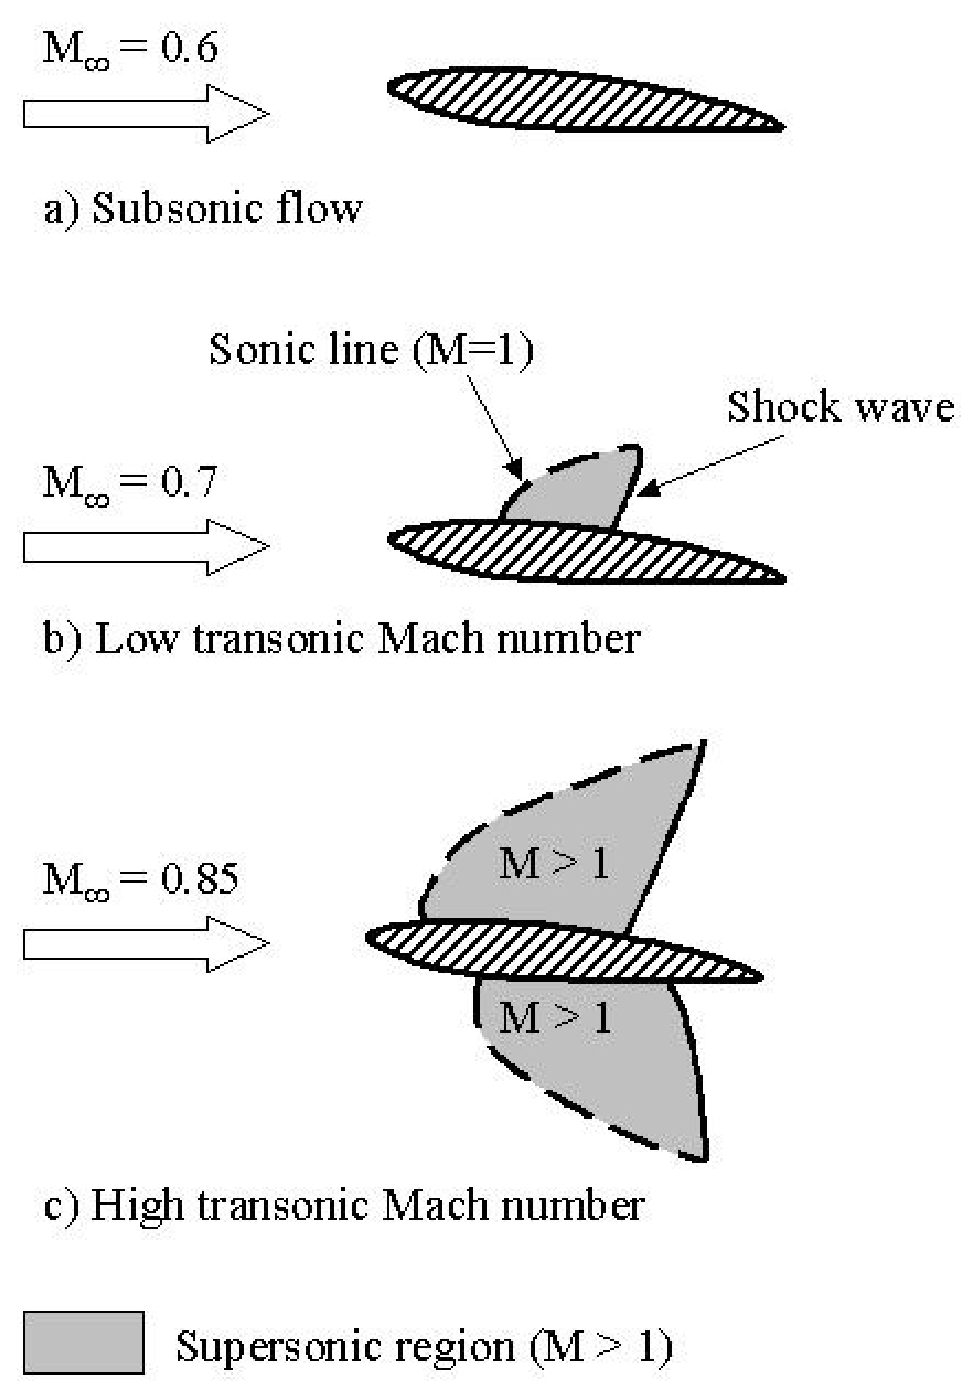
\includegraphics[height=6in]{aflow}
%%%%     \else
%%%%       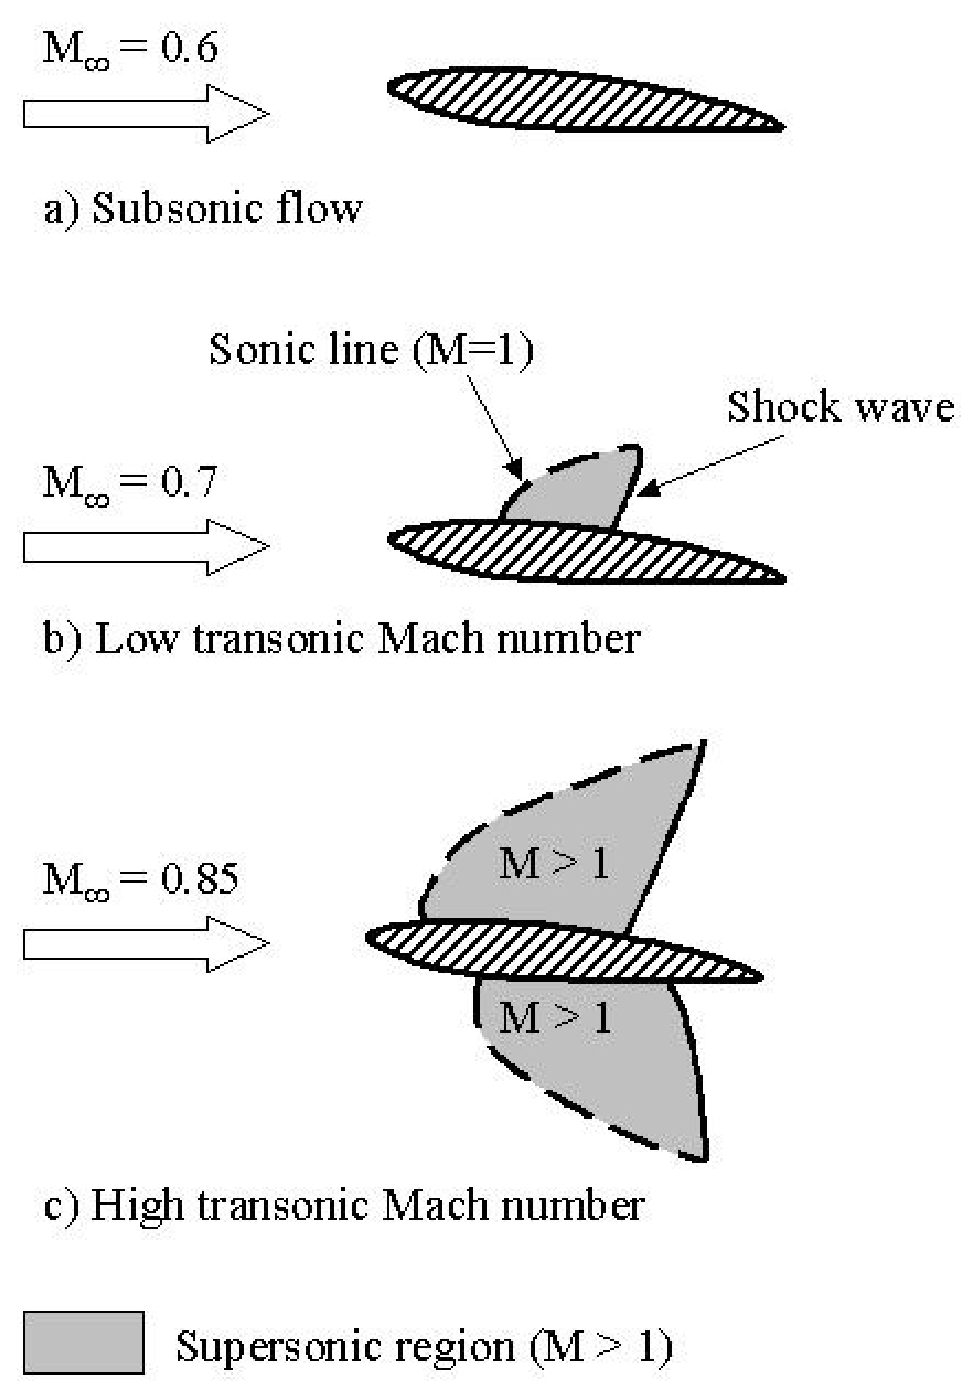
\includegraphics[bb = 92 86 545 742, height=6in]{aflow}
%%%%     \fi
%%%%     \caption{Airfoil Picture}
%%%%     \label{FigAir}
%%%%   \end{center}
%%%% \end{figure}
%%%% 
%%%% % above code has been macro-fied in Classes/MacroFile.tex file
%%%% %\InsertFig{\IncludeGraphicsH{aflow}{6in}{92 86 545 742}}{Airfoil Picture}{FigAir}
%%%% 
%%%% So as we have now labelled it we can reference it, like so (\ref{FigAir}) and it
%%%% is on Page \pageref{FigAir}. And as we can see, it is a very nice picture and we
%%%% can talk about it all we want and when we are tired we can move on to the next
%%%% chapter ...
%%%% 
%%%% I would also like to add an extra bookmark in acroread like so ...
%%%% \ifpdf
%%%%   \pdfbookmark[2]{bookmark text is here}{And this is what I want bookmarked}
%%%% \fi


\chapter{Uniform Bounds for Functionals of Nonstationary Time Series} \la{chap:2}
\ifpdf
    \graphicspath{{Chapter2/Chapter2Figs/PNG/}{Chapter2/Chapter2Figs/PDF/}{Chapter2/Chapter2Figs/}}
\else
    \graphicspath{{Chapter2/Chapter2Figs/EPS/}{Chapter2/Chapter2Figs/}}
\fi

In this chapter, we establish uniform convergence for the sample average functional, under the situation that the sample is a general class of nonstationary time series, including integrated and fractionally integrated time series. Such kind of structure has an essential difference from the Harris recurrent Markov chain considered in Chapter \ref{chap:1}. Sharp upper and lower uniform bounds are established, and the results will be useful for the investigation of uniform convergence for kernel estimates in nonlinear cointegrating regression.

\section{Introduction}
Consider a triangular array ${x_{k,n},1\leq k\leq n,n\geq
1}$ constructed from some underlying time series.
In most practical situations, $x_{k,n}$ is equal to $x_k/d_n$, where $x_k$
is a partial sum and $0 < d_n\to \infty$ in such a way that $x_n/d_n$ has a limit distribution.  The functional of interest $ S_{2n}(x)$ of $x_{k,n}$ is defined by the sample average
\bestar
S_{2n} (x)=\sum_{k=1}^{n}g[c_{n}\,(x_{k,n}+x)], \quad x\in R,
\eestar
where $c_{n}$ is a certain sequence of positive constants and $g$ is
a real function on $R$. Such functional commonly arises in nonlinear regression with integrated time series [\citet[][\citeyear{parkphillips2001}]{parkphillips1999}] and nonparametric estimation in relation to nonlinear cointegration models [\cite{phillipspark1998}, \cite{karlsentjostheim2001}]. The limit behavior of $S_{2n}(x)$ in the situation that $c_{n}\rightarrow \infty $ and $n/c_{n}\rightarrow \infty $ is particularly interesting and important for practical applications as it provides a setting that accommodates a sufficiently wide range of bandwidth choices to be relevant for nonparametric kernel estimation.

For a fixed $x$, the limit distribution of $S_{2n}(x)$ has been established by many authors. For example, \cite{borodinibragimov1995}, \cite{akonom1993} and \cite{phillipspark1998} investigated the particular situation where $x_{k}$ was a partial sum of i.i.d. random variables. \cite{jeganathan2004} studied the asymptotic form of similar functionals when $x_{k}$ was a partial sum of long memory linear processes. \cite{wangphillips2010a} improved the above papers by allowing more general conditions on $x_t$.  \cite{wangphillips2010b} considered the point-wise asymptotics of a class of zero energy functionals.  

The aim of this chapter is to investigate uniform (upper and lower) bounds  for $S_{2n}(x)$ on a compact set or on $R$. As discussed in the introduction of this thesis, these results will be useful for the investigation of uniform convergence for kernel estimates in a nonlinear cointegrating regression model. In this regard, for a near $I(1)$ regressor $x_t$, \cite{wangwang2012} established uniform consistency for  both the regression and the volatility functions under  a compact set. Without the compact set restriction,  \cite{gaolitjostheim2011} derived strong and weak consistency results for the case where $x_k$ was a null recurrent Markov chain,  but  imposed independence between $u_k$ and $x_k$. The independence condition in \cite{gaolitjostheim2011} was removed in our Chapter \ref{chap:1}, where we also investigate the uniform convergence for a class of martingales.

 The present chapter has a similar goal to \cite{gaolitjostheim2011} and Chapter \ref{chap:1}. However, instead of the null recurrent Markov chain, we work on the
  general nonstationary regressor $x_k$ that is similar to \cite{wangphillips2010a}, including a partial sum of general linear processes. As noticed in \cite{wangphillips2010a}, this kind of regressor has an essential difference from the null recurrent Markov chain, and is more natural for econometric applications. Furthermore, our uniform convergence rates are sharp and may be optimal.

 It should be mentioned that the results established in this chapter have applications not only in nonlinear cointegration model, but also in other areas such as nonlinear autoregression and  nonlinear regression with nonlinear nonstationary heteroskedasticity (NNH) errors. For the latter case, we refer to \cite{wangwang2012} and the reference therein for more details.

This chapter is organized as follows. Section \ref{sec:2:main} presents the uniform (upper and lower) bounds for a class of functionals  of nonstationary time series. Theorem \ref{thm:2:MainLower} gives the bounds for general nonstationary time series and Corollary \ref{corZero} provides the results when $x_t$ is a partial sum of linear processes. Technical proofs are postponed to Section \ref{sec:2:proof}.

\section{Main results} \la{sec:2:main}

We make use of the following assumptions in the development of main results.

\begin{assump} \la{assump:2:lipschitz}
	$\sup_x|g(x)|<\infty$, $\int_{-\infty}^{\infty}|g(x)|dx<\infty$ \textit{and }\textit{\
	$|g(x)-g(y)|\le C|x-y|$ whenever  $|x-y|$ is sufficiently small on }$R$.
\end{assump}

\begin{assump} \la{assump:2:weakConvergence}
\textit{There exists a stochastic process }%
$G$\textit{\ having a continuous local time
}$L_{G}(t,s)$\textit{\ such that }$x_{[nt],n}\Rightarrow
G(t)$\textit{, on }$D[0,1],$\textit{\ where
weak convergence is understood w.r.t the Skorohod topology on the space }$%
D[0,1]$\textit{.}
\end{assump}

\begin{assump} \la{assump:2:density}
 \textit{For all }$0\leq k<l\leq n,n\geq 1$ \textit{, there exist a sequence of constants }$d_{l,k,n}\sim C_0 [n/(l-k)]^{-d}$\textit{\ for some $0< d<1$
and a
sequence of increasing }$\sigma $\textit{-fields }${\mathcal F}_{k,n}$\textit{\ (define }$%
{\mathcal F}_{0,n}=\sigma \{\phi ,\Omega \}$\textit{, the trivial }$\sigma $\textit{%
-field) such that} $x_{k,n}$\textit{\ are adapted to }${\mathcal F}_{k,n}$\textit{\
and, conditional on }${\mathcal F}_{k,n}$\textit{,
}$(x_{l,n}-x_{k,n})/d_{l,k,n}$\textit{\ has a density
}$h_{l,k,n}$\textit{\ satisfying that }$h_{l,k,n}$\textit{\ is
uniformly bounded by a constant }$K$\textit{\ and uniformly for $j-k$ sufficiently large}
\be
 \sup_y | h_{l,k,n}(y + u) - h_{l,k,n}(y)| \le C \min\{|u|, 1\}. \la {eqn:2:77}
\ee
\end{assump}

We mention that Assumption \ref{assump:2:lipschitz} is standard in the investigation of uniform convergence,
which provides rich choices for kernel estimation applications. Assumptions \ref{assump:2:weakConvergence} and \ref{assump:2:density} are similar to those used in Theorem 2.1 of \cite{wangphillips2010a} (see Appendix \ref{chap:app3}). The additional requirement on $d_{l,k,n}$ is mild, which is used here for technical convenience.
Indeed, in  most practical situations, $x_{k,n}=\sum_{j=1}^k \eta_j/d_n$, where $d_n^2= var (\sum_{j=1}^n\eta_j)\sim C_0n^{2d}$ for some $0< d<1$, as stated in the following Examples 3.1 and 3.2. In this situation, it is natural to set $d_{l,k,n}\sim C_0 [n/(l-k)]^{-d}$.


\medskip
{\bf Example 3.1.} Let $\{ \xi_j, j \ge 1\}$ be a stationary sequence of Gaussian random variables  with $\E \xi_1 = 0$ and covariances $\gamma( j - i) = \E \xi_j \xi_i$ satisfying the following conditions for some $0 < \beta < 2$ and $\lambda > 1$,
\be
d_n^2 \equiv \sum_{1 \le i,j\le n} \gamma(j-i) \sim n^\beta \quad  and \quad  | \tilde{\gamma}_{l,k} | \le \lambda d_k d_{l-k},
\ee
as $\min \{k, l-k\} \to \infty$, where
\be
\tilde{\gamma}_{l,k} = \sum_{i = 1}^k \sum_{j = k+1}^l \gamma(j-i)
\ee
Let $x_{k,n}= \sum_{j = 1}^k \xi_j/d_n$, $1 \le k \le n$. Then $x_{k,n}$ satisfies Assumptions \ref{assump:2:weakConvergence} and \ref{assump:2:density} with $G(t) = W_{\beta/2}(t)$.   See Corollary 2.1 of \cite{wangphillips2010a}.

\medskip
{\bf Example 3.2.} Let $\{\xi_{j},j\geq 1\}$ be a linear process defined by
$
\xi _{j}=\sum_{k=0}^{\infty }\,\phi _{k}\,\epsilon _{j-k},
$
where $\{\epsilon _{j},-\infty <j<\infty \}$ is a sequence of i.i.d.
random variables with $E\epsilon _{0}=0$, $E\epsilon _{0}^{2}=1$, $\E|\ep_0|^r < \infty$ for some $r > 2$ and the
characteristic function $\varphi $ of $\epsilon _{0}$ satisfies
$\int_{-\infty
}^{\infty }(1+|t|)|\varphi (t)|dt<\infty $. The coefficients $\phi_k$, $k \ge 0$ are assumed to satisfy one of the following conditions:
\begin{itemize}
\item[\textbf{C1.}] $\phi _{k}\sim k^{-\mu }\,\rho(k),$ where $1/2<\mu <1$ and $%
\rho$ is a function slowly varying at $\infty $.
\item[\textbf{C2.}] $\sum_{k=0}^{\infty } |\phi _{k}|<\infty $ and $\phi \equiv
\sum_{k=0}^{\infty }\phi_{k}\not =0$.
\end{itemize}

Write $x_{t}=\sum_{j=1}^t \xi_{j}$ and $d_n^2 = \E x_n^2$. We have
\be \la{sec2.f2}
d_n^2 = \E x_n^2 \sim
\begin{cases}
c_{\mu} n^{3-2\mu} \rho^2(n),  & \mbox{under {\bf C1},} \\
\phi^2 n, & \mbox{under {\bf C2},}
\end{cases}
\ee
where $c_\mu = \frac{1}{(1 - \mu)(3-2\mu )} \int_{0}^{\infty} x^{-\mu} (x+1)^{-\mu} dx$. See Theorem \ref{thm:app1:asym} in Appendix \ref{chap:app1}.
In the end of Section \ref{sec:2:proofThm}, we prove that  $x_{k,n}\equiv x_k/d_n, 1\le k\le n,$ satisfies Assumptions \ref{assump:2:weakConvergence} and \ref{assump:2:density} with
\be
 G(t) &=&\begin{cases}
 W_{\mu - 3/2}(t),  & \mbox{under {\bf C1},} \\
W(t), & \mbox{under {\bf C2}.}
\end{cases} \la {im19}
\ee


\medskip
We now state our main results.







\begin{thm} \la {thmMainUpper}  Under Assumptions \ref{assump:2:lipschitz} and \ref{assump:2:density}, we have
\be \la{thmMainUpper.eqn1}
\sup_{|x|\le n^{m_0}} |S_{2n}(x)| =O[(n/c_n)\log n],\quad a.s., \la {eqn:2:ad1}
\ee
 for any $c_n\to\infty$ and $c_n/n\to 0$, and any fixed constant $0<m_0<\infty$. If there exist positive constants  $m$ (allow to be sufficiently large) and
 $k$ (allow to be sufficiently small) such that $n\sup_{|x|>n^{m}/2}|g(c_n\, x)|=O[(n/c_n)\log n]$  and $
n^{-m k} \sum_{t=1}^n |x_{t,n}|^k  = O(1)\, a.s.,
$
then
\be
\sup_{x\in R} |S_{2n}(x)| =O[(n/c_n)\log n], \quad a.s. \la {eqn:2:69}
\ee
\end{thm}


If we are only concerned with convergence in probability, the bound can be improved,  as stated in the following theorem.

\begin{thm} \la{thm:2:MainLower}  Under Assumptions \ref{assump:2:lipschitz}--\ref{assump:2:density},  we have
\be\la{eqn:2:MainLower0}
\sup_{|x|\le M_0/ \log^{\gamma_1} n} |S_{2n}(x)| =O_P(n/c_n),\quad 
\ee
where
 \be
 \gamma_1 &=&\begin{cases}
 4\,\big (\frac{d}{1-d}\big),  & \quad if \quad  0 < d \le 3/5, \\
\big ( \frac{1+d}{1-d} \big ) \big ( \frac{d}{1-d} \big ), &\quad if \quad 3/5<d <1,
\end{cases} \la {eqn:2:gamma}
\ee
for any fixed $M_0>0$, $c_n\to\infty$ and $(n/c_n) \log^{-\theta_1}n \to \infty$, where $\theta_1 = (1-d)\gamma_1/d$. If in addition  $\int_{-\infty}^{\infty} g(x)dx\not=0$,  then
\be \la{eqn:2:MainLower1}
\Big [ \inf_{|x|\le M_0/ \log^{\gamma_1} n}| S_{2n}(x)|\Big]^{-1} =\sup_{|x|\le M_0/ \log^{\gamma_1} n} |S_{2n}^{-1}(x)| =O_P(c_n/n) .
\ee
\end{thm}

\begin{rem} \la{rem:2:local} It is readily seen that $d_{l,k,n}\sim C_0 [n/(l-k)]^{-d}$ for some $0< d<1$ satisfies Assumption 2.3 (i) of \cite{wangphillips2010a}.
If in addition to Assumptions \ref{assump:2:lipschitz}--\ref{assump:2:density}, $\int_{\infty}^{\infty} g(x)dx\not=0$.  Theorem 2.1 and Remark 2.1 of \cite{wangphillips2010a} yield that
\be
\frac{c_n}{n}\sum_{t = 1}^{n} g[c_n\, (x_{t,n}+y_n)] \to_D \int_{-\infty}^{\infty} g(x)dx\, L_G(1,y), \la {eqn:2:99}
\ee
whenever $c_n\to\infty$, $n/c_n\to\infty$ and $y_n\to y$. This, together with the fact that $P(L_G(1, x)=0)>0$ for any fixed $x\not=0$ (see Theorem \ref{thm:app2:localDist} in Appendix \ref{chap:app2}) implies that both convergence rates in (\ref {eqn:2:MainLower0}) and (\ref {eqn:2:MainLower1}) are optimal and  the range  $|x|\le M_0/ \log^{\gamma_1} n$ in   (\ref {eqn:2:MainLower1}) can not be improved  to $|x|\le b$ for any constant $b>0$. In Chapter \ref{chap:3}, we use a complete different technique to establish a stronger version of Theorem \ref{thm:2:MainLower}. Corollary \ref{cor1} provides an optimal range to make result (\ref {eqn:2:MainLower1}) hold. See Remark \ref{rem:3:optimal} for details.
\end{rem}


\begin{rem} Results similar to (\ref{eqn:2:MainLower0}) and (\ref{eqn:2:MainLower1}) were established  in
Chapter \ref{chap:1} for a Harris recurrent Markov chain. As stated in \cite{wangphillips2010a}, our Assumption \ref{assump:2:density}, which includes a partial sum of general linear processes (see Examples 3.2), is more natural for econometric applications and has an essential difference from the  Markov chain.
\end{rem}


The essential idea behind the proof of Theorem \ref {thm:2:MainLower} is a fact   that $S_{2n}(x)$ can be approximated by $S_{2n}(0)$ under a reasonable rate. Explicitly we have the following theorem.

\begin{thm} \la{thm:2:thm7} Let $\gamma \ge 0$. Under Assumptions \ref{assump:2:lipschitz}--\ref{assump:2:density},  we have
\be
\sup_{|x|\le M_0\, D_n / \log^{\gamma} n } |S_n(x)-S_n(0)| =O_P\big [(n / c_n) D_n^{\lambda_2}\log^{1-\lambda_1}n\, + (n / c_n)^{1/2}\big ],\quad  \la {eqn:2:ad121a}
\ee
 for any $(c_n / n)^{\rho} \le D_n\le 1$, $0\le \rho<\min\{1/\lam_2, \, 1/d^*\}$,  $c_n\to\infty$ and $(n/c_n) \log^{-\theta}n \to \infty$, where $M_0>0$ is a fixed constant, $\theta = \max\{(\lambda_1+1)/(1-\rho\lam_2),\ \eta / (1 - \rho d^*)\}$,  and
\be \la {eqn:2:h1}
\lambda_1 = \begin{cases}
\frac{(1-d)^2\gamma/d-(2d-1)}{2-d},  & \mbox{ if    $1/2 < d < 1$  and  $\gamma \ge d(5d-1)/(2d-1)$}, \\
\frac{(1+\gamma)(1-d)-2d}{1+d},  & otherwise, \\
\end{cases}
\ee
\be \la {h2}
\lambda_2 =  \begin{cases}
\frac{1 - d}{1 + d},  &  if \quad    0 < d < 1/2, \\
\frac{(1 - d)^2}{d(2-d)},  &  if \quad   1/2 \le d < 1, \\
\end{cases} \quad \quad
d^* = \begin{cases}
\frac{2-d}{1+d},  & if \quad   0 < d < 1/2, \\
\frac{1 - d}{d}, & if \quad  1/2 \le d < 1, \\
\end{cases}
\ee
\be \la{eqn:2:eta}
\eta = \begin{cases}
\gamma + \frac{(\lambda_1+1) (1-2d)}{1-d},  & if \quad   0 < d < 1/2, \\
\gamma -1, & if \quad  d = 1/2, \\
\frac{(1-d)\gamma}{d}, & if \quad  1/2 < d < 1.
\end{cases}
\ee
In particular, take $\rho = 0$, i.e. $D_n = 1$, we have
\be
\sup_{|x|\le M_0/ \log^\gamma n} |S_n(x)-S_n(0)| =O_P[(n/c_n) \log^{1-\lambda_1} n + (n / c_n)^{1/2}],\quad  \la {ad121}
\ee
provided $c_n\to\infty$ and $(n/c_n) \log^{-\theta_0}n \to \infty$, where  $\theta_0 = \max\{\lambda_1+1,\ \eta \}$.

\end{thm}

\begin{rem}
Note that $S_n(0)=O_P[(n / c_n)^{1/2}]$ under certain conditions by \cite{wangphillips2010b}. By taking $D_n$ small, the result (\ref {eqn:2:ad121a}) can be used to investigate
 the uniform convergence for zero energy function of nonstationary time series.
 See (\ref {ad1211}) in the following  Corollary \ref {corZero}  for an example.
\end{rem}


\begin{cor} \la{corZero} Suppose Assumption \ref{assump:2:lipschitz} holds, and  $x_t$ and $d_n^2=var (x_n)$ are defined as in Example 3.2. Then,
for any $h$ satisfying $h\to 0$ and $n^{ 1- \de_0} h/d_n \to \infty$, where  $\de_0>0$ can be made as small as required, we have
\be
\sup_{|x|\le  M_0\,d_n/\log^{\gamma_0} n} \big|\sum_{t = 1}^n g\Big (\frac{x_t - x}{h} \Big )\big| =O_P (nh / d_n),\quad  \la {h11}
\ee
where $M_0$ is a fixed constant and
\be
\gamma_0 &=&\begin{cases}
\frac {4(3-2\mu)}{2\mu-1},  & \quad \mbox{under {\bf C1} and $9/10<\mu<1$ }, \\
\frac {(5-2\mu)(3-2\mu)}{(2\mu-1)^2}, & \quad \mbox{under {\bf C1} and $1/2<\mu\le 9/10$, }\\
4, &\quad  \mbox{under {\bf C2}. }
\end{cases} \la {al2}
\ee
If in addition  $\int_{-\infty}^{\infty} g(x)dx\not=0$,  then
\be \la{h12}
\Big [ \inf_{|x|\le  M_0\,d_n/\log^{\gamma_0} n}\big|\sum_{t = 1}^n g\Big (\frac{x_t - x}{h} \Big )\big|\Big]^{-1}  =O_P[d_n/(nh)] .
\ee
Furthermore, if in addition $h\to0$ ($h^2\log n\to 0$ under {\bf C2}),
 $\int|\hat g(t)|dt<\infty$ and $|\hat g(t)|\le C\min\{|t|,1\}
 $, where $\hat g(t)=\int e^{itx}g(x)dx$, then
\be
\sup_{|x|\le  B_n} \big|\sum_{t = 1}^n g\Big (\frac{x_t - x}{h} \Big )\big| =O_P\big [ (nh / d_n)\,a_n^{\Lambda}+(nh/d_n)^{1/2}\big ],\quad  \la {ad1211}
\ee
where $B_n=M_0a_nd_n/\log^{\gamma_0}n$, $(nh/d_n)^{-1/2}\le a_n^{\Lambda}\le 1$ and
\be
 \Lambda &=&\begin{cases}
\frac{(2\mu - 1)^2}{(3 - 2\mu) (1 + 2\mu)},  & \quad \mbox{under {\bf C1}}, \\
1 / 3, &\quad \mbox{under {\bf C2}}.
\end{cases}
\ee
\end{cor}

\begin{rem} \la{rmk:2:shorter} Since the conditions that $\int|\hat g(t)|dt<\infty$ and $|\hat g(t)|\le C\min\{|t|,1\}$ imply $\int g(x)dx=0$ [see, e.g., \cite{wangphillips2010b}], the result
(\ref {ad1211}) provides the uniform convergence rate for   zero energy functionals of an $I(1)$ process. Recalling  Theorem 2.1 of \cite{wangphillips2010b}, the optimal
convergence rate $(nh/d_n)^{1/2}$ is obtained by taking $a_n=(nh/d_n)^{-1/(2\Lambda)}$. For this $a_n$, under {\bf C2} (i.e., $\Lambda=1/3$, $\gamma_0=4$ and $d_n=\sqrt n$), we have
\bestar
B_n &=& M_0(\sqrt nh)^{-3/2}\sqrt n/\log^4n =M_0(nh^6\log n)^{-1/4}.
\eestar
Hence, whenever $nh^6\log n\to 0$, a reasonable range on $x$ in (\ref {ad1211}) is achievable to obtain the optimal convergence rate. However, when $\mu$ is close to $1/2$ under {\bf C1}, the current result fails to provide a reasonable range on $x$ to reach the optimal convergence rate. It keeps an open problem for this issue.
\end{rem}





\section{Proofs of main results} \la{sec:2:proof}
This section provides proofs of the main results. We start with a lemma, which will be heavily used in the proof of main results.
Throughout this section, we denote constants by $C, C_1, C_2,...$, which may be different at each appearance.

\subsection{Preliminaries}

\begin{lem} \la {lem:2:lem1} Under Assumption \ref{assump:2:density}, for any real function $l$ satisfying $\sup_x|l(x)|<\infty$ and $\int_{-\infty}^{\infty}|l(x)|dx<\infty$, there exist a constant $H_0$ (not depending  on $t_1, t_2, t_3$) and $m$  such that
\be
&& \sup_x\, E\big(|\sum_{k=t_2}^{t_3}l[c_n\, (x_{k,n}+x)]|^m\mid {\mathcal F}_{n,t_1}\big) \no\\
&\le &  H_0^m \, (m+1)!\, n^d\,c_n^{-1}  (t_3-t_1)^{1-d}\big[1+ \big\{(t_3-t_2)^{1-d} n^d\,c_n^{-1}\big\}^{m-1}  \big], \la {lm90}
\ee
for all $0\le t_1<t_2<t_3\le n$ and integer $m\ge 1$. In particular, by letting $t_1=0, t_2=1$ and $t_3=n$, we have
\be
 \sup_x\, E|\sum_{k=1}^{n}l[c_n\, (x_{k,n}+x)]|^m
&\le & H_0^m \, (m+1)!\, (n/c_n)^{m} . \la {eqn:2:lm91}
\ee

\end{lem}

\begin{proof}
First recall that, conditional on ${\mathcal F}_{n,s}$, $(x_{t,n}-x_{s,n})/d_{t,s,n}$
has a density $h_{t,s,n}$ which is uniformly bounded by a constant $K$. Simple calculations show that, for $1\le s<t\le n$,
\be \E\big\{|l[c_n(x_{t,n}+x)]|\mid {\mathcal F}_{n,s}\big\}
&=&
\int_{-\infty}^{\infty}|l[c_n d_{t, s,n}\, y + c_n (x_{s, n}+x)] |h_{t, s,n}(y)dy\no\\
&\le& \frac {K}{c_n d_{t,s,n}}
\int_{-\infty}^{\infty}|l[y+  c_n (x_{s, n}+x)]|dy \no\\
&\le & K\,l_1  /(c_n d_{t,s,n}), \la {eqn:2:109}\ee
where $l_1=\int_{-\infty}^{\infty}|l(x)|dx$.
By virtue of this estimate, it follows from  conditional arguments repeatedly  that, for any $t_2\le k_1<k_2<...<k_m\le t_3$,
\bestar
&& \E \Big(\big| l[ c_n (x_{k_1,n} +x) ]\,...\, l[ c_n (x_{k_m,n} +x)]\big|\mid {\mathcal F}_{n,t_1}\Big) \no\\
&\le& \E \Big(\big| l[ c_n (x_{k_1,n} +x) ]\,...\,l[ c_n (x_{k_{m-1},n} +x)]\big|\,   \E \big(|l[ c_n (x_{k_m,n} +x)]|\mid {\mathcal F}_{n,k_{m-1}}\big)\mid {\mathcal F}_{n,t_1}\Big) \no\\
&\le& K\,l_1 \, c_n^{-1}\,  d_{k_m,k_{m-1},n}^{-1}\, \E \Big(\big| l[ c_n (x_{k_1,n} +x) ]\,...\,l[ c_n (x_{k_{m-1},n} +x)]\big|\,   \mid {\mathcal F}_{n,t_1}\Big) \no\\
&\le& ...... \no\\
&\le& (K\,l_1 )^m\, c_n^{-m}\, { d_{k_1,t_1,n}^{-1}}\,d_{k_2,k_1,n}^{-1}\cdots\, d_{k_m,k_{m-1},n}^{-1}.
\eestar
Therefore, by recalling $d_{t,s,n}\sim C_0\,[(n/(t-s)]^{-d}$ for some $0< d<1$ and letting $H_0=\max\{1,  K\,l_0\, l_1\,C_0 \}$ where $l_0=\sup_x|l(x)|$, we have
\bestar
&& \E\Big(|\sum_{k=t_2}^{t_3}l[c_n\, (x_{k,n}+x)]|^m \mid {\mathcal F}_{n,t_1}\Big) \no\\
&\le&  \max\{1, l_0^{m-1}\} \Big [ \sum_{k_1 =t_2}^{t_3}\E\Big( |l\big[ c_n(x_{t,n} +x) \big ] | \mid {\mathcal F}_{n,t_1}\Big)\no\\
&&  + 2\, \sum_{t_2 \le k_1 < k_2 \le t_3} \E\Big( |l\big[ c_n (x_{k_1,n} +x) \big ] l\big[c_n (x_{k_2,n} +x) \big ] | \mid {\mathcal F}_{n,t_1}\Big)+ ... \no\\
&&+ m!\, \sum_{t_2 \le k_1 < ... < k_m \le t_3} \E\Big( |l\big[ c_n (x_{k_1,n} +x) \big ]...\, l\big[ c_n (x_{k_m,n} +x) \big ]| \mid {\mathcal F}_{n,t_1}\Big) \Big ]\no\\
&\le&   H_0^m\,
\Big [ n^d\,c_n^{-1} \sum_{k_1 =t_2}^{t_3} (k_1-t_1)^{-d}\no\\
&& \qquad \qquad  + 2\,n^{2d}\,c_n^{-2} \sum_{t_2 \le k_1 < k_2 \le t_3}(k_1-t_1)^{-d}(k_2-k_1)^{-d} + ... \no\\
&& \qquad \qquad + m!\,n^{md}\,c_n^{-m} \sum_{t_2 \le k_1 < ... < k_m \le t_3} (k_1-t_1)^{-d}(k_2-k_1)^{-d}...(k_m-k_{m-1})^{-d}\Big ]\no\\
&\le& H_0^m \, (m+1)!\, n^d\,c_n^{-1}  (t_3-t_1)^{1-d}\big[1+ \big\{(t_3-t_2)^{1-d} n^d\,c_n^{-1}\big\}^{m-1}  \big].
\eestar
 This proves Lemma \ref {lem:2:lem1}. 
\end{proof}

\subsection{Proofs of theorems} \la{sec:2:proofThm}

\begin{proof}[\bf Proof of Theorem \ref {thmMainUpper}] Let
 \be y_j=-[n^{m_0}]-1+j\,/ m_n',\quad  j=0, 1,2,...,\,m_n, \la {eqn:2:m1a}
\ee where $m_n'=[(n/c_n)^{1/2} c^2_n]$ and $m_n=2([n^{m_0}]+1)m_n'$. It follows that
\be
\sup_{|x|\le n^{m_0}}\big|S_{2n}(x)\big|
&\le&  \max_{0 \le j \le m_n -1} \sup_{x \in [y_j, y_{j+1}]} \sum_{t =1}^n \big |g[c_n (x_{t,n} + x)]-g[c_n (x_{t,n} + y_j)]\big| \no\\
&\quad& + \max_{0 \le j \le m_n} \big |\sum_{t =1}^n g[c_n (x_{t,n} + y_j)]\big|  \no\\
&:=& \lambda_{1n} + \lambda_{2n}. \la {eqn:2:78}
\ee
It follows from Assumption \ref{assump:2:lipschitz} that
\be
 \lambda_{1n} &\le& C\, n\, c_n\max_{0 \le j \le m_n - 1} | y_{j+1} - y_{j}| = O\big [ (n/c_n)^{1/2}\big ],\la {eqn:2:m18a}
\ee
which yields $\lambda_{1n}=O(n/c_n),$ a.s., as $n/c_n\to \infty.$

We use Lemma \ref {lem:2:lem1} to estimate $\lambda_{2n}$. To this end, let $m=\log n$ in (\ref {eqn:2:lm91}).
It follows from Markov inequality and the Stirling approximation of $(m+1)!$ that, for any $M_0\ge e^{m_0+3}H_0$ where $H_0$ is given as in Lemma \ref {lem:2:lem1},
\begin{align}\la{p8}
& P \Big ( \max_{1 \le j \le m_n} \Big|\sum_{t = 1}^n g\big[ c_n(x_{t,n} +y_j) \big ]\Big| \ge M_0\, (n/c_n)\, \log n,\, i.o. \Big ) \no\\
&\le \lim_{s \to \infty} \sum_{n = s}^\infty \sum_{j = 1}^{m_n} P \Big ( \Big | \sum_{t = 1}^n g\big[ c_n(x_{t,n} +y_j) \big ] \Big |^m \ge \big [ M_0\, (n / c_n)\, \log n \big ]^{m} \Big ) \no\\
& \le  \lim_{s \to \infty} \sum_{n = s}^\infty \frac{ m_n }{[ M_0\, (n / c_n)\, \log n \big ]^m} \max_{1 \le j \le m_n} \E \Big | \sum_{t = 1}^n g\big[ c_n(x_t +y_j) \big ]\Big |^m \no\\
& \le \lim_{s \to \infty} \sum_{n = s}^\infty \frac{ m_n \, H_0^m (m+1)!}{[ M_0\,  \log n \big ]^m} \no\\
& \le C\,\lim_{s \to \infty} \sum_{n = s}^\infty \frac{ n^{m_0+1}\, H_0 ^m}{ \big [ M_0\,  \log n \big ]^m}   \sqrt{2\pi\,(m+1)}\, \Big ( \frac{m+1}{e } \Big )^{m+1} \no\\
& \le C\,\lim_{s \to \infty} \sum_{n = s}^\infty   e^{- (m_0+3) \log n}\, n^{m_0+1}\, \log n\,  \no\\
& \le C_1 \lim_{s \to \infty} \sum_{n = s}^\infty n^{-2}  = 0.
\end{align}
This proves $\lambda_{2n}=O[(n/c_n)\log n],$ a.s. Taking the estimates of $\lambda_{1n}$ and $\lambda_{2n}$ into (\ref {eqn:2:78}), we obtain the required (\ref {eqn:2:ad1}).

To prove (\ref {eqn:2:69}), we first write
\begin{align}
\sum_{k=1}^{n}g[c_{n}\,(x_{k,n}+x)] &= \sum_{k=1}^{n}g[c_{n}\,(x_{k,n}+x)] I(|x_{k,n}| \le n^{m}/2)  \no\\
&\qquad + \sum_{k=1}^{n}g[c_{n}\,(x_{k,n}+x)] I(|x_{k,n}| > n^{m}/2) \no\\
&:= \lambda_{1n}(x) + \lambda_{2n}(x) \la {eqn:2:71}
\end{align}
It follows from (\ref {eqn:2:ad1}) and $n \sup_{|x| > n^{m}}|g(c_n \, x)| = O[(n/c_n) \log n]$ that
\begin{align}
\sup_{x\in R} |\lambda_{1n}(x) |&\le \sup_{|x| \le n^{m}} |\lambda_{1n}(x)| + \sup_{|x| > n^{m}} | \lambda_{1n}(x) | \no\\
&\le O[(n/c_n)\log n] + n \, \sup_{|x| > n^{m}/2} | g(c_n \, x)| \quad a.s.  \no\\
&\le O[(n/c_n)\log n] \quad a.s., \la {eqn:2:72}
\end{align}
As for $\lambda_{2n}(x)$, we have
\begin{align}
\sup_{x\in R} |\lambda_{2n}(x)| &\le C \sum_{t = 1}^n  I(| x_{t,n}| > n^{m}/2)  \le C n^{-m k/2} \sum_{t = 1}^n  |x_{t,n}|^{k} \no\\
& = O(1) \quad a.s., \la {eqn:2:73}
\end{align}
Combining (\ref {eqn:2:71})--(\ref {eqn:2:73}), we prove (\ref {eqn:2:69}).
The proof of Theorem \ref {thmMainUpper} is now complete.
\end{proof}

\begin{proof}[Proof of Theorem \ref {thm:2:MainLower}] By taking $\lam_1=1$ in (\ref {eqn:2:h1}), we obtain $\gamma=\gamma_1$, where $\gamma_1$ is defined by (\ref {eqn:2:gamma}). Now Theorem \ref {thm:2:MainLower} follows immediately from (\ref{ad1211}) of Theorem \ref {thm:2:thm7} with $\lam_1=1$ and Remark \ref{rem:2:local}. We omit the details. 
\end{proof}

 \begin{proof}[Proof of Theorem \ref {thm:2:thm7}]
Let $\eta_n=(n/c_n)D_n^{\lambda_2}\log^{-\lambda_1}n,$ $b_n = [nD_n^w\log^{-\nu}n]$, where $\nu = (\lambda_1+1)/(1-d)$, $w = \lambda_2 / (1 - d)$ and let $T_n$ be the largest integer $s$ such that $s b_n \le n$. Also write  $y_j = -[M_0D_n/\log^{\gamma}n] - 1 +  j/  m_n',  j = 0,1,2,...,m_n,$ where $m'_n = [(n/c_n)^{1/2} c_n^2]$ and $m_n= 2([M_0D_n/\log^{\gamma}n]+1)m_n'$. It is readily seen that
\be
n/b_n \sim \log^{\nu} n D_n^{-w}, \quad n-1\le T_nb_n\le n, \quad m_n\le Cn^2, \la {eqn:2:110}
\ee
due to $c_n\to\infty$ and $c_n/n\to 0$. Furthermore, by recalling the definitions of $\lambda_1, \lambda_2$, $d^*$ and $\eta$ [see (\ref {eqn:2:h1})--(\ref {eqn:2:eta})], tedious but elementary calculations show that, whenever $\gamma\ge 0$,
\begin{align}
d\nu-\eta \le 1-2\lambda_1, \quad (d-1)\nu+\lambda_1\le -1, \quad 2d\nu-\gamma\le 1-\lambda_1, \la {eqn:2:112}  \\
-wd + d^* = 2\lambda_2,  \quad 1 - 2dw= \lambda_2. \la{112.1}
\end{align}

We now return to the proof of Theorem \ref {thm:2:thm7}. Using the similar arguments as in the proof of (\ref {eqn:2:78}),  we have
\be
&& \sup_{|x|\le D_n / \log^{\gamma}n} | S_n(x)-S_n(0)| \no\\
&\le & \max_{1\le j\le m_n} | S_n(y_j)-S_n(0)|+O_{a.s.}[( n/c_n)^{1/2}] \no\\
&\le& \max_{1\le j\le m_n}| \sum_{s=2}^{T_n-1} \Delta_{ns}(y_j)|+\max_{1\le j\le m_n}\Delta_n(y_j)+ O_{a.s.}[( n/c_n)^{1/2}],  \la {eqn:2:95}
\ee
where, for  $s = 1,..., T_n$ ,
\bestar
\Delta_{ns}(x) &=& \sum_{t = sb_n + 1}^{(s+1)b_n} \big ( g[c_n( x_{t,n}+x)]  - g(c_n\, x_{t,n}) \big ) ,\no\\
\Delta_n(x) &\le & \Big(\sum_{t =  1}^{2b_n} +\sum_{t =  T_nb_n}^{n}\Big)\,\big | g[c_n( x_{t,n}+x)]  - g(c_n\, x_{t,n}) \big |.
\eestar
Recall $\eta_n=(n/c_n)D_n^{\lambda_2}\log^{-\lambda_1}n$. Using Theorem \ref{thmMainUpper}, it is readily seen that
\bestar
\max_{1\le j\le m_n}\Delta_n(y_j)  &\le& C\big[(b_n + |n-T_nb_n|)/c_n\big]\log n \no\\
&\le& C\, (n/c_n)\log^{1 - \nu}n\,D_n^w
\le C\, \eta_n\, \log n,\quad a.s.
\eestar
This, together with (\ref {eqn:2:95}), implies that (\ref {eqn:2:ad121a}) will follow if we prove
\be
\max_{1\le j\le m_n}\Big(| \sum_{\substack{s = 2 \\ s \in even}}^{T_n} \Delta_{ns}(y_j)|+| \sum_{\substack{s = 2 \\ s \in odd}}^{T_n} \Delta_{ns}(y_j)|\Big)  &=& O_P (\eta_n \, \log n).  \la {eqn:2:21}
\ee
We only prove (\ref {eqn:2:21}) for $s\in even$. The other is similar and hence the details are omitted.
To this end, let $\F_{n, v}^*= \F_{n, (2v+1)b_n}, v\ge 0$, and $M_1 > 0$ to be chosen later,
\bestar
\Delta_{ns}'(x) &=& \Delta_{n,2s}(x)I(|\Delta_{n, 2s}(x)|\le M_1\, \eta_n ), \no\\
 \Delta_{n s}^*(x) &=& \Delta_{n, s}'(x)- \E \big(\Delta_{n, s}'(x)\mid \F_{n, s-1}^*\big).
\eestar
Under these notations, to prove (\ref {eqn:2:21}) for $s\in even$, it suffices to show
\be \lam_{1n} &:=&\max_{1\le j\le m_n}| \sum_{s=1}^{T_n/2} \Delta_{ns}^*(y_j)|
=O_P (\eta_n \, \log n), \la {eqn:2:22} \\
\lam_{2n} &:=& \max_{1\le j\le m_n}| \sum_{s=1}^{T_n/2} \E \big(\Delta_{n, 2s}(y_j)\mid \F_{n, s-1}^*\big)|
=O_P (\eta_n \, \log n), \la {eqn:2:23}\\
\lam_{3n} &:=& \max_{1\le j\le m_n}| \sum_{s=1}^{T_n/2} \Big(\Delta_{n, 2s}(y_j)I(|\Delta_{n, 2s}(y_j)|> M_1\, \eta_n )\no\\
&& \qquad\qquad +
\E \Big[\Delta_{n, 2s}(y_j)I(|\Delta_{n, 2s}(y_j)|> M_1\, \eta_n)\mid \F_{n, s-1}^*\Big] \Big) \no\\
&=& O_P (\eta_n \, \log n). \la {eqn:2:24}
 \ee

 We start with (\ref {eqn:2:23}).  Note that, for any $2sb_n<t\le (2s+1)b_n$ and $|x|\le M_0D_n / \log^{\gamma}n$ (letting $s_n=(2s-1)b_n$),
 \begin{align} \la{eqn:2:24.5}
& \Big| E\big [ g[c_n (x_{t,n} + x)] - g( c_n\, x_{t,n}) \Big | \F^*_{n, s-1} \big ]\Big|= \Big| E\big [ g[c_n (x_{t,n} + x)] - g( c_n\, x_{t,n}) \Big | \F_{n, s_n} \big ]\Big|\no\\
&\quad = \Big| \int_{-\infty}^{\infty} \Big (g[c_n (x_{s_n,n} + d_{t, s_n, n} y + x)] - g[ c_n\, (x_{s_n,n} + d_{t,s_n,n} y) ] \Big ) \, h_{t, s_n,n}(y) dy \Big|\no\\
&\quad \le d_{t,s_n,n} ^{-1}\,
 \int_{-\infty}^{\infty}  g[c_n(y+x_{s_n,n})]\big | h_{t, s_n,n}[(y - x)/ d_{t,s_n,n}] -  h_{t, s_n,n}(y/ d_{t,s_n,n}) \big |\,dy \no\\
 &\quad \le C\,  c_n^{-1}d_{t,s_n,n} ^{-1}\min\{|x|d_{t,s_n,n} ^{-1}, 1\} \le C\,|x|\, c_n^{-1} (n/b_n)^{2d}\, \no\\
 &\quad \le C\,  c_n^{-1}\, D_n^{1-2dw}\log^{2d\nu - \gamma}n ,
\end{align}
due to Assumption \ref{assump:2:density} and $d_{t,s,n}\sim C_0[n/(t-s))]^{-d}$. It is readily seen that
\be \la{eqn:2:25}
\lam_{2n} &\le& \sum_{s=1}^{T_n/2}  \max_{1\le j\le m_n} |\E \big(\Delta_{n, 2s}(y_j)\mid \F_{n, s-1}^*\big)| \no\\
&\le& C\, (n/c_n)\, D_n^{1 - 2dw}\log^{2d\nu - \gamma}n = O_P(\eta_n \, \log n),
\ee
due to (\ref {eqn:2:112}) and (\ref{112.1}), which yields (\ref {eqn:2:23}).

Next for (\ref {eqn:2:24}). Note that, due to (\ref {eqn:2:110}) and $(n/c_n)\log^{-\theta}n\to \infty$, where $\theta\le (\lam_1+1)/(1-\rho\lam_2)$. We have
\bestar
(n/c_n) (n/ b_n)^{d-1} \sim (n/c_n) D_n^{\lam_2}\log^{(d-1)\nu}n \ge [(n/c_n)\log^{-\theta}n]^{1-\lam_2\rho}\to \infty.
\eestar
Now, it follows from  Lemma \ref {lem:2:lem1} with $t_1=0, t_2=2sb_n+1$ and $t_3=(2s+1)b_n$ that,  for any integer $m\ge 1$,
\bestar
\sup_x \E |\Delta_{n, 2s}(x)|^m &\le& H_0^m (m+1)!\, (n/c_n)\, \big\{1+ \big [(n/c_n) (n/ b_n)^{d-1} \big ]^{m-1}\big\}\no\\
&\le& 2H_0^m (m+1)! (n/c_n)^m (n/b_n)^{(d - 1)(m-1)}.
\eestar
 By virtue of this fact, we have
\bestar
E\lam_{3n} &\le& 2\,\sum_{j=1}^{m_n}\,
\sum_{s=1}^{T_n/2}\E \Delta_{n, 2s}(y_j)I(|\Delta_{n, 2s}(y_j)|> M_1\, \eta_n) \no\\
&\le& 2\, m_n T_n \,\, H_0^m (m+1)!  (n/c_n)\Big [ \frac{(n/c_n)(n/b_n)^{d-1}}{M_1\,\eta_n} \Big ]^{m-1} \no\\
&\le& C\, n^4 (H_0/M_1)^m\, (m+1)!   \log^{-(m-1)} n,
\eestar
due to (\ref {eqn:2:110}), $(d-1)\nu+\lambda_1\le -1$ by (\ref {eqn:2:112}) and $(1 - d)w =\lambda_2$.
Taking $m = \log n$ and letting $M_1 \ge 5H_0$,
it follows from the Stirling approximation of $(m+1)!$ that
\be \la{26}
E\lam_{3n} &\le& C n^4 \log^5 n \exp \{-(M_1/H_0) \, \log n\} \le Cn^{-1}\log^5 n \to 0,
\ee
which implies that $\lam_{3n}=o_P(1)$. Hence (\ref {eqn:2:24}) follows.

We finally consider (\ref {eqn:2:22}). First note that, similar to the proof of (\ref {eqn:2:24.5}),
\bestar
I_{k,j}&:=&\Big|\E \Big(  \{g[c_n(x_{j,n} + x)] - g[c_n x_{j,n}] \}\mid {\mathcal F}_{n, k}\Big)\Big| \no\\
&\le& d_{j,k, n}^{-1}\,
 \int_{-\infty}^{\infty} g[c_n(x_{k,n} + y)]
 \big | h_{j, k, n}[(y - x)/ d_{j,k, n}] -  h_{j,k,n}( y/ d_{j,k,n}) \big |\,dy \no\\
 & \le& C\, c_n^{-1}\,  d_{j,k, n}^{-1} \min\{|x| d_{j,k, n}^{-1}, 1\}\no\\
 &\le & C\, c_n^{-1}\, [n/(j-k)]^d \min\{|x|[n/(j-k)]^{d},1\},
\eestar
for any $k<j$. This, together with  (\ref {eqn:2:109}), implies  that, for any $|x| \le M_0D_n / \log^{\gamma}n$,
\begin{align}
&\quad E[\Delta_{ns}^{*2}(x) | \F^*_{n, s-1}] \le 2 E[ \Delta_{n, 2s}^2(x) | \F_{n, (2s-1) b_n} ] \no\\
&\le \sum_{k = 2sb_n +1}^{(2s+1)b_n} E \Big (  \{ \, g[c_n(x_{k,n} + x)] - g[c_n x_{k,n}]\, \}^2 \,| \,\F_{n, (2s-1)b_n} \Big ) \no\\
&\quad + 2 \sum_{2sb_n + 1 \le k < j \le (2s+1)b_n} \big|E \Big ( \{g[c_n(x_{k,n} + x)] - g[c_n x_{k,n}] \} \, \no\\
&\hskip 5cm \{g[c_n(x_{j,n} + x)] - g[c_n x_{j,n}] \}\,\Big | \F_{n,(2s-1)b_n} \Big ) \big| \no\\
&\le C\, (n/c_n) (n /b_n)^{d-1}  + 2 \sum_{2sb_n + 1 \le k < j \le (2s+1)b_n}
E \Big ( |g[c_n(x_{k,n} + x)] - g[c_n x_{k,n}] |\,  |I_{k,j}|\, \Big  | \,\F_{n, (2s-1)b_n} \Big )   \no\\
&\le C\, (n/c_n) (n /b_n)^{d-1} + C\,n^{2d}\, c_n^{-2}\,b_n^{-d}  \sum_{ 2sb_n + 1\le k<j\le (2s+1)b_n}\,(j-k)^{-d}\min\{n^d\log^{-\gamma}_nD_n (j-k)^{-d}, 1\} \no\\
&\le C\, (n/c_n) (n /b_n)^{d-1} + C\,n^{2d}\, c_n^{-2}\,b_n^{1-d}\sum_{k=1}^{b_n} k^{-d} \min\{(n/k)^dD_n\log^{-\gamma}n, 1\} \no\\
&\le C\, (n/c_n) (n /b_n)^{d-1} \big[1+   \, (n/c_n) D_n^{d^*} \log^{-\eta}n\big],
\end{align}
where we have used the fact: for $0<d<1$, letting $\zeta_n =D_n^{1/d} \log^{-\gamma/d} n$,
\bestar
&& \sum_{k=1}^{b_n} k^{-d} \min\{(n/k)^dD_n\log^{-\gamma}n, 1\} \no\\
&\le& \sum_{k=1}^{n \zeta_n} k^{-d}+ n^dD_n\log^{-\gamma}n\sum_{k=n\zeta_n+1}^{b_n} k^{-2d}\no\\
&\le& C\, n^{1-d}\,D_n^{d^*} \log^{-\eta}n.
\eestar
 It follows from this estimate that
\bestar
&& \max_{0\le j\le m_n}\, \sum_{s=1}^{T_n/2}\,\E [\Delta_{ns}^{*2}(y_j)\mid {\mathcal F}_{n, s-1}^*] \no\\
&\le&  C\, (n/c_n) (n /b_n)^{d}\big[1+   \, (n/c_n) D_n^{d^*} \log^{-\eta}n\big]\no\\
&\le&C(n/c_n)^2\,D_n^{-wd + d^*}  \log^{-\eta}n \le
C\, \eta_n^2 \log n,
\eestar
due to (\ref {eqn:2:112}), $D_n \ge (c_n/n)^\rho$ and $(n/c_n)\log^{-\eta / (1 - \rho d^*)}n \to \infty$.
This, together with the facts that  $|\Delta_{ns}^{*}(y_j)|\le \eta_n$ and for each $j$,
$\{\Delta_{ns}^{*}(y_j), {\mathcal F}_{n, s}^*\}$ forms a martingale difference, it follows from
the well-known martingale exponential inequality
(see, e.g., de la Pana (1999)) that, there exists a $M_0\ge 3$ such that, as $n \to \infty$,
\be
&& P[\lam_{1n} \ge  M_0 \eta_n\, \log n] \no\\
&\le&
 P\Big[\lam_{1n} \ge  M_0 \eta_n \, \log n,\ \
 \max_{0\le j\le m_n}\, \sum_{s=1}^{T_n/2}\,\E [\Delta_{ns}^{*2}(y_j)\mid {\mathcal F}_{n, s-1}^*]\le C\, \eta_n^2\, \log n  \Big] + o(1)\no\\
 &\le& \sum_{j=0}^{m_n} P\Big[\sum_{s=1}^{T_n/2} \Delta_{ns}^*(y_j)\ge M_0 \eta_n\, \log n, \ \
 \sum_{s=1}^{T_n/2}\,\E [\Delta_{ns}^{*2}(y_j)\mid {\mathcal F}_{n, s-1}^*]\le C\,\eta_n^2 \, \log n \Big] + o(1) \no\\
 &\le&m_n\, \exp\Big\{-\frac {M_0^2 \,\log^2 n} {2C\log n+2M_0\log n} \Big \} + o(1) \no\\
 &\le&m_n\, \exp \{-M_0\log n \} + o(1) \to 0, \la {eqn:2:p10}
\ee
where the last inequality follows from (\ref {eqn:2:110}).
 This yields $\lam_{1n}=O_P\big( \eta_n \, \log n \big )$.
Combining (\ref {eqn:2:25})--(\ref {eqn:2:p10}), we establish (\ref {eqn:2:21}).
\end{proof}

\begin{proof}[Proof of Corollary \ref {corZero}] Let $c_n = d_n / h$  and
\be
 d &=&\begin{cases}
3 / 2 - \mu,  & \quad \mbox{under {\bf C1}}, \\
1 / 2, &\quad \mbox{under {\bf C2}}. \la{prf.corZero.eqn0}
\end{cases}
\ee
It is readily seen that
\bestar
(n / c_n) \log^{-\theta}n = (nh / d_n) \log^{-\theta} n \le n^{1- \de_0} h / d_n \to \infty.
\eestar
for any $\theta\in R$. On the other hand, $x_{n,k}=x_k/d_n$ satisfies Assumption \ref{assump:2:weakConvergence} and \ref{assump:2:density}, as stated in Example 3.2.
Now, by using Theorem \ref{thm:2:MainLower} with $c_n = d_n / h$ and  the $d$ above, (\ref{h11}) and (\ref{h12}) follow from (\ref{eqn:2:MainLower0}) and (\ref{eqn:2:MainLower1}) respectively, since, with the $d$ defined by (\ref {prf.corZero.eqn0}),  the $\gamma_1$ defined by (\ref {eqn:2:gamma}) can be written as:
 under {\bf C1},
\begin{align}
 \gamma_1
&= \begin{cases}
\frac {4(3-2\mu)}{2\mu-1},  & \quad if \quad 9/10<\mu<1 , \\
\frac {(5-2\mu)(3-2\mu)}{(2\mu-1)^2}, & \quad if \quad 1/2<\mu\le 9/10, \\
\end{cases}\no
\end{align}
and under {\bf C2}, $\gamma_1 = 4$.
Using similar arguments, (\ref{ad1211}) follows from (\ref{eqn:2:ad121a}) of Theorem \ref{thm:2:thm7}  with $D_n = a_n$, $\lam_1=1$, $\lambda_2 = \Lambda$ and the following fact [see Theorem 2.1 of \cite{wangphillips2010b}]:
\bestar
S_n(0) = \sum_{t = 1}^n g\Big ( \frac{x_t}{h} \Big ) = O_P\big [( nh / d_n)^{1/2}\big].
\eestar
\end{proof}

\begin{proof}[Verification of Example 3.2]
This is similar to  the proof of Corollary 2.2 in \cite{wangphillips2010a}. The only additional work is to show (\ref{eqn:2:77}) hold as well. In fact, by writing
\be
x_l &=&\sum_{j=1}^{l}\,\sum_{i=-\infty}^{j}\ep_i\phi_{j-i} \no\\
  &=& \,x_{k}+\sum_{j=k+1}^{t}\,\sum_{i=-\infty}^{k}\ep_i\phi_{j-i} + \sum_{j=k+1}^{l}\,\sum_{i=k+1}^{j}\ep_i\phi_{j-i} \no\\
  &:=& x_{k, l}^*+x_{k,l}', \la {m-01}
  \ee
the similar arguments as in the proof of Corollary 2.2
in \cite{wangphillips2010a} yields that
 $x'_{k,l} / d_{l - k}$, where $d_n$ is defined as in (\ref {sec2.f2}),
  has a density $h_{l,k}$ and $\int_{-\infty}^{\infty} (1 + |t|)|\varphi_{l,k}(t)| dt<\infty$ uniformly for $0 \le k < l \le n$, where $\varphi_{l,k}(t) = Ee^{itx'_{l,k}/d_{l-k}}$, due to $\int (1+|t|)|Ee^{it\ep_0}|dt<\infty$.
  Hence, conditional on $\F_{k,n} = \si(\ep_j, -\infty < j \le k)$,
\be
(x_{l,n} - x_{k,n})  / d_{l,k,n} \mbox{ has a density } h_{l,k}(x - x^*_{k, l} / d_{l - k})
\ee
where $x_{t,n} = x_t / d_n$ and $d_{l,k,n} =  d_{l-k}/ d_n$. Furthermore, for any $u\in R$, we have
\bestar
&&\sup_x \big|h_{l,k}(x - x^*_{k, l} / d_{l - k}+u)-h_{l,k}(x - x^*_{k, l} / d_{l - k})\big| \no\\
&\le&
\sup_x | h_{l,k}(x +u) - h_{l,k}(x)| \no\\
&\le & C \Big | \int_{-\infty}^{\infty} \big ( e^{-it(x+u)} - e^{-itx} \big ) \varphi_{l, k}(t) dt \Big | \no\\
&\le& C\,\min\{|u |, 1\}\,  \int_{-\infty}^{\infty}  (1+|t|)\,  |\varphi_{l, k}(t)| dt  \le C_1\,  \min\{|u |, 1\},
\eestar
which yields the claim.
\end{proof}


%\begin{proof}[Proof of Theorem \ref {thm:2:MainLower}] It follows immediately from Theorem \ref {thm:2:thm7} and Remark 3.2. We omit the detalis.\end{proof}
%
%\begin{proof}[Proof of Theorem \ref {thm:2:thm7}]
%Let $\eta_n=(n/c_n)\log^{-\lambda}n,$ $b_n = [n \log^{-\nu} n]$, where $\nu=(\lambda+1)/(1-d)$, and let $T_n$ be the largest integer $s$ such that $s b_n \le n$. Also write  $y_j = -M_0/\log^\gamma n +  j/  m_n',  j = 0,1,2,...,m_n,$ where $m'_n = [(n/c_n)^{1/2} c_n^2]$ and $m_n= [M_0m_n'/\log^\gamma n]+1$. It is readily seen that
%\be
%n/b_n \sim  \log^\nu n, \quad T_nb_n\le n, \quad m_n\le Cn^2, \la {eqn:2:110}
%\ee
%due to $c_n\to\infty$ and $c_n/n\to 0$. Furthermore, by recalling the definitions of $\lambda$ and $\eta$, tedious but elementary calculations show that, whenever $\gamma\ge 0$,
%\be
%d\nu-\eta \le 1-2\lambda, \quad (d-1)\nu+\lambda\le -1, \quad 2d\nu-\gamma\le 1-\lambda. \la {eqn:2:112}
%\ee
%
%
%We now return to the proof of Theorem \ref {thm:2:thm7}. Using the similar arguments as in the proof of (\ref {eqn:2:78}),  we have
%\be
%&& \sup_{|x|\le M_0/\log^\gamma n} | S_{2n}(x)-S_{2n}(0)| \no\\
%&\le & \sup_{|x|\le M_0/\log^\gamma n} | S_{2n}(y_j)-S_{2n}(0)|+O_{a.s.}[( n/c_n)^{1/2}] \no\\
%&\le& \max_{1\le j\le m_n}| \sum_{s=2}^{T_n-1} \Delta_{ns}(y_j)|+\max_{1\le j\le m_n}\Delta_n(y_j)+ O_{a.s.}[( n/c_n)^{1/2}],  \la {eqn:2:95}
%\ee
%where, for  $s = 1,..., T_n$ ,
%\bestar
%\Delta_{ns}(x) &=& \sum_{t = sb_n + 1}^{(s+1)b_n} \big ( g[c_n( x_{t,n}+x)]  - g(c_n\, x_{t,n}) \big ) ,\no\\
%\Delta_n(x) &\le & \Big(\sum_{t =  1}^{2b_n} +\sum_{t =  T_nb_n}^{n}\Big)\,\big | g[c_n( x_{t,n}+x)]  - g(c_n\, x_{t,n}) \big |.
%\eestar
%Recall $\eta_n=(n/c_n)\log^{-\lambda}n$. Using Theorem \ref{thmMainUpper}, it is readily seen that
%\bestar
%\max_{1\le j\le m_n}\Delta_n(y_j)  &\le& C\big[(b_n + |n-T_nb_n|)/c_n\big]\log n \no\\
%&\le& C\, (n/c_n)\, \log^{1-\nu} n
%\le C\, \eta_n\, \log n,\quad a.s.
%\eestar
%This, together with (\ref {eqn:2:95}), implies that (\ref {eqn:2:MainLower1}) will follow if we prove
%\be
%\max_{1\le j\le m_n}\Big(| \sum_{\substack{s = 2 \\ s \in even}}^{T_n} \Delta_{ns}(y_j)|+| \sum_{\substack{s = 2 \\ s \in odd}}^{T_n} \Delta_{ns}(y_j)|\Big)  &=& O_P (\eta_n \, \log n).  \la {eqn:2:21}
%\ee
%We only prove (\ref {eqn:2:21}) for $s\in even$. The other is similar and hence the details are omitted.
%To this end, let $\F_{n, v}^*= \F_{n, (2v+1)b_n}, v\ge 0$, and $M_1 > 0$ is chosen later,
%\bestar
%\Delta_{ns}'(x) &=& \Delta_{n,2s}(x)I(|\Delta_{n, 2s}(x)|\le M_1\, \eta_n ), \no\\
% \Delta_{n s}^*(x) &=& \Delta_{n, s}'(x)- \E \big(\Delta_{n, s}'(x)\mid \F_{n, s-1}^*\big).
%\eestar
%Under these notation, to prove (\ref {eqn:2:21}) for $s\in even$, it suffices to show
%\be \lam_{1n} &:=&\max_{1\le j\le m_n}| \sum_{s=1}^{T_n/2} \Delta_{ns}^*(y_j)|
%=O_P (\eta_n \, \log n), \la {eqn:2:22} \\
%\lam_{2n} &:=& \max_{1\le j\le m_n}| \sum_{s=1}^{T_n/2} \E \big(\Delta_{n, 2s}(y_j)\mid \F_{n, s-1}^*\big)|
%=O_P (\eta_n \, \log n), \la {eqn:2:23}\\
%\lam_{3n} &:=& \max_{1\le j\le m_n}| \sum_{s=1}^{T_n/2} \Big(\Delta_{n, 2s}(y_j)I(|\Delta_{n, 2s}(y_j)|> M_1\, \eta_n )\no\\
%&& \qquad\qquad +
%\E \Big[\Delta_{n, 2s}(y_j)I(|\Delta_{n, 2s}(y_j)|> M_1\, \eta_n)\mid \F_{n, s-1}^*\Big] \Big) \no\\
%&=& O_P (\eta_n \, \log n). \la {eqn:2:24}
% \ee
%
% We start with (\ref {eqn:2:23}).  Note that, for any $2sb_n<t\le (2s+1)b_n$ and $|x|\le M_0/\log^\gamma n$ (letting $s_n=(2s-1)b_n$),
% \begin{align} \la{eqn:2:24.5}
%& \Big| E\big [ g[c_n (x_{t,n} + x)] - g( c_n\, x_{t,n}) \Big | \F^*_{n, s-1} \big ]\Big|= \Big| E\big [ g[c_n (x_{t,n} + x)] - g( c_n\, x_{t,n}) \Big | \F_{n, s_n} \big ]\Big|\no\\
%&\quad = \Big| \int_{-\infty}^{\infty} \Big (g[c_n (x_{s_n,n} + d_{t, s_n, n} y + x)] - g[ c_n\, (x_{s_n,n} + d_{t,s_n,n} y) ] \Big ) \, h_{t, s_n,n}(y) dy \Big|\no\\
%&\quad \le d_{t,s_n,n} ^{-1}\,
% \int_{-\infty}^{\infty}  g[c_n(y+x_{s_n,n})]\big | h_{t, s_n,n}[(y - x)/ d_{t,s_n,n}] -  h_{t, s_n,n}(y/ d_{t,s_n,n}) \big |\,dy \no\\
% &\quad \le C\,  c_n^{-1}d_{t,s_n,n} ^{-1}\min\{|x|d_{t,s_n,n} ^{-1}, 1\} \le C\,|x|\, c_n^{-1} (n/b_n)^{2d}\, \no\\
% &\quad \le C\,  c_n^{-1}  \log^{2 d\nu-\gamma}n,
%\end{align}
%due to Assumption \ref{assump:2:density} and $d_{t,s,n}\sim C_0[n/(t-s))]^{-d}$. It is readily seen that
%\be \la{eqn:2:25}
%\lam_{2n} &\le& \sum_{s=1}^{T_n/2}  \max_{1\le j\le m_n} |\E \big(\Delta_{n, 2s}(y_j)\mid \F_{n, s-1}^*\big)| \no\\
%&\le& C\, (n/c_n)\, \log^{2d\nu-\gamma}n = O_P(\eta_n \, \log n),
%\ee
%due to (\ref {eqn:2:112}),
%which yields (\ref {eqn:2:23}).
%
%Next for (\ref {eqn:2:24}). Using Lemma \ref {lem:2:lem1} with $t_1=0, t_2=2sb_n+1$ and $t_3=(2s+1)b_n$,  for any integer $m\ge 1$,
%\bestar
%\sup_x \E |\Delta_{n, 2s}(x)|^m &\le& H_0^m (m+1)!\, (n/c_n)\, \big\{1+ \big [(n/c_n) (n/ b_n)^{d-1} \big ]^{m-1}\big\}\no\\
%&\le& 2H_0^m (m+1)! (n/c_n)^m (n/b_n)^{(d - 1)(m-1)},
%\eestar
%whenever $(n/c_n)\log^{-(\lambda+1)}n\to\infty$. By virtue of this fact, we have
%\bestar
%E\lam_{3n} &\le& 2\,\sum_{j=1}^{m_n}\,
%\sum_{s=1}^{T_n/2}\E \Delta_{n, 2s}(y_j)I(|\Delta_{n, 2s}(y_j)|> M_1\, \eta_n) \no\\
%&\le& 2\, m_n T_n \,\, H_0^m (m+1)!  (n/c_n)\Big [ \frac{(n/c_n)(n/b_n)^{d-1}}{M_1\,\eta_n} \Big ]^{m-1} \no\\
%&\le& C\, n^4 (H_0/M_1)^m\, (m+1)!   \log^{-(m-1)} n,
%\eestar
%due to (\ref {eqn:2:110}) and $(d-1)\nu+\lambda\le -1$ by (\ref {eqn:2:112}).
%Taking $m = \log n$ and letting $M_1 \ge 5H_0$,
%it follows from the Stirling approximation of $(m+1)!$ that
%\be \la{26}
%E\lam_{3n} &\le& C n^4 \log^5 n \exp \{-(M_1/H_0) \, \log n\} \le Cn^{-1}\log^5 n \to 0,
%\ee
%which implies that $\lam_{3n}=o_P(1)$. Hence (\ref {eqn:2:24}) follows.
%
%We finally consider (\ref {eqn:2:22}). First note that, similarly to the proof of (\ref {eqn:2:24.5}),
%\bestar
%I_{k,j}&:=&\Big|\E \Big(  \{g[c_n(x_{j,n} + x)] - g[c_n x_{j,n}] \}\mid {\mathcal F}_{n, k}\Big)\Big| \no\\
%&\le& d_{j,k, n}^{-1}\,
% \int_{-\infty}^{\infty} g[c_n(x_{k,n} + y)]
% \big | h_{j, k, n}[(y - x)/ d_{j,k, n}] -  h_{j,k,n}( y/ d_{j,k,n}) \big |\,dy \no\\
% & \le& C\, c_n^{-1}\,  d_{j,k, n}^{-1} \min\{|x| d_{j,k, n}^{-1}, 1\}\no\\
% &\le & C\, c_n^{-1}\, [n/(j-k)]^d \min\{|x|[n/(j-k)]^{d},1\},
%\eestar
%for any $k<j$. This, together with  (\ref {eqn:2:109}), implies  that, for any $|x| \le M_0/\log^{\gamma}n$,
%\begin{align}
%&\quad E[\Delta_{ns}^{*2}(x) | \F^*_{n, s-1}] \le 2 E[ \Delta_{n, 2s}^2(x) | \F_{n, (2s-1) b_n} ] \no\\
%&\le \sum_{k = 2sb_n +1}^{(2s+1)b_n} E \Big (  \{ \, g[c_n(x_{t,n} + x)] - g[c_n x_{t,n}]\, \}^2 \,| \,\F_{n, (2s-1)b_n} \Big ) \no\\
%&\quad + 2 \sum_{2sb_n + 1 \le k < j \le (2s+1)b_n} \big|E \Big ( \{g[c_n(x_{k,n} + x)] - g[c_n x_{k,n}] \} \, \no\\
%&\hskip 5cm \{g[c_n(x_{j,n} + x)] - g[c_n x_{j,n}] \}\,\Big | \F_{n,(2s-1)b_n} \Big ) \big| \no\\
%&\le C\, (n/c_n) (n /b_n)^{d-1}  + 2 \sum_{2sb_n + 1 \le k < j \le (2s+1)b_n}
%E \Big ( |g[c_n(x_{k,n} + x)] - g[c_n x_{k,n}] |\,  |I_{k,j}|\, \Big  | \,\F_{n, (2s-1)b_n} \Big )   \no\\
%&\le C\, (n/c_n) (n /b_n)^{d-1} + C\,n^{2d}\, c_n^{-2}\,b_n^{-d}  \sum_{ 2sb_n + 1\le k<j\le (2s+1)b_n}\,(j-k)^{-d}\min\{n^d\log^{-\gamma} n (j-k)^{-d}, 1\} \no\\
%&\le C\, (n/c_n) (n /b_n)^{d-1} + C\,n^{2d}\, c_n^{-2}\,b_n^{1-d}\sum_{k=1}^{b_n} k^{-d} \min\{(n/k)^d\log^{-\gamma}n, 1\} \no\\
%&\le C\, (n/c_n) (n /b_n)^{d-1} \big[1+   \, (n/c_n)  \log^{-\eta}n\big],
%\end{align}
%where we have used the fact: for $0<d<1$, letting $\zeta = \gamma/d$,
%\bestar
%&& \sum_{k=1}^{b_n} k^{-d} \min\{(n/k)^d\log^{-\gamma}n, 1\} \no\\
%&\le& \sum_{k=1}^{n/\log^{\zeta} n} k^{-d}+ n^d\log^{-\gamma}n\sum_{k=n/\log^{\zeta} n+1}^{b_n} k^{-2d}\no\\
%&\le& C\, n^{1-d}\, \log^{-\eta}n.
%\eestar
%and $\eta$ is given in (\ref{eta}). It follows from this estimate that
%\bestar
%&& \max_{0\le j\le m_n}\, \sum_{s=1}^{T_n/2}\,\E [\Delta_{ns}^{*2}(y_j)\mid {\mathcal F}_{n, s-1}^*] \no\\
%&\le&  C\, (n/c_n) (n /b_n)^{d}\big[1+   \, (n/c_n)  \log^{-\eta}n\big]\no\\
%&\le&C(n/c_n)^2\,  \log^{d\nu-\eta}n \le
%C\, \eta_n^2 \log n,
%\eestar
%due to (\ref {eqn:2:112}) and $(n/c_n)\log^{-\eta}n\to \infty$.
%This, together with the facts that  $|\Delta_{ns}^{*}(y_j)|\le \eta_n$ and for each $j$,
%$\{\Delta_{ns}^{*}(y_j), {\mathcal F}_{n, s}^*\}$ forms a martingale difference, it follows from
%the well-known martingale exponential inequality
%(see, e.g., \cite{delapena1999}) that, there exists a $M_0\ge 3$ such that, as $n \to \infty$,
%\be
%&& P[\lam_{1n} \ge  M_0 \eta_n\, \log n] \no\\
%&\le&
% P\Big[\lam_{1n} \ge  M_0 \eta_n \, \log n,\ \
% \max_{0\le j\le m_n}\, \sum_{s=1}^{T_n/2}\,\E [\Delta_{ns}^{*2}(y_j)\mid {\mathcal F}_{n, s-1}^*]\le C\, \eta_n^2\, \log n  \Big] + o(1)\no\\
% &\le& \sum_{j=0}^{m_n} P\Big[\sum_{s=1}^{T_n/2} \Delta_{ns}^*(y_j)\ge M_0 \eta_n\, \log n, \ \
% \sum_{s=1}^{T_n/2}\,\E [\Delta_{ns}^{*2}(y_j)\mid {\mathcal F}_{n, s-1}^*]\le C\,\eta_n^2 \, \log n \Big] + o(1) \no\\
% &\le&m_n\, \exp\Big\{-\frac {M_0^2 \,\log^2 n} {2C\log n+2M_0\log n} \Big \} + o(1) \no\\
% &\le&m_n\, \exp \{-M_0\log n \} + o(1) \to 0, \la {eqn:2:p10}
%\ee
%where the last inequality follows from (\ref {eqn:2:110}).
% This yields $\lam_{1n}=O_P\big( \eta_n \, \log n \big )$.
%Combining (\ref {eqn:2:25})-(\ref {eqn:2:p10}), we establish (\ref {eqn:2:21}).
%\end{proof}





% ------------------------------------------------------------------------

%%% Local Variables: 
%%% mode: latex
%%% TeX-master: "../thesis"
%%% End: 

\chapter{Strong Approximation to Local Time} \la{chap:3}
\ifpdf
    \graphicspath{{Chapter3/Chapter3Figs/PNG/}{Chapter3/Chapter3Figs/PDF/}{Chapter3/Chapter3Figs/}}
\else
    \graphicspath{{Chapter3/Chapter3Figs/EPS/}{Chapter3/Chapter3Figs/}}
\fi

In this chapter, we establish uniform strong approximation of a functional of non-stationary time series to a local time process. As a direct consequence, sharp upper and lower uniform bounds are established for a general class of functionals of non-stationary time series. As the range in which uniform convergence is held is optimal, the results essentially improve those presented in Chapter \ref{chap:2}.

\section{Introduction}
Let ${x_{k,n},1\leq k\leq n,n\geq 1}$
 be  a triangular  array, constructed from some
underlying nonstationary time series and assume that there is a continuous
limiting Gaussian process $G(t),0\leq t\leq 1,$ to which $x_{[nt],n}$
converges weakly, where $[a]$ denotes the integer part of $a.$ In many applications, we let ${x_{k,n}=d}_{n}^{-1}{x}%
_{k}$ where $x_{k}$ is a nonstationary time series, such as a unit root or
long memory process, and $d_{n}$ is an appropriate standardization
factor. A common functional of interest $S_{2n}(x)$ of $x_{k,n}$ is defined by
the sample quantity%
\begin{equation}
S_{2n} (x)=\sum_{k=1}^{n}g[c_{n}\,(x_{k,n}+x)], \quad x\in R,
\end{equation}
where $c_{n}$ is a certain sequence of positive constants and $g$ is a real
integrable function on $R$. These functionals arise in nonparametric
estimation and inference  problems, particularly, problems involving nonlinear cointegration
models. In such situations, the underlying time series $x_{k}$ is nonstationary, $g$ is a
kernel function, and the secondary sequence $c_{n}$ depends on the bandwidth. For related work in the literature, refer to the reference cited in Chapter \ref{chap:2}.

This chapter is concerned with developing a uniform approximation of $S_{2n}(x)$ to the local time $L_{G}(1,-x)$ of the process $G(t)$. Such cases are important in nonlinear cointegrating regression and they appear in the investigation  of   uniform convergence in relation to  non-parametric estimation.  In order to investigate the uniform convergence for a Nadaraya-Watson estimator, for example, we need to consider the lower bound for $\inf _{|x|\le \gamma_n}S_{2n}(x)$ in
the form $g( s) =K( s),$ where $\gamma_n$ is a sequence of positive numbers approaching zero and $K(s) $ is the kernel function used in nonparametric estimation. As  a direct consequence of our uniform approximation  (Theorem \ref{th1}), Corollary \ref{cor1} provides a uniform lower  bound of the $S_{2n}(x)$ under  a ``optimal" range for the $x$ being held. This result essentially improves the previous ones in Chapter \ref{chap:2}. 

This chapter is organized as follows.  In next section, we present our
main results. Theorem \ref {th1} provides a framework for the uniform approximation. It is shown that, under certain conditions and a rich probability space, $S_{2n}(x)$ can be approximated by a local time process over $R$ with certain rate. The rate might be not optimal, but it is enough for many practical applications.
Theorem \ref {th11} gives an important application of
Theorem \ref {th1} to general linear processes. Our result includes
 the $x_k$ being a partial sum of ARMA processes and fractionally integrated processes, which are most commonly used in practice. All technical proofs are given in Section \ref{sec:3:proof}.



\section{Main results and applications}
\subsection{Main results}\la{section:3:mainResults}

We make use of the following assumptions in the development of main results.

\begin{assump} \la{assumpFuncG} \textit{
$\sup_x |x|^{\rho} |g(x)|<\infty$ for some $\rho > 1$, $\int_{-\infty}^{\infty}|g(x)|dx<\infty$ \textit{and }\
$|g(x)-g(y)|\le C|x-y|$ whenever  $|x-y|$ is sufficiently small on }$R$.
\end{assump}


\begin{assump} \la{assumpApprox}
 \textit{On a rich probability space, there exist (i) a stochastic process $G(t)$ having a continuous local time $L_G(t,s)$ and satisfying $E[G(t+s) -G(t)]^2 = c|s|^{2w}$ where $0 < w < 1$, and (ii) a sequence of stochastic processes $G_n(t)$  such that $\{G_n(t); 0 \le t \le 1\} =_D \{G(t); 0 \le t \le 1\}$ for each $n \ge 1$ and 
\be
 \sup_{0\le t\le 1}|x_{[nt],n}-G_n(t)| &=&o_{a.s.}(n^{-\delta}),
 \la {a2}
\ee
for some $0<\delta<1$. }
\end{assump}

\begin{assump} \la{assumpDensity}
 \textit{For all }$0\leq j<k\leq n,n\geq 1$%
\textit{, there exist  a
sequence of }$\sigma $\textit{-fields }${\mathcal F}_{k,n}$\textit{\ (define }$%
{\mathcal F}_{0,n}=\sigma \{\phi ,\Omega \}$\textit{, the trivial }$\sigma $\textit{%
-field) such that,}

(i) $x_{j,n}$\textit{\ are adapted to }${\mathcal F}_{j,n}$\textit{\
and, conditional on }${\mathcal F}_{j,n}$\textit{,
}$[n/(k-j)]^d(x_{k,n}-x_{j,n})$\textit{ where $0<d<1,$ has a density
}$h_{k,j,n}(x)$\textit{\ satisfying that }$h_{k,j,n}(x)$\textit{\ is
uniformly bounded by a constant }$K$\textit{\ and }%

(ii) $  \sup_{u\in R}\big|h_{k,j,n}(u+t)-h_{k,j,n}(u)\big|\le C\, \min\{|t|, 1\},$
whenever $n$ and $k-j$ are sufficiently large and $t\in R$.
\end{assump}

\begin{assump} \la{assumpGenH}
 \textit{There is a $\ep_0>0$ such that $c_n\to\infty$ and $n^{-1+\ep_0}c_n\to 0$. }
\end{assump}

We remark that Assumption \ref{assumpFuncG} is weak and standard
  for this type of problem, and it is satisfied by many functionals such as $g(x)$ is differentiable and has a compact support. Assumption \ref{assumpApprox} is strong approximation version of the result $x_{n, [nt]}\to_D G(t)$ on $D[0,1]$, and it is obtainable for many random sequences. For instance,  if $\{\ep_k\}_{k\ge 1}$ are i.i.d. random variables with $E\ep_1=0, E\ep_1^2=1$ and $E|\ep_1|^{r}<\infty$
  for some $r>2$, then (\ref {a2}) holds true with $x_{n,k}=\sum_{j=1}^k\ep_j/\sqrt n$, $G_n(t) = n^{-1/2} W(nt)$ and $\delta=(r - 2) / (2r)$. More examples can be found in Proposition \ref{prop1} where we establish  Assumption \ref{assumpApprox} for general linear processes. Note that, $G_n(x)$ can not be replaced by one single process $G(x)$ which is independent of $n$. Explanation in this regards can be found in \cite{csorgorevesz1981}.
  Assumption \ref{assumpDensity} is  similar to Assumption \ref{assumpDensity} given in \cite{wangphillips2010a} which is also used in Chapter \ref{chap:2}.



We have the following main result.

\begin{thm} \la {th1} Suppose Assumptions \ref{assumpFuncG}--\ref{assumpGenH} hold. On the same probability space as in Assumption \ref{assumpApprox}, for any $\beta>0$,
we have
\be \la{th1.eqn1}
\sup_{x\in R} \Big |\frac{c_n}{n}S_{2n}(x)- \varphi\, L_{G_n}(1, -x)\Big| &=&o_P(\log^{-\beta} n),
\ee
where $\varphi= \int_{-\infty}^{\infty} g(t) dt$.
\end{thm}

\begin{rem} Due to technical difficulties, the convergence rate in (\ref {th1.eqn1}) may not be optimal. To our guess, the rate should have the form $n^{-\gamma}$, where $\gamma>0$ is related to $\delta>0$ given in Assumption \ref{assumpApprox}. However, the result
(\ref {th1.eqn1}) suffices in many applications. As a direct consequence, we have the following corollary that provides the uniform bounds for $S_{2n}(x)$ under ``optimal" range.   As stated in the introduction chapter, these uniform bounds are the key to investigate the uniform asymptotics in non-linear regression with non-stationary time series.
\end{rem}

\begin{cor} \la{cor1}  Under Assumptions \ref{assumpFuncG}--\ref{assumpGenH}, we have
\be\la{cor1.eqn1}
\sup_{x\in R} |S_{2n}(x)| =O_P(n / c_n).\quad  \la {ad12}
\ee
If in addition  $\int_{-\infty}^{\infty} g(x)dx\not=0$ and $\lim_{n\to \infty}P( \inf_{x\in \Omega_n} L_G(1, -x)=0)=0$ where $\Omega_n$ is a subset of $\mathbb{R}$, then, for any $\eta>0$,  there exist $M_\eta>0$ and $n_0$ such that, for all $n\ge n_0$,
 \be
 P\Big ( \inf_{x\in \Omega_n}| S_{2n}(x)|\ge (n/ c_n)M_\eta^{-1} \Big ) &\ge& 1-\eta.
 \ee
\end{cor}

\begin{rem} \la{rem:3:optimal} Corollary \ref {cor1} essentially improves Theorem \ref{thm:2:MainLower} of
Chapter \ref{chap:2}. To illustrate, let $G(x)$ be a standard Wiener process. In this situation, $P(L_G(1, 0)=0)=0$. Hence $\lim_{n\to \infty}P( \inf_{|x|\le \tau_n} L_G(1, -x)=0)=0$ for any $0<\tau_n\to 0$, due to the continuity of  local time process. This yields that
\be
\big[\inf_{|x|\le \tau_n} | S_{2n}(x)|\big]^{-1}=O_P(c_n / n), \la {78}
 \ee
 for any $0<\tau_n\to 0$. In comparison,  Chapter \ref{chap:2} only established  
\bestar
\big [ \inf_{|x|\le M_0/\log^{\gamma} n}| S_{2n}(x)|\big]^{-1}=O_P(c_n / n),
\eestar
for some $\gamma > 0$. Furthermore, by noting that
$P(L_G(1, x)=0)>0$ for any fixed $x\not=0$ (see, for instance, \cite{takacs1995}), the range  $|x|\le  \tau_n$ in   (\ref {78}) might be  optimal. In other words, it can not be improved  to $|x|\le b$ for any constant $b>0$.
\end{rem}

\subsection{An application to linear processes}\la{section:3:application}
In what follows we consider an  application of Theorem \ref {th1} to general linear processes.
Let $\{\xi _{j},j\geq 1\}$ be linear processes defined by
\begin{equation}
\xi _{j}=\sum_{k=0}^{\infty }\,\phi _{k}\,\epsilon _{j-k}, \la {eqn:3:f1}
\end{equation}
where $\{\epsilon _{j},-\infty <j<\infty \}$ is a sequence of i.i.d.
random variables with $E\epsilon _{0}=0$, $E\epsilon _{0}^{2}=1$, $\E|\ep_0|^r < \infty$ for some $r > 2$ and the
characteristic function $\varphi (t)$ of $\epsilon _{0}$ satisfies
$\int_{-\infty
}^{\infty }|\varphi (t)|dt<\infty $. Throughout the section, the coefficients $\phi_k$, $k \ge 0$ are assumed to satisfy one of the following conditions:

\noindent
\ \ \textbf{C1.} $\phi _{k}\sim k^{-\mu }\,\rho(k),$ where $1/2<\mu <1$ and $
\rho(k)$ is a function slowly varying at $\infty $, satisfying
$
|\rho(m+n)/\rho(n)-1| \le C_0\, m/n$ for $1\le m\le n,$
where $C_0$ is a positive constant.

\noindent
\ \ \textbf{C2.} $\sum_{k=0}^{\infty }k |\phi _{k}|<\infty $ and $\phi \equiv
\sum_{k=0}^{\infty }\phi_{k}\not =0$.

\noindent We remark that the requirement on $\rho(k)$ under condition {\bf C1} is weak,
which is satisfied by a large class of slowly varying functions such as $\log^{\al}x$,
$\log\log^{\al}x$ and $\exp(\log ^{\beta}x)$, where $\al\in R$ and $0<\beta<1$. See Theorem \ref{thm:app1:asym} in Appendix \ref{chap:app1}.

Put $x_{k}=\sum_{j=1}^{k}\xi _{j}$ and $d_n^2=Ex_n^2$.
It is well-known that
 \begin{equation}
 d_n^2=Ex_{n}^{2}\sim \left\{
\begin{array}{ll}
c_{\mu }\,n^{3-2\mu }\,\rho ^{2}(n), & \mbox{under {\bf C1}}, \\
\phi ^{2}\,n, & \mbox{under {\bf C2},}%
\end{array}%
\right. \la {ni1}
\end{equation}
where   $c_{\mu
}=\frac{1}{(1-\mu )(3-2\mu )}\int_{0}^{\infty }x^{-\mu }(x+1)^{-\mu
}dx$.
See, e.g.,  \cite{wanglingulati2003a} for instance.
 We consider the uniform limit behavior of sample functions of the form:
 \be
S^*_{2n} (x)&=&  \sum_{k=1}^{n}g\big[h^{-1}\,(x_{k}+x\, d_n)
\big],
\ee when $h\to 0$.  Let $W_{d }(t)$  be a fractional Brownian motion with Hurst parameter $-1/2<d<1/2$ on $D[0,1]$, defined by
\begin{equation*}
W_{d}(t)=\frac{1}{A(d)}\,\big[ \int_{-\infty }^{0}\Big[(t-s)^{d}-(-s)^{d}\Big]dW^*(-s)+\int_{0}^{t}(t-s)^{d}dW(s)\big],
\end{equation*}%
where
\begin{equation*}
A(d)=\Big (\frac{1}{2d+1 }+\int_{0}^{\infty }\Big[(1+s)^{d}-s^{d}\Big]^{2}ds\Big)^{1/2},
\end{equation*}%
$W(s), 0\leq s<\infty $ is a standard Brownian motion, and
$W^{\ast }(u),0\leq u<\infty $ is an independent copy of $W(s),
0\leq s<\infty $. It is readily
seen that $W_{0}(t)=W(t)$ and $W_{d}(t)$ have a continuous local time $%
L_{W_{d}}(t,s)$ with regard to $(t,s)$ in $[0,\infty )\times R$. See,
e.g., Theorem 22.1 of \cite{gemanhorowitz1980}.

The following results are direct consequences of Theorem \ref {th1}.


\begin{thm} \la {th11}
On a rich probability space,  there exists  a fractional Brownian motion
\be
Y_n(t) &=& \left\{
\begin{array}{ll}
c_{\mu}^{-1/2}\,n^{-(3/2-\mu) }\,\rho^{-1}(n) \, W_{1-\mu}(nt), & \mbox{under {\bf C1}}, \\
\phi^{-1} n^{-1/2} \,W(nt), & \mbox{under {\bf C2},}%
\end{array}%
\right.
\la {adf}
\ee
 such that, for all $\beta>0$
\be \la{th10}
\sup_{x\in R} \Big |\frac {d_n}{nh}S^*_{2n}(x)- \varphi\, L_{Y_n}(1, -x)\Big| &=&o_P(\log^{-\beta} n),
\ee
where $\varphi= \int_{-\infty}^{\infty} g(x) dx$,
provided  that $g(x)$ satisfies Assumptions \ref{assumpFuncG}, $h\to 0$ and $n^{-1+\ep_0}d_n/h\to 0$ for some $\ep_0>0$.
\end{thm}

\begin{cor} \la{cor:3:cor2} If there exists an $\ep_0>0$ such that $h\to 0$ and $n^{-1+\ep_0}d_n/h\to 0$, then
\be\la{cor1.eqn10}
\sup_{x\in R} | \sum_{k=1}^{n}g\big[h^{-1}\,(x_{k}+x)\big]| =O_P(nh/d_n),\quad  \la {ad12a}
\ee
provided that $g(x)$ satisfies  Assumptions \ref{assumpFuncG}.  If in addition  $\int_{-\infty}^{\infty} g(x)dx\not=0$,  then
\be \la{cor1.eqn20}
\Big [ \inf_{|x|\le \tau_n\,d_n}|\sum_{k=1}^{n}g\big[h^{-1}\,(x_{k}+x)\big]|\Big]^{-1} =O_P(d_n/(nh)) ,
\ee
for any  $0<\tau_n\to 0$.
\end{cor}

\begin{rem}
The key to prove Theorem \ref{th11} is to verify that $x_{k,n}:=x_k/d_n$ satisfies Assumptions \ref{assumpApprox} and \ref{assumpDensity}. The verification of Assumption \ref{assumpDensity} is given in Chapter \ref{chap:2}. For Assumption \ref{assumpApprox}, we have the following result, which is stated as a proposition for the convenience of reading.

\end{rem}
\begin{prop} \la{prop1}   On a rich probability space, there exists  a fractional Brownian motion $\{W_{1 - \mu}(t), 0\le t < \infty\}$ such that
\be \la{prop1.eqn2}
 \sup_{0 \le t \le 1} \Big | c_{\mu}^{-1/2}\sum_{k = 1}^{[nt]}\xi_k -\rho(n)\, W_{1 - \mu}(nt) \Big | = o_{a.s.}[n^{(r + 1) / r - \mu}\,\rho (n)]
\ee
provided  the condition {\bf C1} holds.

Similarly, under the condition {\bf C2}, on a rich probability space, there exists  a Brownian motion $\{W(t), 0\le t < \infty\}$ such that
\be \la{prop2.eqn2}
\sup_{0 \le t \le 1} \Big |\phi^{-1}\sum_{k = 1}^{[nt]}\xi_k - W(nt) \Big | &= & o_{a.s.}(n^{1 / r}).
\ee
\end{prop}

 The proof of (\ref{prop1.eqn2}) is given in \cite{wanglingulati2003a} with minor improvement. The proof of (\ref{prop2.eqn2}) is given in \citet[][Page 18]{csorgohorvath1993}.



\section{Proofs of main results} \la{sec:3:proof}

This section provides proofs of the main results. We start with several preliminary lemmas in Section \ref{section:3:lemma}.  These lemmas, in particular Lemma \ref{lemma3},  are of interests in their own rights. The proof of Theorem \ref{th1} is given in Section \ref{section:3:proof}. As stated in Section \ref{section:3:application}, Theorem \ref{th11} is a direct sequence of Theorem \ref{th1} and Proposition \ref{prop1}. 

\subsection{Preliminaries} \la{section:3:lemma}
Throughout this section, we set $f_{t,s}(x)=g(c_nx+t)-g(c_nx+s)$ where $g(x)$ satisfies Assumption \ref{assumpFuncG}, and assume that $x_{k,n}$ is defined as in Assumption \ref{assumpDensity}.

\begin{lem} \la{lemSinBound} We have, for any $k > j$,
\begin{align}
|E[f_{t,s}(x_{k,n}) | \F_{j,n}]| &\le C\, n^{d} c_n^{-1} (k - j)^{-d} \min \{ |t - s| n^d c_n^{-1} (k - j)^{-d}, 1\}, \no\\
E[|f_{t,s}(x_{k,n})| | \F_{j,n}] &\le C\, n^{d} c_n^{-1} (k - j)^{-d},  \no\\
E[f^2_{t,s}(x_{k,n}) | \F_{j,n}] &\le C\, n^{d} c_n^{-1} (k - j)^{-d},
\end{align}
where $C$ is a uniformly bounded constant on $t, s, k$ and $j$.
\end{lem}

\begin{proof}
Let $d_{k,j,n} = [(k - j) / n]^d$. Due to Assumption \ref{assumpDensity} (i), we have  
\bestar
&& \E (  f_{t,s}(x_{n,k})\mid {\mathcal F}_{n, j}) \no\\
&=&  \int_{-\infty}^{\infty}  \big [ g(c_n x_{j,n} + c_n d_{k,j,n} y + t) - g(c_n x_{j,n} + c_n d_{k,j,n} y + s)  \big ]  h_{k, j, n}(y) \,dy \no\\
&=& c_n^{-1}d_{k,j, n}^{-1}\, \int_{-\infty}^{\infty} g(y) \Big [ h_{k, j, n} (\frac{y - t - c_n x_{j,n}}{ c_n d_{k,j, n}}) -  h_{j, k, n} (\frac{y - s - c_n x_{j,n}}{ c_n d_{k,j, n}}) \Big ]\,dy
\eestar
Now,   Assumption \ref{assumpDensity} (ii) and $\int_{-\infty}^{\infty}|g(x)|dx<\infty$ yield that, for any $k>j$,
\bestar
|\E (  f_{t,s}(x_{n,k})\mid {\mathcal F}_{n, j})| & \le& C\, c_n^{-1}\,  d_{k,j, n}^{-1} \min\{|t - s|c_n^{-1} d_{k,j, n}^{-1}, 1\}\no\\
 &\le & C\,n^{d} c_n^{-1}\, (k-j)^{-d} \min\{|t - s|n^d c_n^{-1} (k-j)^{-d},1\}.
\eestar
Similarly, using Assumptions \ref{assumpFuncG} and \ref{assumpDensity}, it follows that
\bestar
&& \E (  f^2_{t,s}(x_{n,k})\mid {\mathcal F}_{n, j}) \le C\,
 \E (  |f_{t,s}(x_{n,k})|\mid {\mathcal F}_{n, j}) \no\\
&&\quad =\ C\,
 \int_{-\infty}^{\infty}  \big | g(c_n x_{j,n} + c_n d_{k,j,n} y + t) 
 - g(c_n x_{j,n} + c_n d_{k,j,n} y + s)  \big |\,  h_{k, j, n}(y) \,dy \no\\
&&\quad =\ C\, c_n^{-1}d_{k,j, n}^{-1}\, \int_{-\infty}^{\infty}  \big |g(y + t) - g(y + s) \big |\, h_{k, j, n} (\frac{y  - c_n x_{j,n}}{ c_n d_{k,j, n}}) \,dy \no\\
&&\quad \le\ C_1\, n^d c_n^{-1}\,  /(k - j)^d \int_{-\infty}^{\infty}  \big [g(y + t) - g(y + s) \big ]^2 \,dy \no\\
&&\quad \le\ C_2 n^d c_n^{-1} / (k - j)^{d}.
\eestar
The proof of Lemma \ref{lemSinBound} is complete.
\end{proof}

\begin{lem} \la {lem1} There exist constants $H_0$ (not depending  on $t_1, t_2, t_3$) and $m$  such that
\be
&& \sup_{t, s}\, E\big(|\sum_{k=t_2}^{t_3}f_{t,s}(x_{k,n})|^m\mid {\mathcal F}_{n,t_1}\big) \no\\
&\le &  H_0^m \, (m+1)!\, n^d\,c_n^{-1}  (t_3-t_1)^{1-d}\big[1+ \big\{(t_3-t_2)^{1-d} n^d\,c_n^{-1}\big\}^{m-1}  \big]. \la {lm90}
\ee
for all $0\le t_1<t_2<t_3\le n$ and integer $m\ge 1$. In particular, by letting $t_1=0, t_2=1$ and $t_3=n$, we have
\be
 \sup_{t, s}\, E|\sum_{k=1}^{n}f_{t,s}(x_{k,n})|^m
&\le & H_0^m \, (m+1)!\, (n/c_n)^{m} . \la {lm91}
\ee
\end{lem}

\begin{proof} See Lemma \ref{lem:2:lem1} of Chapter \ref{chap:2} with minor improvements. \end{proof}

\begin{lem} \la{lemUniBound} We have
\be
 \sup_{t, s}\,  \big|\sum_{k = 1}^{b_n} f_{t,s}( x_{k,n} )\big| = O_{a.s.}\big [(b_n / c_n) \log n \big ]
\ee
for any $b_n, c_n \to \infty$ and  $ c_n / n \to 0$.
\end{lem}
\begin{proof}
By virtue of Lemma \ref {lem1}, the proof follows from the similar arguments as in the proof of Theorem \ref{thmMainUpper} of Chapter \ref{chap:2}.
We omit the details.
\end{proof}

\begin{lem} \la{lemLocal} Let $G(t)$ be a  stochastic process having a continuous local time $L_G(t,s)$ and satisfying $E[G(t+s) -G(t)]^2 = c|s|^{2w}$ where $0 < w < 1$. For any $s, t \in R$ and $\xi > 0$, there exists a constant $C$ such that
\be
|L_G(1, s) - L_G(1, t)| \le C\, |s - t|^{\frac{1 - w}{2w} - \xi} \quad a.s..
\ee
\end{lem}
\begin{proof} See Theorem 30.4 of \cite{gemanhorowitz1980} and the remark below it.  \end{proof}

\begin{lem} \la{lemma3} Suppose that $c_n \to  \infty$ and $ n^{-1+\ep_0}c_n  \to 0$ for some $\ep_0 > 0$. Then, for any $\beta > 0$, we have
\be \la{stat}
I_n := \sup_{t \in R} \sup_{s: |s - t| \le \ep_n} \Big | \frac{c_n}{n} \sum_{k = 1}^n f_{t,s}(x_{k,n}) \Big | = O_{a.s.}(\log^{-\beta}n)
\ee
where $\ep_n \le c_n n^{-\al}$ for some $\al > 0$.
\end{lem}

\begin{proof}
It suffices to prove:
 \be \la{s19}
I_{1n} := \sup_{|t| \le c_n\, n^2} \sup_{s: |s - t| \le \ep_n} \Big | \frac{c_n}{n} \sum_{k = 1}^n f_{t,s}(x_{k,n}) \Big | = O_{a.s.}(\log^{-\beta}n).
\ee
 Indeed it is readily seen from (\ref {s19}) that
 \bestar
 I_n &\le& I_{1n}+\frac{c_n}{n}\,
 \sup_{|t| \ge c_n\, n^2} \sup_{|s| \ge c_n\, n^2/2} 
 \sum_{k = 1}^n |f_{t,s}(x_{k,n}) | I(|x_{k,n}| \le n^{2} / 2) \no\\
 && \qquad +\, \frac{C\,c_n}{n}\,\sum_{k = 1}^n  I(|x_{k,n}| \ge n^{2} / 2)\no\\
 &\le& O_{a.s.}(\log^{-\beta}n) + 2c_n \, \sup_{ |t| > c_n n^2 / 4}|g(t)| +O_{a.s} (c_n/n)\no\\
 &=&O_{a.s.}(\log^{-\beta}n), 
 \eestar 
 where  we have used the following fact: $\sup_{ |t| > c_n n^2 / 4}|g(t)|\le ( c_n n^2 )^{-\rho}\le C/n$ due to Assumption \ref{assumpFuncG} and $\rho\ge 1$, and 
 \begin{align}
&  P \big (\sum_{k = 1}^n I(|x_{k, n}| > n^{2} / 2) > C, \, i.o. \big ) \no\\
&\le C\, \lim_{r \to \infty} \sum_{n = r}^{\infty}  n^{-4}\sum_{k = 1}^nE |x_{k, n}|^{2}   \no\\
&\le C\, \lim_{r \to \infty} \sum_{n = r}^{\infty}  n^{-4 + 1} E|\ep_0|^2  \le C\, \lim_{r \to \infty} \sum_{n = r}^{\infty}  n^{-3}= 0 \no
\end{align}
which implies $\sum_{k = 1}^n I(|x_{k, n}| > n^{2} / 2)=O(1), a.s$.
 
 
 

 To prove (\ref {s19}), we first introduce the following  blocking scheme. Let $\eta_n=(n/c_n)\log^{-(\beta + 1)}n,$ $b_n = [n^{1-\nu}]$, for some $0< \nu < \min\{\ep_0, \nu_0\}$,
\be\la{ineq}
 \nu_0 = \begin{cases}
\big ( \frac{1}{2d}\big )\al ,  & if \quad   0 < d \le 2/3, \\
\big ( \frac{1-d}{d^2}\big ) \al, & if \quad  2/3 < d < 1,
\end{cases}
\ee
and let $T_n$ be the largest integer $s$ such that $s b_n \le n$. Also let $-c_n n^2 = t_1 < ... < t_{q_{n1}} = c_n n^2$ and $-\ep_n = s_1 < ... < s_{q_{n2}} = \ep_n$, with $t_i - t_{i - 1} \sim n^{-7}$ and $s_i - s_{i - 1} \sim c_n n^{-10}$. It is readily seen that
\be \la{110}
n/b_n \sim n^{\nu}, \quad T_n b_n \le n,\quad n-T_nb_n\le b_n, \quad q_{n1}, q_{n2} \le n^{10}
\ee
due to $c_n \to \infty$. Under these notation, to prove (\ref {s19}), by the local Lipschitz continuity of $g$, it suffices to prove that
\be
&& \max_{1 \le i \le q_{n1}} \max_{1 \le j \le q_{n2}}  \Big | \sum_{k = 1}^n f_{t_i, t_i + s_j}(x_{k,n}) \Big | \no\\
&\le& \max_{1 \le i \le q_{n1}} \max_{1 \le j \le q_{n2}} \Big \{ | \sum_{w=2}^{T_n-1} \Delta_{nw}(t_i, s_j)|+\Delta_n(t_i, s_j) \Big \}+ O_{a.s.}[(n / c_n)^{1/2}],  \la {95}
\ee
where, for  $w = 1,..., T_n$ ,
\bestar
\Delta_{nw}(t,s) &=& \sum_{k = wb_n + 1}^{(w+1)b_n} f_{t, t+s}(x_{k,n})  ,\no\\
\Delta_n(t,s) &\le & \Big(\sum_{k =  1}^{2b_n} +\sum_{k =  T_nb_n}^{n}\Big)\,| f_{t, t+s}(x_{k,n}) |.
\eestar
Recall $\eta_n=(n/c_n)\log^{-(\beta + 1)}n$. Using Lemma \ref{lemUniBound} and (\ref{110}), it is readily seen that
\bestar
 \max_{1 \le i \le q_{n1}} \max_{1 \le j \le q_{n2}}\Delta_n(t_i, s_j)  &\le& C\big[(b_n + |n-T_nb_n|)/c_n\big]\log n \no\\
&\le& C\, (n/c_n)\,n^{-\nu} \le C\, \eta_n\, \log n,\quad a.s.
\eestar
This, together with (\ref {95}), implies that (\ref {stat}) will follow if we prove
\be
 \max_{1 \le i \le q_{n1}} \max_{1 \le j \le q_{n2}}\Big(| \sum_{\substack{w = 2 \\ w \in even}}^{T_n} \Delta_{nw}(t_i, s_j)|+| \sum_{\substack{w = 2 \\ w \in odd}}^{T_n} \Delta_{nw}(t_i, s_j)|\Big)  &=& O_{a.s.} (\eta_n \, \log n).  \la {eqn:3:21}
\ee
We only prove (\ref {eqn:3:21}) for $w\in even$. The other is similar and hence the details are omitted.
To this end, let $\F_{n, v}^*= \F_{n, (2v+1)b_n}, v\ge 0$, and $M_1 > 0$ is chosen later,
\bestar
\Delta_{nw}'(t,s) &=& \Delta_{n,2w}(t,s)I(|\Delta_{n, 2w}(t,s)|\le M_1\, \eta_n ), \no\\
\Delta_{n w}^*(t,s) &=& \Delta_{n, w}'(t,s)- \E \big(\Delta_{n, w}'(t,s)\mid \F_{n, w-1}^*\big).
\eestar
Under these notation, to prove (\ref {eqn:3:21}) for $w\in even$, it suffices to show
\be \lam_{1n} &:=&\max_{1 \le i \le q_{n1}} \max_{1 \le j \le q_{n2}}| \sum_{w=1}^{T_n/2} \Delta_{nw}^*(t_i, s_j)|
=O_{a.s.} (\eta_n \, \log n), \la {22} \\
\lam_{2n} &:=& \max_{1 \le i \le q_{n1}} \max_{1 \le j \le q_{n2}}| \sum_{w=1}^{T_n/2} \E \big(\Delta_{n, 2w}(t_i, s_j)\mid \F_{n, w-1}^*\big)|
=O_{a.s.} (\eta_n \, \log n), \la {23}\\
\lam_{3n} &:=& \max_{1 \le i \le q_{n1}} \max_{1 \le j \le q_{n2}}| \sum_{w=1}^{T_n/2} \Big(\Delta_{n, 2w}(t_i, s_j)I(|\Delta_{n, 2w}(t_i, s_j)|> M_1\, \eta_n )\no\\
&& \qquad\qquad +
\E \Big[\Delta_{n, 2w}(t_i, s_j)I(|\Delta_{n, 2w}(t_i, s_j)|> M_1\, \eta_n)\mid \F_{n, w-1}^*\Big] \Big) \no\\
&=& O_{a.s.} (\eta_n \, \log n). \la {24}
 \ee

 First notice   that, for any $2wb_n<k\le (2w+1)b_n$ and $|t - s|\le c_n n^{-\al}$,
 \begin{align} \la{24.5}
 |\E \big(\Delta_{n, 2w}(t, s)\mid \F_{n, w-1}^*\big)| \le C\, |t-s|b_n c_n^{-2}  (n/ b_n)^{2d} \le C\, b_n c_n^{-1} n^{2d\nu - \al}
\end{align}
due to Lemma \ref{lemSinBound}. It follows from (\ref {ineq}) and (\ref {24.5}) that
\be \la{25}
\lam_{2n} &\le& \sum_{w=1}^{T_n/2}  \max_{1 \le i \le q_{n1}} \max_{1 \le j \le q_{n2}} |\E \big(\Delta_{n, 2w}(t_i, s_j)\mid \F_{n, w-1}^*\big)| \no\\
&\le& C\, (n/c_n)\, n^{2d\nu - \al} = O_{a.s.}(\eta_n \, \log n),
\ee
which yields (\ref {23}).

We next prove (\ref {24}). Using Lemma \ref {lem1} with $t_1=0, t_2=2sb_n+1$ and $t_3=(2s+1)b_n$,  for any integer $m\ge 1$, we haev
\bestar
\sup_{t,s} \E |\Delta_{n, 2w}(t,s)|^m &\le& H_0^m (m+1)!\, (n/c_n)\, \big\{1+ \big [(n/c_n) (n/ b_n)^{d-1} \big ]^{m-1}\big\}\no\\
&\le& 2H_0^m (m+1)! (n/c_n)^m (n/b_n)^{(d - 1)(m-1)},
\eestar
because $c_n / n^{1-\nu (1 - d)} \le c_n / n^{1-\ep_0} \to0$. By virtue of this fact, it follows that
\bestar
E\lam_{3n} &\le& 2\,\sum_{i=1}^{q_{n1}} \sum_{j=1}^{q_{n2}}\,
\sum_{w=1}^{T_n/2}\E |\Delta_{n, 2w}(t_i, s_j)|I(|\Delta_{n, 2w}(t_i, s_j)|> M_1\, \eta_n) \no\\
&\le& q_{n1}q_{n2}T_n \,\, H_0^m (m+1)!  (n/c_n)\Big [ \frac{(n/c_n)(n/b_n)^{d-1}}{M_1\,\eta_n} \Big ]^{m-1} \no\\
&\le& C\, n^{22} (H_0/M_1)^m\, (m+1)!   \log^{-(m-1)} n,
\eestar
due to (\ref {110}) and $\nu > 0$. Now, 
by taking $m = \log n$ and letting $M_1 \ge 25H_0$,
it follows from the Stirling approximation of $(m+1)!$ that for any $\ep > 0$,
\begin{align} \la{26}
P[ \lambda_{3n} > \ep, i.o.]  &\le \lim_{s \to \infty} \sum_{n = s}^{\infty}  \ep^{-1}  E\lam_{3n} \no\\
&\le C  \lim_{s \to \infty} \sum_{n = s}^{\infty} \ep^{-1} n^{22} \log^5 n \exp \{-(M_1/H_0) \, \log n\} \no\\
&\le C\lim_{s \to \infty} \sum_{n = s}^{\infty}\ep^{-1}n^{-3}\log^5 n \to 0,
\end{align}
which implies that $\lam_{3n}=o_{a.s.}(1)$, and  hence (\ref {24}) follows.

We finally consider (\ref {22}). First note that, by Lemma \ref{lemSinBound}, for any $|t-s| \le c_n n^{-\al}$,
\begin{align}
&\quad E[\Delta_{nw}^{*2}(t, s) | \F^*_{n, w-1}] \le 2 E[ \Delta_{n, 2w}^2(t,s) | \F_{n, (2w-1) b_n} ] \no\\
&\le \sum_{k = 2wb_n +1}^{(2w+1)b_n} E \Big (  f^2_{s, t}(x_{k,n}) \,| \,\F_{n, (2w-1)b_n} \Big ) \no\\
&\quad + 2 \sum_{2wb_n + 1 \le k < j \le (2w+1)b_n} \big|E \Big ( f_{s, t}(x_{k,n}) f_{s,t}(x_{j,n})\Big | \F_{n,(2w-1)b_n} \Big ) \big| \no\\
&\le C\, (n/c_n) (n /b_n)^{d-1}  + 2 \sum_{2wb_n + 1 \le k < j \le (2w+1)b_n}
E \Big ( |f_{s,t}(x_{k,n})|\,  |I_{k,j}|\, \Big  | \,\F_{n, (2w-1)b_n} \Big )   \no\\
&\le C\, (n/c_n) (n /b_n)^{d-1} + C\,n^{2d}\, c_n^{-2}\,b_n^{-d}  \sum_{ 2wb_n + 1\le k<j\le (2w+1)b_n}\,(j-k)^{-d}\min\{n^{d - \al}(j-k)^{-d}, 1\} \no\\
&\le C\, (n/c_n) (n /b_n)^{d-1} + C\,n^{2d}\, c_n^{-2}\,b_n^{1-d}\sum_{k=1}^{b_n} k^{-d} \min\{n^{-\al}(n/k)^d, 1\} \no\\
&\le C\, (n/c_n) (n /b_n)^{d-1} \big[1+   \, n^{1 - \eta_0}/c_n \big],
\end{align}
where $I_{k,j} = E\big [f_{t, s}(x_{j,n}) | \F_{n,k}\big ]$ and
\be \la{eta}
\eta_0  = \begin{cases}
\al + \nu(1 - 2d),  & if \quad   0 < d < 1/2, \\
\al/4,  & if \quad   d = 1/2, \\
\big (\frac{1 - d}{ d}\big ) \al, & if \quad  1/2 < d < 1.
\end{cases}
\ee
and we have used the fact: for $0<d<1$, letting $\zeta = \al/d$,
\bestar
 \sum_{k=1}^{b_n} k^{-d} \min\{n^{-\al}(n/k)^d, 1\}&\le& \sum_{k=1}^{n^{1 - \zeta}} k^{-d}+ n^{d -\al}\sum_{k=n^{1-\zeta} +1}^{b_n} k^{-2d}\le C\, n^{1-d - \eta_0}.
\eestar
It follows from this estimate that
\bestar
&& \max_{1 \le i \le q_{n1}} \max_{1 \le j \le q_{n2}} \sum_{w=1}^{T_n/2}\,\E [\Delta_{nw}^{*2}(t_i, y_j)\mid {\mathcal F}_{n, w-1}^*] \no\\
&\le&  C\, (n/c_n) (n /b_n)^{d}\big[1+   \, n^{1-\eta_0}/c_n\big]\le \begin{cases}
C(n/c_n)^2\,  n^{d\nu-\eta_0},  & if \quad   \eta_0 \le \ep_0, \\
C(n/c_n)\,  n^{d\nu}, & if \quad  \eta_0 > \ep_0
\end{cases}\no\\
&\le& C\, \eta_n^2 \log n, \quad a.s.
\eestar
due to $d\nu-\eta_0 < 0$ by simple calculation and $(n / c_n) n^{-d\nu} < n^{1 - \ep_0} / c_n \to 0$.
This, together with the facts that  $|\Delta_{nw}^{*}(t_i, y_j)|\le \eta_n$ and for each $i, j$,
$\{\Delta_{nw}^{*}(t_i, s_j), {\mathcal F}_{n, w}^*\}$ forms a martingale difference, and
the well-known martingale exponential inequality
(see, e.g., \cite{delapena1999}) implies that there exists a $M_0\ge 22$ such that, as $n \to \infty$,
\be
&& P[\lam_{1n} \ge  M_0 \eta_n\, \log n, i.o.] \no\\
&\le& P\Big[\lam_{1n} \ge  M_0 \eta_n \, \log n,\ \ \max_{1 \le i \le q_{n1}} \max_{1 \le j \le q_{n2}}\, \sum_{w=1}^{T_n/2}\,\E [\Delta_{ns}^{*2}(t_i, y_j)\mid {\mathcal F}_{n, w-1}^*]\le C\, \eta_n^2\, \log n, i.o.  \Big] \no\\
&\le& \lim_{s \to \infty} \sum_{n = s}^{\infty} P\Big[\lam_{1n} \ge  M_0 \eta_n \, \log n,\ \ \max_{1 \le i \le q_{n1}} \max_{1 \le j \le q_{n2}}\, \sum_{w=1}^{T_n/2}\,\E [\Delta_{ns}^{*2}(t_i, y_j)\mid {\mathcal F}_{n, w-1}^*]\le C\, \eta_n^2\, \log n \Big] \no\\
 &\le&  \lim_{s \to \infty} \sum_{n = s}^{\infty}\sum_{i=1}^{q_{n1}} \sum_{j=1}^{q_{n2}}P\Big[\sum_{w=1}^{T_n/2} \Delta_{nw}^*(t_i, y_j)\ge M_0 \eta_n\, \log n, \ \
 \sum_{w=1}^{T_n/2}\,\E [\Delta_{nw}^{*2}(t_i, y_j)\mid {\mathcal F}_{n, w-1}^*]\le C\,\eta_n^2 \, \log n \Big]  \no\\
 &\le&\lim_{s \to \infty} \sum_{n = s}^{\infty}q_{n1}q_{n2}\, \exp\Big\{-\frac {M_0^2 \,\log^2 n} {2C\log n+2M_0\log n} \Big \}  \no\\
 &\le&\lim_{s \to \infty} \sum_{n = s}^{\infty}q_{n1}q_{n2}\, \exp \{-M_0\log n \}  = 0, \la {p10}
\ee
where the last inequality follows from (\ref {110}).
 This yields $\lam_{1n}=O_{a.s.}\big( \eta_n \, \log n \big )$.
Combining (\ref {25})--(\ref {p10}), we establish (\ref {eqn:3:21}), and also completes the proof of Lemma \ref{lemma3}.
\end{proof}

\subsection{Proof of theorems} \la{section:3:proof}

\begin{proof}[Proof of Theorem \ref{th1}]
Without loss of generality, we first assume $\varphi = \int g(x) dx = 1$. Define $\bar{g}(x)=g(x)I\{|x|\leq n^{\zeta}/2\}$, where $0 < \zeta < 1 - \de / \rho$ is small enough such that $n^{\zeta}/c_n\le n^{-\delta}$, where $\rho$ and $\de$ are given in Assumption \ref{assumpFuncG} and \ref{assumpApprox} respectively. Further let $\varepsilon=n^{-\alpha}$ with $0<\alpha< \de / 2$, and for a fixed $x_{0}$, define a triangular function
\bestar
g_{x_0, \varepsilon}(y)= \begin{cases}
0,  & \quad \quad   |y - x_0| > \varepsilon, \\
\frac{y - x_0 + \varepsilon}{\varepsilon^2}, & \quad \quad  x_0 - \varepsilon \le y \le x_0, \\
\frac{x_0 + \varepsilon - y}{\varepsilon^2}, & \quad \quad  x_0  \le y \le x_0 + \varepsilon.
\end{cases}
\eestar
It suffices to show that
\begin{align}
\Phi_{1n} &:= \sup_{x \in R} \Big | \frac{c_n}{n} \sum_{j = 1}^n \big \{ g(c_n(x_{j,n} + x)) - \bar{g}(c_n (x_{j,n} + x)) \} \Big | = o_{P}(\log^{-\beta} n), \la{eqn1} \\
\Phi_{2n} &:= \sup_{x\in R}\Big{|}\frac{c_n}{{n}}\sum_{j=1}^{n}\bar g(c_nx_{j,n}-c_nx-n^{\zeta} / 2)-\frac{1}{n}\sum_{j=1}^{n}g_{x\varepsilon}(x_{j,n})\Big{|}  \no\\
&\ = o_{P}(\log^{-\beta} n),\la{eqn2} \\
\Phi_{3n} &:= \sup_{x\in R}\Big{|}\frac{1}{n}\sum_{j=1}^{n}g_{x\varepsilon}(x_{j,n})-L_{G_n}(1,x)\Big{|} = o_{P}(\log^{-\beta} n), \la{eqn3}  \\
\Phi_{4n} &:= \sup_{x\in R}\Big{|}L_{G_n}(1,x) - L_{G_n}(1, x+ n^{\zeta} /(2 c_n))\Big{|} = o_{P}(\log^{-\beta} n).  \la{eqn4}
\end{align}
Indeed it follows from (\ref{eqn1})--(\ref{eqn4}) that
\bestar
&& \sup_{x \in R} \Big | \frac{c_n}{n} \sum_{j = 1}^n  g\big [c_n (x_{k,n} +x)\big] 
 - L(1, -x) \Big | \no\\
&=&\sup_{x \in R} \Big | \frac{c_n}{n} \sum_{j = 1}^n  g\big (c_n x_{k,n} -c_n x - n^{\zeta} / 2\big) - L_{G_n}(1, x+ n^{\zeta} /(2 c_n)) \Big | \no\\
&\le& \Phi_{1n}+\Phi_{2n}+\Phi_{3n}+\Phi_{4n}= o_{P}(\log^{-\beta} n),
\eestar
which yields the required (\ref{th10}).

The proof of (\ref {eqn1}) is simple. It follows from $ \sup_x\,|x|^{\rho}\, |g(x)|<\infty$ that
\begin{eqnarray*}
\Phi_{1n}
&\le & {c_n}\, \sup_{|x|\ge n^{\zeta}/2 }  |g(x)|I\{|x|> n^{\zeta}/2\} \le C\, n^{-\zeta\, \rho} c_n = o(\log^{-\beta}n),
\end{eqnarray*}
as $n^{\zeta} / c_n \le n^{-\de}$ and $\rho > \de / (1 - \zeta)$.

 Recall $\{G_n(t); 0 \le t \le 1\} =_D \{G(t); 0 \le t \le 1\}$ for all $n\ge 1$,  by Assumption \ref{assumpApprox}. For any $\ep>0$ and $\beta>0$, we have
 \bestar
 && P(|\Phi_{4n}|\ge \ep\, \log^{-\beta}n) \no\\
 &=& 
 P\big(\sup_{x\in R}\big{|}L_{G}(1,x) - L_{G}(1, x+ n^{\zeta} /(2 c_n))\big{|}\ge \ep\, \log^{-\beta}n\big) \no\\
 &\to& 0, \quad \mbox{as $n\to\infty$},
 \eestar
 due to Lemma \ref{lemLocal} and $n^{\zeta} / c_n \le n^{-\de}$. This yields (\ref{eqn4}).


We next prove (\ref{eqn3}). Recalling the definition of $g_{x\varepsilon}(y)$ and  $\int_{-\infty}^{\infty}g_{x\varepsilon}(y)dy=1$, it follows from Lemma 3.4 that
\begin{eqnarray*}
&& \Big{|}\int_{0}^{1}g_{x\varepsilon}(G(t))dt-L_{G}(1,x)\Big{|}\no\\
&=&\Big{|}\int_{-\infty}^{\infty}g_{x\varepsilon}(y)L_{G}(1,y)dy-L_{G}(1,x)\Big{|}\cr
&\leq &\int_{-\infty}^{\infty}g_{x\varepsilon}(y)|L_{G}(1,y)-L_{G}(1,x)|dy\cr
&=& O_{a.s.}(\varepsilon^{1/2-\xi}),
\end{eqnarray*}
for any $\xi>0$, uniformly for all $x \in R$. The similar arguments as in the proof of (\ref{eqn4}) yield that $\sup_x\big{|}\int_{0}^{1}g_{x\varepsilon}(G_n(t))dt-L_{G_n}(1,x)\big{|}=O_P(\varepsilon^{1/2-\xi}).$
Hence, by taking $\xi = \al / 4$,  it follows from Assumption \ref{assumpApprox} (b) that
\begin{eqnarray*}
&& \Big{|}\frac{1}{n}\sum_{j=1}^{n}g_{x\varepsilon}(x_{j,n})-L_{G_n}(1,x)\Big{|}\no\\
&\le &\Big{|}\int_{0}^{1}g_{x\varepsilon}(x_{[nt], n})dt-\int_{0}^{1}g_{x\varepsilon}(G_n(t))dt\Big{|}+2/(\varepsilon n)+
\Big{|}\int_{0}^{1}g_{x\varepsilon}(G_n(t))dt-L_{G_n}(1,x)\Big{|}\no\\
&=& O_P \big [\varepsilon^{-2}n^{-\de}+2/(\varepsilon n) + \varepsilon^{1/2-\xi} \big ] \no\\
&=& O_P \big [n^{2\al - \de} + 2 n^{\al - 1} + n^{-\al / 2 + \xi} \big ] = o_{P} (\log^{-\beta} n),
\end{eqnarray*}
uniformly for all $x \in R$, as $\al < \de / 2$, which implies (\ref {eqn3}).

We finally prove (\ref {eqn2}). Let $\bar{g}_{x\varepsilon n}(z)$ be the step function which takes the value $g_{x\varepsilon}(x+kn^{\zeta}/c_n)$
for $z\in[x+kn^{\zeta}/c_n,x+(k+1)n^{\zeta}/c_n), k\in \mathbb{Z}$. It suffices to show that, uniformly for all $x \in R$, (letting $\bar{g}_j(y) = \bar{g}(c_nx_{j,n}-y-n^{\zeta} / 2)$),
\begin{align}
\Delta_{1n}(x) &:= \Big{|}\frac{1}{n}\sum_{j=1}^{n}g_{x\varepsilon}(x_{j,n})-\frac{1}{n}\sum_{j=1}^{n}\bar{g}_{x\varepsilon n}(x_{j,n}) \int_{-\infty}^{\infty}\bar{g}_j(y)dy\Big{|}= o_{P}(\log^{-\beta} n)  \la{eqn5}\\
\Delta_{2n}(x) &:= \Big{|}\frac{1}{n}\sum_{j=1}^{n}\bar{g}_{x\varepsilon n}(x_{j,n})\int_{-\infty}^{\infty}\bar{g}_j(y)dy -\int_{-\infty}^{\infty}\frac{1}{n}\sum_{j=1}^{n}g_{x\varepsilon}(y/c_n)\bar{g}_j(y)dy\Big{|} \no\\
&\ = o_{P}(\log^{-\beta}n ), \la{eqn6} \\
\Delta_{3n}(x) &:= \Big{|}\int_{-\infty}^{\infty}\frac{1}{n}\sum_{j=1}^{n}g_{x\varepsilon}(y/c_n)\bar{g}_j(y)dy - \frac{c_n}{{n}}\sum_{j=1}^{n}\bar g(c_nx_{j,n}-c_nx-n^{\zeta} / 2)\Big{|}\no\\
&\ = o_{P}(\log^{-\beta}n ). \la{eqn7}
\end{align}

(\ref{eqn5}) first. Note that $ |g_{x\varepsilon}(y)-g_{x\varepsilon}(z)|\leq \varepsilon^{-2}|y-z|$, and
\be \la{eqnNeigh}
|\bar g_{x\varepsilon\, n}(y)-g_{x\varepsilon}(z)| &\leq&  |\bar g_{x\varepsilon\, n}(y)-g_{x\varepsilon }(y)|+ |g_{x\varepsilon}(y)-g_{x\varepsilon}(z)| \no\\
&\leq&  C\varepsilon^{-2}(n^{\zeta}/c_n+|y-z|).
\ee
It follows that, uniformly for all $j = 1, ..., n$ and $x \in R$,
\begin{align}
&\Big |g_{x \varepsilon}(x_{j,n}) - \bar{g}_{x\varepsilon n}(x_{j,n}) \int_{-\infty}^{\infty}\bar{g}_j(y)dy \Big | \no\\
&\le\Big |g_{x \varepsilon}(x_{j,n}) - \bar{g}_{x\varepsilon n}(x_{j,n}) \Big | + | \bar{g}_{x\varepsilon n}(x_{j,n})| \Big | 1 -  \int_{-\infty}^{\infty}\bar{g}_j(y)dy \Big | \no\\
&\leq  C\varepsilon^{-2}n^{\zeta}/c_n + C_1 n^{-\zeta (\rho - 1) } = o_{P}(\log^{-\beta} n),\no
\end{align}
where we have used the fact that (recalling $\int g(y) dy = 1$),
\bestar
\Big | 1 -  \int_{-\infty}^{\infty}\bar{g}_j(y)dy \Big | \le \Big |\int_{-\infty}^{\infty} g(y) I\{|y| > n^{\zeta }/ 2\} dy \Big | \le C\ n^{-\zeta (\rho - 1) },
\eestar
due to $\sup_y |y|^{\rho} |g(y)| < \infty$ and $\rho > 1$.

(\ref{eqn6}) next. By (\ref{eqnNeigh}) and the definition of $\bar{g}_j(y)$, we have
\begin{align}
&\int_{-\infty}^{\infty} | \bar{g}_{x\varepsilon n}(x_{j,n}) \bar{g}_j(y) - g_{x \varepsilon}(y / c_n) \bar{g}_j(y)  | dy\no\\
&\le \Big ( \int_{-\infty}^{\infty} g(y) dy \Big ) \, \Big ( \sup_y \big | \bar{g}_{x\varepsilon n}(x_{j,n})  - g_{x \varepsilon}(y / c_n)  \big |\,  I\{ | c_n x_{j, n} - y - n^{\zeta} / 2| \le n^{\zeta} / 2\} \Big ) \no\\
&\le C \sup_y \Big [ \varepsilon^{-2} ( n^{\zeta} / c_n + |x_{j, n} - y / c_n | ) \,  I\big \{ \big | x_{j, n} - y / c_n - n^{\zeta} /(2c_n)\big | \le n^{\zeta} / (2c_n)\big \} \Big ] \no\\
&\le C\varepsilon^{-2} ( n^{\zeta} / c_n ) = o_{P} (\log^{-\beta} n), \no
\end{align}
uniformly for all $j = 1, ..., n$ and $x \in R$.

Finally for (\ref{eqn7}). Using Lemma \ref{lemma3}, we have
\begin{align}
\Delta_{3n} &=\Big{|}\int_{-\infty}^{\infty}\frac{1}{n}\sum_{j=1}^{n}g_{x\varepsilon}(y/c_n)\bar g(c_nx_{j,n}-y-n^{\zeta}/2)dy\no\\
&\hskip 4cm -\frac{c_n}{n}\sum_{j=1}^{n}\bar g(c_nx_{j,n}-c_n x-n^{\zeta} / 2)\Big{|}\no\\
&\leq\sup_{|y-c_nx|\leq c_{n}\varepsilon}\Big{|} \frac{c_n}{{n}}\sum_{j=1}^{n} \big \{ \bar g(c_nx_{j,n}-y-n^{\zeta}/2)-\bar g(c_nx_{j,n}-c_nx-n^{\zeta}/2) \big \}\Big{|} \no\\
&\hskip 4cm \times \Big(\frac{1}{c_{n}}\int_{-\infty}^{\infty}g_{x\varepsilon}(y/c_n)dy \Big )\no\\
&= o_{P}(\log^{-\beta} n),
\end{align}
uniformly in $x \in R$.

The proof of Theorem \ref{th1} is now complete.
\end{proof}



% ------------------------------------------------------------------------


%%% Local Variables: 
%%% mode: latex
%%% TeX-master: "../thesis"
%%% End: 

\chapter{Application to Nonlinear Cointegration Model}
\ifpdf
    \graphicspath{{Chapter3/Chapter3Figs/PNG/}{Chapter3/Chapter3Figs/PDF/}{Chapter3/Chapter3Figs/}}
\else
    \graphicspath{{Chapter3/Chapter3Figs/EPS/}{Chapter3/Chapter3Figs/}}
\fi

\section{Introduction}

Consider a non-linear cointegrating regression model:
\begin{equation}
y_{t}=m(x_{t})+u_{t},\quad t=1,2,...,n,  \label{mo1}
\end{equation}%
where $u_{t}$ is a stationary error process and $x_{t}$ is a
non-stationary
regressor. Let $K(x)$ be a non-negative real function and set $%
K_{h}(s)=h^{-1}K(s/h)$ where $h\equiv h_{n}\rightarrow 0$. The
conventional kernel estimate of $m(x)$ in model (\ref{mo1}) is given
by
\begin{equation}
\hat{m}(x)=\frac{\sum_{t=1}^{n}y_{t}K_{h}(x_{t}-x)}{%
\sum_{t=1}^{n}K_{h}(x_{t}-x)}.  \label{add9}
\end{equation}%
The point-wise  limit behavior of $\hat{m}(x)$ has currently been investigated
by many authors. Among them, Karlsen, et al. (2007) discussed the situation where $x_{t}$ is a recurrent Markov chain.  Wang and Phillips (2009a, 2011) and Cai, et al.
(2009) considered an alternative treatment by making use of local
time limit theory and, instead of recurrent Markov chains, worked
with partial
 sum representations of the type
 $x_t=\sum_{j=1}^t\xi_j$ where $\xi_j$ is a general linear process.
 In  another paper, Wang and Phillips (2009b) considered
  the errors $u_t$  to be serially dependent and
 cross correlated with the regressor $x_t$ for small lags.  Also, see Phillips and Park (1998), Karlsen and Tj\o stheim (2001), Guerre (2004) and Bandi (2004) for
related work on non-linear, non-stationary autoregressions.

This section provides a uniform convergence for the  $\hat{m}(x)$ by making direct use of Theorems 2.1 and 2.3 in developing the asymptotics. 

\section{Main Results}
For reading convenience, we list the assumptions as follows.
\vskip 0.3cm
 \textbf{Assumption 3.1.} (i) $\{x_k\}_{k\ge 0}$ is a $\beta$-regular Harris recurrent Markov chain defined as in Section 3,
where   the invariant measure $\pi$ has a bounded  density function $p(s)$ on $R$;
(ii) $\{u_t, {\mathcal F}_t\}_{t\ge 1}$ is a martingale difference, where ${\mathcal F}_t=\si (x_1, ..., x_{t+1}, u_1,...,u_t)$, satisfying
 $E(u_t^2\mid {\mathcal F}_{t-1})\to_{a.s.} \si^2<\infty$ and $ \sup_{t\ge 1}E(|u_t|^{2p}\mid {\mathcal F}_{t-1})<\infty$, where  $p\ge 1+1/\ep_0$ for some $0<\ep_0<\beta$.



 \vskip 0.3cm \textbf{Assumption 3.2.} The kernel $K$ satisfies that $\int_{-\infty}^{\infty}K(s)ds<\infty$, $\sup_xK(x)<\infty$
 and for any $x, y \in R$,
$$
|K(x)-K(y)| \le C\, |x-y|.
$$

\vskip 0.3cm \textbf{Assumption 3.3.}
There   exists a real positive function $g(x)$ such that
\bestar
|m(y)-m(x)| &\leq& C\,|y-x|^{\alpha} g(x),\eestar
uniformly for some $0<\al\le 1$ and  any  $(x, y)\in \Omega_\ep$, where $\ep$ can be chosen sufficient small and
$
\Omega_{\ep} = \{(x,y): |y-x|\le \ep, x\in R\}.
$


\vskip 0.3cm
Assumption 3.1 is similar to, but weaker than  those appeared in Karlsen, et al. (2007), where  the authors considered the point-wise convergence in distribution.

Assumption 3.2 is a standard condition on $K(x)$  as in the stationary
situation. The Lipschitz condition on $K(x)$ is not necessary if we
only investigate the point-wise asymptotics. See Remark 3.2 for
further details.

Assumption 3.3 requires a Lipschitz-type condition in a small
neighborhood of the targeted  set for the functionals to be
estimated. This condition is quite weak, which may host a wide set
of functionals. Typical examples  include that $m(x)=\theta_1+\theta_2x+...+\theta_kx^{k-1}$;
 $m(x)=\al+ \beta\, x^{\gamma}$;
 $m(x)=x(1+\theta x)^{-1}I(x\ge 0)$;
 $m(x)=(\al+\beta\, e^{x})/(1+e^x)$.



\medskip

We have the following asymptotic results.

\begin{thm} \la {th31} Suppose Assumptions 3.1-3.3 hold, $h\to 0$ and $n^{-\ep_0}a(n)h\to \infty$ where $0<\ep_0<\beta$  is given as in Assumption 3.1.
It follows that
\begin{equation}
\sup_{|x|\le b_n'}|\hat{m}(x)-m(x)|=
O_{P}\left\{\big[a(n)h\big]^{-1/2}\,\log^{1/2}n
+h^{\alpha}\, \delta_n\right\},
\label{q1}\end{equation}
where $b_n'\le b_n$, $\delta_n=\sup_{|x|\le b_n'}g(x)$ and $b_n$ satisfies that
\bestar
\inf_{|x|\le b_n+1}  \sum_{k=1}^n E K[(x_k+x)/h]\ge a(n)\, h/C_0,
\eestar
for some $C_0>0$ and all $n$ sufficiently large. In particular, for the random walk $x_t$  defined as in Corollary \ref {th3}, we have
\begin{equation}
\sup_{|x|\le b_n'}|\hat{m}(x)-m(x)|=
O_{P}\left\{\big(nh^{2}\big)^{-1/4}\,\log^{1/2}n
+h^{\alpha}\, \delta_n\right\},
\label{q1a}\end{equation}
where $b_n'\le M_0\sqrt n$ for a fixed $M_0>0$ and $\delta_n=\sup_{|x|\le b_n'}g(x)$.
\end{thm}

\medskip
\begin{rem} When a high moment exists on the error $u_t$,
the $\ep_0$ can be chosen sufficient small so that there are more bandwidth choices  in practice. It is understandable that the results (\ref {q1})
 and (\ref {q1a}) are meaningful if only $h^{\al}\delta_n\to 0$, which depends on the tail of the unknown regression function $m(x)$, the bandwidth $h$ and the range $|x|\le b_n'$.
When $m(x)$ has a light tail such as $m(x)=(\al+\beta\, e^{x})/(1+e^x)$, $\delta_n$ may be bounded by a constant. In this situation, the $b_n'$ in (\ref {q1a}) can be chosen to be $M_0\sqrt n$ for some fixed $M_0>0$.
In contrast to Theorem 2.3 and Remark 2.3, this kind of range $|x|\le M_0\sqrt n$ might be optimal, that is, the $b_n'$ cannot be extended to $b_n'/\sqrt n \to\infty$ to establish the same rate of convergence as in (\ref {q1a}).

\end{rem}

\medskip
\begin{rem} Both results (\ref {q1}) and (\ref {q1a}) are sharp. However, a better result can be obtained if we are only interested in the point-wise asymptotics for $\hat m(x)$. For instance, as in Wang and Phillips (2009a,
b) with minor modification, we may show that, for each  $x$, \be \hat m(x)-m(x) &=& O_{P}
\left\{(nh^2)^{-1/4}+h^{\alpha}\right\},\ee
whenever  $x_t$ is a random walk defined as in Corollary \ref {th3}.
Furthermore $\hat m(x)$ has an asymptotic distribution that is
mixing normal, under minor additional conditions. More details are  referred to Wang and Phillips (2009a, b).

\end{rem}

\medskip
\begin{rem} Wang and Wang (2011) established a similar result to (\ref {q1a}) with the $x_t$ being a partial sum of linear process, but only for the $x$ being a compact support and imposing  a bounded condition on $u_t$. The setting on the $x_t$ in this paper is similar to that given in Gao, et al. (2011), but our result provides the optimal range
 for the uniform convergence holding true and removes  the independence between the error $u_t$ and $x_t$ required by Gao, et al. (2011).

\end{rem}


%%% Local Variables: 
%%% mode: latex
%%% TeX-master: "../thesis"
%%% End: 

\chapter{Unit Root Test with Nonstationary Volatility} \la{chap:5}
\ifpdf
    \graphicspath{{Chapter5/Chapter5Figs/PNG/}{Chapter5/Chapter5Figs/PDF/}{Chapter5/Chapter5Figs/}}
\else
    \graphicspath{{Chapter5/Chapter5Figs/EPS/}{Chapter5/Chapter5Figs/}}
\fi
In this chapter, we digress from nonlinear cointegration and demonstrate that our uniform asymptotics results of functionals of nonstationary time series can also be applied to unit root testing with nonstationary volatility. We propose a unit root test when the volatility process is driven by a nonlinear transformation of nonstationary time series. Our method involves replacing the nuisance parameter, which is a nonlinear function, by its consistent kernel estimator. This improves the existing literature for unit root testing with heteroskedasticity by using external data  explicitly. Our method also allows the dynamics of future volatilities to be affected by current shock. Monte Carlo simulations support our theoretical results.


\section{Introduction}

Since Dickey-Fuller test was introduced in 1979, considerable attention  has focused on the generalization of residuals and the effect of generalization to asymptotics. Among many others, \cite{saiddickey1984} considered an ARMA process, \cite{phillips1987} investigated  the strong mixing processes, \cite{chanterrin1995} considers the Gaussian process, \cite{sowell1990} and later \cite{wanglingulati2003} for fractional processes, \cite{wu2006} for functional of linear processes. The standard DF test statistic with these residuals are asymptotically pivotal. That is, their asymptotic distributions do not depend on any unknown features of the process that generated the data, which are termed as nuisance parameters in the literature.

More recently, there have been increasing interests in the investigation of the Dickey-Fuller test with time varying error structure, which is  usually referred to as heteroskedasticity. A far more complete list of articles in this regard includes:
\cite{kimschmidt1993}, \cite{hansenrahbek1998},  \cite{boswijk2001} and later \cite{linglimcaleer2003} considered   the well known GARCH process;
\cite{hamoritokihisa1997}, \cite{kimleybournenewbold2002}, \cite{cavaliere2005}, \cite{cavalieretaylor2008a} and \cite{beare2008} discussed  the situation that the conditional volatility was modelled as a general deterministic function;
 \cite{boswijk2005},  \cite{xu2008} and  \citet[][\citeyear{cavalieretaylor2008b}, \citeyear{cavalieretaylor2009}]{cavalieretaylor2007}  allowed for the volatility process to be stochastic, proposed a unit root test based on kernel estimate of the conditional volatility process and provided a simulation algorithm involving wild bootstrap.

While the error structure  in the Dickey-Fuller test is widely investigated in the literature, the testing algorithms, as well as other methodologies so far,  rely solely on the  data itself that generates the volatility  and do not  take the explanatory data series into consideration. In reality, the forces behind conditional heteroskedasticity in volatility is usually driven by another observable variable, and that the factor affecting the conditional heteroskedasticity is usually nonstationary. It is often too restrictive to assume that the volatility  is driven by the time series data itself. Moreover, although the conditional variance is always non-negative, the explanatory variables in reality will usually take both positive and negative values. These facts motivate the necessities in  modeling the volatility by using a nonlinear transform of nonstationary process. Explicitly, it is practicably useful to investigate  the Dickey-Fuller
 test with  error structure:
\begin{equation} \la{eqn11}
\eta_{t} = \si (x_{t}) u_{t+1}, \quad t=1,...,n,
\end{equation}
where $\{x_{t}\}$ is an observable  nonstationary time series ($I(1)$ process), $\si$ is  a heterogeneity generating
function (HGF) and for a filtration $\mathcal{F}_{t}$ to which $x_{t}$
is adapted, $\{u_{t+1},\ {\mathcal{F}_{t}}\}$ forms a martingale
difference.

This chapter improves the previous works on the Dickey-Fuller test with the error structure (\ref {eqn11}) in two folds. First,
unlike  \cite{boswijk2005} and \cite{cavalieretaylor2009}, whose testing algorithms rely solely on the estimator of the error structure $\widehat{\eta}_{t}$, estimated by single time series data, our test explicitly takes the observable data $x_{t}$ into consideration.
Second, we introduce an inference solution which encompasses the \textit{leverage effect} of the stochastic volatility, without appealing to a parametric models. The \textit{leverage effect} is generated as the future volatilities being affected by the current shock. The existing methods for unit root testing  impose asymptotic independence condition between the  volatility process $\si(x_{t})$ and the innovation sequence $u_{t+1}$, which means that the volatility process is free of leverage effect. This assumption usually does not hold in real  financial data. Indeed, as demonstrated by our Monte Carlo simulation results, the amount of size distortion increases significantly as leverage effect increases.
Since our model includes external explanatory data sequence $\{x_{t}\}$, we can estimate the leverage effect by the sample covariance of $\{ \eta_{t}\}$ and $\{ x_{t}\}$. Consequently, our testing algorithm improves the bootstrapping algorithm in \cite{cavalieretaylor2009}, where the authors employed the wild bootstrap which was incapable of replicating any leverage effect.

The error structure (\ref {eqn11}) is the nonstationary nonlinear heteroskedasticity (NNH) model proposed by \cite{park2002}. In his development, the author examined the asymptotic behaviour of the sample statistics of NNH processes generated by integrable and asymptotically homogeneous functions. He also pointed out that NNH error structure offered an attractive alternative to ARCH type volatility models because it demonstrated the desirable properties of volatility clustering and leptokurtosis, which were common traits in financial and economic series. \cite{chungpark2007} illustrated the presence of NNH in real world time series data by showing many compelling examples, including the use of income level to explain
the error of consumption function, using spot exchange rates for
forward-spot spread volatility and also the well known CAMP model in
finance.

This chapter is organized as follows. Section \ref{sec:5:main} introduces the model and the procedures of our unit root test. Theorem \ref{thm.siConsistent} establishes the uniform consistency of a nonparametric estimator $\widehat{\si}_n$ for the heterogeneity generating function $\si$. We then present our new unit root testing procedures involving the consistent estimator. Section \ref{sec:5:simulation} reports some Monte Carlo simulations that explore the finite sample size and power function of the unit root test. Section \ref{sec:5:conclusion} concludes the chapter. All technical proofs are postponed to Section \ref{sec:5:proof}.

\section{Model and main results} \la{sec:5:main}

Throughout this section, let $\{\xi_{j},j\geq 1\}$ be a linear process defined by
 $$\xi_j=\sum_{k=0}^{\infty}\phi_k\ep_{j-k}:= \Phi(L)\ep_j,$$
 where $\Phi(L) = \sum_{k = 0}^{\infty} \phi_k L^k$, $L$ is the lag operator,
 $\{\epsilon _{j},-\infty <j<\infty \}$ is a sequence of i.i.d.
random variables with $E\epsilon _{0}=0$ and $E\epsilon _{0}^{2}=1$. The coefficients $%
\phi _{k},k\geq 0$, are assumed to satisfy:
\begin{assump}\la{a.linearRegular}
(a) $\Phi(z)$ is bounded and away from zero for $|z| \le 1$, and
(b) if we write $\Phi(z)^{-1} = 1 - \sum_{k = 1}^{\infty} \Pi_k z^k$, then $\sup_{l\ge 1}l^s \sum_{k = l+1}^{\infty} \Pi_k^2 < \infty$ for some $s \ge 9$.
\end{assump}
Assumption \ref{a.linearRegular} is  a standard regularity condition for a linear process. As an illustration,  ARMA model satisfies both conditions (a) and (b) for any finite $s$. Consider a stochastic process  $y_{t}$  generated according to
\begin{equation} \la{eqn41}
y_{t}=\al y_{t-1}+\si(x_{t})\,u_{t+1}, \quad t=1,2,...,n,\ \ n\ge 1,
\end{equation}
where $y_{0}\equiv 0$, $\si$ is a unknown HGF, $x_t$ and $u_t$ satisfy
 \begin{assump} \la {as1} (a) $x_t=\sum_{j=1}^t\xi_j$ and $E|\ep_0|^r<\infty$ for some $r>8$. (b) $\{u_{t+1}, {\cal F}_t\}_{t\ge 1},$ where ${\cal F}_t=\si(u_{t},..., u_1; \ep_t,\ep_{t-1},... )$, forms a stationary martingale difference satisfying $E(u_{t+1}^2\mid {\cal F}_t)=1$ and $\E(u_t\ep_t | \F_{t -1}) = \si_{u, \ep}$. Also $\max_{t\ge 1}E(|u_{t+1}|^{4\nu}\mid {\cal F}_t)<\infty$ for some $\nu>1$.
\end{assump}

\begin{assump} \la {a.homo} {\it  $\si$ is a strictly positive asymptotically homogeneous function of order $v$,
namely, $\si$ can be denoted at infinity as
\begin{equation}
\si(\lambda x) = v(\lambda)H(x) + R(x,\lambda),
\end{equation}
where $v$ is real function, $H$ is a real function on $R$ and $R(x, \lam)$ satisfies:
\begin{enumerate}
\item $R(x,\lambda) \le a(\lambda)P(x)$, where $a(\lambda) = o( v(\lambda) )$ and $P$ is locally bounded ; or
\item $R(x, \lambda) \le b(\lambda)P(x)Q(\lambda x)$, where $b(\lambda) = O(v(\lambda))$, $P$ is locally bounded and $Q$ is bounded and vanishes at infinity.
\end{enumerate}
}
\end{assump}


\begin{rem}
The notion of asymptotically homogeneous function is similar to that in \citet[][\citeyear{parkphillips2001}]{parkphillips1999}, which includes a wide class of function such as  the polynomial function, logarithmic function and distribution function of any random variables.  \cite{park2002} showed that the error structure with $\si(x) = \mu + \al |x|^\beta$, which was also an asymptotically homogeneous function, fitted the USA/DM exchange rate data well. See Remark \ref{rmk.tail} and \cite{parkphillips1999} for more examples.
\end{rem}
 We are interested in testing the hypothesis: \be H_0:\ \alpha=1\quad
\mbox{versus}\quad H_1:\ \alpha = 1 - \tau / n. \la {eqn22} \ee Denote the
least squares estimate of $\alpha$ by $\widehat \alpha_n$. The classical Dicky-Fuller test statistic is defined as
\begin{equation}\label{eqn42} n(\widehat \alpha_n - 1)
=  \frac{\sum_{t = 1}^n y_{t-1} (y_{t} - y_{t-1}) }{ n^{-1}
\sum_{t=1}^n y_{t-1}^2 }. \end{equation}
Note that, under Assumption \ref{as1},
\be  \la{eqn.joint}
\big(\frac {1}{\sqrt n\,\phi}\sum_{j=1}^{[nt]}\xi_j,\ \frac {1}{\sqrt n\,}\sum_{j=1}^{[nt]}u_{j+1}\big) \Rightarrow (W(t), U(t)),
\ee
on $D[0,1]^2$,
where $\phi=\sum_{k=0}^{\infty}\phi_k$ and  $(W,U)$ is a limit bivariate Brownian motion with covariance matrix,
\be \la{f.covMatrix}
\Delta = \begin{pmatrix}
1 & \si_{u,\ep} \\
\si_{u,\ep} & 1
\end{pmatrix}.
\ee
See, e.g., \cite{phillipsdurlauf1986} or \cite{phillipssolo1992}.

A slight modification  of Theorem 1 in \cite{cavalieretaylor2009} [also see \cite{hansen1995}] provides:

\begin{thm}\label{thm.NNHUnitRoot} Suppose Assumptions \ref{as1} and \ref{a.homo}. Then, as $n\to\infty$, under the null $H_0$:
\begin{equation}\label{th21.eqn1} n(\widehat \alpha_n - 1) \ \to_D\ \frac{S^2(1) - R} { 2 \int_{0}^{1} S^2(t) dt },  \end{equation}
 where
$
S(t) = \int_{0}^{t} H(\phi\, W(t)) dU(s)$ and $R = \int_{0}^{1} H^2(\phi\,W(t)) ds;$ and under the alternative $H_1$:
\begin{equation}\label{th21.eqn2} n(\widehat \alpha_n - 1) \ \to_D\ \frac{Y^2(1) - R}
{ 2 \int_{0}^{1} Y^2(t) dt },  \end{equation}
 where
$
Y(t) = \int_{0}^{t} e^{-\tau (t - s)} H(\phi\, W(s)) dU(s).
$
\end{thm}

\begin{rem} \la{rem.general} If we are only interested in the limit distribution of the $n(\widehat \alpha_n - 1)$, the error structure in the model (\ref{eqn41}) can be set quite general. See Appendix \ref{app.remarkUnit} for such a result. Assumptions \ref{a.linearRegular}--\ref{a.homo} are more restrictive than necessary to establish  Theorem \ref {thm.NNHUnitRoot}, but they are required for later main theorems.
\end{rem}

Theorem \ref{thm.NNHUnitRoot} clearly demonstrates that the limiting distribution of the DF statistic involves the HGF $\si$ and the covariance coefficient $\si_{\ep, u}$ of the  bivariate Brownian motion $(W, U)$, which in general are nuisance parameters in practice. Direct use of standard Dickey-Fuller test critical values (see, e.g., \cite{fuller1996}) will lead to invalid inference of the existence of unit root.

The  aim of this chapter is to provide a unit root testing procedure that is capable of handling the non-pivotal quantities appeared in the limiting distribution in (\ref{th21.eqn1}). The highlight of our method is to use  consistent estimators $\widehat{\si}_n$ and $\widehat \si_{\ep, u}$ in place of the nuisance parameters $\si$ and $\si_{\ep, u}$, by employing the observable time series data $x_{t}$. We show that this new proposed test statistic $T(\al^*_{n,T} - 1)$  converges weakly to the limiting distribution of the DF-test statistic in (\ref{th21.eqn1}). Therefore, valid critical values can be obtained by simulating $T(\al^*_{n,T} - 1)$ and extracting its sample quantiles, for any desired significance level of the unit root test.

We start with a construction of the consistent estimator for $\si$.  Note that the model (\ref{eqn:5:model}) can be rewritten as
\bestar
 (y_{t} - \alpha y_{t-1})^2 = \si^2(x_t)\,+ \si^2(x_t) \, u_{t+1}',
\eestar
where $u_{t+1}'=u_{t+1}^2-E(u_{t+1}^2\mid {\cal F}_{t}) $ and $\{u_{t+1}', {\cal F}_{t}\}_{t\ge 1}$  forms a martingale difference sequence. The $\si^2$ can be estimated by the conventional kernel estimator defined by
\begin{equation}\la{eqn4.11}
\widehat{\si}_n^2(x) = \frac{\sum_{t=1}^n \widehat{\eta}_{t}^2 K \big [ (x_{t} - x) / h \big ]}{\sum_{t=1}^n K \big [ (x_{t} - x) / h \big ]},
\end{equation}
where $\widehat{\eta}_{t} = y_{t} - \widehat{\al}_n y_{t-1}$, $K$ is a non-negative real function and $h\equiv h_n\to 0$ is a bandwidth. 

To investigate the uniform consistency of $\widehat{\si}_n$, we make use of the following assumptions.


\begin{assump}\la{a.kernel}
The kernel $K$ satisfies that $\int_{-\infty}^{\infty} K(s) ds = 1$, $K$ has a compact support and for any $x, y \in \mathbb{R}$,
\bestar
| K(x) - K(y) | \le C | x - y|,
\eestar
where $C$ is a constant.
\end{assump}


\begin{assump}\la{a.silipschitz} There exists a real positive continuous function $g$ such that
\bestar
|\si(y)-\si(x)| &\leq& C\,|y-x|^{\alpha} g(x),\eestar
uniformly for some $0<\al\le 1$ and  any  $(x, y)\in \Omega_\ep$, where $\ep$ can be chosen sufficiently small and $ \Omega_{\ep} = \{(x,y): |y-x|\le \ep, x\in R\}$.
\end{assump}


We have the following result on the asymptotics of  $\widehat{\si}^2_n$.
\begin{thm}\la{thm.siConsistent}
Under Assumptions \ref{a.linearRegular}--\ref{a.silipschitz} and both the null $H_0$ and the alternative $H_1$,    we have
\begin{equation}
\sup_{|x| \le b_n} | \widehat{\si}_n^2(x) - \si^2(x) | = O_P(\eta_n), \la{thm.siConsistent.eqn1}
\end{equation}
where $b_n \le \sqrt{n}\tau_n$, $\tau_n \to 0$,  $\de_n =\max\{ \sup_{|x| \le b_n} g(x), \sup_{|x| \le b_n} \si(x)\}$ and
\bestar
\eta_n= \de_n^2 \big [(nh^2)^{-1/4}\log^{1/2} n +  h^{\al}\big] + \de_n \, v(\sqrt{n})/\sqrt{n}.
\eestar
\end{thm}

\begin{rem} The result (\ref{thm.siConsistent.eqn1}) shows that $\widehat \si^2_n$ is a consistent estimator of $\si^2$ uniformly over an expanding set $\{ x: |x| < \sqrt{n} \tau_n \}$ for $\tau_n \to 0$. Such asymptotic result is an important extension to the existing literature related to NNH error process. Over a fixed compact set, a similar result was established in \cite{wangwang2012}. Their result  is insufficient for our purpose to establish the Corollary \ref{cor.trim} below as $z_t \to \infty$ for a nonstationary time series $\{z_t\}$.
\end{rem}

\begin{rem} \la{rmk.tail} Assumption \ref{a.kernel} is a standard condition on $K$  as in the stationary situation.  Assumption \ref{a.silipschitz} requires a Lipschitz-type condition in a small
neighborhood of the targeted compact set for the function $\si$ to be
estimated.  To make Theorem \ref {thm.siConsistent} applicable,
we require $\eta_n\to 0$ in (\ref {thm.siConsistent.eqn1}), which in turn requires certain restrictions on the bandwidth $h$ and the tail of $\si$. If $\si$ has a flat tail, such as  $\si(x)=2+\sin(x)$; $\si(x)=x(1+\theta x)^{-1}I(x> 0)$;
 $\si(x)=(\al+\beta\, e^{x})/(1+e^x)$, where the parameters
are restricted on a space so that $\si$ is positive. The bandwidth $h$ can be chosen quite general ($h\to 0$ and $nh^2\to\infty$)
so that $\eta_n\to 0$.  On the other hand, $\tau_n\to 0$ can be chosen as slowly as required.
\end{rem}


Because $\si$ is bounded below from zero, the following corollary is a direct consequence of Theorem \ref {thm.siConsistent}.
\begin{cor} \la{cor.trim}
Suppose  Assumptions \ref{a.linearRegular}--\ref{a.silipschitz} hold and $\eta_n\to 0$. For any random sequence $z_t$ satisfying $\max_{1 \le t \le n} |z_t| / \sqrt{n} = O_P(1)$, any $\nu_n \to \infty$ and $\nu_n / n \to 0$,
\be
\max_{1\le t\le \nu_n}| \widehat{\si}_n(z_{t}) - \si(z_{t})| &=&o_P(1). \la {90}
\ee
\end{cor}





Using the uniform consistent estimator $\widehat{\si}_n$, we are now in the position to lay out the procedures for our unit root test. Recall that the limiting distribution in (\ref{th21.eqn1}) involves the bivariate Brownian Motion $(W, U)$, the first key step is to estimate the correlation coefficient $\si_{u,\ep}$ entry in the covariance matrix $\Delta$ in (\ref{f.covMatrix}), which  can be done under our Assumption \ref{a.linearRegular}.
Our new unit root test procedures are stepped as follows.

 {\bf Step 1:} Estimate the covariance $\si_{\ep, u}$ of $(W, U)$, which is related to the sequences $\{\ep_t\}$ and $\{ u_t \}$. First notice that by Assumption \ref{a.linearRegular}, we can express the $\{\ep_t\}$ in the following way
 \bestar
\xi_t = \Phi(L) \ep_t \quad \Rightarrow \quad \ep_t = \Phi(L)^{-1} \xi_t = (1 - \sum_{k = 1}^{\infty} \Pi_k L^k) \xi_t,
\eestar
where $L$ is a lag operator. Given the data $\{x_t\}$, which is assumed to be a partial sum of linear processes $\sum_{i = 1}^t \xi_i$, we create an artificial innovation sequence $\{\widehat{\ep}_{l,t}\}$ by running the ordinary least squares regression
\begin{equation}\la{eqn.artificial}
\xi_t = \widehat{\Pi}_1 \xi_{t - 1} + \widehat{\Pi}_2 \xi_{t - 2} + ... + \widehat{\Pi}_l \xi_{t - l} + \widehat{\ep}_{l,t},
\end{equation}
where $l\equiv l_n\to \infty$ and $l_n/n\to 0$ (also see Remark \ref{rmk:5:practice} for more details), as $n\to\infty$, and
 where $\xi_t = x_t - x_{t-1}$ is the first difference of the data sequence $x_t$ and $\widehat{\Pi}_i$ are the least squares estimators of the coefficients $\Pi_i$ of the linear process. Define
\begin{equation}
\widehat{u}_{t+1} = \frac{\widehat{\eta}_{t}}{\widehat{\si}_n(x_{t})}, \la {91}
\end{equation}
where $\widehat{\eta}_{t} = y_{t} - \widehat{\al}_n y_{n, t-1}$ and  $\widehat \si_n$ is given in (\ref{eqn4.11}).
 We then estimate  $\si_{u,\ep}$  by
 \bestar
\widehat{\si}_{u, \ep} = \frac{1}{m} \sum_{t = 1}^m \widehat{u}_t \widehat{\ep}_{l,t},
\eestar
for any $m\equiv m_n \to \infty$ and $m / n \to 0$.

 {\bf Step 2:} Generate a sequence of size $T$ of  i.i.d. bivariate normal random variables $\{\lambda_t, e_t\}$ with covariance $\widehat{\si}_{u, \ep}$, obtained in Step 1.

 %{\bf Step 3:} ?????????? Simulate the Brownian Motion by $\tilde{x}_t =  \sum_{i = 1}^t \lambda_i$ for $t = 1,...T$.

 {\bf Step 3:} Generate a new simulated testing statistic by
\begin{align} \la{eqn43}
T( \widehat{\al}^*_{n,T} - 1) & := \frac{\big [ \sum_{t=1}^T \widehat{\si}_n( \widehat{\phi} \tilde{x}_t){e}_{t+1} \big ]^2 -\sum_{t=1}^T \widehat{\si}^2_n(\widehat{\phi} \tilde{x}_t)}{2 T^{-1}\sum_{k=1}^T \big [ \sum_{t=1}^k \widehat{\si}_n(\widehat{\phi}\tilde{x}_t){{e}}_{t+1}  \big ]^2 }.
\end{align}
 where $\widehat{\si}_n$ is the kernel estimator given in (\ref{eqn4.11}), $\tilde{x}_t = \sum_{i = 1}^t \lambda_i$ and $\widehat{\phi} = ( 1 - \sum_{i = 1}^l \widehat{\Pi}_i  )^{-1}$.

We have the following limit theorem.
\begin{thm} \la{thm.siInvariant}
Under  Assumptions \ref{a.linearRegular}--\ref{a.silipschitz}, the null $H_0$ and $\eta_n\to 0$, for any $T\to\infty$ such that $T/ n \to 0$, we have
\begin{equation} \la{thm.siInvariant.eqn1}
T( \widehat{\al}^*_{n,T} - 1) \rightarrow_D \frac{S^2(1) - R}
{ 2 \int_{0}^{1} S^2(t) dt },
\end{equation}
as $n \to \infty$.
\end{thm}


\begin{rem}
Theorem \ref{thm.siInvariant} shows that the test statistic $T (\al_{n,T}^* - 1)$ has the same limiting null distribution as the original test statistic $n (\widehat{\al}_n - 1)$. Hence, our simulated critical value testing method, based on estimator $\widehat{\si}_n$, can deliver consistent inference on the existence of unit root.
\end{rem}

\begin{rem} \la{rmk:5:practice}
In practice, to determine whether a unit root exists, we can repeat the above steps over $N$ independent replications to obtain a data set of $N$ computed values of $T( \widehat{\al}^*_{n,T} - 1)$. Given the desired significance level $\beta$ for the unit root test, we can obtain the critical value by usual quantile estimation method. For example, we can use the $\lfloor \beta N \rfloor $ order-statistic $T( \widehat{\al}^*_{n,T} - 1)^{(\lfloor \beta N\rfloor)}$. Consequently the null hypothesis $\al=1$ can be rejected at $\beta$ significance level if the DF-statistic $n (\widehat{\al}_n - 1)$ computed base on data set is smaller than $T( \widehat{\al}^*_{n,T} - 1)^{(\lfloor \beta N\rfloor)}$.
\end{rem}

\begin{rem}
Unlike the unit root test based on the bootstrap algorithm suggested by \cite{cavalieretaylor2009}, which assumed the independence for the limiting process $W$ and $ U$, our method accommodates the long-run correlation of the explanatory variables $\ep_t$ and $u_t$. The effect of future volatilities being affected by current shock is called leverage effect in stochastic volatility literature. Such feature cannot be handled by the bootstrap algorithms because wild bootstrap is incapable of replicating any leverage effect in the bootstrap samples.
\end{rem}

\begin{rem}
\cite{beare2008} and \cite{boswijk2005} proposed similar unit root test based on kernel estimator for the volatility process. Beare assumed the volatility process was a deterministic function of time and Boswijk's estimator did not allow using explanatory data sequence explicitly to refine estimation. Their estimators have the form
\begin{equation}\la{eqn.bbestimate}
\widehat{\si}_{n,t}^2 = \frac{\sum_{t=1}^n \widehat{\eta}_{t}^2 K (t/n) }{\sum_{t=1}^n K(t/n)},
\end{equation}
Comparing (\ref{eqn.bbestimate}) with (\ref{eqn4.11}), our estimator $\widehat{\si}^2_n$ is a generalization of their kernel estimators, and  covers their estimators by setting $x_{t} =h t/n$.
\end{rem}


\begin{rem}
\cite{changparkphillips2001} gave a precise selection of $l$ in (\ref{eqn.artificial}). Let  $l = n^\de$ where
\begin{equation}
\frac{r + 2}{2r (s - 3)} < \de < \frac{r}{6 + 8r}, \la{eqn3.22}
\end{equation}
$r$ is related to the moment condition of $\ep_0$ given in Assumption \ref{as1} (a) and $s$ is given in the regularity condition in Assumption \ref{a.linearRegular}. It is known that such $\de$ satisfying condition (\ref{eqn3.22}) exists for all $r > 8$, provided that $s \ge 9$ is assumed in Assumption \ref{a.linearRegular}. For example, we may choose any $\de$ such that $0 < \de < 1/8$ for all Gaussian ARMA models, which satisfies Assumption \ref{a.linearRegular} for any finite $r$ and $s$.
\end{rem}

%\begin{remark}
%Our theorem applies where there are large number of data $(n)$ and the simulation samples $(T)$. For Theorem \ref{thm.Hinvariant} with normalized nonstationary data, we do not impose any relationship between $T$ and $n$. As shown in the extension in the following section, we need to limit the growth rate of $T$ relative to $n$ for development of our large sample theory, when the explanatory nonstationary time series $\{x_t\}$ is not normalized by~$\sqrt{n}$.
%\end{remark}


\section{Simulation study - Monte Carlo evidence} \la{sec:5:simulation}


\subsection{Data generation process}
We perform finite-sample Monte Carlo simulations to evaluate the performance of the kernel estimation of the nonlinear transformation function $\si$ in the error structure. We also investigate the performance of our unit root test based on the simulated critical values proposed in previous section. For our simulation study, we generate the data sets according to the following model:
\be \la{eqn:5:model}
y_t = \al y_{t-1} + \si(x_t) u_t.
\ee
The simulated explanatory data sequence is generated by
\begin{align}
 x_t & = x_{t-1} + \ep_t,
\end{align}
and the innovation sequences $\{\ep_t\}$ and $\{u_t\}$ are generated by
\begin{align}
u_t &= \rho\, a_{1t} + \sqrt{1 - \rho^2}\, a_{2t}; \no\\
\ep_t &= a_{1,t-1},
\end{align}
where $\{a_{1t}\}$ and $\{a_{2t}\}$ are i.i.d. standard normal random variables, which are independent of each other. It is obvious that $\{\ep_t\}$ and $\{u_t\}$ satisfy all the conditions in Assumptions \ref{as1}. We have $\{ \ep_t\}$ and $\{u_t\}$ being a zero mean, unit variance Gaussian sequence with correlation $\E(\ep_{t+1} u_t) = \rho$ and that the limiting bivariate Brownian motions $(W, U)$ have covariance matrix
\be
\Delta = \begin{pmatrix}
1 & \rho \\
\rho & 1
\end{pmatrix}.
\ee

The following asymptotically homogeneous functions are used in the simulations
\begin{align}
\si_A(x) &= 2+\text{arctan}(x); \no\\
\si_B(x) &= \frac{\al e^{\theta x}}{1 + \beta e^{\theta x}}; \no\\
\si_C(x) &= \frac{x^2}{1 + \theta x^2}; \no\\
\si_D(x) &= c \log |x|; \no\\
\si_E(x) &= \beta x^2; \no\\
\si_F(x) &= \si_1 \mathbb{I}(x < \tau_1) + \si_2 \mathbb{I}( \tau_1 \le x < \tau_2) + \si_3 \mathbb{I} (x \ge \tau_3).
\end{align}
The functions $\si_A(x)$--$\si_C(x)$ have asymptotic order $v(\lambda) = 1$ and limit homogeneous function $H(x) = c + \mathbb{I}(x \ge 0)$. $\si_D(x)$ is the logarithm function, $\si_E(x)$ is the quadratic function and $\si_F(x)$ is the multiple variance shift function.

\subsection{Performance of kernel estimator}
We first evaluate the Monte Carlo performance of the kernel estimators $\widehat{\si}_n$. Table \ref{tab:5:kernel} shows the results for the Monte Carlo approximations to the estimators' expected values $\E( \widehat{\si}_n(x) )$, together with their 95\% point estimation bands. The bands connect points $\si(x_j + \de_j)$, where each $\de_j$ is chosen so that the interval $[ \si(x_j) - \de_j, \si(x_j) + \de_j ]$ contains 95\% of the 10,000 simulated values of $\widehat{\si}_n$. For bandwidth selection, we propose the bandwidth $h = n^{-1/5}$ for the estimator $\widehat{\si}_n$.

\begin{sidewaystable}[!ht] \la{tab:5:kernel}
\caption{Graphs over the interval $[-10, 10]$ of $\si_A(x)$--$\si_F(x)$ and Monte Carlo estimates of $\E ( \widehat{\si}(x) ) $ for $h = n^{-1/5}$, with $n$ = 500.}
\label{GseqTable} \center{
\begin{tabular}{c c c}
$\si_A(x) = 2 + \text{arctan}(x)$ &
$\si_B(x) = \frac{ e^{ x}}{1 + e^{ x}}$ &
$\si_C(x) = \frac{x^2}{1 +  x^2}$ \\
& & \\
\includegraphics[width=5.5cm]{nnh1_plot} & \includegraphics[width=5.5cm]{nnh2_plot} & \includegraphics[width=5.5cm]{nnh3_plot}\\
$\si_D(x) = 10\log|x|$  &
$\si_E(x) = x^2$ &
\vbox{
\hbox{$\si_F(x) = \mathbb{I}(x < -4)$}
\hbox{$+ 10\, \mathbb{I}( -4 \le x < 8)$}
\hbox{$+ 100\, \mathbb{I} (x \ge 8)$}
}\\
& & \\
\includegraphics[width=5.5cm]{nnh4_plot} & \includegraphics[width=5.5cm]{nnh5_plot} &  \includegraphics[width=5.5cm]{nnh6_plot}  \\
\end{tabular}
}
\end{sidewaystable}

The results in Table \ref{tab:5:kernel} shows that the Monte Carlo estimates of the $E(\widehat{\si}_n(x))$ with sample size $n = 500$ almost completely overlaps the actual curves of the functions $\si_A(x)$--$\si_F(x)$. This corroborates with our theorem that $\widehat{\si}_n$ is an uniform consistent estimator of $\si$. The confidence bands widen as $|x|$ increases. The reason behind it is that the local time of the Brownian motion at point $x$ has the distribution $2\Phi(|x|+\cdot) - 1$, where $\Phi$ is the standard normal distribution (see Theorem \ref{thm:app2:localDist} in Appendix \ref{chap:app2}). Therefore, the expected amount of time spent near zero is highest and decreases as $|x|$ increases. As the signal obtained from $x_t$ for the estimation of $\si$ decreases, this results in the divergence of the confidence bands.

\subsection{Size properties}
We evaluate the performance of our unit root test by comparing the size of our unit testing procedures with that of standard Dickey Fuller test. Let $\Psi(W)^{(a)}$ be the $1 - a$ quantile of the limiting distribution of standard DF statistic $\Psi(W)$,
\begin{equation}
\Psi(W) := \frac{W^2(1) - 1}{2 \int_{0}^t W(s) ds},
\end{equation}
where $W$ is the standard Brownian Motion. Let $T(\widehat{\al}_{n,T}^* - 1)^{(a)}$ be the $1 - a$ percentile of the distribution of our proposed test statistics $T(\widehat{\al}_{n,T}^* - 1)$ given in (\ref{eqn43}).

Given the test statistic $n( \widehat{\al}_n - 1)$ calculated from the data set, the size functions of unit root test based standard DF critical values and estimated critical values $T(\widehat{\al}_{n,T}^* - 1)$ are respectively given by $a_{T}^{DF}$ and $a_T^{EST}$ where
\begin{align}
a_T^{DF} & := P \Big ( n(\widehat{\al}_n - 1)  > \Psi(W)^{(a)}\, \big | \, H_0: \al = 1 \quad \mbox{holds} \Big ); \no\\
a_T^{EST} & := P \Big ( n(\widehat{\al}_n - 1)  >  T(\widehat{\al}_{n,T}^* - 1)^{(a)} \, \big |\, H_0: \al = 1 \quad \mbox{holds} \Big ).
\end{align}
We set the nominal size $a$ as 5\%, and perform simulations to estimate the size functions $a_T^{DF}$ and $a_T^{EST}$, based on 10000 replications. The standard critical values $\Psi(W)^{(a)}$ for the DF test can be obtained from \cite{fuller1996} with value $\Psi(W)^{(0.05)} = 1.28$. We expect the empirical size $a_T^{DF}$ using standard critical values will largely deviate from nominal size of 5\%. We also expect the empirical size $a_T^{EST}$ using the simulated critical values, extracted from the quantiles of $T(\widehat{\al}_{n,T}^* - 1)$ will converge to nominal size 5\% as sample size $n$ increases.

The simulation results presented in Table \ref{tab:5:size} largely corroborate with our theoretical results. For the models $\si_A(x)$--$\si_F(x)$, when there is no leverage effect $\rho = 0$, the size standard DF test $a_{T}^{DF}$ and that of our simulated critical values $a_{T}^{EST}$ behave similarly - both are close to nominal size 5\%, and the performance improves as $n$ increases. As $\rho$ increases, the impact of the volatility process $\si(x_t)$ increases, and that there exists increasing deviation of empirical size $a_{T}^{DF}$ from the nominal size 5\%. Such deviation becomes increasingly serious as the asymptotic order  of  the asymptotically homogeneous function $\si$ increases. On the other hand, the performance of our proposed test quantity is not affected by the increasing correlation between the innovative sequence and volatility process. The values of $a_{T}^{EST}$ converge to nominal size of 5\% as sample increases. This is expected as our proposed unit root testing procedure involves adjusting the leverage effect by estimating $\rho$ using the sample correlation coefficient.
\begin{table}[!ht] \la{tab:5:size}
\selectfont \caption{The empirical size of unit root test based on standard critical values $\Psi(W)$ and simulated critical values $T( \widehat{\al}^*_{n,T} - 1)$.}
\label{GseqTable} \center{
\begin{tabular}{c c c c c c c c c c  }
\hline
& & \multicolumn{2}{c} { $\rho = 0$ }& & \multicolumn{2}{c} { $\rho = 0.5$ } & & \multicolumn{2}{c} { $\rho = 0.9$ } \\
\cline{3-4}
\cline{6-7}
\cline{9-10}
& $n$ & $a_{T}^{DF}$ & $a_{T}^{EST}$& & $a_{T}^{DF}$ & $a_{T}^{EST}$& &  $a_{T}^{DF}$ & $a_{T}^{EST}$ \\
\hline
 $\si_A(x)$ & 250 & 5.24\% & 5.61\% &  & 10.98\% & 5.13\% &  & 23.19\% & 3.97\% \\
& 500 & 5.49\% & 5.05\% &  & 11.73\% & 5.40\% &  & 24.96\% & 4.73\% \\
 $\si_B(x)$ & 250 & 5.44\% & 5.45\% &  & 14.73\% & 4.64\% &  & 33.34\% & 3.99\% \\
  & 500 & 5.18\% & 5.68\% &  & 15.74\% & 5.27\% &  & 34.73\% & 5.03\% \\
 $\si_C(x)$ & 250 & 4.98\% & 5.54\% &  & 7.16\% & 5.16\% &  & 11.21\% & 3.47\% \\
  & 500 & 5.08\% & 4.91\% &  & 6.45\% & 4.86\% &  & 10.08\% & 5.00\% \\
 $\si_D(x)$ & 250 & 5.33\% & 5.00\% &  & 10.08\% & 4.62\% &  & 16.31\% & 3.79\% \\
  & 500 & 5.54\% & 4.97\% &  & 9.79\% & 4.76\% &  & 17.02\% & 4.96\% \\
 $\si_E(x)$ & 250 & 5.63\% & 4.97\% &  & 13.51\% & 5.26\% &  & 23.19\% & 3.92\% \\
  & 500 & 5.83\% & 5.09\% &  & 14.00\% & 4.67\% &  & 25.62\% & 5.05\% \\
 $\si_F(x)$ & 250 & 5.21\% & 5.12\% &  & 7.42\% & 4.29\% &  & 11.47\% & 4.15\% \\
  & 500 & 5.64\% & 5.51\% &  & 14.01\% & 4.36\% &  & 26.00\% & 4.63\% \\
\hline
\end{tabular}
}
\end{table}


\subsection{Power properties}

We compare the size-adjusted power $\beta_T$ of the test statistic and the power $\beta^*_T$ of $T(\widehat{\al}_{n,T}^* - 1)$, which are respectively given by
\begin{align}
\beta_T & = P \Big ( n(\widehat{\al}_n - 1) < l^e_a \, | \, H_1 : \al = 1 - \frac{c}{n} \quad \mbox{holds} \Big ); \no\\
\beta_T^* & = P \Big ( n(\widehat{\al}_n - 1) < l^*_a \, | \, H_1 : \al = 1 - \frac{c}{n} \quad \mbox{holds} \Big ),
\end{align}
where $l^e_a$ is the $1 - a$ percentile of the limiting distribution of the testing statistic $n(\widehat{\al}_n - 1)$ given in Theorem \ref{thm.NNHUnitRoot}, $l^*_a$ is the $1 - a$ percentile of the limiting distribution of $T(\widehat{\al}^{*}_{n,T} - 1)$ given in Theorem \ref{thm.siInvariant}. In other words, $l^e_a$ and $l^*_a$ satisfy
\begin{align}
P \Big ( n(\widehat{\al}_n - 1) < l^e_a \, | \, H_0 : \al = 1 \quad \mbox{holds} \Big )&= a; \no\\
P \Big ( T(\widehat{\al}^*_{n,T}-1) < l^*_a  \Big ) &= a.
\end{align}
%the size-adjusted power is the power of the standard unit root test statistic based on $l^e_a$, where the critical value is such that the test has true size $a$ under $H_a$.

We perform finite-sample simulations based on the alternative hypothesis $\al = 1 - 10 / n$ and report $\beta_T$ and $\beta_T^*$. We simulate the power for the functions $\si_A(x)$--$\si_F(x)$ based on 10000 replications. As $T(\widehat{\al}_{n,T}^* - 1)$ is distributional equivalent to $n(\widehat{\al}_n - 1)$ asymptotically, and we expect that the power $\beta_T^*$ is close to the size-adjusted power $\beta_T$. The empirical results presented in Table \ref{tab:5:power} for the power functions are largely satisfactory and confirm our theoretical findings. The power of our unit root test $\beta^*_a$ are approximately equal to the size-adjusted power $\beta_a$ under different values of correlation $\rho$, and they get closer to each other as the sample size $n$ increase. This verifies that our unit root test based on kernel estimators has no loss in finite sample power.
\begin{table}[!ht] \la{tab:5:power}
\selectfont \caption{The local power of unit root test based on standard critical values $n(\widehat{\al}_n - 1)$ and simulated critical values $T( \widehat{\al}^*_{n,T} - 1)$.}
\label{GseqTable} \center{
\begin{tabular}{c c c c c c c c c c  }
\hline
& & \multicolumn{2}{c} { $\rho = 0$ }& & \multicolumn{2}{c} { $\rho = 0.5$ } & & \multicolumn{2}{c} { $\rho = 0.9$ } \\
\cline{3-4}
\cline{6-7}
\cline{9-10}
& $n$ & $\beta_T$ & $\beta_T^*$& & $\beta_T$ & $\beta_T^*$& &  $\beta_T$ & $\beta_T^*$ \\
\hline
$ \si_A(x)  $ & 250 &  27.23\% & 29.44\% & & 28.84\% & 25.67\% & & 82.66\% & 73.15\% \\
 & 500 &  30.81\% & 27.73\% & & 28.68\% & 27.49\% & & 92.82\% & 91.33\% \\
$ \si_B(x)  $ & 250 &  26.63\% & 29.50\% & & 32.40\% & 27.78\% & & 97.27\% & 96.96\% \\
& 500 &  27.85\% & 26.31\% & & 32.80\% & 30.86\% & & 97.85\% & 97.41\% \\
$ \si_C(x)  $ & 250 &  29.71\% & 31.08\% & & 32.28\% & 29.77\% & & 40.38\% & 42.67\% \\
 & 500 &  30.68\% & 29.76\% & & 30.19\% & 29.60\% & & 36.78\% & 40.32\% \\
$ \si_D(x)  $ & 250 &  29.54\% & 30.86\% & & 30.40\% & 27.36\% & & 42.04\% & 43.15\% \\
& 500 &  28.55\% & 27.63\% & & 28.14\% & 30.10\% & & 39.84\% & 41.41\% \\
$ \si_E(x)  $ & 250 &  20.53\% & 21.20\% & & 23.04\% & 24.63\% & & 50.84\% & 46.82\% \\
 & 500 &  21.39\% & 22.86\% & & 26.51\% & 24.08\% & & 47.43\% & 44.66\% \\
$ \si_F(x)  $ & 250 &  21.72\% & 23.58\% & & 27.15\% & 26.71\% & & 26.06\% & 27.23\% \\
& 500 &  20.14\% & 20.58\% & & 21.01\% & 23.46\% & & 27.65\% & 24.28\% \\

\hline
\end{tabular}
}
\end{table}



\section{Conclusion} \la{sec:5:conclusion}
This chapter considers unit root test for time series with volatility process driven by nonlinear transformation of a nonstationary time series. We show that the Dickey-Fuller test statistic admits non-pivotal limiting distribution, and that it involves a nuisance parameter which is a nonlinear function. This leads to invalid inference on the existence of unit root if routine Dickey-Fuller procedure is applied. We propose a new method based on kernel estimate of nonlinear function. We show that we can replace the nuisance function by its consistent estimate. Valid critical value of the non-standard asymptotic distribution can then be obtained via direct simulation.

Such method extends existing unit root test procedures by taking into consideration external explanatory data sequence. Our methods can also handle various features of error structure considered in the existing literature, including deterministic volatility function and stochastic volatility function as a continuous function of time. This approach has the advantage of handling leverage effect without presuming to a specific parametric volatility model.


\section{Appendix} \la{sec:5:proof}




\subsection{Unit root limiting distribution} \la{app.remarkUnit}
As noted in Remark \ref{rem.general}, if we are only interested in the limit distribution of the $n(\widehat \alpha_n - 1)$ defined by (\ref{eqn42}), the error structure in the model (\ref{eqn41}) can be set quite general.
For the sake of  reading convenience, we rewrite the data generating process  $y_{t,n}$  according to
\begin{equation} y_{t,n} = \alpha y_{t-1,n} + H(x_{t,n}) u_{t+1},
\quad t=1,2,...,n,\ \ n\ge 1, \la {77}\end{equation} where $x_{t,n}$ and $u_{t+1, n}$ satisfy the following assumption: (i) $\{{\cal F}_{n,k}\}  $ is  a filtration
so that, for each $n$, $\{x_{k,n}, z_{k,n}\}$ is an $\{{\cal F}_{n,k}\}$-adapted process and $z_{k,n}=\sum_{j=1}^ku_{j,n}$ is an $\{{\cal F}_{n,k}\}$-martingale; (ii) $\sup_{n\ge 1}\frac 1n \sum_{j=1}^nEu_{j,n}^2<\infty$; (iii)
 There exists    a correlated continuous process $(W,U)$ such that
\begin{equation}
\Big(x_{[nt],n},\ \frac 1{\sqrt n}\,
 \sum_{j=1}^{[nt]}u_{j,n}\Big)
\Rightarrow (W(t),\ U(t)),
\label{tt1}
\end{equation}
on $D[0,1]^2$ as $n\rightarrow \infty.$


We are interested in the testing the hypothesis (\ref{eqn22}) and have
 the following result which is a slight extension of  Theorem 1 in \cite{cavalieretaylor2009}.


\begin{thm}\label{th21a} Suppose that $H$ is a real function with finite discontinuous points.  Then, as $n\to\infty$,
 under the null $H_0: \al = 1$,
\begin{equation}\label{thm.unitLimit.eqn1} n(\widehat \alpha_n - 1) \ \to_D\ \frac{S^2(1) - R}
{ 2 \int_{0}^{1} S^2(t) dt },  \end{equation}
 where
$
S(t) = \int_{0}^{t} H(W(s)) dU(s) $ and $ R = \int_{0}^{1} H^2(W(s)) ds,
$
and under the alternative  $H_1: \al = 1 - \tau / n$,
\begin{equation}\label{thm.unitLimit.eqn2} n(\widehat \alpha_n - 1) \ \to_D\ \frac{Y^2(1) - R}
{ 2 \int_{0}^{1} Y^2(t) dt },  \end{equation}
 where
$
Y(t) = \int_{0}^{t} e^{-\tau (t - s)} H(W(s)) dU(s).
$


\end{thm}

\begin{rem} \cite{cavalieretaylor2009} assumed $H$ to  be a continuous function, but it is not necessary by virtue of the continuity of  $(W, U)$.  In comparison to the usual DF distribution, the result in Theorem \ref{th21a}  is quite different due to  the error structure $H(x_{t,n})u_{t+1,n}$ in (\ref {77}).
If this error structure $H(x_{t,n})u_{t+1,n}$ is replaced by a un-normalized nonstationary time series $H(d_{1n} x_{t,n})u_{t+1,n}$, where $d_{1n} \to \infty$ is a sequence of positive constants, and $H(x)=C+R(x)$, where $C>0$ is a constant, $R$ is bounded and $R(x)\to 0$ as $|x|\to\infty$, the joint convergence in (\ref {tt1})
 can be reduced to
\be
x_{[nt], n}\Rightarrow W(t), \quad
\frac 1{\sqrt n}\,
 \sum_{j=1}^{[nt]}u_{j,n} \Rightarrow U(t), \la {81}
 \ee
  on $D[0,1]$. Furthermore the asymptotic unit root distribution has the usual DF form, i.e.,
\be \la{eqn.standardDF}
n(\widehat{\alpha}_n - 1) \rightarrow_D \frac{U^2(1) - 1}{\int_0^1 U^2(t) dt}. \la {76}
\ee
\end{rem}
The proof of  (\ref {76}) is simple. An outline will be given in the end of Section \ref{sec.lemPrf}.












\subsection{Proofs of theorems}
This section provides proofs of the main results. Throughout this section, we denote constants by $C, C_1, C_2,...$,
which may be different at each appearance.

\begin{proof}[Proof of Theorem \ref {thm.NNHUnitRoot}]
 Under null hypothesis $H_0$, we may write
\begin{align}
n(\widehat \alpha_n - 1) &= \frac{ y_{n}^2  - \sum_{j = 1}^n \eta_{j}^2 } { n^{-1}  \sum_{t = 1}^n y_{t-1}^2 }.\la{prf.NNHUnitRoot.eqn0}
\end{align}
Furthermore, by recalling Assumption \ref{a.homo}, we have
\be
y_{k} &=&\sum_{j=1}^k\eta_{j} = \sum_{j=1}^k \si(x_{j})\,u_{j+1} \no\\
&=& v(\sqrt{n})\,
 \sum_{j=1}^kH(\frac{x_{j}}{\sqrt{n}})\, u_{j+1}+R_{n,k},
  \la {prf.NNHUnitRoot.eqn1}
\ee
where $R_{n,k}=\sum_{j=1}^kR(\frac{x_{j}}{\sqrt{n}}, \sqrt{n})\, u_{j+1}$, and
\be
\sum_{j=1}^n \eta_{j}^2 &=& \sum_{j=1}^n \si^2(x_{j})\,+ \Delta_{1n}\no\\
&=&\, v^2(\sqrt{n})\,\sum_{j=1}^n H^2(\frac{x_{j}}{\sqrt{n}})+ \Delta_{1n}+\Delta_{2n}, \la {prf.NNHUnitRoot.eqn2}
\ee
where $\Delta_{1n}=\sum_{j=1}^n \si^2(x_{j})\,(u_{j+1}^2-1)$,
and $\Delta_{2n}= \, \sum_{j=1}^n \big [R^2(\frac{x_{j}}{\sqrt{n}}, \sqrt{n}) +2 v(\sqrt{n}) R(\frac{x_j}{\sqrt{n}}, \sqrt{n})\big ]$.
By virtue of (\ref{prf.NNHUnitRoot.eqn1})--(\ref{prf.NNHUnitRoot.eqn2}), to prove Theorem \ref{thm.NNHUnitRoot},
it suffices to show that
\be
\Delta_{in} &=&o_P\big [n\, v^2(\sqrt{n}) \big ],\quad i=1, 2; \la{prf.NNHUnitRoot.eqn3} \\
\max_{1\le k\le n} |R_{n,k}| &=& o_P\big [\sqrt n\,v(\sqrt{n}) \big ],\la {prf.NNHUnitRoot.eqn4}
\ee
Indeed combining these estimates (\ref{prf.NNHUnitRoot.eqn1})--(\ref{prf.NNHUnitRoot.eqn4}) into (\ref{prf.NNHUnitRoot.eqn0}), it follows from Theorem \ref{th21a} that,
\begin{align}
n(\widehat{\al}_n - 1) &  = \frac{ \big [\sum_{j = 1}^n H(x_j/\sqrt{n} ) u_{j+1} \big ]^2  - \sum_{j = 1}^n H^2(x_j / \sqrt{n}) } { 2\,n^{-1}  \sum_{t = 1}^n \big [ \sum_{j = 1}^{t - 1} H(x_j / \sqrt{n}) u_{j+1} \big ]^2 } + o_P(1) \no\\
&\to_D  \frac{S^2(1) - R} { 2 \int_{0}^{1} S^2(t) dt },
\end{align}
as $n \to \infty$.

(\ref{prf.NNHUnitRoot.eqn3})  with $i = 2$ is straightforward. The fact that $\Delta_{1n} = o_P \big [n v^2(\sqrt{n}) \big ]$ and (\ref{prf.NNHUnitRoot.eqn4}) follow from the same argument as in (\ref{l23}).

Under alternative hypothesis $H_1$, we have
\begin{align}
n(\widehat \alpha_n - 1) &= \frac{ y_{n}^2  - \sum_{j = 1}^n [(-\tau/n) y_{j-1} +  \eta_{j}]^2 } { n^{-1}  \sum_{t = 1}^n y_{t-1}^2 }.\la{prf.NNHUnitRoot.eqn?}
\end{align}
Write $\rho_n = (1 - \tau / n)$, by Assumption \ref{a.homo}, we have
\be
y_{k} &=&\sum_{j=1}^k\rho_n^{k - j}\eta_{j} = \sum_{j=1}^k\rho_n^{k - j} \si(x_{j})\,u_{j+1} \no\\
&=& v(\sqrt{n})\,
 \sum_{j=1}^k\rho_n^{k - j}H(\frac{x_{j}}{\sqrt{n}})\, u_{j+1}+R'_{n,k},
  \la {prf.NNHUnitRoot.eqn?}
\ee
where $R'_{n,k}=\sum_{j=1}^k\rho_n^{k - j }R(\frac{x_{j}}{\sqrt{n}}, \sqrt{n})\, u_{j+1}$.

Similarly to (\ref{prf.NNHUnitRoot.eqn2}) above, we have
\begin{align}
\sum_{j=1}^n [(-\tau/n) y_{j-1} +  \eta_{j}]^2 &\le\frac{C}{n^2} \sum_{j=1}^n y^2_{ j-1} + C_1 \sum_{j=1}^n \eta_{j}^2\no\\
&=C_1 v^2(\sqrt{n})\,\sum_{j=1}^n H^2(\frac{x_{j}}{\sqrt{n}})+ \Gamma_{n} + o_P\big [nv^2(\sqrt{n})\big ], \la {prf.NNHUnitRoot.eqn?}
\end{align}
where $\Gamma_n = n^{-2} \sum_{j = 1}^n y^2_{j-1}$.

Note that, using similar arguments as in (\ref{l23}),
\bestar
\max_{1\le k\le n} |R'_{n,k}| = o_P[\sqrt n\,v(\sqrt{n}) ].
\eestar
Hence
\begin{align}
\frac{y_{[ns]}}{\sqrt{n}v(\sqrt{n})} &= \frac{1}{\sqrt{n}} \sum_{t = 0}^{[ns]} \rho_n^{[ns] - t} H(x_{t} / \sqrt{n}) u_{t+1}  + o_P(1) \no\\
&\to_D \int_{0}^s e^{-\tau (s - t)} H(\phi W(t)) dU(t),\no
\end{align}
on $D[0,1]$, because $\rho_n^{[ns]} = (1 - \tau/n)^{[ns]} \to e^{-\tau s}$. This yields $\Gamma_n = o_P\big[ n v^2(\sqrt{n}) \big ]$.

Combining these estimates, it follows from Theorem \ref{th21a} that,
\begin{align}
n(\widehat{\al}_n - 1) &  = \frac{ \big [\sum_{j = 1}^n \rho_n^{n -j}H(x_j/\sqrt{n} ) u_{j+1} \big ]^2  - \sum_{j = 1}^n H^2(x_j / \sqrt{n}) } { 2\,n^{-1}  \sum_{t = 1}^n \big [ \sum_{j = 1}^{t - 1} \rho_n^{t - j - 1} H(x_j / \sqrt{n}) u_{j+1} \big ]^2 } + o_P(1) \no\\
&\to_D  \frac{Y^2(1) - R} { 2 \int_{0}^{1} Y^2(t) dt }, \no
\end{align}
as $n \to \infty$.
\end{proof}


\begin{proof}[Proof of Theorem \ref {thm.siConsistent}]
We start with the following lemmas. Their proofs will be given in Section \ref{sec.lemPrf}.
\begin{lem} \la{lem.1} Under both $H_0$ and $H_1$ with the hypothesis (\ref{eqn22}), we have
\be
\max_{1 \le t \le n} | \widehat{\eta}_{t} - \eta_{t} | = O_P\big [v(\sqrt{n}) n^{-1/2}\big ],
\ee
where $\widehat{\eta}_{t} = y_{t} - \widehat{\al}_n y_{t-1}$, where $\widehat{\al}_n$ is defined as in (\ref{eqn42}).
\end{lem}
\begin{lem} \la{lem.2} Under Assumptions \ref{as1}--\ref{a.silipschitz}, for any  $h'$  satisfying $n^{1/2-\ep_0}\, h'\to \infty$ where $0<\ep_0<1/2$,
\be
\sup_{x\in R}\Big | \sum_{t=1}^n (u_{t+1}^2-1)K[(x_t-x)/h'] \Big |=O_P[(\sqrt n\, h'\log n)^{1/2}], \la {1.2a}
\ee
and this result is also true if we replace $u_t^2-1$ by $|u_t|-E(|u_t|\mid {\mathcal F}_t)$. In addition,
\be
 \Big [\inf_{|x|\le \sqrt n\tau_n} \sum_{t=1}^{n}\,K[(x_{t}-x)/h']\Big ]^{-1} =  O_P[( \sqrt{n}h')^{-1}],  \la {m15}
\ee
for any $\tau_n \to 0$.
\end{lem}

We now return to the proof of Theorem \ref {thm.siConsistent}.
We split $\widehat{\si}_n^2(x) - \si^2(x) $ as
\begin{align}
\widehat{\si}_n^2(x) - \si^2(x) &= \frac{\sum_{t=1}^n \si^2(x) (u^2_{t+1} - 1) K[(x_t - x)/h]}{\sum_{t = 1}^n K[(x_t - x) / h]}   \no\\
&\quad + \frac{\sum_{t=1}^n \big [ \si^2(x_t) - \si^2(x) \big ] u_{t+1}^2 K[(x_t - x)/h] }{\sum_{t = 1}^n K[(x_t - x) / h]} \no\\
&\quad + \frac{\sum_{t=1}^n \big ( \widehat{\eta}_{t} - \eta_{t} \big )^2 K[(x_t - x)/h]}{\sum_{t = 1}^n K[(x_t - x) / h]} + \frac{\sum_{t=1}^n \si(x_t) u_{t+1} ( \widehat{\eta}_{t} - \eta_{t} \big ) K[(x_t - x)/h] }{\sum_{t = 1}^n K[(x_t - x) / h]} \no\\
& \quad := \Theta_{1n}(x) + \Theta_{2n}(x) + \Theta_{3n}(x) + \Theta_{4n}(x). \la{prf.siConsistent.eqn1}
\end{align}
 It follows from Lemma \ref{lem.2} that,
\be
\sup_{|x| \le b_n} | \Theta_{1n}(x)| &\le& C\de_n^2 \sup_{|x| \le b_n}  \Big | \frac{\sum_{t=1}^n  (u^2_{t+1} - 1) K[(x_t - x)/h]}{\sum_{t = 1}^nK[(x_t - x) / h]}  \Big | \no\\
&=& O_P\big [\de^2_n\, (\sqrt{n} h)^{-1/4} \log^{1/2} n \big ],
\ee
where $\de_n =\max\{ \sup_{|x| \le b_n} g(x), \sup_{|x| \le b_n} \si(x)\}$. Note that, for any $|x| \le b_n$, there exists a $C_0>0$ such that
$K[(x_t-x)/h]=0$ if $|x_t-x|\ge hC_0$. It follows from
Assumption \ref{a.silipschitz} that,
 \bestar
 \sup_{|x| \le b_n}|\Theta_{2n}(x)| &\le & C_1 \de_n^2h^{\al}\,\sup_{|x| \le b_n}\frac{\sum_{t=1}^{n} u_{k+1}^2\,K[(x_t-x)/h]}{\sum_{t=1}^{n}K[(x_t-x)/h]}  =O_P(h^{\al}\, \de_n^2).
\eestar
It follows from Lemma \ref{lem.1} that
\be
\sup_{|x| \le b_n} | \Theta_{3n}| &\le& C \max_{1 \le t \le n} | \widehat{\eta}_{t}  - \eta_{t} |^2 = O_P\big [v(\sqrt{n})^2 \, n^{-1}\big ].
\ee
Similarly, we have
\be
\sup_{|x| \le b_n} | \Theta_{4n} | &\le& C \max_{1 \le t \le n} | \widehat{\eta}_{t}  - \eta_{t} | \sup_{|x| \le b_n} | \si(x)| \frac{\sum_{t=1}^n |u_{t+1}|  K[(x_t - x)/h] }{\sum_{t = 1}^n K[(x_t - x) / h]} \no\\
&\le& C \de_n v(\sqrt{n}) n^{-1/2} \Big \{ \sup_{t \ge 1} \E( |u_{t+1} | \, | \F_t) \no\\
&&\qquad + \sup_{|x| \le b_n} \big | \frac{\sum_{t=1}^n  [|u_{t+1}| - \E( |u_{t+1} | \, | \F_t)] K[(x_t - x)/h]}{\sum_{t = 1}^nK[(x_t - x) / h]}  \big |\Big \} \no\\
&\le& C \de_n v(\sqrt{n}) n^{-1/2}.
\ee
Taking these estimates into (\ref{prf.siConsistent.eqn1}), we obtain the required (\ref{thm.siConsistent.eqn1}).
\end{proof}






\begin{proof}[Proof of Theorem \ref {thm.siInvariant}] 

We start with the following lemma. Its proof will be given in Section \ref{sec.lemPrf}.
\begin{lem} \la{prop.covConsistent}
Under Assumption \ref{a.linearRegular}--\ref{a.silipschitz}, we have, for any $m \equiv m_n\to \infty$, $m / n \to 0$,
\begin{equation}\la{prop.covConsistent.eqn1}
\widehat{\si}_{u, \ep} = \frac{1}{m} \sum_{t = 1}^m \widehat{u}_t \widehat{\ep}_{l,t} \rightarrow_P \si_{u, \ep},
\end{equation}
as $n \to \infty$, and
\begin{equation}\la{prop.covConsistent.eqn2}
%\Big ( \frac{1}{\sqrt{T}} \sum_{j = 1}^{[Tt]} \lambda_j, \frac{1}{\sqrt{T}} \sum_{j = 1}^{[Tt]} e_j \Big) \rightarrow_D \Big(W(t), U(t) \Big )
\Big ( \frac{\widehat{\phi}\tilde{x}_t}{\sqrt{T}}, \frac{1}{ \sqrt{T}} \sum_{j = 1}^{[Tt]} e_j \Big) \Rightarrow \Big(\phi W(t), U(t) \Big ),
\end{equation}
on $D[0,1]^2$ as $T \to \infty$, where $(W,U)$ is a bivariate Brownian Motion with covariance matrix
\be
\Delta = \begin{pmatrix}
1 & \si_{u,\ep} \\
\si_{u,\ep} & 1
\end{pmatrix}.
\ee
\end{lem}


We now return to the proof of Theorem \ref {thm.siInvariant}.
It suffices to show that, for any $T \equiv T_n \to \infty$ and $T / n \to 0$,
\begin{align}
\la{prf.siInvariant.eqn1} \Big | \frac{1}{T}\sum_{t=1}^T \widehat{\si}_n^2(\widehat\phi\, \tilde{x}_{t}) - \frac{1}{T} \sum_{t=1}^T \si^2(\widehat{\phi}\,\tilde{x}_{t}) \Big |& \rightarrow_P 0,  \\
\la{prf.siInvariant.eqn2} \max_{1 \le k \le T} \Big | \frac{1}{\sqrt{T}}\sum_{t=1}^k \widehat{\si}_n(\widehat\phi\, \tilde{x}_{t})e_{t+1} - \frac{1}{\sqrt{T}} \sum_{t=1}^k \si(\widehat{\phi}\,\tilde{x}_{t}) e_{t+1}\Big |& \rightarrow_P 0,
\end{align}
as $n \to \infty$. Indeed, by (\ref {prf.siInvariant.eqn1}) and (\ref {prf.siInvariant.eqn2}), it follows from Theorem \ref{thm.NNHUnitRoot} that
\bestar
T(\widehat \al_{n, T}^*-1) &=& \frac{\big [ \sum_{t=1}^T \si(\widehat\phi \tilde{x}_{t})e_{t+1} \big ]^2 -\sum_{t=1}^T \si^2(\widehat\phi\, \tilde{x}_{t})}{2 T^{-1}\sum_{k=1}^T \big [ \sum_{t=1}^k \si(\widehat\phi\,\tilde{x}_{t})e_{t+1}  \big ]^2 } + o_P(1) \no\\
&\rightarrow_D& \frac{S^2(1) - R} { 2 \int_{0}^{1} S^2(t) dt }.
\eestar

We first prove (\ref{prf.siInvariant.eqn1}). Note that $\max_{1 \le t \le T} |\tilde{x}_{t,T}| = O_P(1)$, where $\tilde{x}_{t,T} = \tilde{x}_t / \sqrt{T}$. By (\ref{phiConsistent}) in Lemma \ref{prop.covConsistent}, we have
\begin{align}
\max_{1 \le t \le T} |\widehat \phi \tilde{x}_t| &=\sqrt{T} \max_{1 \le t \le T}|  \widehat \phi \,  \tilde{x}_{t, T} |   \no\\
&= \sqrt{T}  \,\max_{1 \le t \le T} \big [ |\widehat \phi - \phi| |\tilde{x}_{t, T}| + \phi \, | \tilde{x}_{t, T}| \big ] = O_P(\sqrt{T}). \la{prf.siInvariant.eqn3}
\end{align}

Set $b_n = \sqrt{n}\tau_n$ for $\tau_n \to 0$, it follows from (\ref{prf.siInvariant.eqn3}) and Theorem \ref{thm.siConsistent} that, for any $T \equiv T_n \to \infty$ and $T / n \to 0$,
\begin{align}
\frac{1}{T}\sum_{t = 1}^T | \widehat{\si}^2_n(\widehat \phi \tilde{x}_t) - \si^2( \widehat\phi \tilde{x}_t)| 
&\le \max_{1 \le t \le T} | \widehat{\si}^2_n(\widehat \phi \sqrt{T} \tilde{x}_{t,T}) - \si^2(\widehat\phi \sqrt{T} \tilde{x}_{t,T})| + o_P(1) \no\\
&\le  \sup_{|x|  \le  \sqrt{n} \tau_n} | \widehat{\si}^2_n(x) - \si^2(x)| + o_P(1) = o_P(1),  \no
\end{align}
which yields (\ref{prf.siInvariant.eqn1}).


We now prove (\ref{prf.siInvariant.eqn2}).  Let $\epsilon > 0$, and define
\bestar
\Delta_{n, t} =[  \widehat{\si}_n(\widehat \phi \tilde{x}_t) - \si( \widehat\phi \tilde{x}_t)  ] \quad \mbox{and} \quad \Delta^*_{n, t} =\Delta_{n,t} \, I \Big \{ \max_{1 \le j \le t}|\Delta_{n,j}|  \le \ep \Big \},
\eestar
for $t = 1, .., T$. The standard martingale argument yields that
\begin{align}
&E\max_{1 \le k \le T} \Big | \frac{1}{\sqrt{T}}\sum_{t=1}^k \Delta^*_{n, t} e_{t+1}\, \Big |^2  \le   \frac{1}{T} \sum_{t=1}^T E \Delta^{*2}_{n, t}  \no\\
&\le \frac{1}{T} \sum_{t= 1}^T E\big [ \Delta_{n, t}^2 I\big \{ \max_{1 \le j \le t}| \Delta_{n, j}|  \le \ep \big \} \big ] \le   \ep^2,\no
\end{align}
where $\ep$ can be made arbitrarily small. Hence, (\ref{prf.siInvariant.eqn2}) follows from the following fact:
\bestar
P\big (\Delta^*_{n, t} \ne \Delta_{n, t}, \quad  t = 1, .., T\big)\le P\Big (\max_{1 \le t \le T}  | \widehat{\si}_n(\widehat \phi \tilde{x}_t) - \si(\widehat \phi \tilde{x}_t)  | \ge \ep \Big) \to 0,
\eestar
as $n \to \infty$, due to Corollary \ref{cor.trim} with $\nu_n=T$, $z_t = \widehat \phi \tilde{x}_t$. This yields the required (\ref{prf.siInvariant.eqn2}) and completes the proof of Theorem \ref{thm.siInvariant}.
\end{proof}


\begin{proof}[Proof of (\ref {76})]
Indeed, if $H(x_{t,n})u_{t+1,n}$ in (\ref {77}) is replaced by $H(d_{1n} x_{t,n})u_{t+1,n}$ and $H(x)=C+R(x)$, we have
\be
n(\widehat{\al}_n - 1) = \frac{ \big [\sum_{j = 1}^n H(d_{1n}\, x_{j,n} ) u_{j+1,n} \big ]^2  - \sum_{j = 1}^n H^2(d_{1n}\, x_{j,n}) } { 2n^{-1}  \sum_{t = 1}^n \big [ \sum_{j = 1}^{t - 1} H(d_{1n}\, x_{j,n} ) u_{j+1,n} \big ]^2  },
\ee
and for any $1\le m\le n,$
\bestar
\sum_{j = 1}^m H(d_{1n}\, x_{j,n} ) u_{j+1,n} &=& C\, \sum_{j = 1}^m u_{n, j+1} + \sum_{j = 1}^m R(d_{1n}\, x_{j,n}) u_{j+1, n}, \no\\
\frac 1n\sum_{j = 1}^n H^2(d_{1n}\, x_{j,n} ) &=& C^2 + \frac 1n\sum_{j = 1}^n \big[R^2(d_{1n}\, x_{j,n})+2CR(d_{1n}\, x_{j,n})\big].
\eestar
Hence (\ref {76}) will follow if we prove
\be \la{prf.76.eqn1}
\max_{1\le m\le n}|\sum_{j = 1}^m R(d_{1n}\, x_{j,n}) u_{n, j+1}|=o_P(\sqrt n),\quad \sum_{j = 1}^n |R(d_{1n}\, x_{j,n})|=o_P(n).
\ee

Let $M,\de > 0$ and write
\bestar
\Lambda_{n,j} = \Big \{ d_{1n}\, \inf_{[n\de] \le i \le j} | x_{i, n}| \ge M \Big \}.
\eestar
To prove (\ref{prf.76.eqn1}), it suffices to prove that
\be\la{prf.76.eqn2}
\frac 1n\sum_{j = 1}^n E|R(d_{1n}\, x_{j,n}) \, I(\Lambda_{n,j})|=o(1).
\ee
Indeed, note that $\inf_{\de \le t \le 1} |x_{[nt], n}| \to_D \inf_{\de \le t \le 1} | G(t)| > 0$ $a.s.$ and $d_{1n} \to \infty$, the probability $P( \bar{\Lambda}_{n,n})$ can be made arbitrarily small by choosing large enough $M$. By Burkholder's inequality,
\begin{align}
&E\max_{1\le m\le n}|\frac{1}{\sqrt n}\sum_{j = 1}^m R(d_{1n}\, x_{j,n}) u_{n, j+1}|^2 \le \frac 1n\sum_{j = 1}^n ER^2(d_{1n}\, x_{j,n})  \no\\
&\le\frac Cn\sum_{j = 1}^n E|R(d_{1n}\, x_{j,n}) \, I(\Lambda_{n,j})| + \frac {C^2}{n}\sum_{j = 1}^n P(\Lambda_{n,j})  = o(1).
\end{align}
because $R$ is bounded. Similarly, the second term of (\ref{prf.76.eqn1}) follows from Markov inequality. These prove (\ref{prf.76.eqn1}).

We now prove (\ref{prf.76.eqn2}). Recall $R$ is bounded and $R(x) \to 0$ as $|x| \to \infty$, it follows that
\begin{align}
\frac 1n\sum_{j = 1}^n E|R(d_{1n}\, x_{j,n}) \, I(\Lambda_{jn})| &\le \frac 1n\Big (\sum_{j = 1}^{[n\de]} + \sum_{j = [n\de] + 1}^n \Big ) E|R(d_{1n}\, x_{j,n}) \, I(\Lambda_{n,j})| \no\\
&\le C\de + R(d_{1n}\,M) = o(1). \no
\end{align}
This yields the required (\ref{prf.76.eqn2}) and completes the proof for (\ref{76}).

\end{proof}

\subsection{Proofs of lemmas} \la{sec.lemPrf}

\begin{proof}[Proof of  Lemma \ref{lem.1}]
We may  write
\begin{align}
| \widehat{\eta}_{t} - \eta_{t} | & = |   \big ( y_{t} - \widehat{\al}_n y_{t-1} \big ) - \big ( y_{t} - (1 - \tau / n) y_{t-1} \big )|  \no\\
\la{l52r2} & =|  (\widehat{\al}_n - 1 +\tau / n)  y_{t-1}  | .
\end{align}
where $\tau > 0$ under $H_1$, and $\tau = 0$, under $H_0$.

By virtue of Theorem \ref{thm.NNHUnitRoot}, $n (\widehat{\al}_n - 1+ \tau / n) = O_P(1)$. It suffices to show that, under $H_0$,
\begin{align} \la{l21}
\max_{1 \le t \le n} \Big | \frac{y_{t}}{n} \Big | = \max_{1 \le t \le n} \Big | \frac{v(\sqrt{n})}{\sqrt{n}}\sum_{k = 1}^{t} \frac{H(x_{k,n})}{\sqrt{n}} u_{k+1} \Big | + \Delta_{n} = O_P\big [v(\sqrt{n})\, n^{-1/2}\big ],
\end{align}
where $\Delta_n = n^{-1} \max_{1 \le t \le n} | \sum_{j = 1}^t R(x_j / \sqrt{n}, \sqrt{n}) u_{j + 1} | $ and $x_{k,n} = x_k / \sqrt{n}$. The proof under $H_1$ is similar and will be omitted.

First note that $G^2_n :=\frac{1}{n} \sum_{k=1}^n H^2(x_{k, n}) \rightarrow_D \int_0^1 H^2(W(t)) dt$. Let $\lambda$ be a continuity point of $\int_0^1 H^2(W(t)) dt$ and define
\be
\Lambda^2_{n,k} = \frac{H^2(x_{k,n})}{n}, \quad \Lambda^{*2}_{n,k}  = \Lambda^2_{n,k} I\{ \sum_{j=1}^k \Lambda^2_{n,j}\le \lambda\}.
\ee
The standard arguments for martingale yields that
\begin{align}\la{l23}
 \E  \max_{1 \le t \le n} \Big | \frac{v(\sqrt{n})}{\sqrt{n}} \sum_{k = 1}^{t} \Lambda^{*}_{n,k} u_{k+1} \Big |^2  \le K_1 \frac{v^2(\sqrt{n})}{n} \E \Big (   \sum_{i = 0}^{n}  \Lambda^{*2}_{n,k}  \Big ) \le C_0\,v^2(\sqrt{n}) \, n^{-1}.
\end{align}
This, together with the facts that $ \Lambda^{*2}_{n,k} =  \Lambda^{2}_{n,k}$ on the set $\{ G^{2}_n \le \lambda \}$ and $\lim_{\lambda \to \infty} P( G^{2}_n > \lambda) = 0$, implies that
\bestar
\max_{1 \le t \le n} \Big | \frac{v(\sqrt{n})}{\sqrt{n}}\sum_{k = 1}^{t} \frac{H(x_{k,n})}{\sqrt{n}} u_{k+1} \Big | &=& O_P\big [v(\sqrt{n})\, n^{-1/2}\big ].
\eestar

Similarly, we may estimate $\Delta_n$ and obtain that $\Delta_n =O_P\big [v(\sqrt{n})n^{-1/2}\big]$. Combining the estimates above, we prove (\ref {l21}), and also complete the proof of Lemma \ref {lem.1}.
\end{proof}


\begin{proof}[Proof  of Lemma \ref{lem.2}] By Corollary \ref{cor:3:cor2} of Chapter \ref{chap:3}, with $g(x) = K(x)$ or $K^2(x)$ yields  (\ref{m15}) and
\be 
\sup_{x\in R} \sum_{k=1}^n K^2[(x_k-x)/h] &=& O_P( \sqrt{n}h' ), \la {1.2a}
\ee
for any $h'$ satisfying $n^{1/2- \ep_0 } h'  \to \infty$. Due to (\ref {1.2a}), (\ref {1.2a}) follows from Theorem (\ref {eqn:1:m10}) in Theorem \ref{thm:1:th4} with $c_n=\sqrt{n} h$.
\end{proof}

\begin{proof}[Proof of Lemma \ref{prop.covConsistent}]
Recall that $ \E(u_t\ep_t| \F_{t-1}) = \si_{u, \ep}$. We  split $\widehat{\si}_{u, \ep} - \si_{u, \ep}$
\bestar
\widehat{\si}_{u, \ep} - \si_{u, \ep} = \Big | \frac{1}{m} \sum_{t = 1}^m \widehat{u}_t  \widehat{\ep}_{l,t} - \frac{1}{m} \sum_{t = 1}^m u_t  \ep_{t} \Big | +  \Big | \frac{1}{m} \sum_{t = 1}^m u_t  \ep_{t}  - \E(u_t \ep_t| \F_{t-1}) \Big |,
\eestar
The second term is easy to handle with. Since $u_t  \ep_{t}  - \E(u_t \ep_t| \F_{t-1})$ is a martinagle, it follows from strong law of large number that
\bestar
 \frac{1}{m}  \sum_{t = 1}^m [u_t  \ep_{t}  - \E(u_t \ep_t| \F_{t-1}) ]  \to 0\quad  a.s.,
\eestar
as $n \to \infty$. See, e.g., Mcleish (1974). As for the first term, we write
\begin{align}
\Big | \frac{1}{m} \sum_{t = 1}^m \widehat{u}_t  \widehat{\ep}_{l,t} - \frac{1}{m} \sum_{t = 1}^m u_t  \ep_{t} \Big |  & \le
 \Big | \frac{1}{m} \sum_{t = 1}^m \widehat{u}_t  \widehat{\ep}_{l,t} - \frac{1}{m} \sum_{t = 1}^m {u}_t   \widehat{\ep}_{l,t}\Big |  +
\Big |  \frac{1}{m} \sum_{t = 1}^m {u}_t   \widehat{\ep}_{l,t} - \frac{1}{m} \sum_{t = 1}^m u_t  \ep_{t}  \Big |  \no\\
& \le\Big (\frac{1}{m}\sum_{t = 1}^m ( \widehat{u}_{t} - u_t)^2 \Big )^{1/2} \Big (\frac{1}{m} \sum_{t = 1}^m  \widehat{\ep}^2_{l,t} \Big )^{1/2} \no\\
&\quad +\Big ( \frac{1}{m} \sum_{t = 1}^m ( \widehat{\ep}_{l,t} - \ep_{t})^2\Big )^{1/2} \Big (\frac{1}{m}  \sum_{t = 1}^m u^2_t \Big )^{1/2}  . \la{prf.covConsistent.eqn1}
\end{align}
Because $\sum_{t = 1}^m u_t^2 = O_P(m)$, it suffices to show that
\be
\la{prf.covConsistent.eqn2} \frac{1}{m}\sum_{t = 1}^m ( \widehat{u}_{t} - u_t)^2 &\to_P& 0 ,\\
\la{prf.covConsistent.eqn3} \frac{1}{m}\sum_{t = 1}^m ( \widehat{\ep}_{l,t} - \ep_{t})^2 &\to_P& 0 ,\\
\la{prf.covConsistent.eqn4}\frac{1}{m} \sum_{t = 1}^m  \widehat{\ep}^2_{l,t} &=&O_P(1).
\ee
%Indeed, taking (\ref{prf.covConsistent.eqn2}) and (\ref{prf.covConsistent.eqn3}) into (\ref{prf.covConsistent.eqn1}), together with weak law of large number, we obtain that
%\be
%\frac{1}{n} \sup_{1\le t\le n} \widehat{u}_t \widehat{\ep}_{l,t+1} &\rightarrow_P& \frac{1}{n} \sup_{1\le t\le n} u_t  \ep_{t+1} \to_P \E ( u_t \ep_{t+1})
%\ee
%which yields the required consistency (\ref{prop.covConsistent.eqn1}).

(\ref{prf.covConsistent.eqn2}) first. Recalling  $\widehat{u}_{t+1} =\frac{\widehat{\eta}_{t}}{ \widehat{\si}_n(x_{t})}$, it follows that
\begin{align}
& \frac{1}{m}\sum_{t = 1}^m ( \widehat{u}_t - u_t )^2  = \frac{1}{m} \sum_{t = 1}^m \Big [ \frac{\widehat{\eta}_{t}}{\widehat{\si}_n(x_{t})} - u_t \Big ]^2 \no\\
& \le  \frac{C}{m}\sum_{t = 1}^m  ( \widehat{\eta}_{t}-\eta_{t}  )^2 +\frac{C}{m}\sum_{t = 1}^m \Big [ \frac{\eta_{t}}{ \widehat{\si}_n(x_{t}) } - u_t\Big ]^2 :=\Gamma_{1n} + \Gamma_{2n}.  \la{utCon1}
\end{align}
By Lemma \ref{lem.1}, we have
\be
\Gamma_{1n} \le C\, \max_{1 \le t \le m} | \widehat{\eta}_{t}-\eta_{t}|^2 \le C  v^{2}(\sqrt{n}) n^{-1} = o_P(1).\la{utCon2}
\ee
Moreover, it follows that Corollary \ref{cor.trim} with $\nu_n = m$ and $z_t = x_t$,
\begin{align}
\Gamma_{2n} &= \frac{C}{m}\sum_{t = 1}^m \Big [ \frac{\eta_{t}}{ \widehat{\si}_n(x_{t}) } - u_t\Big ]^2  = \frac{C}{m}\sum_{t = 1}^m u_t^2 \Big [ \frac{\si(x_t)}{ \widehat{\si}_n(x_{t}) } - 1\Big ]^2 \no \\
&\le\frac{C}{m}\sum_{t = 1}^m u_t^2 \Big [ \frac{\si(x_t) -\widehat{\si}_n(x_t)}{ \widehat{\si}_n(x_{t}) } \Big ]^2 + o_P(1) \no \\
&\le C\, \max_{1 \le t \le m} | \si(x_t) -\widehat{\si}_n(x_t) |^2 \Big(\frac{1}{m}\sum_{t = A}^m u_t^2\Big ) + o_P(1) \no \\
&=o_P(1),\la{utCon3}
\end{align}
where we have used the fact
\bestar
\min_{1 \le t \le m} \widehat{\si}_n(x_{t}) \ge \min_{1 \le t \le n} \si(x_t) - \max_{1 \le t \le m} | \widehat{\si}_n(x_t) - \si(x_t)| \ge  \min_{1 \le t \le m} \si(x_t)- o_P(1) > 0,
\eestar
due to Corollary \ref{cor.trim} with $z_t = x_t$ and $\nu_n = m$, and the fact that $\si$ is a strictly positive function.


Taking (\ref{utCon2}) and (\ref{utCon3}) into (\ref{utCon1}), we prove (\ref{prf.covConsistent.eqn2}).

 (\ref{prf.covConsistent.eqn3}) second. By Assumption \ref{a.linearRegular}, we can write the $\{\xi_t\}$ as
\bestar
\xi_t = \Phi(L) \ep_t \quad \Rightarrow \quad \ep_t = \Phi(L)^{-1} \xi_t = (1 - \sum_{k = 1}^{\infty} \Pi_k L^k) \xi_t,
\eestar
where $L$ is a backshift operator. Recall that $\{\widehat \ep_{l, t}\}$ is generated by picking a large $l$ and running the ordinary least square regression, i.e.,
\bestar
\widehat{\ep}_{l,t} = (1 - \sum_{k = 1}^{l} \widehat{\Pi}_k L^k) \xi_t,
\eestar
where $\widehat{\Pi}_i$ are the OLS estimators of the real coefficients $\Pi_i$. To show (\ref{prf.covConsistent.eqn3}), we  define a truncated sequence $\{\ep_{l,t}\}$,
\bestar
\ep^*_{l,t} = (1 - \sum_{k = 1}^{l} \Pi_k L^k) \xi_t,
\eestar
where $\Pi_i$ are the {\it real} coefficients and $l$ is chosen in the regression in (\ref{eqn.artificial}). We have
\be
\frac{1}{m}\sum_{t =1}^m ( \widehat{\ep}_{l,t}  - \ep_{t})^2 \le \frac{C}{m}\sum_{t = 1}^m( \widehat{\ep}_{l,t}  - \ep^*_{l,t})^2  + \frac{C}{m}\sum_{t=1}^m ( \ep^*_{l,t}  - \ep_{t})^2 .
\ee
Note that for large enough $l$,
\be \la{prf.covConsistent.eqn9}
\E \Big [  \frac{1}{m}\sum_{t = 1}^m( \ep^*_{l,t}  - \ep_{t})^2 \Big ] \le \max_{1 \le t \le m}  \E ( \ep^*_{l,t}  - \ep_t )^2 = O(l^{-s}),
\ee
and if $l = o(\sqrt{n})$, we have
\be\la{prf.covConsistent.eqn10}
\sum_{i = 1}^{l} | \widehat{\Pi}_i - \Pi_i |^2 = O_P(l^{1 - s}) + O_P(n^{-1} l),
\ee
see, e.g. \cite{berk1974} and \cite{changparkphillips2001}. Also note that $E(\sum_{t = 1}^n \xi_t)^2 \sim \phi n$, therefore uniformly for all $k = 1, ..., l$,
\be
\frac{1}{m} \sum_{t = 1}^{m} \xi^2_{t - k} = O_P(1),
\ee
and it follows that
\begin{align}
 \frac{1}{m} \sum_{t =1}^n( \widehat{\ep}_{l,t}  - \ep^*_{l,t})^2  &= \frac{1}{m} \sum_{t = 1}^m \Big ( \sum_{k = 1}^l (\Pi_k - \widehat{\Pi}_k) \xi_{t - k} \Big )^2  \no\\
 &\le \Big (\sum_{k = 1}^l (\Pi_k - \widehat{\Pi}_k )^2 \Big ) \Big ( \frac{1}{m} \sum_{t = 1}^{m} \sum_{k = 1}^l \xi^2_{t - k} \Big )  \no\\
&= O_P(l^{2 - s}) + O_P(n^{-1} l^2) = o_P(1).\la{prf.covConsistent.eqn11}
\end{align}
Combining (\ref{prf.covConsistent.eqn9}) and (\ref{prf.covConsistent.eqn11}) imply the required (\ref{prf.covConsistent.eqn3}).

Finally (\ref {prf.covConsistent.eqn4}) follows immediately from (\ref{prf.covConsistent.eqn3}) and the fact that $n^{-1/2} \sum_{t = 1}^n \ep_t = O_P(1)$. Hence, we have proved the first part of Lemma \ref{prop.covConsistent}.

We next prove (\ref{prop.covConsistent.eqn2}). Note that by (\ref{prf.covConsistent.eqn10}) and Assumption \ref{a.linearRegular}, we have
\be \la{phiConsistent}
| \widehat{\phi}^{-1} - \phi^{-1}| = \sum_{i = 1}^l |  \widehat{\Pi}_i   - \Pi_i |  + \sum_{i = l+1}^\infty \Pi_i  \to_P 0,
\ee
as $n \to \infty$. Also by (\ref{prop.covConsistent.eqn1}), we have
\be
\E( \lambda_i e_i) = \widehat{\si}_{\ep,u} \to_P \si_{\ep,u}.
\ee
As $\{\lambda_t, e_t\}$ is a sequence of   standard bivariate normal variables, it is readily seen that
\be
\Big ( \frac{\widehat{\phi}\tilde{x}_t}{ \sqrt{T}}, \frac{1}{\sqrt{T}} \sum_{j = 1}^{[Tt]} e_j \Big ) = \Big ( \frac{\widehat{\phi}}{\sqrt{T}} \sum_{j = 1}^{[Tt]} \lambda_j, \frac{1}{\sqrt{T}} \sum_{j = 1}^{[Tt]} e_j \Big ) \Rightarrow  (\phi W(t), U(t) ),
\ee
on $D[0,1]^2$, where $(W(t), U(t))$ is bivariate Brownian Motion with covariance matrix
\be
\Delta = \begin{pmatrix}
1 & \si_{u,\ep} \\
\si_{u,\ep} & 1
\end{pmatrix}.
\ee
The proof of Lemma \ref{prop.covConsistent} is now complete.
\end{proof}

% ------------------------------------------------------------------------


%%% Local Variables: 
%%% mode: latex
%%% TeX-master: "../thesis"
%%% End: 

% vim:set shiftwidth=2 tabstop=2 expandtab:

\chapter{Nonlinear Parametric Cointegration Model} \la{chap:6}
\ifpdf
    \graphicspath{{Chapter6/Chapter6Figs/PNG/}{Chapter6/Chapter6Figs/PDF/}{Chapter6/Chapter6Figs/}}
\else
    \graphicspath{{Chapter6/Chapter6Figs/EPS/}{Chapter6/Chapter6Figs/}}
\fi

 In this chapter we extend from nonparametric estimation methods to parametric approch. We develop asymptotic theory for a nonlinear parametric cointegrating regression model. We establish a general framework for  weak consistency that is easy to apply for various nonstationary time series, including partial sum of linear processes and  Harris recurrent Markov chains. We provide  limit distributions for  nonlinear least squares  estimators,    extending the previous work.  We also introduce endogeneity to the model by allowing the error to be serially dependent and cross correlated with the regressors.



\section{Introduction} \la{sec:6:intro}
Consider a typical nonlinear parametric cointegrating regression model has the form
 \be y_t&=&
f(x_t, \theta_0)+\,  u_t, \quad t=1,...,n,\la {intro.eqn1}
\ee
where  $f:\mathbb{R} \times \mathbb{R}^m \rightarrow \mathbb{R}$ is a known nonlinear function,
$x_t$ and  $u_t$ are regressor and regression errors, and   $\theta_0$ is an $m$-dimensional true parameter vector that lies in the parameter set $\Theta$. With the observed nonstationary data $\{y_t, x_t\}_{t=1}^n$, this paper is concerned with the nonlinear least squares (NLS) estimation of the unknown parameters $\theta\in \Theta$. In this regard, \cite{parkphillips2001} (PP henceforth) considered $x_t$ to be an integrated, $I(1)$, process. Based on PP framework, \cite{changparkphillips2001} introduced additional linear time trend term and stationary regressors into model (\ref{intro.eqn1}). \cite{changpark2003} extended to nonlinear index models driven by integrated processes.  More recently, \cite{choisaikkonen2010}, \cite{gaokinglutjostheim2009} and \cite{wangphillips2012} developed statistical tests  for the existence of a nonlinear cointegrating relation. \cite{changpark2010} allowed the regressors $x_t$ to be contemporaneously correlated with the regression errors $u_t$ and \cite{shiphillips2010} extended the model (\ref{intro.eqn1}) by incorporating a loading coefficient.


The present chapter has a similar goal to the previously mentioned papers but offers more general results, which have some advantages for empirical studies. First of all, we establish a general framework for  weak consistency of the NLS estimator $\hat{\theta}_n$, allowing for the $x_t$ to be  a  wider class of nonstationary time series.
 The set of sufficient conditions are easy to apply to various nonstationary regressors, including partial sum of linear processes and recurrent Markov chains. Furthermore, we  provide limit distributions for the NLS estimator $\hat{\theta}_n$. It  deserves to mention that  the routine employed in this chapter to establish the limit distributions of $\hat\theta_n$ is different from those used in the previous works, e.g. PP. Roughly speaking, our routine is related to joint distributional convergence of a martingale under target and its conditional variance, rather than using classical martingale limit theorem which requires establishing the convergence in probability for the conditional variance.  In nonlinear cointegrating regressions, there are   some advantages for our methodology  since it is usually difficult to establish the convergence in probability for the conditional variance, in particular, in the situation that the regressor $x_t$ is a nonstationary time series.
Second, in addition to the commonly used martingale innovation structure, our model allows for serial dependence in the equilibrium errors $u_t$ and the innovations driving $x_t$. It is important as our model  permits joint determination of $x_t$ and $y_t$, and hence the system is a time series structural model. Under such situation, the weak consistency and limit distributions of the NLS estimator $\hat{\theta}_n$ are also established.

This chapter is organized as follow. Section \ref{sec:6:weakConsistency} presents our main results on weak consistency of the NLS estimator $\hat \theta_n$. Theorem \ref{thmConsistency} provides a general framework.  Its applications to integrable and non-integrable $f$  are given in Theorems \ref{thmLinearConsistency}--\ref{thmHomoConsistent1}, respectively.  \ref{sec:6:limitDistribution} investigates the limit distributions of $\hat \theta_n$ in which the model (\ref {intro.eqn1}) has a martingale structure. Extension to endogeneity is presented in Section \ref{sec:6:endo}. As mentioned above, 
our routine establishing the limit distribution of $\hat \theta_n$ is different from previous works. Section \ref{sec:6:simulation} performs simulation,  reporting and discussing the numerical values of means and standard errors which provide the evidence of accuracies of our NLS estimator. Section \ref{sec:6:example} presents  an empirical example,  providing a link between our theory and real applications. The model of interest is the carbon Kuznets curve relating the per capita CO$_2$ emissions and per capita GDP. Endogeneity occurs in this example due to potential misreporting of GDP, omitted variable bias and reverse causality. Section \ref{sec:6:conclusion} concludes the paper. Technical proofs are postponed to Section \ref{sec:6:proof}.

Throughout the chapter, we denote constants by $C, C_1, C_2,...$ which may be different at each appearance. For a vector $x=(x_1,...,x_m)$, assume that $\|x\|=(x_1^2+...+x_m^2)^{1/2}$, and for a matrix $A$, the norm operator $\|\cdot\|$ is defined by $\|A\| =\sup_{x: \|x\| = 1} \|xA\|$. Furthermore,  the parameter set $\Theta \subset \mathbb {R}^m$ is assumed to be compact and convex, and the true parameter vector $\theta_0$ is an interior point of $\Theta$.


\section {Weak consistency} \la{sec:6:weakConsistency}

This section considers the estimation of the unknown parameters $\theta$ in model (\ref {intro.eqn1}) by NLS.
Let $Q_n(\theta) = \sum_{t = 1}^n ( y_t - f(x_t, \theta))^2$. The NLS estimator $\hat\theta_n$ of $\theta$
is defined to be the minimizer of $Q_n(\theta)$ over $\theta \in \Theta$, that is,
\be
\hat{\theta}_n = \arg{\min}_{\theta \in \Theta} Q_n(\theta) , \la {sad2}
\ee
and the error estimator is defined by $\hat{\si}_n^2 = n^{-1} \sum_{t = 1}^n \hat{u}_t^2$, where $\hat{u}_t = y_t - f(x_t, \hat{\theta}_n)$. To investigate the weak consistency for the NLS estimator $\hat\theta_n$,
this section assumes the  regression model (\ref {intro.eqn1}) to have a martingale structure.
In this situation, our sufficient conditions are  closely related  to those of \cite{wu1981}, \cite{lai1994} and \cite{skouras2000}, and they intend  to provide a general framework. In comparison to the papers mentioned, our assumptions are easy to apply, particularly in nonlinear cointegrating regression situation as stated in the two examples below. Extension to endogeneity between $x_t$ and $u_t$ is investigated in Section \ref{sec:6:endo}.

\subsection{A framework} \la{sec:6:framework}

We make use of the following assumptions for the development of the weak consistency.

\begin{assump} \la{assumpClose}
For each $\pi,\pi_0 \in \Theta$, there exists a real function $T:\mathbb{R} \rightarrow \mathbb{R}$ such that
\be
|f(x, \pi) - f(x, \pi_0)| \le h(||\pi - \pi_0||) \,T(x), \la {45}
 \ee
 where $h(x)$ is a bounded real function such that $h(x)\downarrow h(0)=0$, as $x\downarrow 0.$
\end{assump}

\begin{assump} \la{assumpMartingale}
\begin{enumerate}[label=(\roman{*}), leftmargin=*, widest=0] \itemsep0pt \parskip0pt \parsep0pt
\item $\{u_{t},\mathcal{F}_{t},1\leq t\leq n\}$ is a martingale
difference sequence satisfying
$E(|u_t|^2|\mathcal{F}_{t-1}) = \si^2$ and $\sup_{1\leq t\leq n}E(|u_{t}|^{2q}|\mathcal{F}_{t-1})<\infty$ a.s., where $q > 1$; and
\item $x_t$ is adapted to $\F_{t - 1}$, $t = 1, ..., n$.
\end{enumerate}
\end{assump}

\begin{assump} \la {assumpLowerBound} There exists an increasing sequence $0<\kappa_n \to \infty$ such that
 \be\kappa_n^{-2} \sum_{t = 1}^n [T(x_t) + T^2(x_t)] = O_P(1), \la{20}\ee and for any $0<\eta<1$ and $\theta \ne \theta_0$, where $\theta, \theta_0\in \Theta$, there exist
 $n_0 > 0$ and $M_1>0$ such that
\be
P \Big ( \sum_{t = 1}^n ( f(x_t, \theta) - f(x_t, \theta_0))^2 \ge \kappa_n^2\,/ M_1 \Big ) \ge 1 - \eta, \la {21}
\ee
 for   all $n > n_0$.
\end{assump}

\begin{thm} \la{thmConsistency} Under Assumptions \ref{assumpClose}--\ref{assumpLowerBound}, the NLS estimator $\hat{\theta}_n$ is a consistent estimator of $\theta_0$, i.e. $\hat{\theta}_n \rightarrow_P \theta_0$.
If in addition $\kappa_n^2 n^{-1} = O(1)$, then $\hat{\si}^2_n \to_P \si^2$, as $n \to \infty$.
\end{thm}


Assumptions \ref {assumpClose} and \ref{assumpMartingale} are the same as those used in \cite{skouras2000}, which are standard in the NLS estimation theory. Also see \cite{wu1981} and \cite{lai1994}. Assumption \ref {assumpLowerBound} is used to replace (3.8), (3.9) and (3.11) in \cite{skouras2000}, in which some uniform conditions are used. In comparison to \cite{skouras2000}, our Assumption \ref {assumpLowerBound} is related to the conditions on the regressor $x_t$ and is more natural and easy to apply. In particular, it is directly applicable in the situation that $T$ is integrable and the regressor $x_t$ is a nonstationary time series, as stated in the following sub-section.

\subsection{Identification of Assumption \ref{assumpLowerBound}: integrable functions } \la{sec:6:consistencyIntegrable}
Due to Assumption \ref{assumpClose}, $f(x, \theta)-f(x, \theta_0)$ is integrable in $x$ if $T$ is an integrable function. This class of functions includes $f(x, \theta_1, \theta_2)=\theta_1 |x|^{\theta_2}I(x\in [a, b])$, where $a$ and $b$ are finite constants,  the Gaussian function $f(x, \theta) = e^{-\theta x^2}$, the Laplacian function $f(x, \theta) = e^{-\theta |x|}$, the logistic regression function $f(x, \theta)=e^{\theta |x|}/(1+e^{\theta |x|})$,  etc. In this sub-section, two commonly used  non-stationary regressors $x_t$ are shown to satisfy Assumption \ref{assumpLowerBound} if $T(x)$ is integrable.

\medskip \noindent
{\bf Example 1 (Partial sum of linear processes).}
Let $x_{t}=\sum_{j=1}^t \xi_{j}$, where $\{\xi _{j},j\geq 1\}$ is a linear process
defined by
\begin{equation}
\xi _{j}=\sum_{k=0}^{\infty }\,\phi _{k}\,\epsilon _{j-k}, \la {sec2.f1}
\end{equation}
where $\{\epsilon _{j},-\infty <j<\infty \}$ is a sequence of i.i.d.
random variables with $E\epsilon _{0}=0$, $E\epsilon _{0}^{2}=1$ and the
characteristic function $\varphi (t)$ of $\epsilon _{0}$ satisfying
$\int_{-\infty }^{\infty }|\varphi (t)|dt<\infty $.
The coefficients $\phi_k$ are assumed to satisfy one of the following conditions:

{\textbf{C1.}} $\phi_k \sim  k^{-\mu} \rho(k)$, where $1 / 2 < \mu < 1$ and $\rho(k)$ is a function slowly varying at $\infty$.

{\textbf{C2.}} $\sum_{k=0}^{\infty }k|\phi _{k}|<\infty $ and $\phi \equiv \sum_{k=0}^{\infty }\phi_{k}\not =0$.

\noindent Put $d_n^2 = \E x_n^2.$ As in \cite{wanglingulati2003}, we have
\be
d_n^2 = \E x_n^2 \sim
\begin{cases}
c_{\mu} n^{3-2\mu} \rho^2(n),  & \mbox{under {\bf C1},} \\
\phi^2 n, & \mbox{under {\bf C2},}
\end{cases}
\ee
where $c_\mu = 1 / ((1 - \mu)(3-2\mu )) \int_{0}^{\infty} x^{-\mu} (x+1)^{-\mu} dx$.
We have the following result.

\begin{thm} \la{thmLinearConsistency} Suppose $x_t$ is defined as in Example 1 and Assumption \ref{assumpClose} holds. Assume:
\begin{enumerate}[label=(\roman{*}), leftmargin=*] \itemsep0pt \parskip0pt \parsep0pt
\item $T$ is bounded and integrable, and
\item $\int_{-\infty}^{\infty} (f(s, \theta) - f(s, \theta_0))^2 ds>0$ for all $\theta\not=\theta_0$.
\end{enumerate}
Then (\ref {20}) and (\ref {21}) hold with $\kappa^2_n=n/d_n$.  Consequently,
if in addition  Assumption \ref{assumpMartingale}, then $\hat{\theta}_n \rightarrow_P \theta_0$.
\end{thm}

Theorem \ref{thmLinearConsistency} improves Theorem 4.1 of PP in two folds. Firstly, we allow for more general regressor. The result under {\bf C1} is new, which allows $x_t$ to be long memory process, including the fractionally integrated process as an example. PP only allow $x_t$ to satisfy {\bf C2} with additional conditions on $\phi_k$, that is, they require $x_t$ to be a partial sum of short memory process. Secondly, we remove the part (b) required in the definition of I-regular function given in their Definition 3.3. Furthermore,  we allow for certain  non-integrable $f$  such as the logistic regression function $f(x, \theta)=e^{\theta |x|}/(1+e^{\theta |x|})$, $ \theta\ge \theta_0$ for some $\theta_0>0$, although we assume the integrability of  $T$.

\medskip \noindent
{\bf Example 2  (Recurrent Markov Chain).}
Let $\{x_k\}_{k\ge 0}$ be a Harris recurrent Markov chain with state space $(E, \mathcal{E})$,
transition probability $P(x, A)$ and invariant measure $\pi$. We denote $P_\mu$ for the Markovian probability
with the initial distribution $\mu$, $E_\mu$ for correspondent expectation and $P^k(x, A)$
for the $k$-step transition of $\{x_k\}_{k\ge 0}$.  A subset $D$ of $E$ with $0<\pi(D)<\infty$ is called $D$-set of $\{x_k\}_{k\ge 0}$ if for any $A\in \mathcal{E}^+$,
$$
\sup_{x\in E} E_x\big(\sum_{k=1}^{\tau_A}I_D(x_k)\big)<\infty,
$$
where $ \mathcal{E}^+=\{A\in  \mathcal{E}: \pi(A)>0\}$ and $\tau_A=\inf\{n\ge 1: \ x_n\in A\}$. By Theorem 6.2 of \ref{orey1971},
$D$-sets not only exist,  but generate the entire sigma $\mathcal{E}$, and
 for any $D$-sets $C, D$ and any probability measure $\nu, \mu$ on $(E, \mathcal{E})$,
\be
\lim_{n\to\infty}\sum_{k=1}^n\nu P^k(C)/\sum_{k=1}^n\mu P^k(D) &=&\frac {\pi (C)}{\pi (D)}, \la {1.3}
\ee
where $\nu P^k(D) =\int_{-\infty}^{\infty} P^k(x, D)\nu(dx)$. See \cite{nummelin2004} for instance.

Let a $D$-set $D$ and a probability measure $\nu$ on $(E, \mathcal{E})$ be fixed. Define
\bestar
a(t) &=& \pi^{-1}(D)\sum_{k=1}^{[t]}\nu P^k(D), \quad t\ge 0.
\eestar
 By recurrence, $a(t)\to\infty$. Here and below, we set the state space to be the real space, that is $(E, \mathcal{E}) = (R, \mathcal{R})$. We have the following result.

\begin{thm} \la {thmMarkovConsistency} Suppose $x_t$ is defined as in Example 2 and Assumption \ref{assumpClose} holds. Assume:
\begin{enumerate}[label=(\roman{*}), leftmargin=*] \itemsep0pt \parskip0pt \parsep0pt
\item $T$ is bounded and $\int_{-\infty}^{\infty} |T(x)|\pi(dx) < \infty$, and
\item $\int_{-\infty}^{\infty} (f(s, \theta) - f(s, \theta_0))^2 \pi(ds)>0$ for all $\theta\not=\theta_0$.
\end{enumerate}
Then (\ref {20}) and (\ref {21}) hold with $\kappa^2_n=a(n)$.  Consequently,
if in addition  Assumption \ref{assumpMartingale}, then $\hat{\theta}_n \rightarrow_P \theta_0$.

\end{thm}

Theorem \ref {thmMarkovConsistency} seems to be new to the literature. By virtue of (\ref {1.3}), the asymptotic order of $a(t)$ depends only on $\{x_k\}_{k\ge 0}$.
It is interesting to notice that Theorem \ref {thmMarkovConsistency} does not impose the $\beta$-regular condition as commonly used in the literature. The Harris recurrent Markov chain $\{x_k\}_{k\ge 0}$  is called $\beta$-regular if
\be
\lim_{\lam\to \infty} a(\lam t)/a(\lam) &=&t^\beta,\quad \forall t>0, \la {d1}
\ee
where $0< \beta\le 1$. See \cite{chen1999} for instance.


\subsection{Identification of Assumption \ref{assumpLowerBound}: beyond integrable functions} \la{sec:6:consistencyNonIntegrable}
As noticed in Section \ref{sec:6:consistencyIntegrable},  Assumption \ref{assumpLowerBound} still holds for certain non-integrable $f$, although we require the integrability of $T$. However,   identification of Assumption \ref{assumpLowerBound} is more involved for  general non-integrable $f$. In this situation, instead of requiring $T$ to be integrable, we impose certain relationship between  $f$ and $T$.

\begin{assump} \la{assumpHomo}
\begin{enumerate}[label=(\roman{*}), leftmargin=*, widest=0] \itemsep0pt \parskip0pt \parsep0pt
\item There exist a regular function\footnote{Function $H$ is called regular on $\Theta$ if (a) for all $\theta \in \Theta$, there exist for each $\epsilon > 0$ continuous functions $\underline{H}_\epsilon$, $\overline{H}_\epsilon$, and a constant $\delta_\epsilon > 0$ such that $\underline{H}_\epsilon(x, \theta) \le H(y, \theta) \le \overline{H}_\epsilon(x, \theta)$ for all $|x - y| < \delta_\epsilon$ on $K$, a compact set of $R$, and such that $\int_K (\overline{H}_\epsilon - \underline{H}_\epsilon)(x, \theta)dx \rightarrow 0$ as $\epsilon \rightarrow 0$, and
(b) for all $x \in R$, $H(x, \cdot)$ is equicontinuous in a neighborhood of $x$.
} $g(x, \theta, \theta_0)$ on $\Theta$ satisfying $$\int_{|s| \le \de} g^2(s, \theta, \theta_0) ds > 0$$  for all $\theta \ne \theta_0$ and $\de > 0$, a real function $T: \mathbb{R} \to  \mathbb{R}$ and a positive real function  $v(\lambda)$ which is bounded away from zero as $\lambda \to \infty$, such that for any bounded $x$,
\be
\sup_{\theta, \theta_0\in \Theta}|f(\lam x, \theta) - f(\lam x, \theta_0)- v(\lam)\,g(x, \theta, \theta_0)|/T(\lam x) &=&o(1),
\ee
as $\lam \to \infty$.
\item There exists a real function $T_1: \mathbb{R} \to \mathbb{R}$  such that $T(\lam x)\le v(\lam)\, T_1(x)$ as $|\lam x|\to \infty $ and $T_1+ T_1^2$ is locally integrable (i.e. integrable on any compact set).
\end{enumerate}
\end{assump}

\begin{thm} \la {thmHomoConsistency} Suppose Assumption \ref{assumpHomo} holds. Suppose that there exists a continuous Gaussian process $G(t)$ such that $x_{[nt], n} \Rightarrow G(t)$, on $D[0,1]$, where $x_{i,n} = x_i / d_n$  and $0 < d_n \to \infty$ is a sequence of real numbers.
Then (\ref {20}) and (\ref {21}) hold with $\kappa^2_n=nv^2(d_n)$. Consequently,
if in addition Assumption \ref{assumpClose} and \ref{assumpMartingale} and the assumption that the $T$'s in \ref{assumpClose} and \ref{assumpHomo} coincide,, then $\hat{\theta}_n \rightarrow_P \theta_0$.
\end{thm}


Assumptions \ref{assumpClose} and \ref{assumpHomo} are quite general, including many commonly used regression functions. Typical examples include $f(x, \theta)=(x+\theta)^2,\ \theta e^{x}/(1 + e^x),\ \theta \log |x|,\ \theta |x|^\al$ ($\al$ is fixed) and $\theta_0+\theta_1 |x|+...+\theta_k|x|^k$.
The class of functions satisfying Assumptions \ref{assumpClose} and \ref{assumpHomo} are similar to, but wider than the  $H_0$-regular functions on $\Theta$ imposed in Theorem 4.2 of PP. For instance,   Assumptions \ref{assumpClose} and \ref{assumpHomo} (hence Theorem 2.4) are applicable for   the function $f(x, \theta)=(x+\theta)^2$  [with $T(x)= T_1(x)=|x|$, $v(\lam)=\lam$ and $g(x, \theta, \theta_0)=2(\theta-\theta_0)\, x$], but Theorem 4.2 of PP is not  directly applicable for this function. See, e.g., Example 4.1 (c) of PP. We also mention that our condition on the regressor $x_t$ is much general than that of PP, as we only require that $x_{[nt]} / d_n$ converges weakly to a continuous Gaussian  process. This kind of weak convergence condition is very likely close to be necessary.

\medskip
We next consider  a class of asymptotically homogeneous functions. In this regard, we follow PP. Let $f:\mathbb{R} \times \Theta \rightarrow \mathbb{R} $ have the structure:
 \be
 f(\lambda x, \theta) = v(\lambda, \theta) h(x,\theta) + b(\lambda, \theta)\, A(x, \theta)\, B(\lambda x, \theta), \la {sad1}
 \ee
 where $\sup_{\theta\in \Theta}|b(\lambda, \theta)\, v^{-1}(\lambda, \theta)|\to 0$, as $\lambda\to \infty$; $\sup_{\theta\in \Theta}|A(x, \theta)|$ is locally bounded, that is, bounded on bounded intervals;
 $\sup_{\theta\in \Theta} |B(\lambda x, \theta)|$ is bounded on $R$; $h(x, \theta)$ is regular on $\Theta$ satisfying $\int_{|s| \le \de} h^2(s, \theta)  ds > 0$   for all $\theta \ne \theta_0$ and $\de > 0$,  and $v(\lambda, \theta)$ satisfy:   there exist $\ep > 0$ and a neighborhood $N$ of $\bar{\theta}$ such that as $\lambda \to \infty$
\be
\inf_{\substack{|p-\bar{p}| < \ep \\ |q-\bar{q}| < \ep}} \inf_{\theta \in N} |p v(\lambda, \theta) - q v(\lambda, \theta_0) | \to \infty,
\ee
for any $\bar{\theta} \ne \theta_0$ and $\bar{p}, \bar{q} > 0$.


\begin{thm} \la {thmHomoConsistent1} Suppose that $f$ in model (\ref {intro.eqn1}) has the structure (\ref {sad1}), and in addition to Assumption \ref{assumpMartingale}, there exists a continuous Gaussian process $G(t)$ such that $x_{[nt], n} \to_D G(t)$, on $D[0,1]$, where $x_{i,n} = x_i / d_n$  and $0 < d_n \to \infty$ is a sequence of real numbers. Then,
 the NLS estimator $\hat{\theta}_n$ defined by (\ref {sad2}) is a consistent estimator of $\theta_0$, i.e. $\hat{\theta}_n \rightarrow_P \theta_0$.
\end{thm}





 The conditions on $f$ given in Theorem \ref {thmHomoConsistent1} are the same as those used in Theorem 4.3 of PP, which are satisfied by the functions such as  the Box-Cox transformation $(|x|^\theta - 1)/\theta$. The difference between current Theorem \ref{thmHomoConsistent1} and Theorem 4.3 of PP is   we only require that $x_{[nt]} / d_n$ converges weakly to a continuous Gaussian  process, which  is  close to be necessary.


To investigate the weak consistency of $\hat\theta_n$, this section makes use of three conditions sets on $f$: Assumption \ref{assumpClose} with $T$ being integrable (Theorems \ref{thmLinearConsistency}--\ref{thmMarkovConsistency}); Assumptions \ref{assumpClose}--\ref{assumpHomo} (Theorem \ref{thmHomoConsistency}) and the condition (\ref {sad1}) (Theorem \ref{thmHomoConsistent1}). We remark that these conditions sets are mutually exclusive. There are examples on the $f$ such that one of these assumptions holds, but not for other two. For instance, the function $f(x, \theta)=\theta/(1+x^2)$ satisfies Assumption \ref{assumpClose}  with $h(x)=x$ and $T(x)=1/(1+x^2)$, but Assumption \ref{assumpHomo} and  the condition (\ref {sad1}) fail; the function $f(x, \theta)=(x+\theta)^2$ satisfies Assumptions \ref{assumpClose}--\ref{assumpHomo}, but not for Assumption \ref{assumpClose} with $T$ being integrable and the condition (\ref {sad1}).


\section{Limit distribution} \la{sec:6:limitDistribution}
This section considers  limit distribution of $\hat{\theta}_n$. In what follows,  let $\dot{Q}_n$ and $\ddot{Q}_n$ be the first and second derivatives of $Q_n(\theta)$ in the usual way, that is, $\dot{Q}_n=\partial Q_n / \partial \theta$ and $\ddot{Q}_n=\partial^2 Q_n / \partial \theta \partial \theta'$. Similarly we define $\dot{f}$  and $\ddot{f}$. We assume these quantities exist whenever they are introduced. The following result  comes from an application of Lemma 1 of \cite{andrewssun2004}, which provides a framework and plays a key part in our development on limit distribution of $\hat{\theta}_n$.

\begin{thm} \la {th3.1} There exists a sequence of $m\times m$ nonrandom nonsingular matrices $D_n$ with $\parallel D_n^{-1}\parallel\to 0$, as $n\to\infty$, such that
\begin{enumerate}[label=(\roman{*}), leftmargin=*, widest=0] \itemsep0pt \parskip0pt \parsep0pt
\item $\sup_{\theta:\parallel D_n(\theta-\theta_0)\parallel\le k_n}
\,\parallel (D_n^{-1})'\,\sum_{t=1}^n \big[\dot{f}(x_t, \theta) \dot{f}(x_t, \theta)'-\dot{f}(x_t, \theta_0) \dot{f}(x_t, \theta_0)'\big]\,D_n^{-1}\parallel = o_P(1)$,
\item $\sup_{\theta:\parallel D_n(\theta-\theta_0)\parallel\le k_n}\,
 \parallel (D_n^{-1})'\,\sum_{t=1}^n
 \ddot{f}(x_t, \theta)\, \big[f(x_t, \theta)-f(x_t, \theta_0)\big]\,  D_n^{-1}\,\parallel = o_P(1)$,
\item $\sup_{\theta:\parallel D_n(\theta-\theta_0)\parallel\le k_n}\, \parallel (D_n^{-1})'\,\sum_{t=1}^n  \ddot{f}(x_t, \theta)\, u_t\,  D_n^{-1}\parallel = o_P(1)$,
\item $Y_n:=(D_n^{-1})'\,\sum_{t=1}^n \dot{f}(x_t, \theta_0) \dot{f}(x_t, \theta_0)'\, D_n^{-1}\to_D M$, where $M>0$, a.s., and
 $$Z_n:=(D_n^{-1})'\,\sum_{t=1}^n
 \dot{f}(x_t, \theta_0)\, u_t\,=O_P(1),$$
 for some sequence of constants $\{k_n, n\ge 1\}$ for which $k_n\to \infty$, as $n\to\infty$.
\end{enumerate}
 Then, there exists a sequence of estimators $\{\hat \theta_n, n\ge 1\}$ satisfying $\dot{Q}_n(\hat \theta_n)=0$ with probability that goes to one
and
\be
D_n (\hat \theta_n-\theta_0) = Y_n^{-1}\, Z_n +o_P(1). \la {ad191}
\ee
If we replace (iv) by the following (iv)', then $D_n (\hat \theta_n-\theta_0) \to_D M^{-1}\, Z$.

(iv)' for any $\al_i'=(\al_{i1}, ...,\al_{im})\in R^m, i=1, 2, 3$,
$$(\al_1'\, Y_n\al_2,\ \ \al_3' Z_n)\ \to_D\ (\al_1'\,M\, \al_2,\ \al_3'\, Z),$$  where $M>0$, a.s. and
$P(Z<\infty)=1$.
\end{thm}

Our routine in  establishing the limit distribution of $\hat\theta_n$ is essentially different from that of PP, and is particularly convenient in the situation that $f$, $\dot{f}$  and $\ddot{f}$ all are integrable in which  $D_n=\kappa_n\, \mbox{{\bf I}}$ for some $0<\kappa_n\to\infty$, where {\bf I} is an identity matrix. See next section for examples. The condition AD3 of PP requires to show $Y_n\to_P M$
 instead of  (iv). It is equivalent to say that, under the PP's routine,
one requires to show (at least under an enlarged probability space)
\be \la{eqnConvergeP}
\frac{1}{\sqrt{n}} \sum_{t=1}^n g(x_t) \to_P \int_{-\infty}^{\infty} g(s) ds\, L_W(1,0),
\ee
where  $x_t$ is an integrated process, $g$ is a real integrable function and $L_W(t,s)$ is the local time of the standard Brownian Motion $W(t)$\footnote{
Here and below, the local time process $L_G(t, s)$ of a Gaussian process $G(t)$ is defined by
\bestar
L_G(t,s) = \lim_{\ep \to 0} \frac{1}{2\ep} \int_0^t I \big \{ | G(r) - s| \le \ep \big \} dr.
\eestar}.  The convergence in probability is usually hard or impossible to establish without enlarging the probability space. Our routine essentially reduces the  convergence in probability to less restrictive convergence in distribution. Explicitly, in comparison  to (\ref {eqnConvergeP}), we only need to show that
\be
\frac{1}{\sqrt{n}} \sum_{t=1}^n g(x_t) \to_D \int_{-\infty}^{\infty} g(s) ds\, L_W(1,0).
\ee
This allows to extend the nonlinear regressions to much wider class of nonstationary regressor data series, and enables our methodology and proofs  straightforward and neat.









\subsection{Limit distribution: integrable functions} \la{sec:6:limitDistributionIntegrable}
We now establish our results on convergence in distribution for the $\hat{\theta}_n$, which mainly involves settling the conditions (i)--(iii) and (iv)' in Theorem \ref {th3.1}. First consider the situation that  $f$ is  an integrable function, together with some additional conditions on $x_t$ and~$u_t$.

\begin{assump}\la {ad1}
\begin{enumerate}[label=(\roman{*}), leftmargin=*, widest=0] \itemsep0pt \parskip0pt \parsep0pt
	\item $x_t$ is defined as in Example 1, that is, $x_t=\sum_{j=1}^t\xi_j$, where $\xi_j$ satisfies (\ref {sec2.f1});
	\item $\mathcal F_k$ is a sequence of  increasing $\si$-fields such that
	$\ep_k\in \mathcal F_k$ and $\ep_{k+1}$ is independent of $\mathcal F_k$ for all $k\ge 1$, and $\ep_k\in \mathcal F_1$ for all $k\le 0$;
	\item $\{u_k, \mathcal F_k\}_{k\ge 1}$
	forms a martingale difference satisfying $ \max_{k\ge m}|E(u_{k+1}^2\mid \mathcal F_{k})-1|\to 0$  a.s., and for some $\delta>0$, $ \max_{k\ge 1 } E(|u_{k+1}|^{2+\delta}\mid \mathcal F_{ k})<\infty. $
\end{enumerate}
\end{assump}


\begin{assump}\la {ad2}  Let $p(x, \theta)$ be one of $f$, $\dot{f}_i$ and $\ddot{f}_{ij}$, $1\le i,j\le m$.
\begin{enumerate}[label=(\roman{*}), leftmargin=*, widest=0] \itemsep0pt \parskip0pt \parsep0pt
	\item $p(x, \theta_0)$ is a bounded and integrable real function;
	\item $\Sigma = \int_{-\infty}^{\infty} \dot{f}(s, \theta_0) \dot{f}(s, \theta_0)' ds>0$ and $ \int_{-\infty}^{\infty} (f(s, \theta) - f(s, \theta_0))^2 ds>0$ for all $\theta\not=\theta_0$;
	\item There exists a bounded and integrable function $T_p:\mathbb{R} \rightarrow \mathbb{R}$ such that
$
|p(x, \theta) - p(x, \theta_0)| \le h_p(||\theta - \theta_0||) \,T_p(x),
 $
for each $\theta,\theta_0 \in \Theta$, where $h_p(x)$ is a bounded real function such that $h_p(x)\downarrow h_p(0)=0$, as $x\downarrow 0.$
 \end{enumerate}
\end{assump}


\begin{thm} \la{thmIntegrablelimit} Under Assumptions \ref {ad1} and \ref {ad2}, we have
\be \la{thmIntegrablelimit.eqn1}
\sqrt{n/d_n} ( \hat{\theta}_n - \theta_0) \rightarrow_D \Sigma^{-1/2}\,  \mbox{{\bf N}}\, L_{G}^{-1/2}(1,0),
\ee
where   $\mbox{{\bf N}}$ is a standard normal random vector, which is independent of $G(t)$ defined by
 \be
 G(t) &=&\begin{cases}
 W_{3/2 - \mu}(t),  & \mbox{under {\bf C1},} \\
W(t), & \mbox{under {\bf C2}.}
\end{cases}
\ee
\end{thm}
Here and below, $W_{\beta}(t)$ denotes the fractional Brownian motion with $0<\beta<1$ on
$D[0,1]$, defined as follows:
\begin{eqnarray*}
W_{\beta}(t)=\frac 1{A(\beta)} \big [ \int_{-\infty}^0\Big[(t-s)^{%
\beta-1/2}-(-s)^{\beta-1/2}\Big]dW(s)+
\int_{0}^t(t-s)^{\beta-1/2}dW(s) \big ],
\end{eqnarray*}
where $W(s)$ is a standard Brownian motion and
\begin{equation*}
A(\beta)=\Big (\frac 1{2\beta}+\int_{0}^{\infty}\Big[(1+s)^{\beta-1/2}-s^{%
\beta-1/2}\Big]^2ds\Big)^{1/2}.
\end{equation*}

\begin{rem}
Theorem \ref{thmIntegrablelimit} improves Theorem 5.1 of PP by allowing $x_t$ to be a long memory process, which includes fractional integrated processes as an example.
\end{rem}

Using the same routine and slight modification of assumptions, we have the following limit distribution when $x_t$ is a $\beta$-regular Harris recurrent Markov chain.


\newenvironment{assump_ad1} {\trivlist \item[\hskip\labelsep\textbf{Assumption \ref{ad1}*.}]}{\endtrivlist}
\newenvironment{assump_ad2} {\trivlist \item[\hskip\labelsep\textbf{Assumption \ref{ad2}*.}]}{\endtrivlist}

\begin{assump_ad1}
\begin{enumerate}[label=(\roman{*}), leftmargin=*, widest=0] \itemsep0pt \parskip0pt \parsep0pt
\item $x_t$ is defined as in Example 2 satisfying (\ref{d1}), that is, $x_t$ is a $\beta$-regular Harris recurrent Markov chain;
\item $\{u_k, \mathcal F_k\}_{k\ge 1}$ forms a martingale difference;
\item $\max_{k\ge m}|E(u_{k+1}^2\mid \mathcal F_{nk})-1|\to 0$  a.s., and for some $\delta>0$, $ \max_{k\ge 1 } E(|u_{k+1}|^{2+\delta}\mid \mathcal F_{nk})<\infty. $ and $E(u_k\mid \F_{nk})=0$ for any $1\le k\le n$, $n \ge 1$, where $\F_{nk} = \si( \F_k, x_1, ..., x_n)$.
\end{enumerate}
\end{assump_ad1}

\begin{assump_ad2} Let $p(x, \theta)$ be one of $f$, $\dot{f}_i$ and $\ddot{f}_{ij}$, $1\le i,j\le m$.
\begin{enumerate}[label=(\roman{*}), leftmargin=*, widest=0] \itemsep0pt \parskip0pt \parsep0pt
\item $p(x, \theta_0)$ is a bounded real function with $\int_{_\infty}^{\infty}|p(x, \theta_0)|\pi(dx)<\infty$;
\item $\Sigma_\pi = \int_{-\infty}^{\infty} \dot{f}(s, \theta_0) \dot{f}(s, \theta_0)' \pi(ds)>0$ and $ \int_{-\infty}^{\infty} (f(s, \theta) - f(s, \theta_0))^2 \pi(ds)>0 $ for all $\theta\not=\theta_0$;
\item There exists a bounded function $T_p:\mathbb{R} \rightarrow \mathbb{R}$ with $\int_{-\infty}^{\infty} T_p(x) \pi(dx) < \infty$ such that
$
|p(x, \theta) - p(x, \theta_0)| \le h_p(||\theta - \theta_0||) \,T_p(x),
 $
for each $\theta,\theta_0 \in \Theta$, where $h_p(x)$ is a bounded real function such that $h_p(x)\downarrow h_p(0)=0$, as $x\downarrow 0.$
\end{enumerate}
\end{assump_ad2}

\begin{thm} \la{thmIntegrablelimit1}
Under Assumptions \ref {ad1}* and \ref {ad2}*, we have
\be \la{thmIntegrableMarkovlimit.eqn1}
\sqrt{a(n)} ( \hat{\theta}_n - \theta_0) \rightarrow_D \Sigma_\pi^{-1/2}\,  \text{{\bf N}}\, \Pi_\beta^{-1/2},
\ee
where   $\text{{\bf N}}$ is a standard normal random vector, which is independent of $\Pi_\beta$, and for $\beta = 1$,  $\Pi_\beta = 1$, and for $0 < \beta < 1$, $\Pi_\beta^{-\beta}$ is a stable random variable with Laplace transform
 \be
 E\exp\{-t \,\Pi_\beta^{-\beta}\} = \exp \Big \{ -\frac{t^\beta}{\Gamma(\beta + 1)}\Big \}, \quad t \ge 0.
\ee
\end{thm}

\begin{rem}
Theorem \ref{thmIntegrablelimit1} is new, even for the stationary case ($\beta = 1$) in which $a(n) = n$ and the NLS estimator $\hat{\theta}_n$ converges to a normal variate. The random variable $\Pi_{\beta}$ in the limit distribution, after scaled by a factor of $\Gamma(\beta+1)^{-1}$, is a Mittag-Leffler random variable with parameter $\beta$, which is closely related to a stable random variable. For details regarding the properties of this distribution, see page 453 of \cite{feller1971} or Theorem 3.2 of \cite{karlsentjostheim2001}.
\end{rem}



\begin{rem} Assumption \ref{ad1}* (iii) imposes a strong orthogonal property between the regressor $x_t$ and the error sequence $u_t$. It is not clear at the moment whether such condition can be relaxed to a less restrictive one where $x_t$ is adapted to $\F_{nt}$ and $x_{t+1}$ is independent of $\F_{nt}$ for all $1 \le t \le n$. We leave this for future research.
\end{rem}

\begin{rem}
Unlike linear cointegration, integrable regression function does not proportionately transfer the effect of outliers of the nonstationary regressor to the response. This is useful when practitioners want to lessen the impact of extreme values of $x_t$ on the response. In addition, such function arises in macro-economics when the dependent variable has an uneven response to the regressor. Empirical examples include central banks' market intervention and the currency exchange target zones, described in \cite{phillips2001}.
\end{rem}

\begin{rem}
The convergence rates in (\ref{thmIntegrablelimit.eqn1}) and (\ref{thmIntegrableMarkovlimit.eqn1}) are reduced by the nonstationarity property of the regressor $x_t$ when $f$ is an integrable function. For the partial sum of linear processes in Theorem \ref{thmIntegrablelimit}, comparing to the stationary situation where the convergence rate is $n^{1/2}$, the rate is reduced to $n^{3 / 4 - \mu / 2}\rho^{1/2}(n)$ for the long memory case, and is further reduced to $n^{1/4}$ for the short memory case. For the $\beta$-regular Harris recurrent Markov chain, note that by (\ref{d1}), the asymptotic order $a(n)$ is regularly varying at infinity, i.e., there exists a slowly varying function $\rho(n)$ such that $a(n) \sim  n^{\beta} \rho(n)$. Therefore, the convergence rate of the NLS estimator decreases as the regularity index $\beta$ of the chain decreases from one (stationary situation) to zero.
\end{rem}

\subsection{Limit distribution: beyond integrable functions } \la{sec:6:limitDistributionNonIntegrable}

We next consider the limit distribution of $\hat{\theta}_n$ when the regression function $f$ is non-integrable. Unlike PP and \cite{changparkphillips2001}, we use  a more general regressor $x_t$ in the development of our asymptotic distribution.

\begin{assump}\la {assumpLimitHomo1}
\begin{enumerate}[label=(\roman{*}), leftmargin=*, widest=0] \itemsep0pt \parskip0pt \parsep0pt
	\item $\{u_{t},\mathcal{F}_{t},1\leq t\leq n\}$ is a martingale difference sequence satisfying $E(|u_t|^2|\mathcal{F}_{t-1}) = \si^2$ and $\sup_{1\leq t\leq n}E(|u_{t}|^{2q}|\mathcal{F}_{t-1})<\infty$ a.s., where $q > 1$;
	\item $x_t$ is adapted to $\F_{t - 1}$, $t = 1, ..., n$, $\max_{1\le t\le n}|x_t|/d_n=O_P(1)$, where $d_n^2=var (x_n)\to \infty$; and
	\item There exists a vector of continuous Gaussian processes $(G, U)$ such that \be
(x_{[nt], n}, n^{-1 / 2}\sum_{i = 1}^{[nt]} u_i) \Rightarrow (G(t),U(t)), \la {nm1}
 \ee on $D[0,1]^2$, where $x_{t,n}=x_t/d_n$.
\end{enumerate}
\end{assump}


\begin{assump}\la {assumpLimitHomo2}  Let $p(x, \theta)$ be one of $f$, $\dot{f}_i$ and $\ddot{f}_{ij}$, $1\le i,j\le m$. There exists a real function $T_p:\mathbb{R} \rightarrow \mathbb{R}$ such that
\begin{enumerate}[label=(\roman{*}), leftmargin=*, widest=0] \itemsep0pt \parskip0pt \parsep0pt
	\item
$
|p(x, \theta) - p(x, \theta_0)| \le A_p(||\theta - \theta_0||) \,T_p(x),
 $
for each $\theta,\theta_0 \in \Theta$, where $A_p(x)$ is a bounded real function satisfying $A_p(x)\downarrow A_p(0)=0$, as $x\downarrow 0;$
	\item For any bounded $x$,
	$
	\sup_{\theta\in \Theta}|p(\lam x, \theta) - v_p(\lam)\,h_p(x, \theta)|/T_p(\lam x) =o(1),
	$
as $\lam\to \infty$, where $h_p(x, \theta)$ on $\Theta$ is a regular function  and $v_p(\lambda)$ is a positive real function   which is bounded away from zero as $\lambda \to \infty$; and
\item $T_p(\lam x)\le v_p(\lam)\, T_{1p}(x)$ as $|\lam x|\to \infty $, where
  $T_{1p}: \mathbb{R} \to \mathbb{R}$ is a real function such that $T_{1p}+ T_{1p}^2$ is locally integrable (i.e. integrable on any compact set).
 \end{enumerate}
\end{assump}

For notation convenience, let $v(t)=v_f(t)$,  $h(x, \theta)=h_f(x, \theta)$,  $\dot{v}_i(t)= v_{\dot{f}_i}(t)$ and
 $\dot{v}(t)=(\dot{v}_1(t), ..., \dot{v}_m(t))$. Similarly, we define
 $\ddot{v}$(t),  $\dot{h}(x, \theta)$ and $ \ddot{h}(x,\theta)$.   We have the following main result.

\begin{thm} \la{thmHomoLimit1}  Suppose Assumptions \ref{assumpLimitHomo1} and \ref{assumpLimitHomo2} hold. Further assume that\\ $\sup_{1 \le i, j \le m} | \frac{v(d_n)\, \ddot v_{ij}(d_n)}{\dot v_i(d_n)\,  \dot v_j(d_n)}|<\infty$  and $\int_{|s| \le \de} \dot h(s,\theta_0) \dot h(s, \theta_0)' ds > 0$ for all $\de > 0$. Then we have
\be \la{thmHomoLimit1.eqn1}
D_n\, ( \hat{\theta}_n - \theta_0) \rightarrow_D \Big( \int_0^1 \Psi(t) \Psi(t)' dt \Big )^{-1} \int_{0}^1 \Psi(t)\, dU(t),
\ee
on $D[0,1]$, as $n \to \infty$, where $\Psi(t)  =  \dot h(G(t), \theta_0) $ and $D_n=\mbox{diag} (\sqrt n\dot{v}_1(d_n), ...,\sqrt n\dot{v}_m(d_n))$.

\end{thm}

\begin{rem} Except the joint convergence,  other conditions in establishing Theorem \ref {thmHomoLimit1} are similar to Theorem 5.2 of PP. PP made use of the concept of $H_0$-regular. Our conditions on $f$, $\dot{f}_i$ and $\ddot{f}_{ij}$, $1\le i,j\le m$ are more straightforward  and easy to identify. Furthermore, the joint convergence assumption under present paper
  is quite natural when $f, \dot{f}$ and $ \ddot{f}$ all satisfy Assumption \ref {assumpLimitHomo2} (ii).   Indeed, under $\dot {f}_i( \lambda x, \theta) \sim \dot {v}_i(\lambda) \dot{h}_i (x, \theta)$, one can easily obtain  the following asymptotics under our joint convergence.
\be
D_n^{-1}\, \sum_{t = 1}^n \dot {f}(x_{t}, \theta_0)u_t \to_D \int_{0}^1 \dot{h}(G(t), \theta_0)dU(t),
\ee
on $D[0,1]$, which is required in the proof of (\ref {thmHomoLimit1.eqn1}). See, e.g., \cite{kurtzprotter1991} and \cite{hansen1992}.
\end{rem}

\begin{rem}
If we further assume that  $U(t)$ and $G(t)$ are asymptotic independent, that is, the long run relationship between the regressor sequence $x_t$ and the innovative sequence $u_t$ vanishes asymptotically, the limiting distribution in (\ref{thmHomoLimit1.eqn1}) will become mixed normal. In particular,
 when $U(t)$ is a standard Wiener process,  we  have
\be
D_n\, ( \hat{\theta}_n - \theta_0) \rightarrow_D \Big( \int_0^1 \Psi(t) \Psi(t)' dt \Big )^{-1/2}  \text{{\bf N}},
\ee
where {\bf N} is a standard normal random vector.
\end{rem}

\begin{rem}
Nonlinear cointegrating regressions with structure described in Theorem \ref{thmHomoLimit1} are useful to modelling money demand functions. In such case, $y_t$ is the logarithm of the real money balance, $x_t$ is the nominal interest rate, and $f(x, \theta)$ can either be $f(x, \al, \beta) = \al + \beta \log | x |$ or $f(x, \al, \beta) = \al + \beta \log (\frac{1 + |x|}{|x|})$. See \cite{baedejong2007} and \cite{baekakkarogaki2006} for empirical studies investigating the estimation of money demand functions in USA and Japan respectively. Also, see \cite{baekakkarogaki2004} for the derivation of these functional forms from the underlying money demand theories studied in macro-economics.
\end{rem}

\begin{rem}
Another example is the Michaelis--Menton model, which was considered by \cite{lai1994}. In such case, the regression function is $f(x, \theta_1, \theta_2) = \theta_1 / (\theta_2 + x) I \{ x \ge 0 \}$. \cite{bateswatts1988} employs such model to investigate the dependence of rate of enzymatic reactions on the concentration of substrate.
\end{rem}

\begin{rem}
Unlike in the situation where $f$ is integrable, there is super convergence when $f$ has the structure given in Assumption \ref{assumpLimitHomo2} and  $x_t$ is nonstationary. The convergence rate is given by $D_n$, whose elements $\sqrt{n} \dot{v}_i(d_n)$ are all faster than the standard rate $\sqrt{n}$ in stationary situation.
\end{rem}

We finally remark that, if  $f$ is an asymptotically homogeneous function
having the structure (\ref {sad1}), it is also possible to extend PP's result from a short memory  linear process to  general nonstationary time series as described  in Assumption \ref{assumpLimitHomo1}. The idea of proof for such result can be easily generalized from Theorem 5.3 of PP. Also see \cite{changparkphillips2001}.  As it only involves slight modification of notation, we omit the details.


\section{Extension to endogeneity } \la{sec:6:endo}

Assumption \ref{assumpMartingale} ensures the model (\ref {intro.eqn1}) having a martingale structure.
The result in this regard is now well known. However, there is little work
on allowing for contemporaneous correlation between the regressors and regression errors.
Using a nonparametric approach, \cite{wangphillips2009} considered kernel estimate of $f$ and allowed the equation error $u_t$ to be serially dependent and cross correlated with $x_s$ for $|t-s|<m_0$, thereby inducing endogeneity in the regressor, i.e., $cov (u_t, x_t)\not=0$. In relation to present paper \cite{dejong2002} considered model (\ref{intro.eqn1}) without exogeneity, and assuming certain mixing conditions. \cite{changpark2010} considered a simple prototypical model, where the regressor and regression error are driven by i.i.d. innovations. This section  provides some  extensions to these works. Our main results  show that there is an essential effect of endogeneity on the asymptotics,  introducing the bias in the related limit distribution. Full investigation in this regard requires new asymptotic results, which will be left for future work.


\subsection{Asymptotics: integrable functions} \la{sec:6:endoIntegrable}

We first consider the situation that $f$ satisfies Assumption 2.1 with $T$
being integrable.  Let $\eta_i\equiv (\ep_i, \nu_i)$, $i\in Z$ be a sequence of i.i.d. random vectors satisfying $E\eta_0=0$ and $E\|\eta_0\|^{2q}<\infty$,
 where $q \ge 1$. Let the characteristic function $\varphi(t)$ of $\ep_0$ satisfy $\int_{-\infty}^{\infty} | \varphi(t)|^2 dt < \infty$ and $\int_{-\infty}^{\infty} |t|^3 |\varphi(t)|^m dt < \infty$ for some $m > 0$. As noticed in Remark 4 of \cite{jaganathan2008}, the conditions on the characteristics function $\varphi(t)$ are not very restrictive.



\begin{assump}\la {4.1}
\begin{enumerate}[label=(\roman{*}), leftmargin=*, widest=0] \itemsep0pt \parskip0pt \parsep0pt
\item $x_t=\sum_{j=1}^t\xi_j$ where $\xi_j$ is defined as in (\ref {sec2.f1}), that is, $\xi_j=\sum_{k=0}^{\infty}\phi_k\ep_{j-k}$ with the coefficients $\phi_k$ satisfying {\bf C1} or {\bf C2};

\item $u_t= \sum_{k=0}^{\infty}\psi_k\, \nu_{t-k}$, where the coefficients $\psi_k$ are assumed to satisfy  $\sum_{k=0}^{\infty}k^2 |\psi_k|^2<\infty$, $ \psi \equiv \sum_{k=0}^{\infty}\psi_k\not= 0$ and $\sum_{k=0}^{\infty} |\psi_k| \max\{1, |\tilde{\phi}_k|\}< \infty$ where $\tilde{\phi_k} = \sum_{i = 0}^k \phi_i$.
\end{enumerate}
\end{assump}


As we do not impose the independence between $\ep_k$ and $\nu_k$, Assumption \ref {4.1} provides the endogeneity in the model (\ref {intro.eqn1}), and it is much general than the conditions set given in \cite{changpark2010}.
We have the following result.

\begin{thm} \la {endo11} Suppose Assumptions 2.1 and \ref{4.1} hold. Further assume:
\begin{enumerate}[label=(\roman{*}), leftmargin=*] \itemsep0pt \parskip0pt \parsep0pt
\item $T$ is bounded and integrable, and
\item $\int_{-\infty}^{\infty} (f(s, \theta) - f(s, \theta_0))^2 ds>0$ for all $\theta\not=\theta_0$.
\end{enumerate}
Then the NLS estimator $\hat{\theta}_n$ defined by (\ref {sad2}) is a consistent estimator of $\theta_0$, i.e. $\hat{\theta}_n \rightarrow_P \theta_0$.

 If in addition Assumption \ref{ad2}, then, as $n \to \infty$,
\be \la{thmInfLaglimit.eqn1}
\sqrt{n/d_n} ( \hat{\theta}_n - \theta_0) \rightarrow_D \Sigma^{-1}\, \Lambda^{1/2}\, \text{{\bf N}}\,L^{-1/2}_{G}(1,0),
\ee
 where $\widehat{\dot{f}}(\mu) = \int e^{i\mu x} \dot{f}(x, \theta_0)dx$,
\be\la{thmInfLaglimit.eqn2}
\Lambda &= (2\pi)^{-1}\int\widehat{\dot{f}}(\mu)\widehat{\dot{f}}(\mu)' [ Eu_0^2 + 2 \sum_{r = 1}^{\infty}E(u_0u_r e^{-i\mu x_r})]\,d\mu,
\ee
and other notations are given as in Theorem 3.1.
\end{thm}


\subsection{Asymptotics: beyond integrable functions} \la{sec:6:endoNonIntegrable}

This section considers the situation that $f$ satisfies Assumption 2.1 with $T$ being non-integrable. Let again $\eta_i\equiv (\ep_i, \nu_i), i\in Z $ be a sequence of i.i.d. random vectors satisfying $E\eta_0=0$ and $E\|\eta_0\|^{2q}<\infty$, where $q > 2$, and we make use of the following assumption in related to the model (\ref {intro.eqn1}).



\begin{assump}\la {4.2}
\begin{enumerate}[label=(\roman{*}), leftmargin=*, widest=0] \itemsep0pt \parskip0pt \parsep0pt
 \item $x_t=\sum_{j=1}^t\xi_j$, where  $\xi_j=\sum_{k=0}^{\infty}\phi_k\ep_{j-k}$  with $\phi=\sum_{k=0}^{\infty}\phi_k\not=0$ and $\sum_{k=0}^{\infty}|\phi_k|<\infty$;
\item $u_t= \sum_{k=0}^{\infty}\psi_k\, \nu_{t-k}$, where the coefficients $\psi_k$ are assumed to satisfy  $\sum_{k=0}^{\infty}k |\psi_k|<\infty$, $ \psi \equiv  \sum_{k=0}^{\infty}\psi_k\not= 0$ and $\sum_{k=0}^{\infty} k|\psi_k| | \phi_k|< \infty$.
\end{enumerate}
\end{assump}



\begin{thm} \la {endo13} Under Assumption \ref{assumpClose}* and \ref {4.2}, the NLS estimator $\hat{\theta}_n$ defined by (\ref {sad2}) is a consistent estimator of $\theta_0$, i.e. $\hat{\theta}_n \rightarrow_P \theta_0$.
\end{thm}


In the following, we define $\dot{h}^x(x, \theta)=\frac {\partial \dot{h}(x, \theta)}{\partial x}.$

\begin{thm} \la{endo14}
Suppose Assumptions \ref{assumpLimitHomo2} and \ref{4.2} hold. Further assume that:
\begin{enumerate}[label=(\roman{*}), leftmargin=*] \itemsep0pt \parskip0pt \parsep0pt
\item $\sup_{1 \le i, j \le m} | \frac{v(\sqrt{n})\, \ddot v_{ij}(\sqrt{n})}{\dot v_i(\sqrt{n})\,  \dot v_j(\sqrt{n})}|<\infty$ and $\int_{|s| \le \de} \dot h(s,\theta_0) \dot h(s, \theta_0)' ds > 0$ for all $\de > 0$, and
\item $\dot{h}^{x}(x, \theta)$ satisfies $|\dot{h}^{x}(x, \theta_0)| \le K (1 + |x|^\al)$ for some constants $K, \al > 0$ for all $x \in R$, and $q \ge \max(3, 2\al)$ where $q$ is given in Assumption \ref{4.2}.
\end{enumerate}
Then the limit distribution of $\hat{\theta}_n$ is given by
\be \la{thmInfLagHomo.eqn1}
D_n ( \hat{\theta}_n - \theta_0) \rightarrow_D \Big( \int_0^1 \Psi(t) \Psi(t)' dt \Big )^{-1} \big [ \si_{\xi u}\int_{0}^1 \dot{\Psi}(t)\, dt + \int_{0}^1 \Psi(t)\, dU(t) \big ],
\ee
as $n \to \infty$, where $\Psi(t)  =  \dot{h}(W(t), \theta_0) $, $\dot{\Psi}(t)  =  \dot{h}^{x}(W(t), \theta_0) $, $\si_{\xi u} = \sum_{j = 0}^{\infty} E( \xi_0 u_j)$, $D_n=\mbox{diag} (\sqrt n\dot{v}_1(\sqrt n), ...,\sqrt n\dot{v}_m(\sqrt n))$ and $(W(t), U(t))$ is a bivariate Brownian motion with covariance matrix
\bestar \la{f.covMatrix}
\Delta = \begin{pmatrix}
\phi^2 E\ep_0^2 & \phi \psi E \ep_0 \nu_0 \\
\phi\psi E \ep_0 \nu_0 & \psi^2 E\nu_0^2
\end{pmatrix}.
\eestar
\end{thm}



%%%%%%%%%%%%%%%%%%%%%%%%%%%%%%%%%%%%%%
%                                    %
%                                    %
%            Simulation              %
%                                    %
%                                    %
%%%%%%%%%%%%%%%%%%%%%%%%%%%%%%%%%%%%%%


\section{Simulation} \la{sec:6:simulation}
In this section, we investigate the finite sample performance of the NLS estimator $\hat{\theta}_n$ of nonlinear regressions with endogeneity. \cite{changpark2010} performed simulation of similar model, but only considered the error structure $u_t$ to be i.i.d. innovation. We intend to investigate the sampling behavior of $\hat{\theta}_n$ under different degree of serially dependence of $u_t$ on itself. To this end, we generate our data in the following way:
\begin{align}
x_t &= x_{t - 1} + \ep_t,  \no\\
v_t &= \sqrt{1 - \rho^2}\, w_t + \rho \ep_t, \no
\end{align}
\begin{equation}
f_1(x, \theta) = \exp\{-\theta |x|\} \quad \mbox{and} \quad f_2(x, \al, \beta_1, \beta_2) = \al + \beta_1 x + \beta_2 x^2,
\end{equation}
where $\{w_t\}$ and $\{\ep_t\}$ are i.i.d. $N(0, 3^2)$ variables, and $\rho$ is the correlation coefficient that controls the degree of endogeneity. The true value of $\theta$ is set as $0.1$ and that of $(\al, \beta_{1}, \beta_{2})$ is set as $(-20, 10, 0.1)$. The error structure is generated according to the following three scenarios:

{\bf S1:} $u_t = v_t$,

{\bf S2:} $u_t = \sum_{j = 1}^\infty j^{-10}\,  v_{t-j+1}$, and

{\bf S3:} $u_t = \sum_{j = 1}^\infty j^{-4}\,  v_{t-j+1}$.

\medskip
\noindent Scenario {\bf S1} is considered by \cite{changpark2010}, which eliminates the case that $u_t$ is serially correlated. Scenarios {\bf S2} and {\bf S3} introduce self-dependence to the error sequence. The decay rate of {\bf S2} is faster than that of {\bf S3}, which implies that the level of self dependence of $u_t$ increases from {\bf S1} to {\bf S3}.

It is obvious that $f_1$ is an integrable function and $f_2$ satisfies the conditions in Theorem \ref{endo14}, with
\bestar
v(\lambda, \al, \beta_1, \beta_2) = \lambda^2 \quad \mbox{and} \quad h(x, \al, \beta_1, \beta_2) = \beta_2 x^2.
\eestar
In addition, we have
\bestar
\dot{h}(x, \al, \beta_1, \beta_2) =  ( 1, x, x^2 )' \quad \mbox{and} \quad \dot{h}^x(x,\al, \beta_1, \beta_2) =  ( 0, 1, 2x )'.
\eestar


It would be convenient for later discussion to write out the limit distributions of the estimators for the $f_2$ case. By Theorem \ref{endo14}, we have
\be \la{sim.eqn1}
 \begin{pmatrix}
 n^{1/2} (\hat{\al}_n  - \al_0)\\
 n (\hat{\beta}_{1n}  - \beta_{10}) \\
n^{3/2} (\hat{\beta}_{2n}  - \beta_{20})\end{pmatrix}
 \rightarrow_D \Sigma^{-1} \begin{pmatrix}
U(1) \\
\si_{\xi u}+ \int_{0}^1 W(t) dU(t) \\
2\si_{\xi u} \int_{0}^{1} W(t) dt+ \int_{0}^{1} W^2(t) dU(t)
\end{pmatrix}  ,
\ee
where $\si_{\xi u} = \sum_{j = 0}^{\infty} E(\ep_0 u_j)$ and
\bestar
\Sigma = \begin{pmatrix}
1 & \int_{0}^{1} W(t) dt & \int_{0}^{1} W^2(t) dt \\
\int_{0}^{1} W(t) dt & \int_{0}^{1} W^2(t) dt & \int_{0}^{1} W^3(t) dt \\
\int_{0}^{1} W^2(t) dt & \int_{0}^{1} W^3(t) dt & \int_{0}^{1} W^4(t) dt \\
\end{pmatrix}.
\eestar



In our simulations, we draw samples of sizes $n = 200, 500$ to estimate the NLS estimators and their $t$-ratios. Each simulation is run for 10,000 times, and their densities are estimated using kernel method with normal kernel function. Our results are presented in 16 tables. Table \ref{If_num}--\ref{Hf_num} present the numerical values of the means and standard errors of the NLS estimators, $\hat{\theta}_n$ and $(\hat{\al}_n, \hat{\beta}_{1n}, \hat{\beta}_{2n})$, as well as those of the error variance estimates $\hat{\si}^2_n$. Table \ref{theta_unscaled}--\ref{beta2_unscaled} are the estimated densities of the centered distributions of the estimators. Table \ref{theta_scaled}--\ref{beta2_scaled} are the estimated densities of the centered distributions scaled by their respective convergence rates, that is, $n^{1/4}$ and $(n^{1/2}, n, n^{3/2})$. Table \ref{theta_t}--\ref{beta2_t} are the $t$-ratios. In all tables, the left columns are simulation results based on 200 samples, while the right columns are based on 500 samples. We expect that as $\rho$ increases, the degree of endogeneity increases, and hence the variance of the distribution will increase due to (\ref{thmInfLaglimit.eqn1}) and (\ref{thmInfLagHomo.eqn1}). We also expect that the more serial correlation of $u_t$, the higher the variance of the limit distribution  due to the cross terms appeared in (\ref{thmInfLaglimit.eqn2}) and (\ref{thmInfLagHomo.eqn1}).

Our simulation results largely corroborate with our theoretical results in Section 4. Firstly, the means of the estimators are close to the true values, and the deviations from true values decrease as the sample sizes increase. Also, the reductions of standard errors from $n = 200$ to 500 are close to the theoretical values. For example, the ratio of standard errors for $\hat{\al}_n$ between the sample size $200$ and $500$ is 1.564 in scenario {\bf S1}, which is close to theoretical value $\sqrt{\frac{500}{200}} = 1.581$. This confirms that our estimators are accurate in all scenarios. Secondly, comparing the {\bf S1}--{\bf S3} curves in each plot, we can see that the {\bf S3} curves have fat tails and lower peak than those of {\bf S1}--{\bf S2}. This verifies that high dependence of $u_t$ on its own past will increase the variance of limit distribution. Thirdly, comparing the shapes of the curves for different values of $\rho$, the curves with $\rho = 0$ have highest peaks, and the peakedness decrease as $\rho$ increases. This matches with our expectation that, if the cross dependence between $u_t$ and $x_t$ increases, the variance of limit distribution will increase.

Finally, the sampling results for $t$-ratios are also much expected from our limit theories. In particular, we have interesting results for the $t$-ratios of $\hat{\beta}_{1n}$ in Table \ref{beta1_t}. In scenario {\bf S1}, there is no endogeneity and the limiting $t$-ratios overlap with the normal curve. However, as we introduce endogeneity to the model in scenarios {\bf S2} and {\bf S3}, the $t$-ratios is shifted away from the standard normal. Such behavior can be explained by looking at the limit distribution of $\hat{\beta}_{1n}$ in (\ref{sim.eqn1}). When $\rho \ne 0$, there exists an extra term of $ \Sigma^{-1} \si_{\xi u}$, and such term will introduce bias to the limit distribution.

% that the NLS estimator asymptotically converges to mixed normal under all scenarios and different values of $\rho$. As can be seen in first row ($\rho = 0$) of Table 3, the curves overlap standard normal curve for both cases $n = 200, 500$, this indicates that the $t$-ratios converges to a standard normal distribution rapidly when $u_t$ is independent of $x_t$. However, for extreme case of complete endogeneity $\rho = 1$, the distribution is little away from standard normal when the sample size is small. Even when $n$ increases, the limit distribution curve still does not completely overlap the standard normal curve. The deviation from normal is the most serious for S3 curve. From this we can see that the serial correlation of $u_t$ and its cross dependence with the regressor $x_t$ have significant impact on the convergence rate of the NLS estimator, and in particular, the finite sampling behavior when $n$ is small.


%%%%%%%%%%%%%%%%%%%%%%%%%%%%%%%%%%%%%%
%                                    %
%                                    %
%             Example                %
%                                    %
%                                    %
%%%%%%%%%%%%%%%%%%%%%%%%%%%%%%%%%%%%%%

\section{An empirical example: Carbon Kuznets Curve} \la{sec:6:example}

In this section, we consider a simple example of the model with endogeneity. The equation of interest is the Carbon Kuznets Curve (CKC) relating the per capita CO$_2$ emission of a country to its per capita GDP. Basically, the CKC hypothesis states that there is an inverted-U shaped relationship between economic activities and per capita CO$_2$ emissions. As it is well accepted that the GDP variable displays some wandering nonstationary behaviors over time, such problem is relevant to nonlinear transformations of nonstationary regressors. Refer to \cite{wagner2008} and \cite{mullerwagner2007} for detailed expositions of how such problem relates to the works of PP and \cite{changparkphillips2001}.

The formula that we currently consider has a quadratic formulation and is given by
\be \la{example.eqn1}
\ln(e_{t}) = \al + \beta_1 \ln(x_t) + \beta_2 (\ln(x_t))^2 + u_t, \quad 1 \le t \le n,
\ee
where $e_t$ and $y_t$ denote the per capital emissions of CO$_2$ and GDP in period $t$, and $u_t$ is a stochastic error term. In the usual CKC formulation, the logarithm of per capita CO$_2$ emissions and GDP are assumed to be integrated processes, see \cite{mullerwagner2007}. Also, it is clear that the nonlinear link function $f(x, \al, \beta_1, \beta_2) = \al + \beta_1 x + \beta_2 x^2$ satisfies the conditions in Theorem \ref{endo14}, and is considered in our simulations. There are studies which employ more complicated models, by including time trend, stochastic terms and additional explanatory variables such as the energy structure. To avoid complicating our discussion, we only consider GDP as the only explanatory variable.

In the literature most studies assumed that the parameters $(\beta_1, \beta_2)$ are homogeneous across different counties. Several works investigated the appropriateness of restricting all countries adhering to the same values of $(\beta_1, \beta_2)$. For example, \cite{listgallet1999}, \cite{dijkgraafvollebergh2005}, \cite{piaggiopadilla2010}. Particularly, \cite{piaggiopadilla2010} tested this assumption by checking whether the confidence intervals of $(\beta_1, \beta_{2})$ across different countries overlap. They rejected the homogeneity assumption of parameters across different countries, based on the result that they could not find any possible group with more than 4 countries whose confidence intervals overlap with each other.

As an example of employing our NLS estimators $\hat{\theta}_n = (\hat{\al}_n, \hat{\beta}_{1n}, \hat{\beta}_{2n})$ and calculating their confidence intervals, we carry out similar study and examine whether the 95\% confidence intervals of the parameters ($\hat{\beta}_{1n}, \hat{\beta}_{2n})$ across different countries overlap with each other. We extend previous studies by incorporating the endogeneity in the model. The assumption that $x_t$ is an exogenous variable does not usually hold in practise as there are many potential sources of endogeneity. Firstly, endogeneity occurs due to measurement error of the explanatory variables $x_t$, including the misreporting of GDP of each country. Secondly, there might be omitted variable bias, which arises if there exists a relevant explanatory variable that is correlated with the regressor $x_t$ (per capita GDP), but is excluded from the model. Finally, potential reverse causality will give rise to endogeneity. That is, the CO$_2$ emissions $y_t$ might at the same time has a feedback effect on the GDP $x_t$ (e.g., due to stricter government regulation).


We consider 15 countries, which are shown in \cite{piaggiopadilla2010} that their response variables have a quadratic relationship described in (\ref{example.eqn1}) with the regressors. We use annual data in this example and for each country, there are 58 observations of the CO$_2$ emission data from 1951--2008 published by the Carbon Dioxide Information Analysis Center (\cite{bodenmarlandandres2009}). For per capita GDP, we adopt the GDP data from \cite{maddison2003}, which is transformed to 1990 Geary-Khamis dollars.

We first estimate the parameters by minimizing the error function given in (\ref{sad2}) using the \texttt{nls()} function in the statistical software R. Next, we calculate the confidence interval by finding the critical values of the limit distribution of $(\hat{\al}_{n}, \hat{\beta}_{1n}, \hat{\beta}_{2n})$ given in (\ref{example.eqn1}). Note that most of the quantities in (\ref{example.eqn1}) involve only the standard Brownian motion or integral of Brownian motions, which can be easily obtained by direct simulations. However, there exist two nuisance parameters, including the covariance matrix $\Delta$ of Brownian motions $(W, U)$ and the autocovariances $\si_{\xi u}$ of linear processes $\{ \xi_t, u_t\}$. Thus we have to replace the unknown parameters with their consistent estimates and adopt the empirical critical values instead of the real ones. Using the linear process estimation procedures described in \cite{changparkphillips2001}, we have $\hat{\phi}$, $\hat{\psi}$ as the estimators of $\phi$, $\psi$, and $\hat{\ep}_t$ and $\hat{\nu}_t$ as the artificial error sequences. The parameters $\Delta$ and $\si_{\xi u}$ can then be estimated by
\bestar \la{f.covMatrix}
\hat{\Delta} = \begin{pmatrix}
n^{-1} \hat{\phi}^2  \sum_{t = 1}^n \hat{\ep}_t^2 & n^{-1}\hat{\phi}\hat{\psi}  \sum_{t = 1}^n \hat{\ep}_t \hat{\nu}_t \\
n^{-1} \hat{\phi}\hat{\psi}\sum_{t = 1}^n \hat{\ep}_t \hat{\nu}_t &n^{-1} \hat{\psi}^2 \sum_{t = 1}^n \hat{\nu}_t^2
\end{pmatrix}, \quad \mbox{and} \quad \hat{\si}_{\xi u} = \sum_{j = 1}^{l}  n^{-1} \sum_{t = 1}^{n - j} \xi_t \hat{u}_{t + j},
\eestar
for any $l = o(n^{1 / 4})$. See \cite{ibragimovphillips2008}, \cite{phillipssolo1992} and \cite{phillipsperron1988}.


\begin{table}[!ht]
\selectfont \caption{Estimates and 95\% Confidence Intervals of $\hat{\beta}_{1n}$ and $\hat{\beta}_{2n}$}
\label{beta12_plot} \center{
\begin{tabular}{c}
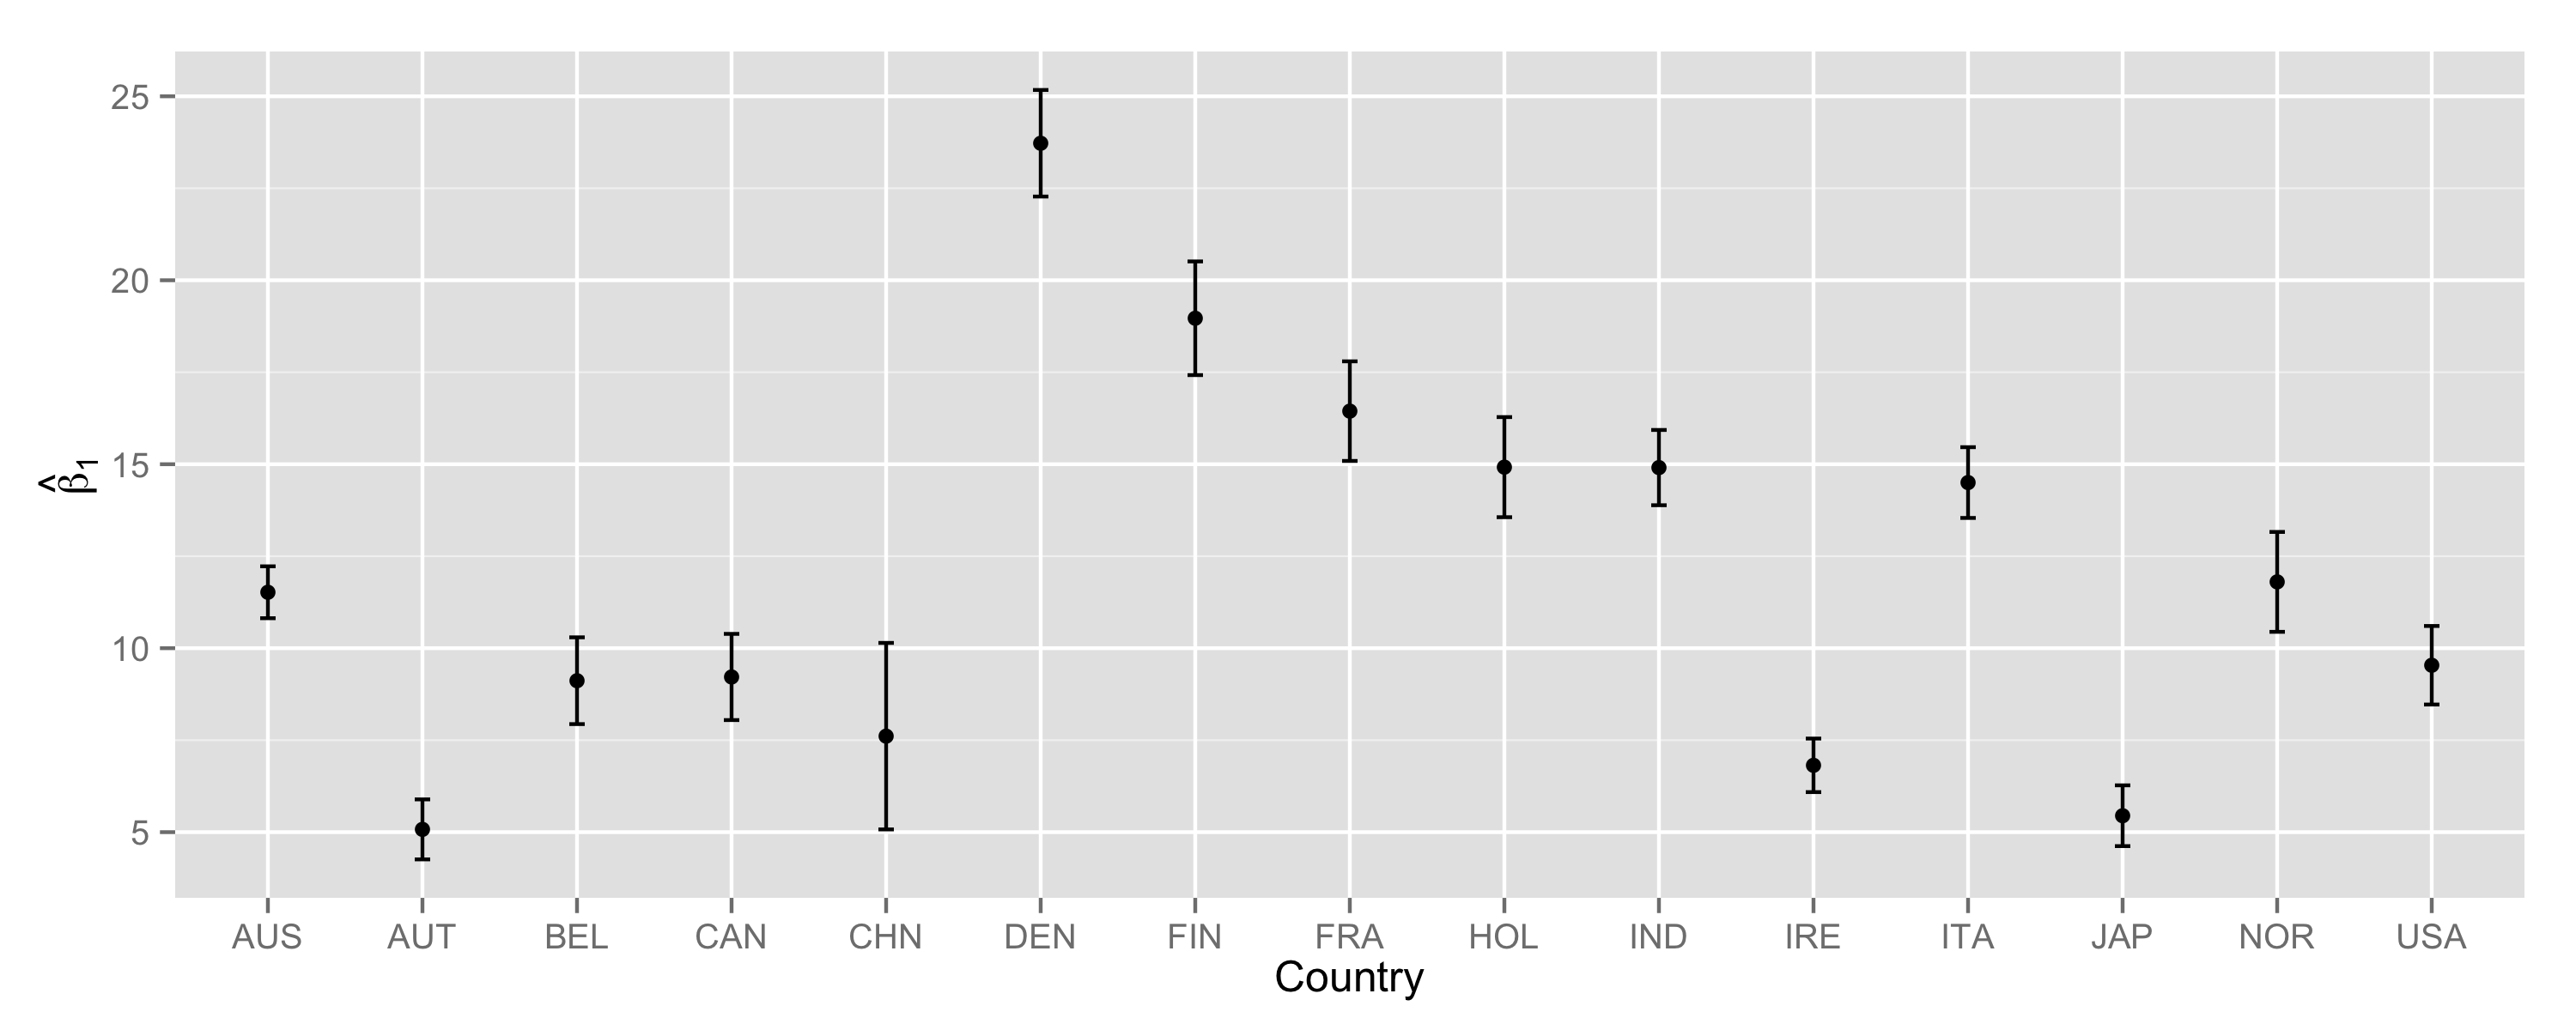
\includegraphics[width=16cm]{b_1_plot} \\
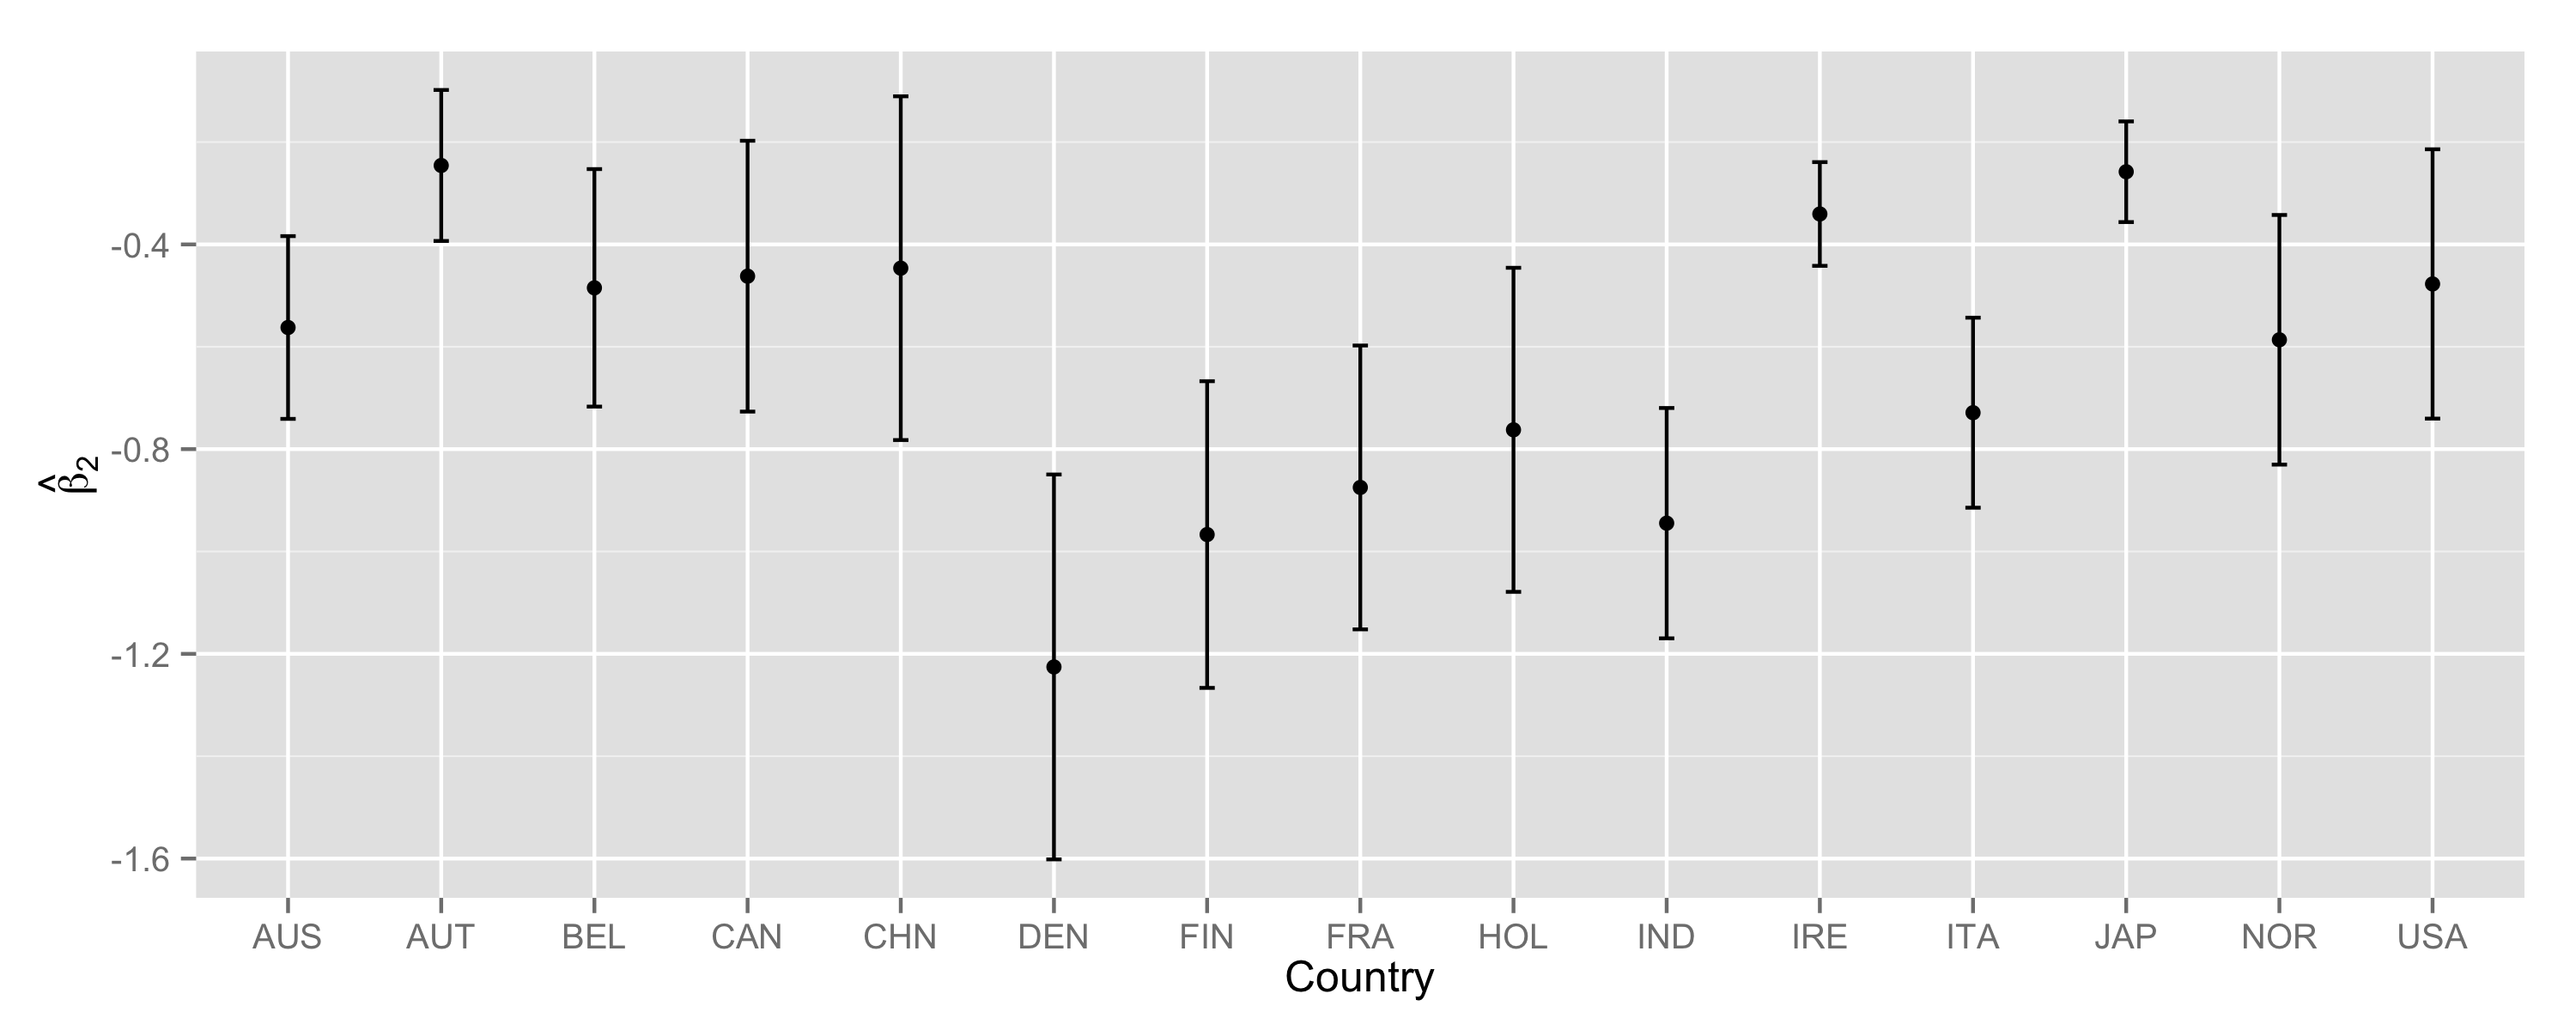
\includegraphics[width=16cm]{b_2_plot} \\
\end{tabular}
}
\end{table}

Table \ref{beta1_est} and \ref{beta2_est} report the estimates and 95\% confidence intervals of parameters $\beta_{1}$ and $\beta_{2}$, and Table \ref{beta12_plot} presents the plots of the results. For the parameter $\beta_{1}$, we can not find any group with more than four groups of countries whose confidence intervals overlap. Such result is consistent with that of \cite{piaggiopadilla2010}. However, for the parameter $\hat{\beta}_{2n}$, among the 15 countries, we can find group of 11 countries whose confidence intervals overlap. Hence, the homogeneity of parameters can not be rejected as in \cite{piaggiopadilla2010}. There are two main reasons for the  differences between our results and theirs. Firstly, they assume the innovation is i.i.d. normally distributed while we allow the error to be serially correlated with itself. Secondly, we incorporate the effect of endogeneity in our limit distribution of estimator. Based on (\ref{example.eqn1}), both reasons will make the critical values and confidence intervals significantly larger than that of \cite{piaggiopadilla2010}.


%%%%%%%%%%%%%%%%%%%%%%%%%%%%%%%%%%%%%%
%                                    %
%                                    %
%            Conclusion              %
%                                    %
%                                    %
%%%%%%%%%%%%%%%%%%%%%%%%%%%%%%%%%%%%%%

\section{Conclusion and discussion} \la{sec:6:conclusion}

In this paper, we establish an asymptotic theory for a nonlinear parametric cointegrating regression model. A general framework is developed for establishing the weak consistency of the NLS estimator $\hat{\theta}_n$. The framework can easily be applied to a wide class of nonstationary regressors, including the partial sum of linear processes and Harris recurrent Markov chains. Limit distribution of $\hat{\theta}_n$ is also established, which  extends previous works. Furthermore, we introduce endogeneity to our model by allowing the error term to be serially dependent on itself, and cross-dependent on the regressor. We show that the limit distribution of $\hat{\theta}_n$ under the endogeneity situation is different from that with martingale error structure. This result is of interest in the applied econometric research area. 

Asymptotics in this paper are limited to univariate regressors and 
nonlinear parametric cointegrating regression models. Specification of the nonlinear regression function $f$ depends usually on the underlying theories of the subject. Illustration can be found in  \cite{baekakkarogaki2004}, where  the concept of the money in the utility function with the constant elasticity of substitution (MUFCES) is used  to relate the money balance with nominal interest rate by the link function $f(x, \al, \beta) = \al + \beta \log(\frac{x}{1 + x})$. More currently, nonparametric method
 has been developed to test the specification of $f$. See, e.g., \cite{wangphillips2012},  for instance.
Extension to multivariate regressors require substantial different techniques. This is because  local time theory can not in general be extended to multivariate data, in which the techniques play a key rule in  the asymptotics of the NLS estimator with nonstationary regressor when $f$ is an integrable function.   Possible extension to multivariate regressors is the index model discussed in \cite{changpark2003}. This again requires some new techniques, and hence we leave it for future  work.


%%%%%%%%%%%%%%%%%%%%%%%%%%%%%%%%%%%%%%
%                                    %
%                                    %
%       Proofs of main results       %
%                                    %
%                                    %
%%%%%%%%%%%%%%%%%%%%%%%%%%%%%%%%%%%%%%

\section{Proofs of main results} \la{sec:6:proof}

This section provides proofs of the main results. We start with some preliminaries, which list the limit theorems that are commonly used in the proofs of the main results.

\subsection{Preliminaries}

Denote $\mathcal N_{\de}(\theta_0) = \{ \theta: \| \theta - \theta_0\| < \de\}$, where $\theta_0 \in \Theta$ is fixed.
\begin{lem} \la{lemClose} Let Assumption \ref{assumpClose} hold. Then, for any $x_t$ satisfying   (\ref {20}) with $T$ being given as in Assumption \ref{assumpClose},
\be \la{lemClose.eqn0}
\sup_{\theta \in \mathcal N_{\de}(\theta_0)} \kappa_n^{-2} \sum_{t = 1}^n \big(|f(x_t, \theta) - f(x_t, \theta_0)| + |f(x_t, \theta) - f(x_t, \theta_0)|^2\big)  &\to_P& 0,
\ee
as $n\to\infty$ first and then $\de \to 0$. If in addition Assumption \ref{assumpMartingale}, then
\be
\kappa_n^{-2} \sum_{t = 1}^n [f(x_t, \theta_0) - f(x_t, \pi_0)]\, u_t   \to_P 0, \la {98}
\ee
for any $\theta_0,\pi_0\in \Theta$, and
\be
\la{lemClose.eqn1}
\sup_{\theta \in \mathcal N_{\de}(\theta_0)}  \kappa_n^{-2} \sum_{t = 1}^n |f(x_t, \theta) - f(x_t, \theta_0)|\, |u_t|  \to_P 0,
\ee
as $n\to\infty$ first and then $\de \to 0$.
\end{lem}

\begin{proof} (\ref {lemClose.eqn0}) is simple.
As $\kappa_n^{-2} \sum_{t = 1}^n [f(x_t, \theta_0) - f(x_t, \pi_0)]^2\le C\kappa_n^{-2} \sum_{t = 1}^n T^2(x_t)=O_P(1)$,
(\ref {98}) follows from Lemma 2 of \cite{laiwei1982}. As for (\ref {lemClose.eqn1}), the result follows from
\bestar
\sum_{t = 1}^n |f(x_t, \theta) - f(x_t, \theta_0)|\, |u_t| \le h(\|\theta-\theta_0\|)\sum_{t = 1}^n T(x_t)\, |u_t|,
\eestar
and $\sum_{t = 1}^n T(x_t)\, |u_t|\le C\sum_{t = 1}^n T(x_t)+
\sum_{t = 1}^n T(x_t)\,\big[ |u_t|-E(|u_t|\mid {\cal F}_{t-1})\big] =O_P(\kappa_n^{2})$.
\end{proof}





\begin{lem} \la{lemJoint} Let Assumption \ref{ad1} (i) hold.
 For any bounded $g (x)$ satisfying  $\int_{-\infty}^{\infty} |g(x)| dx < \infty$, we have
\be
\sum_{t = 1}^n g(x_t) &=& O_P(n/d_n). \la {tya}
\ee
If in addition Assumption \ref{ad1} (ii)--(iii), then, for any bounded $g_i(x), i=1,2,$
satisfying $\int_{-\infty}^{\infty} |g_i(x)| dx < \infty$ and $\int_{-\infty}^{\infty} g_i(x) dx  \ne 0$,
\be \la{lemJoint.eqn1}
\Big \{ \big(\frac {d_n}n\big)^{1/2}\sum_{t=1}^n g_1(x_t) u_t ,\, \frac {d_n}n\sum_{t=1}^n g_2(x_t) \Big \} &\rightarrow_D& \Big \{\tau_1 \, N \, L^{1/2}_{G}(1,0), \tau_2\, L_{G}(1,0) \Big \},
\ee
 where $\tau_1^2 = \int_{-\infty}^{\infty} g_1^2(s) ds$, $\tau_2= \int_{-\infty}^{\infty} g_2(s) ds$ and $N$ is a standard normal variate independent of $G(t)$.
\end{lem}

\begin{proof} For (\ref {tya}),  see Lemma 3.2 of \cite{wangphillips2009}.
Theorem 2.2 of \cite{wang2011} provides  (\ref {lemJoint.eqn1}) with $g_2(x)=g_1^2(x)$. It is not difficult to see that (\ref {lemJoint.eqn1}) still holds for general $g_2(x)$. We omit the details.
\end{proof}



\begin{lem} \la{lemMarkov} Let Assumption \ref {ad1}*(i) hold. For any $g$ such that $\int_{-\infty}^{\infty} |g(x)| \pi(dx) < \infty$ and $\int_{-\infty}^{\infty} g(x) \pi(dx) \ne 0$, we have
\be
\sum_{t = 1}^n g(x_t) &=& O_P[a(n)], \quad
\big [\sum_{t = 1}^n g(x_t)\big ]^{-1} = O_P[a(n)^{-1}]. \la {ty}
\ee
If in addition Assumption \ref{ad1}* (ii)--(iii), then, for any bounded $g_i(x), i=1,2,$ satisfying $\int_{-\infty}^{\infty} |g_i(x)| \pi(dx) < \infty$ and $\int_{-\infty}^{\infty} g_i(x) \pi(dx)  \ne 0$,
\be \la{lemMarkov.eqn2}
\Big \{ a(n)^{-1/2}\sum_{t=1}^n g_1(x_t) u_t ,\, a(n)^{-1}\sum_{t=1}^n g_2(x_t) \Big \}  \rightarrow_D   \Big \{\tau_5 \, N \, \Pi^{1/2}_{\beta}, \tau_6\,\Pi_\beta \Big \},
\ee
 where $\tau_5^2 = \int_{-\infty}^{\infty} g_1^2(s) \pi(ds)$, $\tau_6= \int_{-\infty}^{\infty} g_2(s) \pi(ds)$, $\Pi_{\beta}$ is defined as in Theorem \ref {thmIntegrablelimit1} and $N$ is a standard normal variate independent of $\Pi_\beta$.
\end{lem}


\begin{proof}
The proof of (\ref {ty}) sees Theorem 2.1 of \cite{chen1999}. To prove (\ref{lemMarkov.eqn2}), we first impose an additional assumption that $g_2(x) = g_1^2(x)$. Denote
\be
\Delta^2_n = a(n)^{-1}\sum_{t = 1}^n g_1^2(x_t), \quad Z_{nt} = a(n)^{-1/2}g_1(x_t) \Delta_n^{-1}, \quad  \mbox{and} \quad W_n = \sum_{t = 1}^n Z_{nt} u_k.
\ee
Recalling that $E(u_t|\F_{nt}) = 0$, it is readily seen that given $\{x_1, ..., x_n\}$, $\{Z_{nt} u_t, \F_{nt}\}_{t = 1}^n$ forms a martingale difference sequence. The result (\ref{lemMarkov.eqn2}) will follow if we prove,
\be \la{prfMarkov.eqn1}
\sup_{x} \big | P\big ( W_n \le x \, | \, x_1, ..., x_n \big ) - \Phi(x) \big | \to_P 0.
\ee
%\begin{align}
%\sum_{t = 1}^n |Z_{nt}|^q &\to_P 0, \\
%\sum_{t = 1}^{\tau_n(t)} Z_{nt}^2 \,E(u_t^2 | \F_{nt}) &\to_P t,
%\end{align}
%for all $t \in [0, 1]$.

\noindent Indeed, by noting that $\Delta_n^2$ is measurable with respect to $\si(x_1,...x_n)$, we have, for any $\al, \gamma \in R$,
\begin{align}
&\big |E \big [ e^{i  \al  W_n + i \beta \Delta_n^2} \big ] - e^{-\frac{1}{2} \al^2 } \, E\big [e^{i \beta \tau_5 \Pi_\gamma} \big ] \big| \no\\
&\le E \Big |E \big ( e^{i \al W_n } |\, x_1, ..., x_n \big ) - e^{-\frac{1}{2}\al^2 } \,  \Big| +e^{-\frac{1}{2}\al^2}\Big| Ee^{i \gamma \Delta_n^2} - Ee^{i \gamma \tau_5 \Pi_\beta} \Big | \to 0, \no
\end{align}
by dominated convergence theorem, due to (\ref{prfMarkov.eqn1}) and $\Delta_n^2 \to_D \tau_5 \Pi_\beta$ (see, e.g., Theorem 2.3 of \cite{chen1999}). This implies that
\bestar
\{ W_n, \Delta_n^2 \} \to_D \{N, \tau_5\Pi_\beta\},
\eestar
where $N$ is a standard normal random variable independent of $\Pi_\beta$. Hence, by continuous mapping theorem, we have
\bestar
\Big \{ a(n)^{-1/2}\sum_{t=1}^n g_1(x_t) u_t ,\, a(n)^{-1}\sum_{t=1}^n g_1^2(x_t) \Big \} = \Big \{ \Delta_n W_n, \Delta_n^2\Big \}\to_D \{\tau_5^{1/2} N\Pi_\beta^{1/2}, \tau_5\Pi_\beta\},
\eestar
which implies the required (\ref{lemMarkov.eqn2}).

We now prove (\ref{prfMarkov.eqn1}). By Theorem 3.9 ((3.75) there) in \cite{hallheyde1980} with $\de = q/2 - 1$ that
\bestar
\sup_{x} \big | P\big ( W_n \le x \, | \, x_1, ..., x_n \big ) - \Phi(x) \big | \le A(\de) \mathcal L_n^{1 / (1 + q)}  \quad a.s.,
\eestar
where $A(\de)$ is a constant depending only on $\de$ and $q > 2$, and (set $\F^*_n = \si(x_1, ..., x_n)$)
\bestar
\mathcal L_n = \Delta_n^{-q} \sum_{k = 1}^n |Z_{nk}|^q E(|u_k|^q | \F^*_{n}) + E \Big [ \big | \Delta_n^{-2} \sum_{k = 1}^n Z_{nk}^2 [E(u_k^2 | \F_{nk}) - 1] \big|^{q/2} \Big | \, \F^*_{n} \Big].
\eestar
Recall from Assumption \ref{ad2} (iv) and the fact that $\Delta_n^2 = \sum_{k = 1}^n Z^2_{nk}$, we have,
\bestar
E \Big [ \big | \Delta_n^{-2} \sum_{k = 1}^n Z_{nk}^2 [E(u_k^2 | \F_{nk}) - 1] \big|^{q/2} \Big | \, \F^*_{n} \Big] \to_P 0,
\eestar
by dominated convergence theorem. Hence,  routine calculations show that
\bestar
\mathcal L_n \le C\,\Delta_n^{-(q-2)} \,a(n)^{-(q-2)/2} + o_P(1) = o_P(1),
\eestar
because $\Delta_n^{-2}=O_P(1)$ by (\ref{ty}) and $q > 2$. This proves (\ref{prfMarkov.eqn1}), which implies that (\ref{lemMarkov.eqn2}) holds true with $g_2(x) = g_1^2(x)$. Finally, note that, for any $a$, $b \in R$,
\bestar
a(n)^{-1} \sum_{t = 1}^n \big \{ a g_1^2(x_t) + bg_2(x_t)\big  \}  \to_D  \int_{-\infty}^{\infty} \big [a g_1^2(s) + bg_2(s) \big ] \pi(ds)\, \Pi_\beta,
\eestar
due to Theorem 2.3 of \cite{chen1999}, which implies that
\bestar
\Big \{ a(n)^{-1}\sum_{t=1}^n g_1^2(x_t) ,\, a(n)^{-1}\sum_{t=1}^n g_2(x_t) \Big \}\to_D  \Big \{\int_{-\infty}^{\infty} g_1^2(s) \pi(ds)\, \Pi_\beta, \int_{-\infty}^{\infty} g_2(s) \pi(ds)\, \Pi_\beta, \Big \}.
\eestar
Hence, by continuous mapping theorem,
\bestar
\frac{ \sum_{t=1}^n g_1^2(x_t) }{\sum_{t=1}^n g_2(x_t)} \to_P \int_{-\infty}^{\infty} g_1^2(s)\,  \pi(ds) \Big /  \int_{-\infty}^{\infty} g_2(s) \, \pi(ds) .
\eestar
This shows that (\ref{lemMarkov.eqn2}) is still true with general $g_2(x)$.
\end{proof}


\begin{lem} \la{lemLagJoint} Under Assumption \ref {4.1}, for any bounded $g_i(x), i=1,2,$
satisfying $\int_{-\infty}^{\infty} |g_i(x)|dx < \infty$ and $\int_{-\infty}^{\infty} g_i(x) dx  \ne 0$, we have
\be \la{lemLagJoint.eqn1}
 \sum_{t = 1}^n g_1(x_t) |u_t| = O_P(n / d_n),
\ee
and
\be \la{lemLagJoint.eqn2}
&\Big \{ (n/d_n)^{-1/2}\sum_{t=1}^n g_1(x_t) u_t ,\, (n/d_n)^{-1}\sum_{t=1}^n g_2(x_t) \Big \} \no\\
&\quad \rightarrow_D \Big \{\tau_3 \, N \, L^{1/2}_{G}(1,0), \tau_4 L_{G}(1,0) \Big \},
\ee
 where $\tau_3^2 = (2\pi)^{-1}\int_{-\infty}^{\infty}\hat{g}_1(\mu)^2 [ Eu_0^2 + 2 \sum_{r = 1}^{\infty}E(u_0u_r e^{-i\mu x_r})]\,d\mu$, $\hat{g}_1(\mu)=\int_{-\infty}^{\infty}e^{i\mu x}g_1(x) dx$ and $\tau_4 = \int_{-\infty}^{\infty} g_2(s) ds$.
\end{lem}

\begin{proof}
See Theorem 3 and 5 of \cite{jaganathan2008}.
\end{proof}

\begin{lem} \la{lemEndo} Under Assumption \ref{4.2}, for any twice continuous differentiable function $g_i(x)$, $i = 1, 2$, satisfying $|g_i'(x)| \le K (1 + |x|^{\al})$ for some constants $K, \al > 0$ for all $x \in R$, and if $q \ge \max(3, 2\al)$ where $q$ is given Assumption \ref{4.2}, we have
\begin{align} \la{lemEndo.eqn1}
&\Big \{ \frac{1}{\sqrt{n}} \sum_{t = 1}^{n} g_1 \Big ( \frac{x_t}{\sqrt{n}}\Big) u_t, \frac{1}{n} \sum_{t = 1}^{n} g_2  \Big ( \frac{x_t}{\sqrt{n}}\Big) \Big \} \no\\
&\to_D \Big \{ \sigma_{\xi u} \int_{0}^{1} g_1'(W(t))dt + \int_0^1 g_1(W(t)) dU(t), \int_0^1 g_2(W(t)) dt\Big \},
\end{align}
as $n \to \infty$, where $\si_{\xi u} = \sum_{j = 0}^{\infty} E( \xi_0 u_j)$, and $(W(t), U(t))$ is a bivariate Brownian motion with covariance matrix
\bestar
\Delta = \begin{pmatrix}
\phi^2 E\ep_0^2 & \phi \psi E \ep_0 \nu_0 \\
\phi\psi E \ep_0 \nu_0 & \psi^2 E\nu_0^2
\end{pmatrix}.
\eestar
\end{lem}
\begin{proof} See Theorem 4.3 of \cite{ibragimovphillips2008} with minor improvements.
We omit the details.
\end{proof}

\begin{lem} \la{lemC}
Under Assumptions \ref{ad1}(i) and  \ref {ad2},   we have
\be \la{lemC.eqn1}
\frac {d_n}n\,\sup_{\theta \in \mathcal N_{\de}(\theta_0)}
\sum_{t = 1}^n \big|\dot f_i(x_t, \theta)\,\dot f_j(x_t, \theta) - \dot f_i(x_t, \theta_0)\,\dot f_j(x_t, \theta_0)\big|  &\to_P& 0, \\
\frac {d_n}n\,\sup_{\theta \in \mathcal N_{\de}(\theta_0)}\la{lemC.eqn2}
\sum_{t = 1}^n \big|\ddot f_{ij}(x_t, \theta)\,[ f(x_t, \theta) -  f(x_t, \theta_0)]\big|  &\to_P& 0,
\ee
as $n\to\infty$ first and then $\de \to 0$,  for any $1\le i, j\le m$. If in addition Assumption \ref{ad1} (ii)--(iii), then
\be\la{lemC.eqn3}
\frac {d_n}n\,\sup_{\theta \in \mathcal N_{\de}(\theta_0)}\big| \sum_{t = 1}^n\ddot f_{ij}(x_t, \theta)\,u_t \big| \to_P 0,
\ee
as $n\to\infty$ first and then $\de \to 0$,  for any $1\le i, j\le m$.

Similarly, under Assumptions \ref{ad1}* (i) and  \ref {ad2}*,
(\ref {lemC.eqn1}) and (\ref {lemC.eqn2}) are  true if we replace $d_n / n$ by $a(n)^{-1}$. If in addition Assumption \ref{ad1}* (ii) and (iii), then (\ref {lemC.eqn3})
 holds if we replace $d_n / n$ by $a(n)^{-1}$.
\end{lem}


\begin{proof} We only prove (\ref{lemC.eqn1}). Others are similar and the details are omitted. First note that, by Assumption \ref{ad2} (i) and (iii),
\begin{align}
\sup_{\theta \in \Theta} |f_i(x_t, \theta)| &\le \sup_{\theta \in \Theta} |\dot{f}_i(x_t, \theta)-\dot{f}_i(x_t, \theta_0)| + |\dot{f}_i(x_t, \theta_0)| \no\\
 &\le \sup_{\theta \in \Theta} h(\| \theta - \theta_0\|)T(x_t) + |\dot{f}_i(x_t, \theta_0)| \le C. \no
\end{align}
It follows that
\bestar
&& \big|\dot f_i(x_t, \theta)\,\dot f_j(x_t, \theta) - \dot f_i(x_t, \theta_0)\,\dot f_j(x_t, \theta_0)\big| \no\\
&\le& \big|\dot f_i(x_t, \theta) \big |\big|\dot f_j(x_t, \theta)- \dot f_j(x_t, \theta_0)\big| + \big|\dot f_j(x_t, \theta_0) \big |\big|\dot f_i(x_t, \theta) - \dot f_i(x_t, \theta_0)\big| \no\\
&\le& C\big|\dot f_j(x_t, \theta)- \dot f_j(x_t, \theta_0)\big| +C_1\big|\dot f_i(x_t, \theta) - \dot f_i(x_t, \theta_0)\big|.
\eestar
Therefore, by recalling (\ref {tya}), the result (\ref{lemC.eqn1}) follows
from an application of Lemma \ref{lemClose} with $\kappa_n^2=n/d_n$.
\end{proof}

\begin{lem}  \la{lemHomoC}
 Under Assumptions \ref{assumpLimitHomo1} and \ref{assumpLimitHomo2},   we have
\be \la{lemC.eqn1a}
\frac {1}{n\dot v_i (d_n)\dot v_j (d_n)}\,\sup_{\theta \in \mathcal N_{\de}(\theta_0)}
\sum_{t = 1}^n \big|\dot f_i(x_t, \theta)\,\dot f_j(x_t, \theta) - \dot f_i(x_t, \theta_0)\,\dot f_j(x_t, \theta_0)\big|  &\to_P& 0, \\
\frac {1}{nv(d_n)\ddot v_{ij} (d_n)}\,\sup_{\theta \in \mathcal N_{\de}(\theta_0)}\la{lemC.eqn2a}
\sum_{t = 1}^n \big|\ddot f_{ij}(x_t, \theta)\,[ f(x_t, \theta) -  f(x_t, \theta_0)]\big|  &\to_P& 0,\\
\la{lemC.eqn3a}
\frac {1}{n\ddot v_{ij} (d_n)}\,\sup_{\theta \in \mathcal N_{\de}(\theta_0)}\big| \sum_{t = 1}^n\ddot f_{ij}(x_t, \theta)\,u_t \big| &\to_P& 0,
\ee
as $n\to\infty$ first and then $\de \to 0$,  for any $1\le i, j\le m$.
\end{lem}

\begin{proof}  Recall $\max_{1\le t\le n}|x_t|/d_n=O_P(1)$. Without loss of generality, we assume $\max_{1\le t\le n}|x_t|/d_n\le K_0$ for some $K_0>0$.
It follows from Assumption \ref {assumpLimitHomo2} and $d_n \to \infty$  that, for any $1\le i\le m$ and $\theta\in \Theta$,
\bestar
\big|\dot f_i(x_t, \theta)\big| &\le& \dot v_i (d_n)\big( |\dot h_i(x_t/d_n)|+o(1)\, T_{1\dot f_i}(x_t/d_n) \big),\\
\big|\dot f_i(x_t, \theta) - \dot f_i(x_t, \theta_0)\big| &\le& A_{\dot f_i}(||\theta-\theta_0||)\dot v_i (d_n) T_{1\dot f_i}(x_t/d_n).
\eestar
This implies that
\be
&& \sup_{\theta \in \mathcal N_{\de}(\theta_0)}
\sum_{t = 1}^n \big|\dot f_i(x_t, \theta)\,\dot f_j(x_t, \theta) - \dot f_i(x_t, \theta_0)\,\dot f_j(x_t, \theta_0)\big| \no\\
&\le&2\, (A_{\dot f_i}(\delta)+A_{\dot f_j}(\delta))\, \dot v_i (d_n)\dot v_j (d_n)\, \sum_{t = 1}^n\big( |\dot h_i(x_t/d_n)|+ T_{1\dot f_i}(x_t/d_n) \big).\la{lemHomoC.eqn1}
\ee
(\ref {lemC.eqn1a}) now follows from $A_{\dot f_i}(\delta)\to 0$ as $\delta\to 0$ and
\bestar
\frac 1n\sum_{t = 1}^n\big[ |\dot h_i(x_t/d_n)|+ T_{1\dot f_i}(x_t/d_n) \big]\to_D \int_0^1\big[ |\dot h_i(G(t))|+ T_{1\dot f_i}(G(t))\big] dt=O_P(1),
\eestar
due to Assumptions \ref{assumpLimitHomo1} (iii) and 3.4 (iii).

The proof of (\ref {lemC.eqn2a}) is similar and hence the details are omitted. As for (\ref {lemC.eqn3a}), by noting
\bestar
\big| \sum_{t = 1}^n\ddot f_{ij}(x_t, \theta)\,u_t \big|\le \big| \sum_{t = 1}^n\ddot f_{ij}(x_t, \theta_0)\,u_t \big|+ \sum_{t = 1}^n|\ddot f_{ij}(x_t, \theta)-\ddot f_{ij}(x_t, \theta_0)|\,|u_t|,
\eestar
the result can be proved by using the similar arguments as in (\ref {98}) and (\ref {lemClose.eqn1}) of Lemma \ref {lemClose}.
\end{proof}

\begin{lem} \la{lemad}  Let Assumption \ref{assumpLimitHomo1} hold. Then, for any regular functions $g(x, \theta)$ and $g_1(x, \theta)$ on $\Theta$, we have
\be
&& \Big\{\frac 1{\sqrt n}\sum_{t=1}^ng\Big (\frac {x_t}{d_n}, \theta\Big )\, u_t,\ \frac 1{ n}\sum_{t=1}^ng_1\Big (\frac {x_t}{d_n}, \theta\Big)\Big\} \no\\
&&\qquad \to_D\ \Big\{\int_0^1 g\big(G(t), \theta\big)dU(t),\ \int_0^1 g_1\big(G(t), \theta\big)dt\Big\}.
\ee
\end{lem}

\begin{proof} If $g(x, \theta)$ and $g_1(x, \theta)$ are continuous functions, the result follows from (\ref {nm1}) and the continuous mapping theorem. See, \cite{kurtzprotter1991} for instance. The extension from continuous function to regular function is standard in literature. The details can be found in PP or \cite{parkphillips1999}.
\end{proof}

\begin{lem} \la{lemWu} Let $D_n(\theta, \theta_0) =  Q_n(\theta) - Q_n(\theta_0)$.
 Suppose that, for any $\de > 0$,
\be \la{lemWu.eqn1}
\liminf_{n \to \infty} \inf_{|\theta - \theta_0| \ge \delta} D_n(\theta, \theta_0) > 0 \quad in \quad  probability,
\ee
 then $\hat{\theta}_n \rightarrow_P \theta_0$.
\end{lem}

\begin{proof}
See Lemma 1 of \cite{wu1981}.
\end{proof}



\subsection{Proof of Theorems}

\begin{proof}[Proof of Theorem \ref {thmConsistency}]
Let $\mathcal N$ be any open subset of $\Theta$ containing $\theta_0$. Since $\hat{\theta}_n$ is the minimizer of $Q_n(\theta)$ over $\theta \in \Theta$,  by Lemma \ref{lemWu}, proving consistency is equivalent to showing that, for any $0<\eta<1$ and $\theta \ne \theta_0$, where $\theta, \theta_0\in \Theta$, there exist
 $n_0 > 0$ and $M_1>0$ such that
\be \la{prfConsistency.eqn1}
P \Big ( \inf_{\theta \in \Theta \cap \mathcal N^c}\, D_n(\theta, \theta_0) \ge  \kappa^2_n /M_1 \Big ) \ge 1 - \eta,
\ee
for all $n > n_0$.

Denote $\mathcal N_{\de}(\pi_0) = \{ \theta: \| \theta - \pi_0\| < \de\}$. Note that $\Theta \cap \mathcal N^c$ is compact, by the finite covering property of compact set, (\ref{prfConsistency.eqn1}) will follow if we prove that, for any fixed $\pi_0 \in \Theta \cap \mathcal N^c$,
\be \la{prfConsistency.eqn2}
\sup_{\theta \in \mathcal N_{\de}(\pi_0)} \kappa_n^{-2} \Big | D_n(\theta, \theta_0) - D_n(\pi_0, \theta_0) \Big | \to_P 0,
\ee
as $n\to\infty$ first and then $\de \to 0$, and for $\forall \ep>0$, there exists $M_1 > 0$ and $n > n_0$ such that for all $n > n_0$,
\be \la{prfConsistency.eqn3}
P\Big ( D_n(\pi_0, \theta_0) \ge \kappa^2_n/M_1 \Big ) \ge 1 -2 \eta.
\ee
The result  (\ref{prfConsistency.eqn2}) is simple. Indeed, by Lemma \ref{lemClose},  for each fixed $\pi_0 \in \Theta \cap \mathcal N^c$, we have
\begin{align}
&\sup_{\theta \in \mathcal N_{\de}(\pi_0)}\kappa_n^{-2}\Big | D_n(\theta, \theta_0) - D_n(\pi_0, \theta_0) \Big | \no\\
&\le \sup_{\theta \in \mathcal N_{\de}(\pi_0)} \kappa_n^{-2}\sum_{t=1}^n (f(x_t, \theta) - f(x_t, \pi_0))^2 \no\\
&\hskip 3.5cm + \sup_{\theta \in \mathcal N_{\de}(\pi_0)}\kappa_n^{-2} \sum_{t = 1}^n |f(x_t, \theta) - f(x_t, \pi_0)|| u_t|\no\\
&\to_P 0,
\end{align}
as $n\to\infty$ first and then $\de \to 0$, which yields (\ref {prfConsistency.eqn2}).

To prove (\ref{prfConsistency.eqn3}), we  recall
\bestar
D_n(\pi_0, \theta_0) =  \sum_{t = 1}^n (f(x_t, \pi_0) - f(x_t, \theta_0))^2 -  \sum_{t = 1}^n (f(x_t, \pi_0) - f(x_t, \theta_0)) u_t.
\eestar
This, together with (\ref {21}) and (\ref {98}), implies that,
 for any $\eta>0$, there exists $n_0 > 0$ and $M_1 > 0$ such that for all $n > n_0$,
\begin{align}
P\Big ( D_n(\pi_0, \theta_0) \ge \kappa^2_n M_1^{-1} \Big ) &\ge P \Big ( \sum_{t = 1}^n ( f(x_t, \pi_0) - f(x_t, \theta_0))^2 \ge \kappa^2_n\, M_1^{-1}/2 \Big ) - \eta \no\\
&\ge1 -2 \eta, \no
\end{align}
which implies (\ref{prfConsistency.eqn3}).

Finally, by noting $Q_n(\theta_0) = n^{-1} \sum_{t = 1}^n u_t^2 \to_P \si^2$ due to  Assumption \ref{assumpMartingale} and strong law of large number,  it  follows from the consistency of $\hat{\theta}_n$ and (\ref{prfConsistency.eqn2}) that
\bestar
|\hat{\si}_n^2 - \si^2| \le C \kappa_n^{-2} |Q_n(\hat{\theta}_n) - Q_n(\theta_0)| + o_P(1) = o_P(1).
\eestar
\end{proof}


\begin{proof}[Proof of Theorem \ref {thmLinearConsistency}]
(\ref {20}) follows from (\ref {tya}) of Lemma \ref{lemJoint}.
(\ref {21}) follows from (\ref {lemJoint.eqn1}) of Lemma \ref{lemJoint} with $g_2(x)=(f(x, \theta)-f(x, \theta_0))^2$ and the facts that $P(L_G(1,0) > 0) = 1$ and $\int_{-\infty}^{\infty} (f(s, \theta) - f(s, \theta_0))^2 ds > 0$, for any $\theta \ne \theta_0$.
\end{proof}


\begin{proof}[Proof of Theorem \ref {thmMarkovConsistency}]
 (\ref {20}) follows from (\ref {ty}) of  Lemma \ref{lemMarkov} with $g(x)=T(x)+T^2(x)$.
  (\ref {21}) follows from (\ref {lemMarkov.eqn2}) of Lemma \ref{lemMarkov} with   $g_2(x)=(f(x, \theta)-f(x, \theta_0))^2$ and the facts that
   $P(\Pi_{\beta}> 0) = 1$ and $\int_{-\infty}^{\infty} (f(s, \theta) - f(s, \theta_0))^2 \pi(ds) > 0$, for any $\theta \ne \theta_0$.
\end{proof}

\begin{proof}[Proof of Theorem \ref {thmHomoConsistency}]
Recalling $T(\lam x)\le v(\lam)\, T_1(x)$,  we have
\be
\frac{1}{nv^2(d_n)} \sum_{t = 1}^n [T(x_t) + T^2(x_t)] &\le& \frac{1}{n} \sum_{t = 1}^n \big [T_1\Big (\frac{x_{t}}{ d_n}  \Big) + T_1^2\Big (\frac{x_{t} }{d_n}  \Big) \big ]\no\\
&\to_D&\int_0^1[T_1(G(t))+T_1^2(G(t))]dt, \la {101}
\ee
where the convergence in distribution comes from \cite{berkeshorvath2006}.
This proves (4) with $\kappa_n = \sqrt{n}v(d_n) $ due to the local integrability of $T_1+T_1^2$.
To prove (5), by letting $G(\lambda, x) := f(\lambda x, \theta) - f(\lambda x, \theta_0) - v(\lambda) g(x,\theta, \theta_0)$, we have
\begin{align}
&\frac{1}{nv^2(d_n)} \sum_{t = 1}^n ( f(x_t, \theta) - f(x_t, \theta_0))^2  \no\\
&=\frac{1}{nv^2(d_n)} \sum_{t = 1}^n \Big [G\Big (d_n, \frac{x_t}{d_n} \Big ) + v(d_n) g\Big(\frac{x_t}{d_n},\theta, \theta_0\Big)\Big]^2  \no\\
&\ge  \frac{1}{n} \sum_{t = 1}^n g^2\Big(\frac{x_t}{d_n},\theta, \theta_0\Big) - | \Lambda_n |,   \la{prf.HomoConsistency.eqn0}
\end{align}
where $\Lambda_n =  \frac{2}{nv(d_n)}\sum_{t = 1}^n   G\Big (d_n, \frac{x_t}{d_n} \Big ) \,g\Big(\frac{x_t}{d_n},\theta, \theta_0\Big)$.
The similar arguments as in the proof of (\ref {101}) yield that
\be
\frac{1}{n} \sum_{t = 1}^n g^2\Big(\frac{x_t}{d_n},\theta, \theta_0\Big) &\to_D& Z:=\int_0^1g^2(G(s), \theta, \theta_0)ds, \la {102}
\ee
where  $P(0<Z<\infty)=1$ due to  Assumption \ref{assumpClose}* (i). On the other hand, it follows from (10) that
\bestar
\frac{1}{nv^2(d_n)}\sum_{t = 1}^n   G^2\Big (d_n, \frac{x_t}{d_n} \Big ) &\le& \frac {o(1)}{nv^2(d_n)}\sum_{t = 1}^n T^2(x_t) \le \frac {o(1)}{n}\sum_{t = 1}^n T_1^2(x_t/d_n) =o_P(1).
\eestar
Now (5) follows from (\ref{prf.HomoConsistency.eqn0}), (\ref {102}) and the fact that
\bestar
\Lambda_n
 \le 2\Big |  \frac{1}{nv^2(d_n)}\sum_{t = 1}^n   G^2\Big (d_n, \frac{x_t}{d_n} \Big )\Big |^{1/2}\,  \Big |\frac{1}{n}\sum_{t = 1}^n \,g^2\Big(\frac{x_t}{d_n},\theta, \theta_0\Big)  \Big |^{1/2} \to_P 0.
\eestar
\end{proof}


\begin{proof}[Proof of Theorem \ref {thmHomoConsistent1}] Let $\Theta_0 = \{ \| \theta - \theta_0 \| \ge \de \}$ where  $\de>0$ is a constant.
By virtue of Lemma \ref{lemWu},   it suffices to prove that, for any $\eta, M_0 >0$, there exist a $n_0 >0$ such that, for all $n > n_0$,
\be \la{prfHomoConsistent2.eqn1}
P \Big (n^{-1} \inf_{\theta \in \Theta_0} D_n(\theta, \theta_0) > M_0 \Big ) > 1-  \eta.
\ee
To prove (\ref{prfHomoConsistent2.eqn1}),  first note that  $\sum_{t=1}^nu_t^2/n\le M_0$ in probability, for some $M_0>0$, due to the Assumption 2.2 (i). This, together with Cauchy-Schwarz Inequality, yields that
\begin{align}
&n^{-1}D_n(\theta, \theta_0) \no\\
& \quad = \frac{1}{n} \sum_{t = 1}^n (f(x_t, \theta) - f(x_t, \theta_0))^2 - \frac{2}{n} \sum_{t = 1}^n (f(x_t, \theta) - f(x_t, \theta_0))u_t  \no\\
&\quad \ge \frac{1}{n} \sum_{t = 1}^n (f(x_t, \theta) - f(x_t, \theta_0))^2 - \frac{2}{n}\Big ( \sum_{t = 1}^n (f(x_t, \theta) - f(x_t, \theta_0))^2 \Big )^{1/2} \Big (\sum_{t = 1}^n u^2_t \Big )^{1/2}  \no\\
&\quad \ge M_n(\theta, \theta_0)\Big [1  - \frac{2\sqrt{M_0 + o_P(1) }}{M_n(\theta, \theta_0 )^{1/2} } \Big ] ,
\end{align}
where $M_n(\theta, \theta_0)=
 \frac{1}{n} \sum_{t = 1}^n (f(x_t, \theta) - f(x_t, \theta_0))^2$. Hence, for any equivalent process $x_{k}^*$ of $x_k$ (i.e., $x_{k}^*=_D x_{k}, 1\le
k\le n, n\ge 1$, where $=_D$ denotes equivalence in distribution), we have
\be
P \Big (n^{-1} \inf_{\theta \in \Theta_0} D_n(\theta, \theta_0) > M_0 \Big ) \ge
P \Big (\inf_{\theta \in \Theta_0}M_n^*(\theta, \theta_0)\Big [1  - \frac{2\sqrt{M_0 + o_P(1) }}{M_n^*(\theta, \theta_0 )^{1/2} } \Big ] >M_0 \Big ), \la {14}
\ee
where $M_n^*(\theta, \theta_0)= \frac{1}{n} \sum_{t = 1}^n (f(x_t^*, \theta) - f(x_t^*, \theta_0))^2$.

Recalling $x_{[nt]}/d_n \to_D G(t)$ on $D[0,1]$ and
 $G(t)$ is a continuous
Gaussian process, by the so-called
Skorohod-Dudley-Wichura representation theorem (e.g., Shorack and
Wellner, 1986, p. 49, Remark 2), we can choose   an
equivalent process $x_{k}^*$ of $x_k$  so that
\be
\sup_{0\le t\le 1}|x_{[nt]}^*/d_n-G(t)| &=&o_P(1). \la {a17}
\ee
For this equivalent process $x_t^*$, it follows from the structure of $f(x,\theta)$  that
\be \la{190}
m(d_n, \theta)^2 &:=& \frac{1}{n v(d_n, \theta)^2} \sum_{t = 1}^n f(x_t^*, \theta)^2\no\\
&=&\frac{1}{n } \sum_{t = 1}^n h(x_t^*/d_n, \theta)^2 +o_P(1) \no\\
&=&  \int_0^1 h(x_{[ns]}^*/d_n, \theta)^2ds+o_P(1) \no\\
&\to_P& \int_{0}^1 h(G(s), \theta)^2 ds =: m(\theta)^2,
\ee
uniformly in $\theta\in\Theta$. Due to (\ref {190}), the same argument as in the proof of Theorem 4.3 in PP yields that
\bestar
\inf_{\theta \in \Theta_0}M_n^*(\theta, \theta_0) \to \infty, \quad \mbox{in probability,}
\eestar
which, together with (\ref {14}), implies (\ref {prfHomoConsistent2.eqn1}).
\end{proof}


\begin{proof}[Proof of Theorem \ref {th3.1}]
It is readily seen that
\be \la{rmkProofOutline.eqn1}
\dot{Q}_n(\theta_0) &=& - \sum_{t=1}^n \dot{f}(x_t, \theta_0) (y_t - f(x_t, \theta_0)) = - \sum_{t=1}^n \dot{f}(x_t, \theta_0) u_t, \no\\
\ddot{Q}_n(\theta) &=& - \sum_{t=1}^n \dot{f}(x_t, \theta) \dot{f}(x_t, \theta)' - \sum_{t=1}^n \ddot{f}(x_t, \theta)( y_t - f(x_t, \theta)), \no
\ee
 for any $\theta\in \Theta$. It follows from the conditions (i)--(iii) that
 \bestar
 \sup_{\theta:\parallel D_n(\theta-\theta_0)\parallel\le k_n}
\,\parallel (D_n^{-1})'\,\big[\ddot{Q}_n(\theta)-\ddot{Q}_n(\theta_0) \big]\,D_n^{-1}\parallel = o_P(1).
 \eestar
 By using (iii) and (iv), we have
 $
(D_n^{-1})'\, \dot{Q}_n(\theta_0)=O_P(1)$ and $
(D_n^{-1})'\,\ddot{Q}_n(\theta_0) \,D_n^{-1} \to_D M. $
 As $M>0,$ a.s.,  $\lam_{min} [(D_n^{-1})'\,\ddot{Q}_n(\theta_0) \,D_n^{-1}] \ge \eta_n$ with probability that goes to one for some $\eta_n>0$, where
 $\lam_{min}(A)$ denotes the smallest eigenvalue of $A$ and $\eta_n\to 0$
 can be chosen as slowly as required. Due to these facts, a modification of  Lemma 1 in \cite{andrewssun2004} implies (\ref {ad191}). Note that  (iv)' implies (iv).
 The result $D_n(\hat\theta_n-\theta_0)\to_D M^{-1}Z$ follows from (\ref {ad191}) and
 the continuing mapping theorem.
\end{proof}

\begin{proof}[Proof of Theorem \ref {thmIntegrablelimit}]
 It suffices to verify the conditions (i)--(iii) and (iv)' of Theorem \ref {th3.1} with
 \bestar
 D_n =\sqrt {n/d_n}\,  \mbox{{\bf I}}, \quad  Z= \Sigma^{1/2} \, \mbox{{\bf N}}L_G^{1/2}(1,0), \quad M=\Sigma\, L_G(1, 0),
 \eestar
 where {\bf I} is an identity matrix, under Assumptions \ref {ad1} and \ref {ad2}. In fact, as $n/d_n\to\infty$, we may take $k_n\to\infty$
 such that $\theta: ||D_n(\theta-\theta_0)||\le k_n$ falls in $\mathcal N_{\de}(\theta_0) = \{ \theta: || \theta - \theta_0|| < \de\}$.
 This, together with Lemma \ref {lemC}, yields  (i)--(iii).

On the other hand, it follows from Lemma \ref{lemJoint} with $g_1(x)=\al_3'\dot{f}(x, \theta_0)$ and $g_2(x)=\al_1'\dot{f}(x, \theta_0)\,\dot{f}(x, \theta_0)'\al_2 $ that, for any $\al_i=(\al_{i1},...,\al_{im})\in R^m, i=1,2,3,$
\begin{align} \la{prfIntegrablelimit.eqn5}
&\Big \{  \al_3'  \,Z_n, \,  \al_1' Y_n\,\al_2\Big \}\no \\
&= \Big \{ \Big (\frac{d_n}{n}\Big)^{1/2}\,\sum_{t=1}^n \al_3'\, \dot{f}(x_t, \theta_0) u_t ,\,\frac{d_n}{n}\sum_{t=1}^n \al_1'\dot{f}(x_t, \theta_0)\,\dot{f}(x_t, \theta_0)'\al_2  \Big \} \no\\
&\rightarrow_D  \Big \{\tau\,N\, L_G^{1/2}(1, 0), \al_1'\,M\, \al_2\Big \} =_D \Big \{ \al_3' \,Z,\ \al_1'\,M\, \al_2 \Big \},
\end{align}
where $\tau^2 = \int_{-\infty}^{\infty} [\al_3'\dot{f}(s, \theta_0)]^2 ds $, $N$ is a standard normal random variable independent of $G(t)$ and we have used the fact that
\bestar
\tau\, N &=& \Big(\int_{-\infty}^{\infty} [\al_3'\dot{f}(s, \theta_0)]^2 ds\Big)^{1/2}\,  N \no\\
&=_D& \al_3' \Big(\int_{-\infty}^{\infty} \dot{f}(s, \theta_0)\dot{f}(s, \theta_0)' ds\Big)^{1/2}\, \mbox{{\bf N}} =\al_3'\, \Sigma^{1/2}\,\mbox{{\bf N}}.
\eestar
This proves (iv)'.
\end{proof}



\begin{proof}[Proof of Theorem \ref {thmIntegrablelimit1}]
As in the proof of  Theorem \ref{thmIntegrablelimit}, it suffices to verify the conditions (i)--(iii) and (iv)' of Theorem \ref {th3.1} with
\bestar
D_n = a(n)\mbox{{\bf I}}, \quad Z = \Sigma_\pi^{1/2} \, \mbox{{\bf N}}\Pi_\beta, \quad M &=& \Sigma_\pi \, \Pi_\beta, \no
\eestar
under Assumptions \ref {ad1}* and \ref {ad2}*. The details are similar to that of Theorem \ref{thmIntegrablelimit}, with Lemma \ref{lemJoint} replaced by Lemma \ref{lemMarkov}, and hence are omitted.
\end{proof}

\begin{proof}[Proof of Theorem \ref {thmHomoLimit1}]
It suffices to verify the conditions (i)--(iii) and (iv)' of Theorem \ref {th3.1} with $D_n=\mbox{diag} (\sqrt n\dot{v}_1(d_n), ...,\sqrt n\dot{v}_m(d_n))$,
\bestar
 Z =   \int_{0}^{1} \dot{h}(G(t), \theta_0) dU(t),\quad M = \int_{0}^{1}\Psi(t) \Psi(t)' dt,
\eestar
under Assumptions \ref {assumpLimitHomo1} and \ref {assumpLimitHomo2}.
Recalling  $\sup_{1 \le i, j \le m} | \frac{v(d_n)\, \ddot v_{ij}(d_n)}{\dot v_i(d_n)\,  \dot v_j(d_n)}|<\infty$, it follows from (\ref {lemC.eqn2a}) that
\bestar
&& \frac{1}{n\dot{v}_i(d_n) \dot{v}_j(d_n)} \sup_{\theta\in \mathcal N_{\de}(\theta_0) } \,\sum_{t = 1}^n \big | \ddot{f}_{ij}(x_t, \theta) [f(x_t, \theta) - f(x_t, \theta_0)] \big | \no\\
&& \le\frac{C}{n\ddot{v}_{ij}(d_n) v(d_n)}  \sup_{\theta\in \mathcal N_{\de}(\theta_0) }\,\sum_{t = 1}^n \big | \ddot{f}_{ij}(x_t, \theta) [f(x_t, \theta) - f(x_t, \theta_0)] \big | =o_P(1),
\eestar
for any $1 \le i, j\le m$. On the other hand,  as $\sqrt{n}\dot{v}_i(d_n)\to\infty$ for all $1 \le i \le m$, we may take $k_n\to\infty$ such that $\theta: ||D_n(\theta-\theta_0)||\le k_n$ falls in $\mathcal N_{\de}(\theta_0) = \{ \theta: || \theta - \theta_0|| < \de\}$. These facts imply that
$$\sup_{\theta:\parallel D_n(\theta-\theta_0)\parallel\le k_n}\,
 \parallel (D_n^{-1})'\,\sum_{t=1}^n
 \ddot{f}(x_t, \theta)\, \big[f(x_t, \theta)-f(x_t, \theta_0)\big]\,  D_n^{-1}\,\parallel = o_P(1).$$
This proves the required (ii). The proofs of (i) and (iii) are similar, we omit the details. Finally (iv)' follows from Lemma \ref {lemad} with
\begin{equation*}
g(x, \theta_0)=\al_3'\dot{h}(x, \theta_0) \quad \mbox{and} \quad g_1(x, \theta_0)=\al_1'\dot{h}(x, \theta_0) \dot{h}(x, \theta_0)'\al_2.
\end{equation*}
\end{proof}

\begin{proof}[Proof of Theorem \ref {endo11}]
We first establish the consistency result. The proof goes along the same line as in Theorem \ref{thmConsistency}. It suffices to show that for any fixed $\pi_0 \in \Theta \cap \mathcal N^c$,
\be \la{prf11.eqn1}
\sup_{\theta \in \mathcal N_{\de}(\pi_0)} \frac{d_n}{n} \sum_{t = 1}^n |[f(x_t, \theta) - f(x_t, \pi_0)]u_t|  \to_P 0,
\ee
as $\de\to 0$ uniformly for all large $n$, and
\be\la{prf11.eqn2}
\sum_{t = 1}^n (f(x_t, \pi_0) - f(x_t, \theta_0)) u_t = o_P(n/d_n).
\ee

 By (\ref{lemLagJoint.eqn1}) in Lemma \ref{lemLagJoint} with $g_1(x) = |T(x)|$, (\ref{prf11.eqn1}) follows from
\begin{align}
\sup_{\theta \in \mathcal N_{\de}(\pi_0)}\frac{d_n}{n} \sum_{t = 1}^n |[f(x_t, \theta) - f(x_t, \pi_0)]u_t| &\le \sup_{\theta \in \mathcal N_{\de}(\pi_0)} h(\|\theta- \pi_0\|) \,  \frac{d_n}{n} \sum_{t = 1}^n|T(x_t)|| u_t| \no\\
&\le C\, \sup_{\theta \in \mathcal N_{\de}(\pi_0)}h(\|\theta- \pi_0\|)\, O_P(1) \to_P 0, \no
\end{align}
as $\de \to 0$. Similarly, by (\ref{lemLagJoint.eqn2}) in Lemma \ref{lemLagJoint} with $g_1(x) = f(x, \pi_0) - f(x, \theta_0)$, we have that
\bestar
\sum_{t = 1}^n (f(x_t, \pi_0) - f(x_t, \theta_0)) u_t = O_P[(n/d_n)^{1/2}],
\eestar
which implies the required (\ref{prf11.eqn2}).

We next prove the convergence in distribution. As in Theorem \ref{thmIntegrablelimit}, it suffices to verify the conditions (i)--(iii) and (iv)' of Theorem \ref {th3.1}, but with
\bestar
D_n = \sqrt{n / d_n}\mbox{\bf I}, \quad Z =\Lambda^{1/2}  \, \mbox{{\bf N}}L_G^{1/2}(1,0), \quad  M&=& \Sigma\, L_G(1, 0), \no
\eestar
under Assumptions \ref {4.1}.

The proofs for (i) and (ii) are exactly the same as those of Theorem \ref{thmIntegrablelimit}. Using similar arguments as in the proof of (\ref {prfIntegrablelimit.eqn5}), (iv)'  follow from Lemma \ref{lemLagJoint}.

Finally, note that (\ref {prf11.eqn1}) and (\ref {prf11.eqn2}) still hold if we replace $f(x, \theta)$ by  $\ddot{f}_{ij}(x, \theta)$ due to Assumption 3.2. By choosing $k_n \to \infty$ in the same way as in the proof of Theorem \ref{thmIntegrablelimit}, we have, for any $1 \le i,j \le m$,
\begin{align}
 &\sup_{\theta:\parallel D_n(\theta-\theta_0)\parallel\le k_n} \Big |\frac{d_n}{n}  \sum_{t = 1}^n \ddot{f}_{ij}(x_t, \theta) u_t \Big | \no\\
 &\le\sup_{\theta:\parallel D_n(\theta-\theta_0)\parallel\le k_n}  \Big | \frac{d_n}{n}  \sum_{t = 1}^n [\ddot{f}_{ij}(x_t, \theta) - \ddot{f}_{ij}(x_t, \theta_0)]\, u_t \Big |  + \Big | \frac{d_n}{n}  \sum_{t = 1}^n  \ddot{f}_{ij}(x_t, \theta_0) u_t\Big |\no\\
& = o_P(1),
\end{align}
which implies the required (iii).
\end{proof}

\begin{proof}[Proof of Theorem \ref{endo13}]
 The proof goes along the same line as in Theorem \ref{thmConsistency} and Theorem \ref{endo11}. Write $v_n = v(\sqrt{n})$, $\dot{v}_{in} = \dot{v}_i(\sqrt{n})$, $\ddot{v}_{ijn} = \ddot{v}_{ij}(\sqrt{n})$, for $1 \le i, j \le m$. It suffices to show that for any fixed $\pi_0 \in \Theta \cap \mathcal N^c$,
\be \la{prf12.eqn1}
\sup_{\theta \in \mathcal N_{\de}(\pi_0)} \frac{1}{n v_n} \sum_{t = 1}^n |[f(x_t, \theta) - f(x_t, \pi_0)]u_t|  \to_P 0,
\ee
as $\de\to 0$ uniformly for all large $n$, and
\be\la{prf12.eqn2}
\sum_{t = 1}^n (f(x_t, \pi_0) - f(x_t, \theta_0)) u_t = o_P(nv_n).
\ee

In fact, by Cauchy-Schwarz inequality then weak law of large number, we have
\begin{align}
&\sup_{\theta \in \mathcal N_{\de}(\pi_0)}\frac{1}{nv_n} \sum_{t = 1}^n |[f(x_t, \theta) - f(x_t, \pi_0)]u_t| \no\\
&\le \sup_{\theta \in \mathcal N_{\de}(\pi_0)} \frac{1}{nv_n} \Big (\sum_{t = 1}^n [f(x_t, \theta) - f(x_t, \pi_0)]^2 \Big )^{1/2} \Big (\sum_{t = 1}^nu_t^2 \Big )^{1/2}  + o_P(1)\no\\
&\le C\sup_{\theta \in \mathcal N_{\de}(\pi_0)}  \Big (\frac{1}{n}\sum_{t = 1}^n \big [A_f(\| \theta - \pi_0 \| ) T_{1f}\big (\frac{x_t}{\sqrt{n}}\big)\big]^2 \Big )^{1/2} + o_P(1) \to_P 0,\no
\end{align}
as $\de \to 0$. This proves (\ref{prf12.eqn1}).
Furthermore, by (\ref{lemEndo.eqn1}) in Lemma \ref{lemEndo} with $g(x) = h(x, \pi_0) - h(x, \theta_0)$, we have
\bestar
\sum_{t = 1}^n (f(x_t, \pi_0) - f(x_t, \theta_0)) u_t = O_P[(n v_n)^{1/2}],
\eestar
which implies the required (\ref{prf12.eqn2}).
\end{proof}

\begin{proof}[Proof of Theorem \ref {endo14}]
It suffices to verify the conditions (i)--(iii) and (iv)' of Theorem \ref {th3.1} with
\begin{align}
&D_n=\mbox{diag} (\sqrt n\dot{v}_{1n}, ...,\sqrt n\dot{v}_{mn}),  \quad M = \int_{0}^{1}\Psi(t) \Psi(t)' dt, \no\\
& Z = \si_{\xi u} \int_{0}^{1} \dot{\Psi}(t)dt +    \int_{0}^{1} \dot{h}(G(t), \theta_0) dU(t),
\end{align}
under Assumptions \ref {4.1}.

The proofs for (i) and (ii)  are exactly the same as those in Theorem \ref{thmHomoLimit1}. Note that $\sup_{1 \le i, j \le m} | \frac{v_n\, \ddot v_{ijn}}{\dot v_{in}\,  \dot v_{jn}}|<\infty$. It follows that, by choosing $k_n \to \infty$ in the same way as in the proof of Theorem \ref{thmIntegrablelimit}, we have, for any $1 \le i,j \le m$,
\begin{align}
 &\sup_{\theta:\parallel D_n(\theta-\theta_0)\parallel\le k_n} \Big |\frac{1}{n \dot{v}_{in} \dot{v}_{jn}}  \sum_{t = 1}^n \ddot{f}_{ij}(x_t, \theta) u_t \Big | \no\\
 &\le \sup_{\theta:\parallel D_n(\theta-\theta_0)\parallel\le k_n}\Big | \frac{C}{n \ddot{v}_{ijn}}  \sum_{t = 1}^n [\ddot{f}_{ij}(x_t, \theta) - \ddot{f}_{ij}(x_t, \theta_0)]\, u_t \Big |  + \Big | \frac{C}{n \ddot{v}_{ijn}}  \sum_{t = 1}^n  \ddot{f}_{ij}(x_t, \theta_0) u_t\Big | \no\\
&= o_P(1),\no
\end{align}
where the convergence of first term follows from (\ref{prf12.eqn1}) with $\pi_0 = \theta_0$ and $f$ replaced by $\ddot{f}$, and that of second term follows from Lemma \ref{lemEndo}. This yields the required (iii).

Finally, (iv)' follows from Lemma \ref{lemEndo} with
\begin{equation*}
g_1(x)=\al_3'\dot{h}(x, \theta_0) \quad \mbox{and} \quad g_2(x)=\al_1'\dot{h}(x, \theta_0) \dot{h}(x, \theta_0)'\al_2.
\end{equation*}
\end{proof}


\begin{table}[!ht]
\selectfont \caption{Means and standard errors of $\hat{\theta}_n$ and $\hat{\si}^2_n$ with $f(x, \theta) = \exp\{ -\theta | x| \}$.}
\label{If_num} \center{
\begin{tabular}{c c c c c c c c c c  }
\hline
& & \multicolumn{2}{c} { $\rho = 0$ }& & \multicolumn{2}{c} { $\rho = 0.5$ } & & \multicolumn{2}{c} { $\rho = 1$ } \\
\cline{3-4}
\cline{6-7}
\cline{9-10}
& $n$ & Mean & Std. error& & Mean & Std. error& &  Mean & Std. error \\
\hline
\multicolumn{10}{c} {Scenario {\bf S1}}  \\
$ \hat{\theta}_n $  & 200   &0.10018 & (0.00511) & & 0.10018 & (0.00517) & & 0.10011 & (0.00563)\\
 & 500 & 0.10014 & (0.00413) & & 0.10013 & (0.00406) & & 0.10004 & (0.00366) \\
$ \hat{\sigma}^2_n $ & 200 &8.95974 & (0.88064) & & 8.96749 & (0.89797) & & 8.98783 & (0.89446)  \\
 & 500 & 8.98116 & (0.57035) & & 8.98106 & (0.56659) & & 8.99062 & (0.57060) \\
\multicolumn{10}{c} {Scenario {\bf S2}}  \\
$ \hat{\theta}_n $  & 200   &0.10014 & (0.00521) & & 0.10024 & (0.00526) & & 0.10014 & (0.00546)  \\
 & 500 &0.10009 & (0.00418) & & 0.10017 & (0.00435) & & 0.10012 & (0.00416)  \\
$ \hat{\sigma}^2_n $ & 200 &8.97149 & (0.89930) & & 8.96567 & (0.88766) & & 9.00270 & (0.89405)  \\
 & 500 & 8.99296 & (0.57106) & & 9.00135 & (0.56876) & & 8.99701 & (0.56470) \\
\multicolumn{10}{c} {Scenario {\bf S3}}  \\
$ \hat{\theta}_n $  & 200   &0.10033 & (0.00595) & & 0.10017 & (0.00618) & & 0.10026 & (0.00616)  \\
 & 500 & 0.10022 & (0.00481) & & 0.10020 & (0.00499) & & 0.10012 & (0.00489) \\
$ \hat{\sigma}^2_n $ & 200 &9.08776 & (0.91758) & & 9.11416 & (0.92635) & & 9.12292 & (0.92537)  \\
 & 500 & 9.13221 & (0.58686) & & 9.12295 & (0.59715) & & 9.14155 & (0.59417) \\
\hline
\end{tabular}
}
\end{table}

\begin{table}[!ht]
\selectfont \caption{Means and standard errors of $\hat{\theta}_n = (\hat{\al}_n, \hat{\beta}_{1n}, \hat{\beta}_{2n})$ and $\hat{\si}^2_n$ with $f(x, \al, \beta_1, \beta_2) = \al + \beta_1 x+ \beta_2 x^2$.}
\label{Hf_num} \center{
\begin{tabular}{c c c c c c c c c c  }
\hline
& & \multicolumn{2}{c} { $\rho = 0$ }& & \multicolumn{2}{c} { $\rho = 0.5$ } & & \multicolumn{2}{c} { $\rho = 1$ } \\
\cline{3-4}
\cline{6-7}
\cline{9-10}
& $n$ & Mean & Std. error& & Mean & Std. error& &  Mean & Std. error \\
\hline
\multicolumn{10}{c} {Scenario {\bf S1}}  \\
$ \hat{\al}_n $  & 200   &-19.99444 & (0.52156) & & -19.99776 & (0.52417) & & -20.00214 & (0.53271) \\
 & 500 &-20.00171 & (0.33352) & & -20.00164 & (0.33260) & & -20.00333 & (0.33106) \\
$ \hat{\beta_1}_n $  & 200   &9.99995 & (0.04303) & & 10.01348 & (0.04427) & & 10.02649 & (0.04441)\\
 & 500 &9.99961 & (0.01713) & & 10.00537 & (0.01741) & & 10.01056 & (0.01790)\\
$ \hat{\beta_2}_n $  & 200   &0.09999 & (0.00137) & & 0.09999 & (0.00133) & & 0.10000 & (0.00115)\\
 & 500 &0.10000 & (0.00034) & & 0.10001 & (0.00034) & & 0.10000 & (0.00029) \\
$ \hat{\sigma}^2_n $ & 200 &8.87340 & (0.89132) & & 8.83901 & (0.89370) & & 8.79399 & (0.87995)\\
 & 500 & 8.94769 & (0.56790) & & 8.94198 & (0.57076) & & 8.91645 & (0.56403)\\
\multicolumn{10}{c} {Scenario {\bf S2}}  \\
$ \hat{\al}_n $  & 200   &-19.99538 & (0.54080) & & -19.99210 & (0.54464) & & -20.00177 & (0.53812)\\
 & 500 &-20.00287 & (0.33868) & & -20.00412 & (0.33885) & & -20.00142 & (0.34983)\\
$ \hat{\beta_1}_n $  & 200   &10.00054 & (0.04456) & & 10.01464 & (0.04606) & & 10.02658 & (0.04718)\\
 & 500 &10.00025 & (0.01747) & & 10.00548 & (0.01829) & & 10.01142 & (0.01838) \\
$ \hat{\beta_2}_n $  & 200   &0.10001 & (0.00145) & & 0.10000 & (0.00136) & & 0.10000 & (0.00118)\\
 & 500 &0.09999 & (0.00037) & & 0.10000 & (0.00034) & & 0.10000 & (0.00029)\\
$ \hat{\sigma}^2_n $ & 200 &8.85807 & (0.89311) & & 8.83928 & (0.89470) & & 8.79743 & (0.89541) \\
 & 500 & 8.95826 & (0.56801) & & 8.94974 & (0.56812) & & 8.92162 & (0.56690) \\
\multicolumn{10}{c} {Scenario {\bf S3}}  \\
$ \hat{\al}_n $  & 200   &-19.99784 & (0.62713) & & -20.00389 & (0.60584) & & -19.99447 & (0.62031) \\
 & 500 &-19.99644 & (0.39496) & & -19.99572 & (0.38897) & & -20.00707 & (0.40941)\\
$ \hat{\beta_1}_n $  & 200   &9.99962 & (0.04949) & & 10.01477 & (0.05129) & & 10.03178 & (0.05180)\\
 & 500 &10.00011 & (0.02033) & & 10.00647 & (0.02073) & & 10.01282 & (0.02142) \\
$ \hat{\beta_2}_n $  & 200   &0.10002 & (0.00165) & & 0.09998 & (0.00156) & & 0.10000 & (0.00131)\\
 & 500 &0.10000 & (0.00040) & & 0.10000 & (0.00039) & & 0.10000 & (0.00033)\\
$ \hat{\sigma}^2_n $ & 200 &8.96801 & (0.91677) & & 8.93070 & (0.91952) & & 8.86505 & (0.93340)\\
 & 500 & 9.08728 & (0.58567) & & 9.07935 & (0.58298) & & 9.03815 & (0.58235) \\
\hline
\end{tabular}
}
\end{table}



\begin{table}[!ht]
\selectfont \caption{Density estimate of $\hat{\theta}_n$ (unscaled).}
\label{theta_unscaled} \center{
\begin{tabular}{c c}
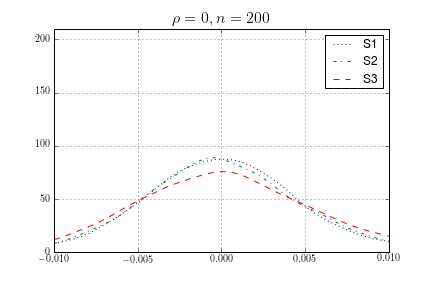
\includegraphics[width=8cm]{theta_density_200_0} & 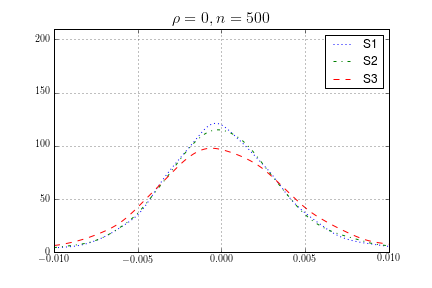
\includegraphics[width=8cm]{theta_density_500_0} \\
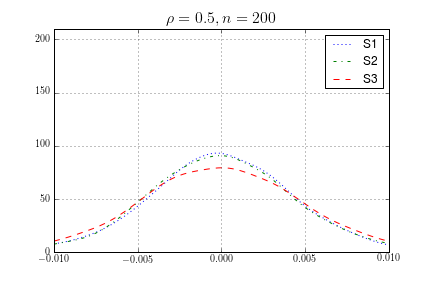
\includegraphics[width=8cm]{theta_density_200_05} & 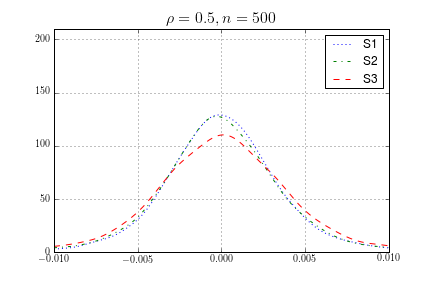
\includegraphics[width=8cm]{theta_density_500_05} \\
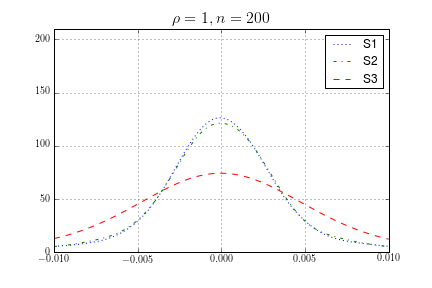
\includegraphics[width=8cm]{theta_density_200_1} & 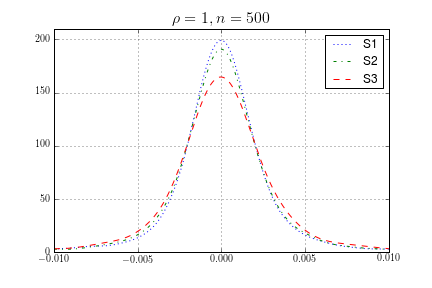
\includegraphics[width=8cm]{theta_density_500_1} \\
\end{tabular}
}
\end{table}



\clearpage

\begin{table}[!ht]
\selectfont \caption{Density estimate of $\hat{\al}_n$ (unscaled).}
\label{alpha_unscaled} \center{
\begin{tabular}{c c}
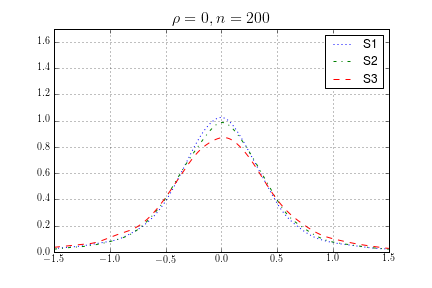
\includegraphics[width=8cm]{alpha_density_200_0} & 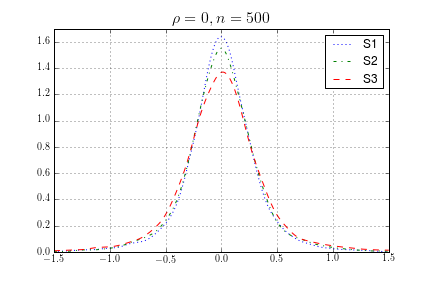
\includegraphics[width=8cm]{alpha_density_500_0} \\
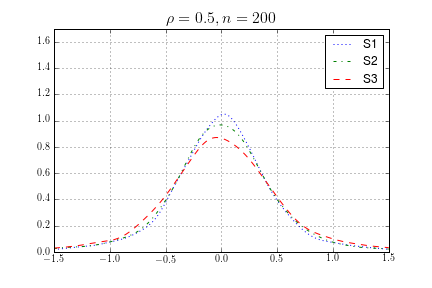
\includegraphics[width=8cm]{alpha_density_200_05} & 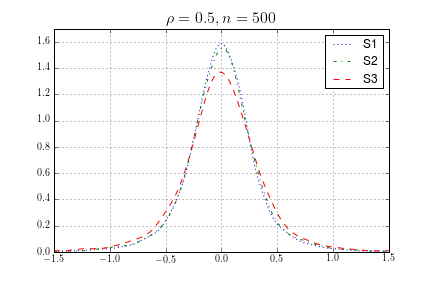
\includegraphics[width=8cm]{alpha_density_500_05} \\
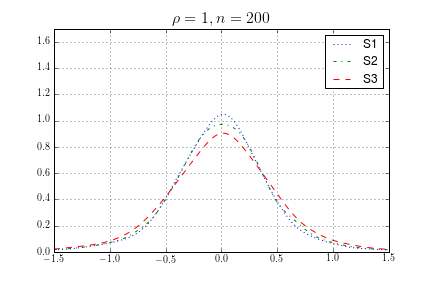
\includegraphics[width=8cm]{alpha_density_200_1} & 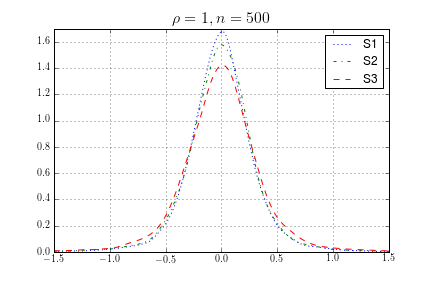
\includegraphics[width=8cm]{alpha_density_500_1} \\
\end{tabular}
}
\end{table}

\begin{table}[!ht]
\selectfont \caption{Density estimate of $\hat{\beta}_{1n}$ (unscaled).}
\label{beta1_unscaled} \center{
\begin{tabular}{c c}
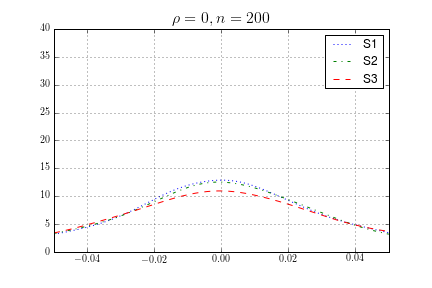
\includegraphics[width=8cm]{beta1_density_200_0} & 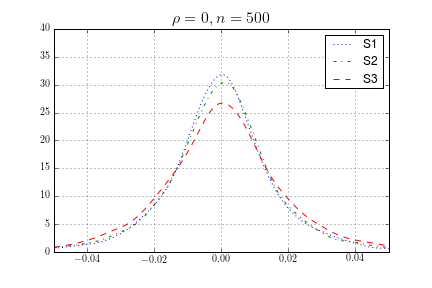
\includegraphics[width=8cm]{beta1_density_500_0} \\
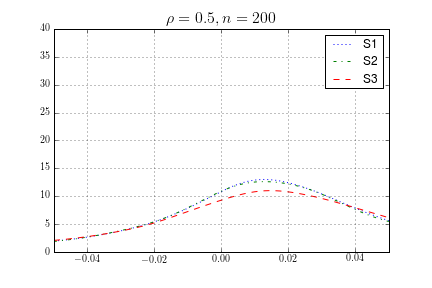
\includegraphics[width=8cm]{beta1_density_200_05} & 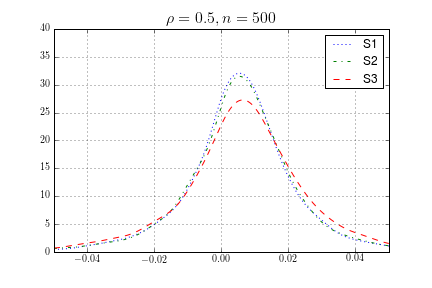
\includegraphics[width=8cm]{beta1_density_500_05} \\
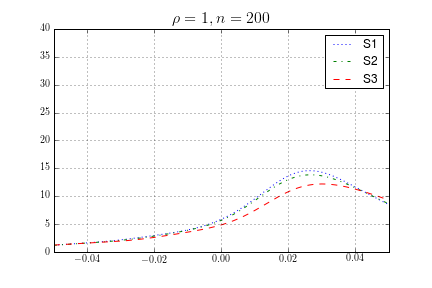
\includegraphics[width=8cm]{beta1_density_200_1} & 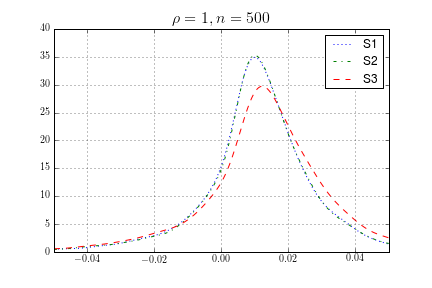
\includegraphics[width=8cm]{beta1_density_500_1} \\
\end{tabular}
}
\end{table}

\begin{table}[!ht]
\selectfont \caption{Density estimate of $\hat{\beta}_{2n}$ (unscaled).}
\label{beta2_unscaled} \center{
\begin{tabular}{c c}
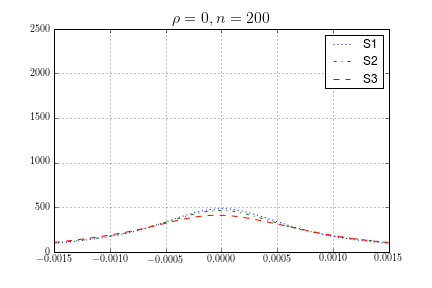
\includegraphics[width=8cm]{beta2_density_200_0} & 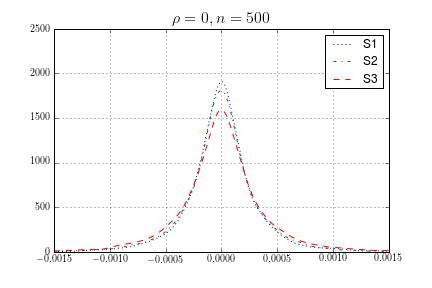
\includegraphics[width=8cm]{beta2_density_500_0} \\
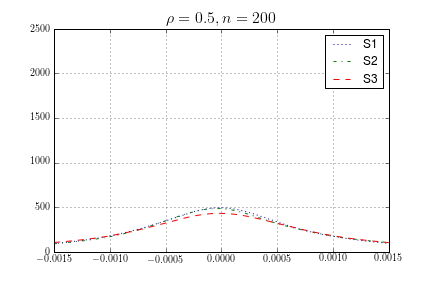
\includegraphics[width=8cm]{beta2_density_200_05} & 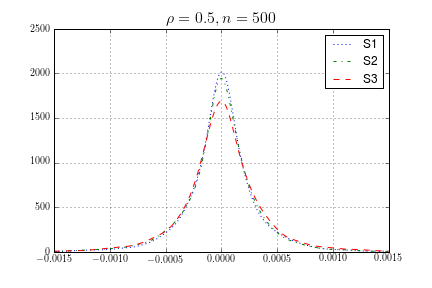
\includegraphics[width=8cm]{beta2_density_500_05} \\
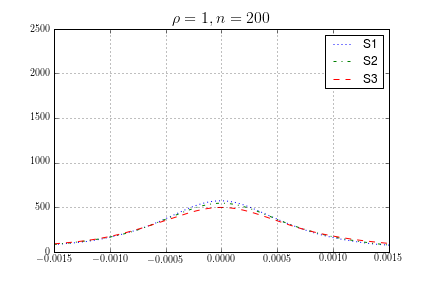
\includegraphics[width=8cm]{beta2_density_200_1} & 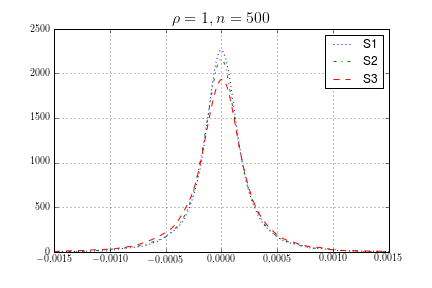
\includegraphics[width=8cm]{beta2_density_500_1} \\
\end{tabular}
}
\end{table}




\begin{table}[!ht]
\selectfont \caption{Density estimate of $\hat{\theta}_n$ (scaled by $n^{1/4}$).}
\label{theta_scaled} \center{
\begin{tabular}{c c}
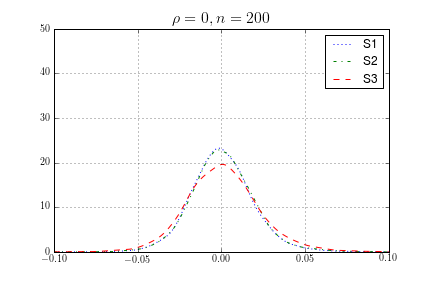
\includegraphics[width=8cm]{theta_scaled_density_200_0} & 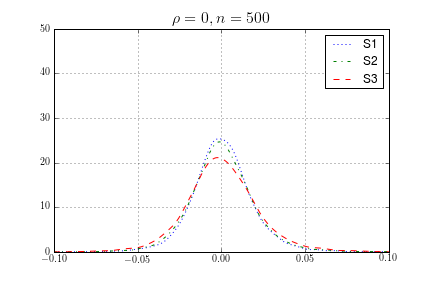
\includegraphics[width=8cm]{theta_scaled_density_500_0} \\
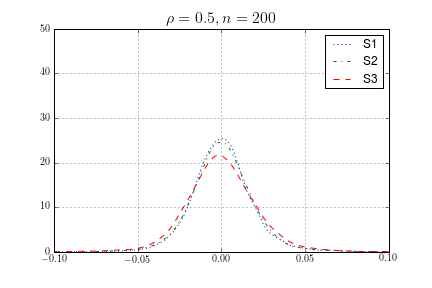
\includegraphics[width=8cm]{theta_scaled_density_200_05} & 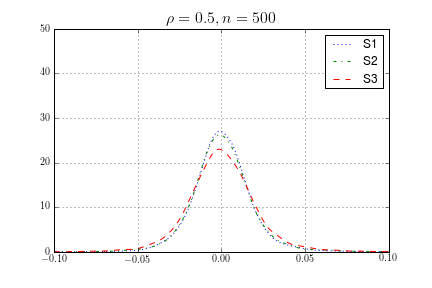
\includegraphics[width=8cm]{theta_scaled_density_500_05} \\
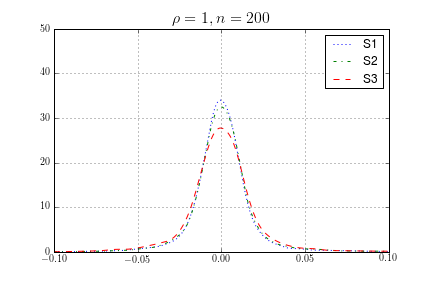
\includegraphics[width=8cm]{theta_scaled_density_200_1} & 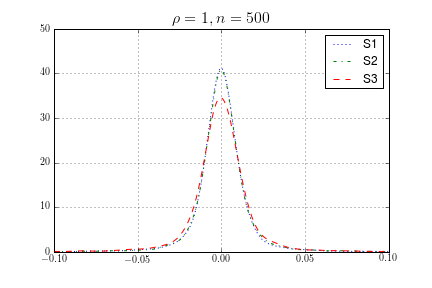
\includegraphics[width=8cm]{theta_scaled_density_500_1} \\
\end{tabular}
}
\end{table}




\begin{table}[!ht]
\selectfont \caption{Density estimate of $\hat{\alpha}_n$ (scaled by $n^{1/2}$).}
\label{alpha_scaled} \center{
\begin{tabular}{c c}
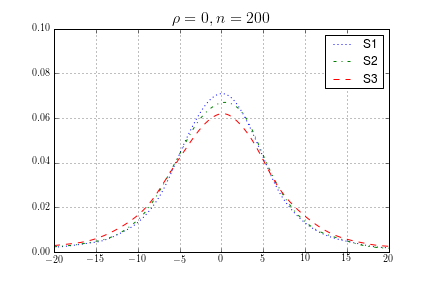
\includegraphics[width=8cm]{alpha_scaled_density_200_0} & 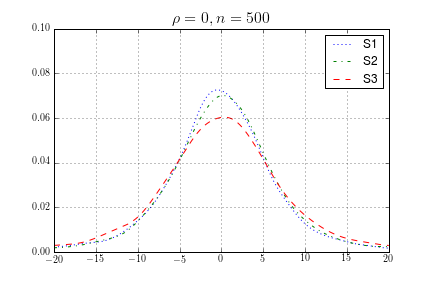
\includegraphics[width=8cm]{alpha_scaled_density_500_0} \\
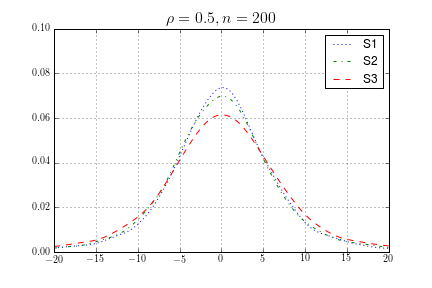
\includegraphics[width=8cm]{alpha_scaled_density_200_05} & 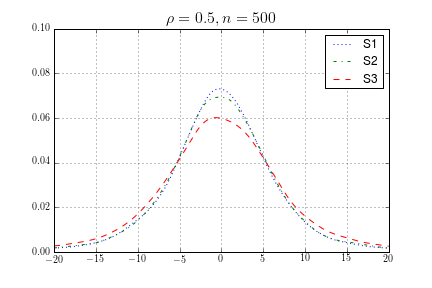
\includegraphics[width=8cm]{alpha_scaled_density_500_05} \\
\includegraphics[width=8cm]{alpha_scaled_density_200_1} & \includegraphics[width=8cm]{alpha_scaled_density_500_1} \\
\end{tabular}
}
\end{table}



\begin{table}[!ht]
\selectfont \caption{Density estimate of $\hat{\beta}_{1n}$ (scaled by $n$).}
\label{beta1_scaled} \center{
\begin{tabular}{c c}
\includegraphics[width=8cm]{beta1_scaled_density_200_0} & \includegraphics[width=8cm]{beta1_scaled_density_500_0} \\
\includegraphics[width=8cm]{beta1_scaled_density_200_05} & \includegraphics[width=8cm]{beta1_scaled_density_500_05} \\
\includegraphics[width=8cm]{beta1_scaled_density_200_1} & \includegraphics[width=8cm]{beta1_scaled_density_500_1} \\
\end{tabular}
}
\end{table}

\begin{table}[!ht]
\selectfont \caption{Density estimate of $\hat{\beta}_{2n}$ (scaled by $n^{3/2}$).}
\label{beta2_scaled} \center{
\begin{tabular}{c c}
\includegraphics[width=8cm]{beta2_scaled_density_200_0} & \includegraphics[width=8cm]{beta2_scaled_density_500_0} \\
\includegraphics[width=8cm]{beta2_scaled_density_200_05} & \includegraphics[width=8cm]{beta2_scaled_density_500_05} \\
\includegraphics[width=8cm]{beta2_scaled_density_200_1} & \includegraphics[width=8cm]{beta2_scaled_density_500_1} \\
\end{tabular}
}
\end{table}


\begin{table}[!ht]
\selectfont \caption{Density of $\hat{\theta}_n$ $t$-ratios.}
\label{theta_t} \center{
\begin{tabular}{c c}
\includegraphics[width=8cm]{theta_t_ratio_200_0} & \includegraphics[width=8cm]{theta_t_ratio_500_0} \\
\includegraphics[width=8cm]{theta_t_ratio_200_05} & \includegraphics[width=8cm]{theta_t_ratio_500_05} \\
\includegraphics[width=8cm]{theta_t_ratio_200_1} & \includegraphics[width=8cm]{theta_t_ratio_500_1} \\
\end{tabular}
}
\end{table}



\begin{table}[!ht]
\selectfont \caption{Density of $\hat{\alpha}_n$ $t$-ratios.}
\label{alpha_t} \center{
\begin{tabular}{c c}
\includegraphics[width=8cm]{alpha_t_ratio_200_0} & \includegraphics[width=8cm]{alpha_t_ratio_500_0} \\
\includegraphics[width=8cm]{alpha_t_ratio_200_05} & \includegraphics[width=8cm]{alpha_t_ratio_500_05} \\
\includegraphics[width=8cm]{alpha_t_ratio_200_1} & \includegraphics[width=8cm]{alpha_t_ratio_500_1} \\
\end{tabular}
}
\end{table}



\begin{table}[!ht]
\selectfont \caption{Density of $\hat{\beta}_{1n}$ $t$-ratios.}
\label{beta1_t} \center{
\begin{tabular}{c c}
\includegraphics[width=8cm]{beta1_t_ratio_200_0} & \includegraphics[width=8cm]{beta1_t_ratio_500_0} \\
\includegraphics[width=8cm]{beta1_t_ratio_200_05} & \includegraphics[width=8cm]{beta1_t_ratio_500_05} \\
\includegraphics[width=8cm]{beta1_t_ratio_200_1} & \includegraphics[width=8cm]{beta1_t_ratio_500_1} \\
\end{tabular}
}
\end{table}



\begin{table}[!ht]
\selectfont \caption{Density of $\hat{\beta}_{2n}$ $t$-ratios.}
\label{beta2_t} \center{
\begin{tabular}{c c}
\includegraphics[width=8cm]{beta2_t_ratio_200_0} & \includegraphics[width=8cm]{beta2_t_ratio_500_0} \\
\includegraphics[width=8cm]{beta2_t_ratio_200_05} & \includegraphics[width=8cm]{beta2_t_ratio_500_05} \\
\includegraphics[width=8cm]{beta2_t_ratio_200_1} & \includegraphics[width=8cm]{beta2_t_ratio_500_1} \\
\end{tabular}
}
\end{table}

\begin{table}[!ht]
\selectfont \caption{Estimate and 95\% Confidence Interval of $\hat{\al}_n$}
\label{alpha_plot} \center{
\begin{tabular}{c}
\includegraphics[width=16cm]{a_plot}
\end{tabular}
}
\end{table}

% \begin{table}[!ht]
% \selectfont \caption{Estmate and 95\% Confidence Interval of $\hat{\theta}_n = (\hat{\al}_n, \hat{\beta}_{1n}, \hat{\beta}_{2n})$}
% \label{GseqTable} \center{
% \begin{tabular}{c}
% %\includegraphics[width=16cm]{a_plot} \\
% \includegraphics[width=16cm]{b_1_plot} \\
% \includegraphics[width=16cm]{b_2_plot} \\
% \end{tabular}
% }
% \end{table}


\begin{table}[!ht]
\selectfont \caption{Confidence Intervals (95\% confidence) of $\hat{\alpha}_{n}$.}
\label{alpha_est} \center{
\begin{tabular}{|c |c  c  c|}
\hline
Country & $\hat{\alpha}_{n}$ & Lower & Upper \\
\hline
AUS & -57.387 & -58.005 & -56.769 \\
AUT & -25.352 & -26.414 & -24.290 \\
BEL & -41.632 & -43.144 & -40.121 \\
CAN & -44.442 & -45.615 & -43.268 \\
CHN & -32.402 & -38.126 & -26.678 \\
DEN & -113.670 & -115.375 & -111.965 \\
FIN & -91.869 & -94.019 & -89.720 \\
FRA & -76.449 & -78.162 & -74.735 \\
HOL & -71.892 & -73.439 & -70.344 \\
IND & -59.854 & -60.930 & -58.779 \\
IRE & -33.058 & -34.265 & -31.851 \\
ITA & -71.375 & -72.604 & -70.146 \\
JAP & -27.674 & -29.293 & -26.056 \\
NOR & -58.519 & -60.442 & -56.597 \\
USA & -45.950 & -46.945 & -44.954 \\
\hline
\end{tabular}
}
\end{table}



\begin{table}[!ht]
\selectfont \caption{Confidence Intervals (95\% confidence) of $\hat{\beta}_{1n}$.}
\label{beta1_est} \center{
\begin{tabular}{|c |c  c  c|}
\hline
Country & $\hat{\beta}_{1n}$ & Lower & Upper \\
\hline
AUS & 11.520 & 10.810 & 12.230 \\
AUT & 5.075 & 4.193 & 5.958 \\
BEL & 9.116 & 7.922 & 10.310 \\
CAN & 9.217 & 8.114 & 10.321 \\
CHN & 7.609 & 5.063 & 10.154 \\
DEN & 23.724 & 22.242 & 25.205 \\
FIN & 18.967 & 17.225 & 20.709 \\
FRA & 16.443 & 15.000 & 17.886 \\
HOL & 14.921 & 13.579 & 16.262 \\
IND & 14.908 & 13.894 & 15.923 \\
IRE & 6.816 & 6.062 & 7.570 \\
ITA & 14.502 & 13.647 & 15.356 \\
JAP & 5.447 & 4.614 & 6.279 \\
NOR & 11.802 & 10.555 & 13.050 \\
USA & 9.536 & 8.449 & 10.623 \\
\hline
\end{tabular}
}
\end{table}


\begin{table}[!ht]
\selectfont \caption{Confidence Intervals (95\% confidence) of $\hat{\beta}_{2n}$.}
\label{beta2_est} \center{
\begin{tabular}{|c |c  c  c|}
\hline
Country & $\hat{\beta}_{2n}$ & Lower & Upper \\
\hline
AUS & -0.562 & -0.730 & -0.394 \\
AUT & -0.246 & -0.389 & -0.102 \\
BEL & -0.485 & -0.721 & -0.248 \\
CAN & -0.462 & -0.732 & -0.192 \\
CHN & -0.446 & -0.775 & -0.118 \\
DEN & -1.226 & -1.586 & -0.865 \\
FIN & -0.967 & -1.256 & -0.678 \\
FRA & -0.875 & -1.190 & -0.559 \\
HOL & -0.762 & -1.093 & -0.432 \\
IND & -0.945 & -1.174 & -0.715 \\
IRE & -0.341 & -0.443 & -0.238 \\
ITA & -0.729 & -0.882 & -0.576 \\
JAP & -0.258 & -0.365 & -0.151 \\
NOR & -0.586 & -0.822 & -0.351 \\
USA & -0.477 & -0.768 & -0.186 \\
\hline
\end{tabular}
}
\end{table}



%%% Local Variables: 
%%% mode: latex
%%% TeX-master: "../thesis"
%%% End: 


%\backmatter % book mode only
%\appendix
\begin{appendices}
\chapter{Appdx A}

and here I put a bit of postamble ...

% ------------------------------------------------------------------------

%%% Local Variables: 
%%% mode: latex
%%% TeX-master: "../thesis"
%%% End: 

\chapter{Appdx B}

and here I put some more postamble ...

% ------------------------------------------------------------------------

%%% Local Variables: 
%%% mode: latex
%%% TeX-master: "../thesis"
%%% End: 

\chapter{Limit theorems for functional of normalised sum} \la{chap:app3}

This appendix gives the following theorem, which comes from \cite{wangphillips2010a}. We list the following assumptions.

\begin{assump} \la{assump:A:integrable}
$|g(x)|$ and $g^2(x)$ are Lebesgue integrable functions on $R$ with $\tau \equiv \int g(x) dx \ne 0$.
\end{assump}

\begin{assump} \la{assump:A:weakConvergence}
There exists a stochastic process $G(t)$ having a continuous local time $L_{G}(t,s)$ such that $x_{[nt],n}\Rightarrow G(t)$, on $D[0,1]$, where weak convergence is understood w.r.t the Skorohod topology on the space $D[0,1]$.
\end{assump}

\newenvironment{assump_1}{ \par \medskip\noindent  {\bf Assumption \ref{assump:A:weakConvergence}*.}}{\par\medskip}

\begin{assump_1} 
On a suitable probability space, there exists a stochastic process $G(t)$ having a continuous local time $L_G(t, s)$ such that $\sup_{0 \le t \le 1} | x_{[nt], n} - G(t) | = o_P(1)$.
\end{assump_1}

\begin{assump} \la{assump:A:density}
 For all $0\leq k<l\leq n,n\geq 1$, there exist a sequence of constants $d_{l,k,n}\sim C_0 [n/(l-k)]^{-d}$ for some $0< d<1$ and a sequence of increasing $\sigma $-fields ${\mathcal F}_{k,n}$ (define ${\mathcal F}_{0,n}=\sigma \{\phi ,\Omega \}$\textit{, the trivial }$\sigma $-field such that $x_{k,n}$ are adapted to ${\mathcal F}_{k,n}$ and, conditional on ${\mathcal F}_{k,n}$, $(x_{l,n}-x_{k,n})/d_{l,k,n}$ has a density $h_{l,k,n}(x)$ satisfying that $h_{l,k,n}(x)$ is uniformly bounded by a constant $K$ and uniformly for $j-k$ sufficiently large
 \be
 \sup_y | h_{l,k,n}(y + u) - h_{l,k,n}(y)| \le C \min\{|u|, 1\}. \la {eqn:app3:77}
\ee
\end{assump}

As Assumptions \ref{assump:A:density} implies Assumption 2.3 in \cite{wangphillips2010a}, the following theorem comes from Theorem 2.2 of \cite{wangphillips2010a}.

\begin{thm}
Suppose Assumptions \ref{assump:A:integrable}--\ref{assump:A:density} hold. Then, for any $c_n \to \infty$, $c_n / n \to 0$, and $r \in [0, 1]$,
\be
\frac{c_n}{n}\sum_{k = 1}^{[nr]} g(c_n x_{k,n}) \to_D \tau L_G(r, 0).
\ee
If Assumption \ref{assump:A:weakConvergence} is replaced by Assumption \ref{assump:A:weakConvergence}*, then, for any $c_n \to \infty$ and $c_n / n \to 0$,
\be
\sup_{0 \le r \le 1} \Big | \frac{c_n}{n} \sum_{k = 1}^{[nr]} g(c_n x_{k,n}) - \tau L_G(r, 0) \Big | \to_P 0,
\ee
under the same probability space defined as in Assumption \ref{assump:A:weakConvergence}*.
\end{thm}


% ------------------------------------------------------------------------

%%% Local Variables: 
%%% mode: latex
%%% TeX-master: "../thesis"
%%% End: 

\chapter{List of Publications}

{\bf Part I.} Related to this thesis
\begin{enumerate}
\item ``Uniform convergence rates for a class of martingales with application in non-linear co-integrating regression" (with Qiying Wang). Accepted by {\it Bernoulli}, (Chapter 2 and part of Chapter 5 are from this paper).
\item ``Uniform convergence for nonparametric estimators with non-stationary data" (with Qiying Wang). Accepted by {\it Econometric Theory}, (Chapter 3 and part of Chapter 5 are from this paper).
\item ``Nonlinear regressions with nonstationary time series" (with Qiying Wang). Revised and resubmitted to {\it Journal of Econometrics}, (Chapter 7 is from this paper).
\item ``Testing for a unit root with non-stationary volatility" (with Qiying Wang). {\it Manuscript in preparation}, (Chapter 6 is from this paper).
\item ``Uniform approximation to local time with applications in non-linear co-integrating regression" (with Wei Dong Liu and Qiying Wang). {\it Manuscript in preparation}, (Chapter 4 is from this paper).
\end{enumerate}

\medskip
\noindent
{\bf Part II.} Publications of author in other projects
\begin{enumerate}
\item ``Doubly resolvable nearly Kirkman triple systems" (with Julian Abel, Charles Colbourn, Esther Lamken, Chengmin Wang and Jinhua Wang). {\it Journal of Combinatorial Designs}, doi: 10.1002/jcd.21342.
\item ``Existence of GBRDs with block size 4 and BRDs with block size 5" (with Julian Abel, Diana Combe and William Palmer), {\it Designs, Codes and Cryptography}, {\bf 61(3)}, 285--300.
\item ``Existence of doubly near resolvable $(v, 4, 3)$ BIBDs" (with Julian Abel), {\it Australasian Journal of Combinatorics}, {\bf 47}, 109--124.
\end{enumerate}

% ------------------------------------------------------------------------

%%% Local Variables: 
%%% mode: latex
%%% TeX-master: "../thesis"
%%% End: 

\end{appendices}

\bibliographystyle{apalike}
%\bibliographystyle{plainnat}
%\bibliographystyle{Classes/CUEDbiblio}
%\bibliographystyle{Classes/jmb}
%\bibliographystyle{Classes/jmb} % bibliography style
\renewcommand{\bibname}{References} % changes default name Bibliography to References
\bibliography{References/references} % References file

\end{document}
